\documentclass[b5paper, 12pt]{book}

% Enable numbering for subsubsections
\setcounter{secnumdepth}{3}

\usepackage{graphicx} % Required for inserting images
\usepackage{soul} % For highlightin
\usepackage{xcolor}
\usepackage{url}
\usepackage{geometry} % For custom page layout
\usepackage{amsmath}
\usepackage[hidelinks]{hyperref}
\usepackage{breakurl}
\usepackage{amssymb}
\usepackage{fancyhdr} % For customizing headers
\usepackage{breqn}
\usepackage{rotating}
\usepackage{float}
% \usepackage{titling}
\usepackage{titlesec}
\usepackage{booktabs}
\usepackage{caption}
\usepackage{subfiles}
% \usepackage{capt-of}  % For the caption handling

\usepackage[utf8]{inputenc}
\usepackage[T1]{fontenc}
\usepackage{ebgaramond}
\usepackage{listings}
\usepackage{ragged2e}
\usepackage{amsthm}
\usepackage{colortbl}
% \usepackage{etoolbox}
\usepackage{hyphenat}
% \usepackage[toc, acronym, section=chapter]{glossaries}
\usepackage[toc, acronym, nonumberlist, section=chapter]{glossaries}
% \usepackage{xr}

\hyphenation{res-i-dues}
\hyphenation{Alpha-Fold}
\hyphenation{Shift-Crypt}

% Reduce chapter title size but keep "Chapter" above the title
\titleformat{\chapter}[display]
  {\normalfont\Large\bfseries}{\chaptername\ \thechapter}{10pt}{\Large}

  % Adjust spacing before and after chapter title
\titlespacing*{\chapter}{0pt}{-10pt}{10pt} % {left}{before-sep}{after-sep}

% Define a simple abstract environment
\newcommand{\abstractname}{Abstract} % Define abstract name
\newenvironment{abstract}{%
    \setlength{\emergencystretch}{10em}% Adjust as necessary
    \noindent\textbf{\abstractname}\par\medskip
    \ignorespaces
}{%
    \par
    \setlength{\emergencystretch}{0em} % Reset to default value
    \ignorespacesafterend
}

\usepackage{xcolor} % For defining colors and highlighting
% Highlight added by JG to highlight revision changes
% \renewcommand{\textcolor}[2]{ #2 }

% Define custom colors for syntax highlighting
\definecolor{codegreen}{rgb}{0,0.6,0}
\definecolor{codegray}{rgb}{0.5,0.5,0.5}
\definecolor{codepurple}{rgb}{0.58,0,0.82}
\definecolor{backcolour}{rgb}{0.95,0.95,0.95}

% Setup the lstlisting environment
\lstset{
    language=Python,                % Specify the language
    % Removed backgroundcolor for transparency
    commentstyle=\color{codegreen},
    backgroundcolor=\color{backcolour}, 
    keywordstyle=\color{magenta},
    numberstyle=\tiny\color{codegray},
    stringstyle=\color{codepurple},
    basicstyle=\ttfamily\footnotesize, % Monospaced font
    breakatwhitespace=false,         
    breaklines=true,                 % Allows line breaks
    captionpos=b,                    % Caption position bottom, can be removed if no caption
    keepspaces=true,                 % Preserves spaces in text, useful for indentation
    numbers=left,                    % Line numbers on left
    numbersep=5pt,                   % How far the line-numbers are from the code
    showspaces=false,                % Do not show spaces everywhere as underscores
    showstringspaces=false,          % Do not show spaces in strings
    showtabs=false,                  % Do not show tabs within strings adding particular underscores
    tabsize=1,                       % Sets default tabsize to 2 spaces
    % frame=single,                    % Adds a frame around the code
    numbers=none,
    }



% Set the font size for all figure and table captions
\captionsetup{font=small}

% % Define the Supplementary Data environment
% \newcounter{suppdata}
% \renewcommand{\thesuppdata}{\arabic{suppdata}}
% \newenvironment{suppdata}{%
%   \refstepcounter{suppdata}%
%   \noindent\textbf{Supplementary Data~\thesuppdata}\quad%
%   \label{suppdata\thesuppdata}%
% }{\bigskip}

\newcounter{suppdata}
\renewcommand{\thesuppdata}{\thechapter.\arabic{suppdata}}
\newenvironment{suppdata}{%
  \refstepcounter{suppdata}%
  \noindent\textbf{Supplementary Data~\thesuppdata}\quad%
  \label{suppdata\thesuppdata}%
}{\bigskip}

% Change the caption name from "Listing" to "Snippet"
\renewcommand{\lstlistingname}{Code snippet}

% % Custom reference commands
\newcommand{\figref}[1]{Fig.~\ref{#1}}
\newcommand{\tableref}[1]{Table~\ref{#1}}
\newcommand{\suppfigref}[1]{Supplementary Fig.~\ref{#1}}
\newcommand{\supptableref}[1]{Supplementary Table~\ref{#1}}
\newcommand{\suppdataref}[1]{Supplementary Data~\ref{#1}}

% Load supplementary documents to cross-reference
% \externaldocument[supp:]{supplementary_figures}
% \externaldocument[supp:]{supplementary_tables}
% \externaldocument[supp:]{supplementary_data}
% \externaldocument[supp:]{supplementary_information}

% Define commands for referencing supplementary materials
% \newcommand{\suppfigref}[1]{Supplementary Fig.~\ref{supp:#1}}
% \newcommand{\supptableref}[1]{Supplementary Table~\ref{supp:#1}}
% \newcommand{\suppdataref}[1]{Supplementary Data~\ref{supp:#1}}

% Increase tolerance for line breaks
\tolerance=2000
% Allow more stretch between words
\emergencystretch=10pt


% \title{Vrije Universiteit Brussel\\ \vspace{1cm} % Add "Vrije Universiteit Brussel" at the top
% Probabilistic description of protein backbone motions and conformations}
% \author{
%     \begin{tabular}{@{}c@{}}
%     Author:\\Jose Gavaldá-García
%     \end{tabular}
%     \hspace{2cm} % Horizontal space between columns
%     \begin{tabular}{@{}c@{}}
%     Supervisor:\\Prof. Dr. Wim F. Vranken
%     \end{tabular}
% }
% \date{2024\\ \vspace{1cm}
% \large{Dissertation presented in fulfilment of the requirements for the Ph.D. degree in Bio-engineering Sciences at the Vrije Universiteit Brussel}}

% \begin{document}
% \frontmatter
% \maketitle

% % Adding the logos at the bottom of the title page
% \vspace*{\fill} % Add flexible vertical space to push logos to the bottom
% \begin{center}
%     \begin{tabular}{cccc}
%         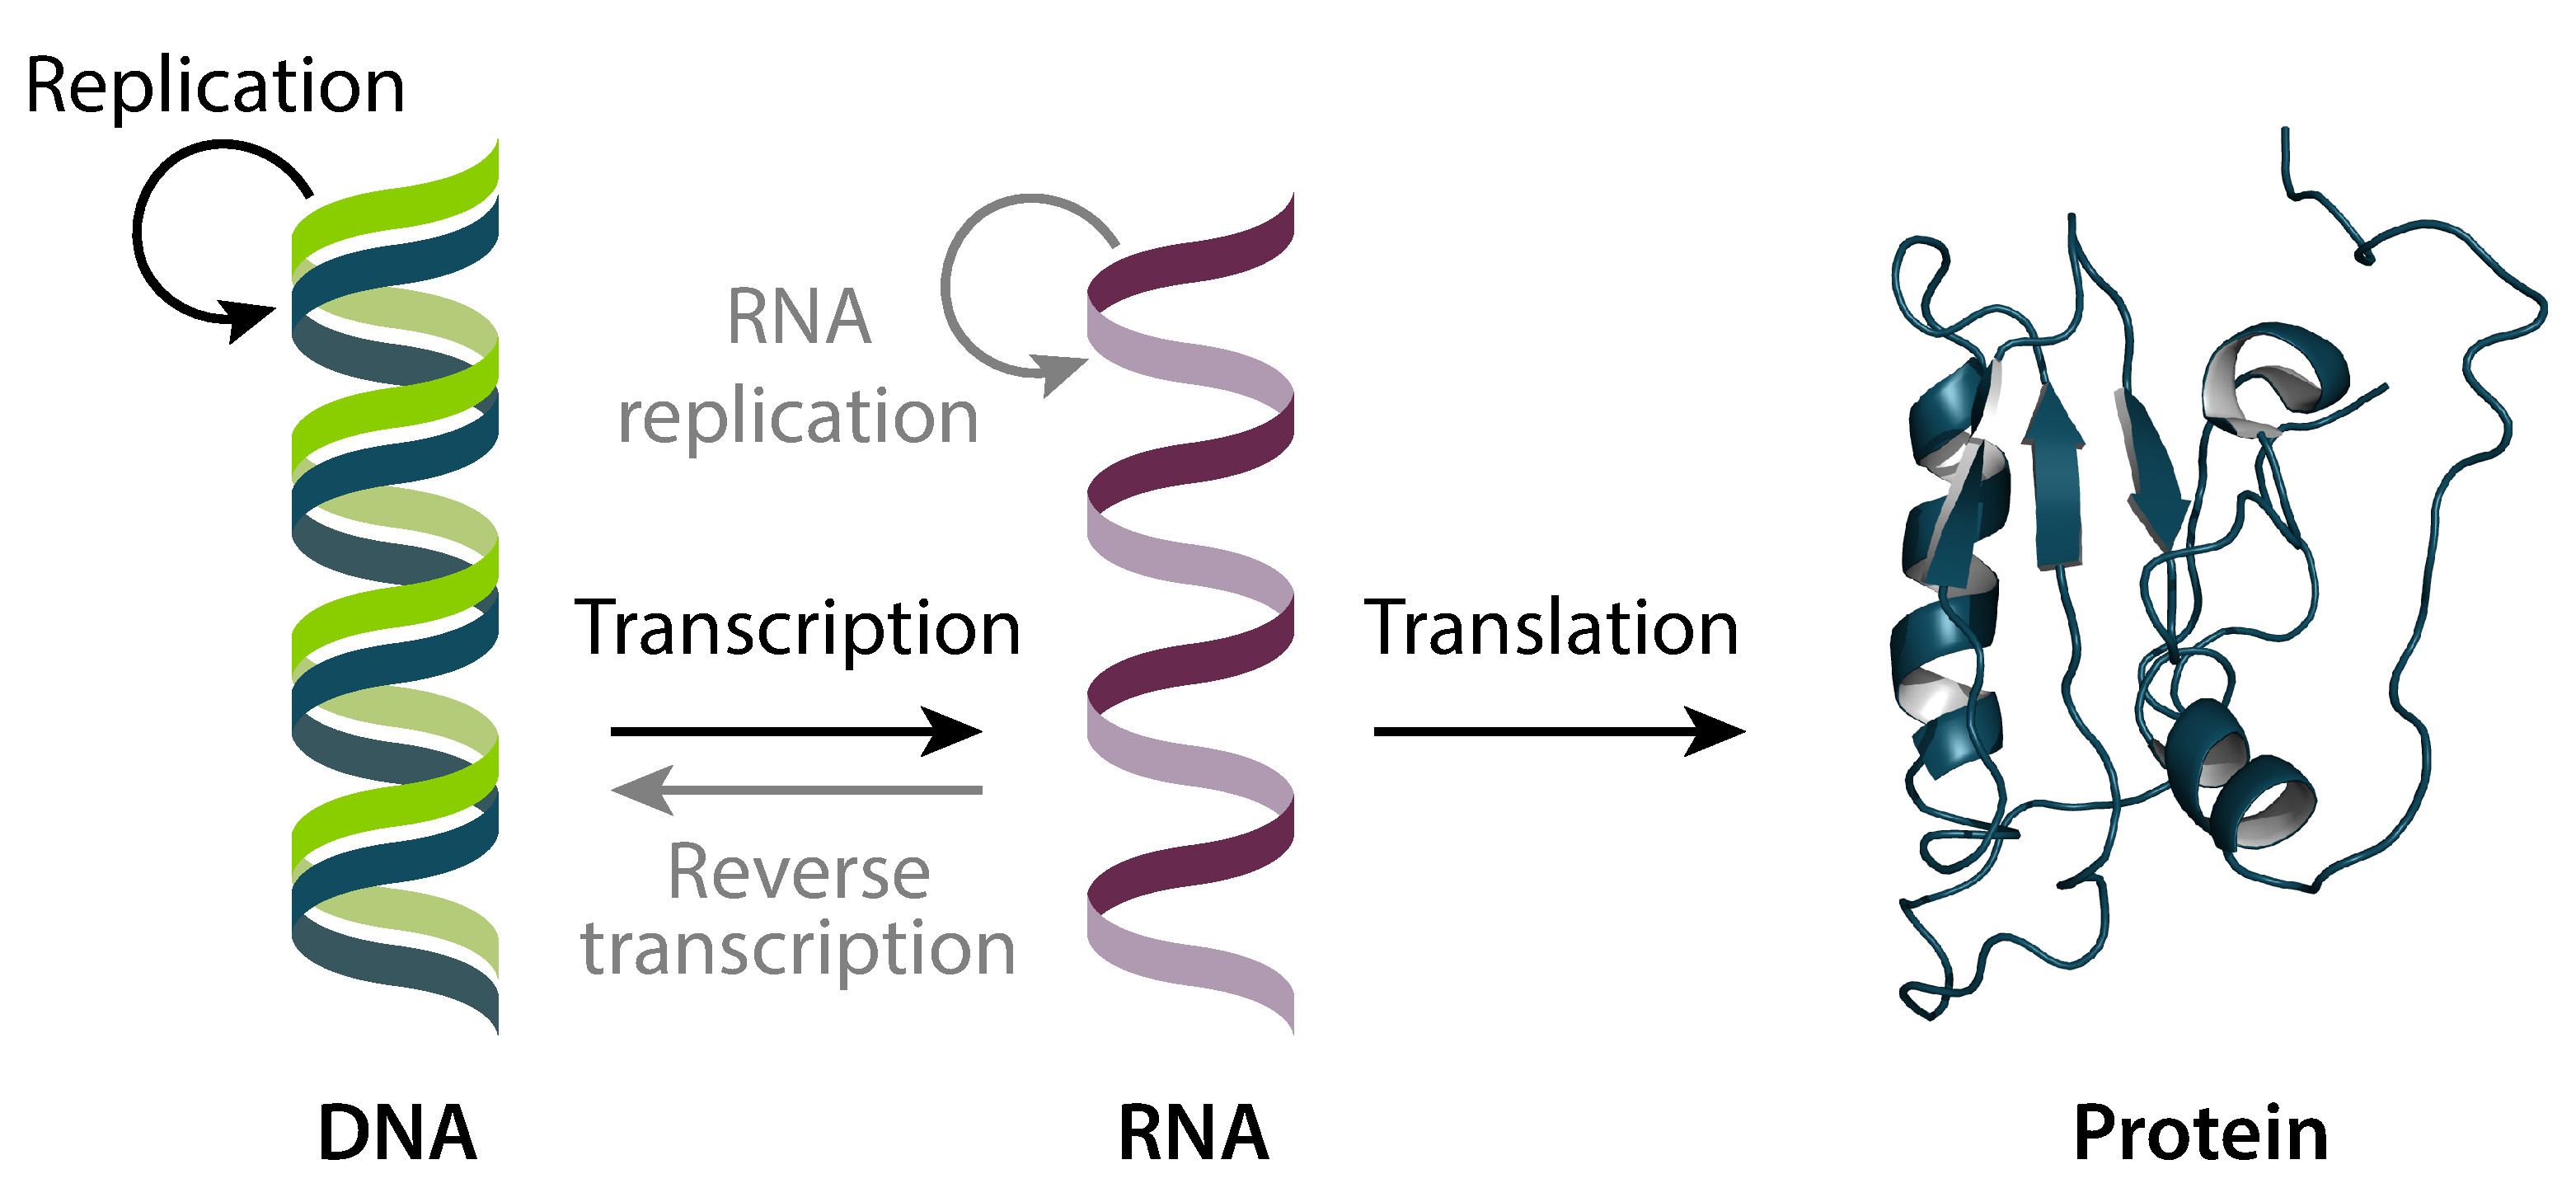
\includegraphics[width=0.2\textwidth]{figures/central_dogma.pdf} &
%         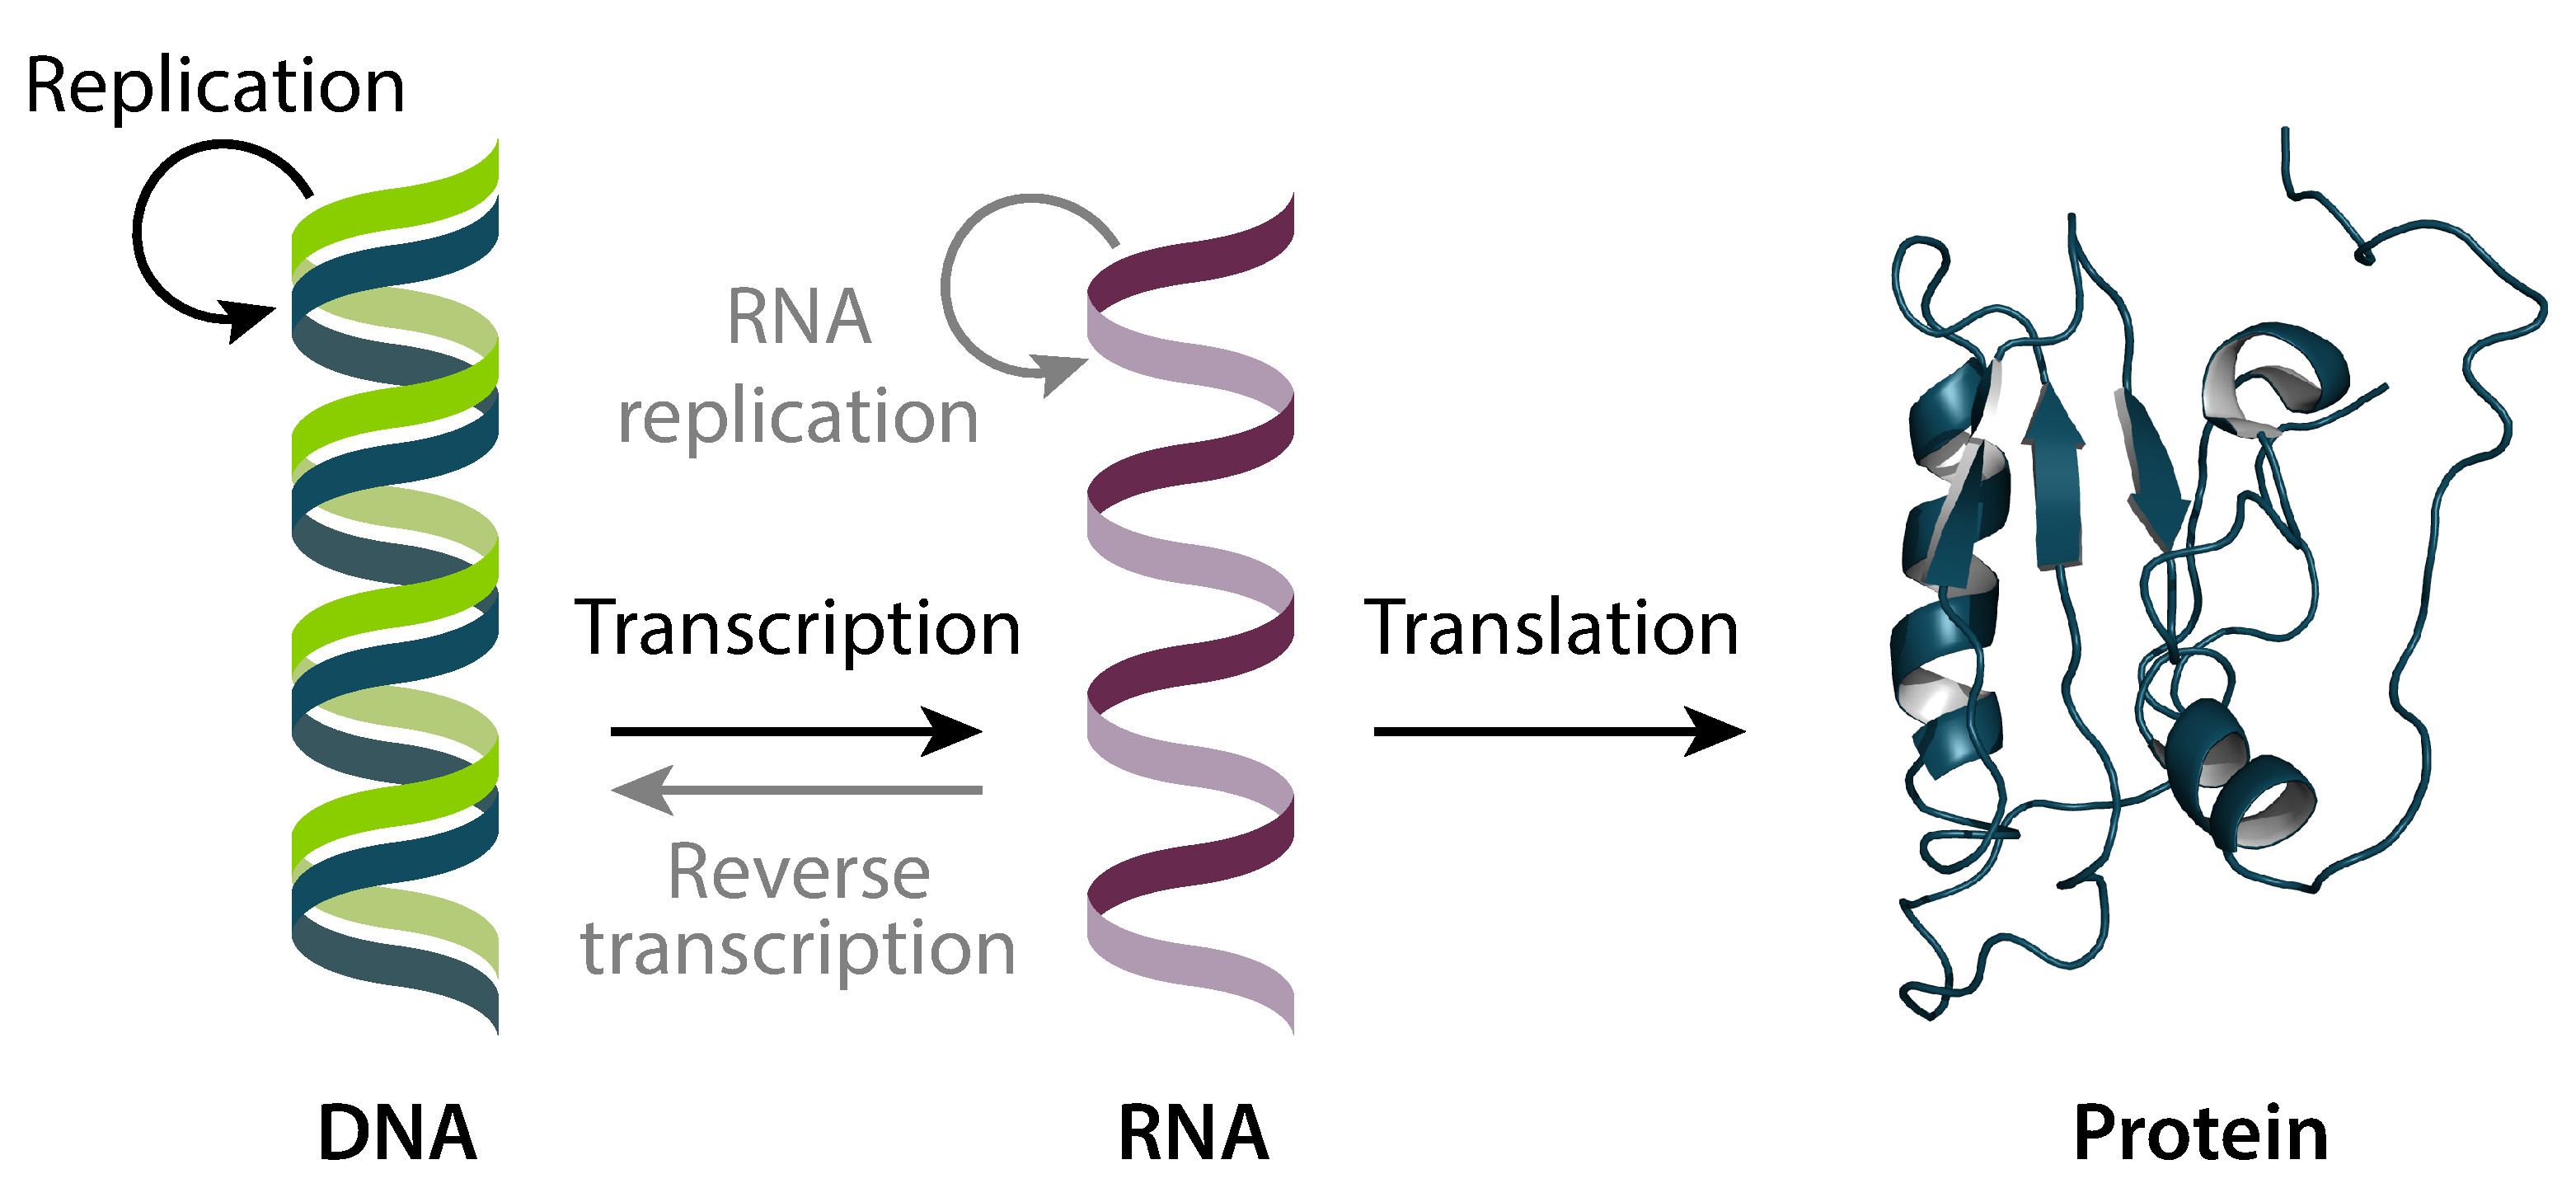
\includegraphics[width=0.2\textwidth]{figures/central_dogma.pdf} &
%         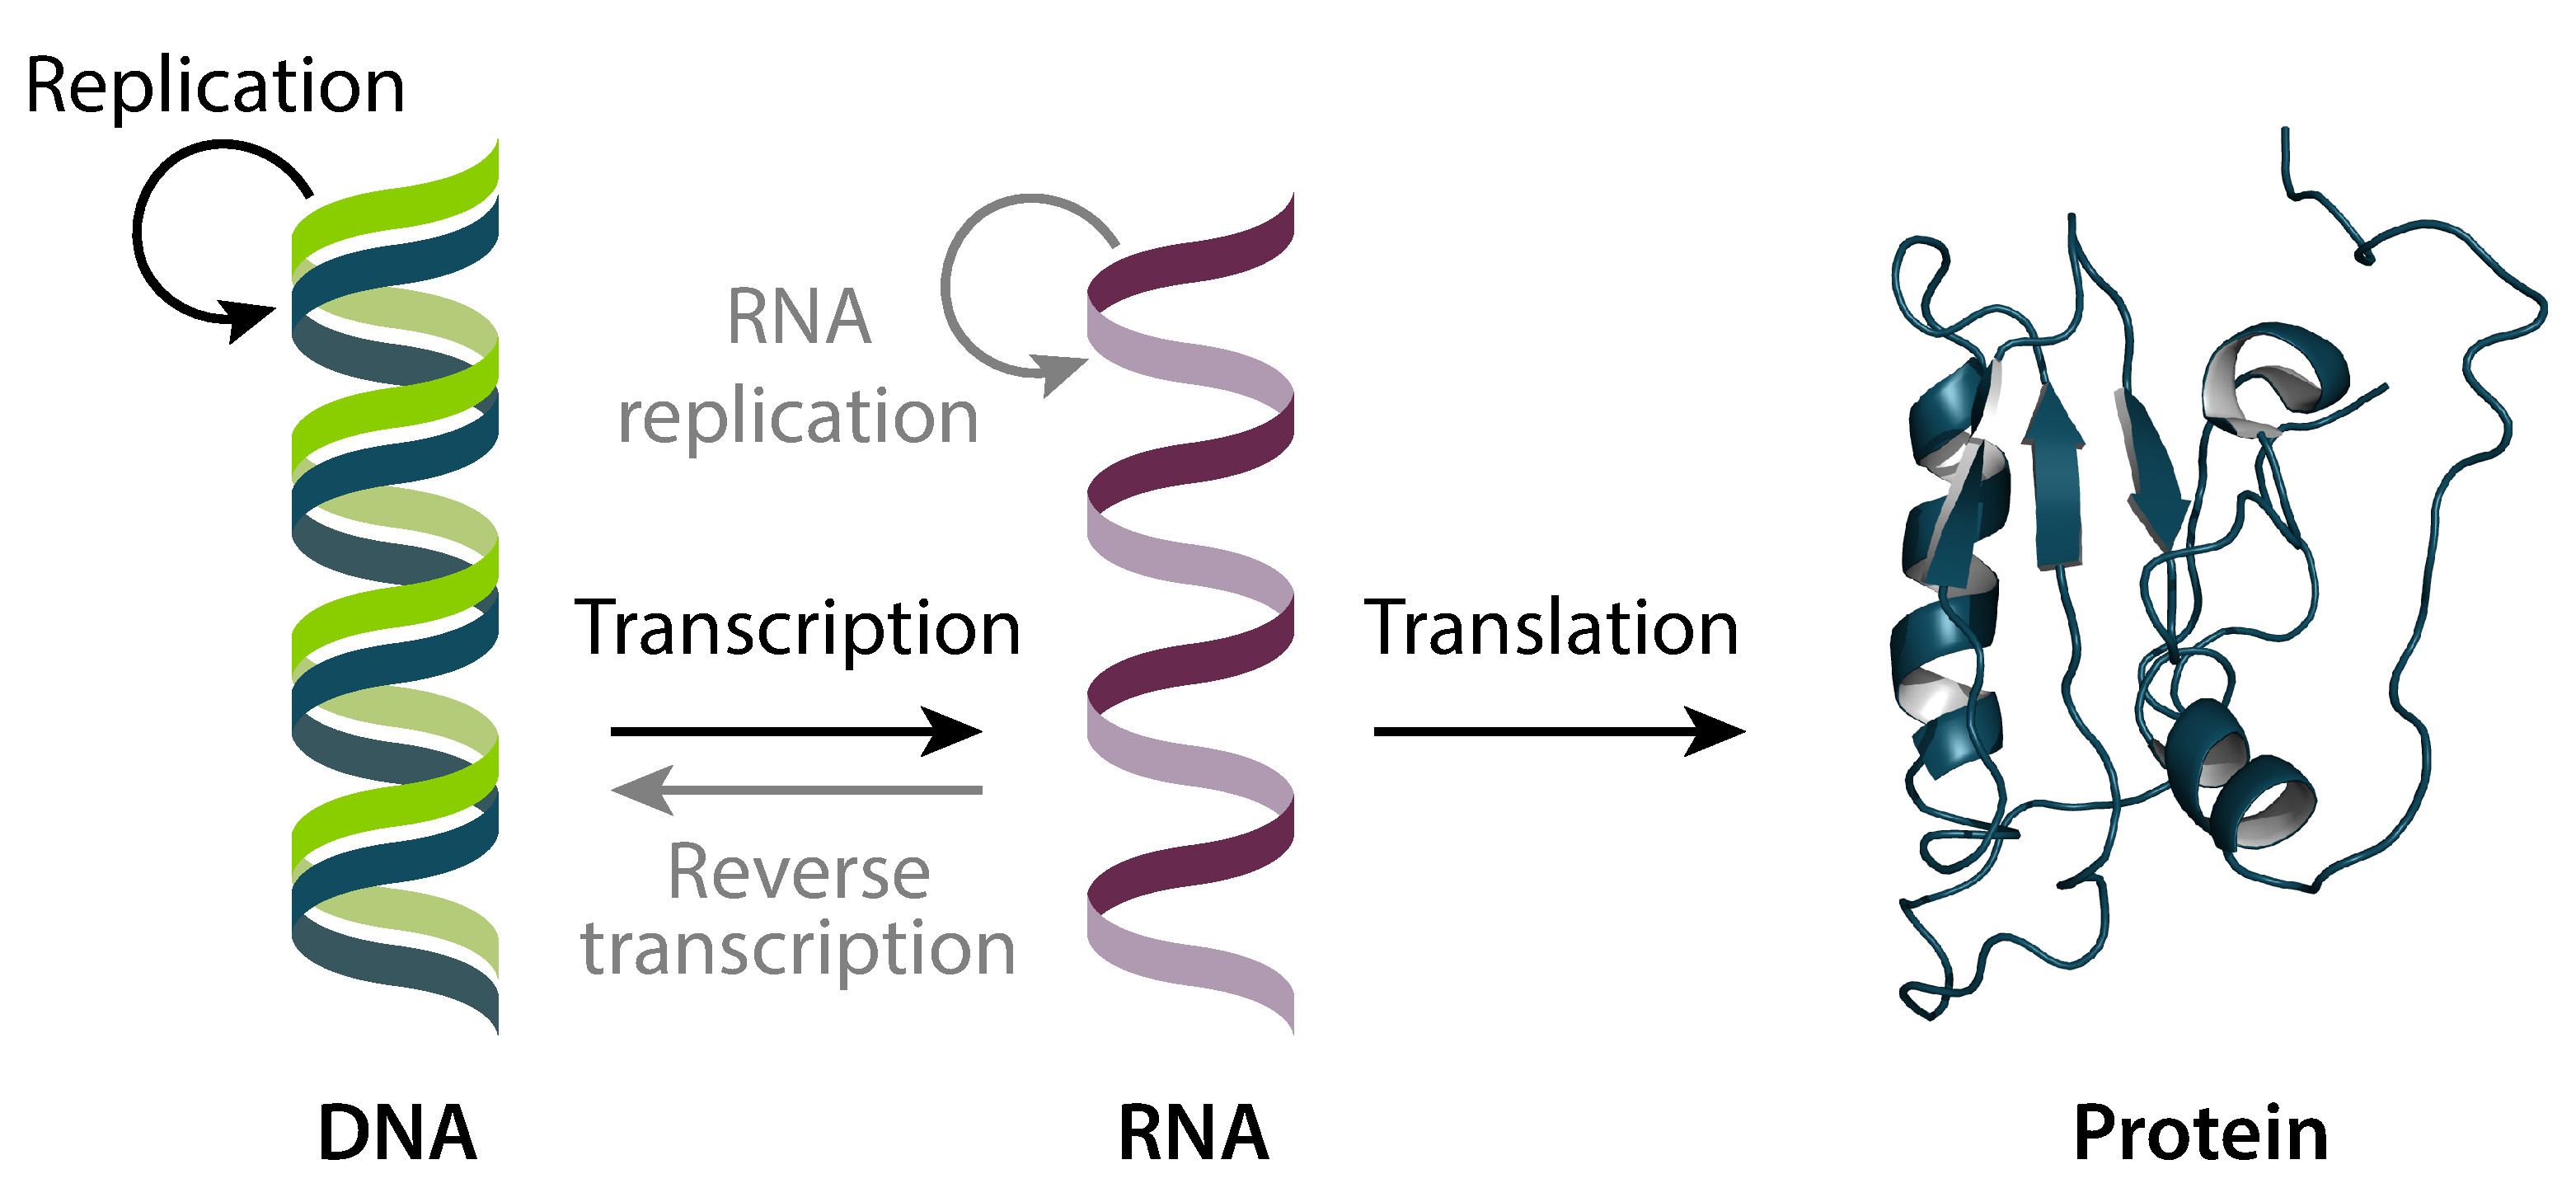
\includegraphics[width=0.2\textwidth]{figures/central_dogma.pdf} &
%         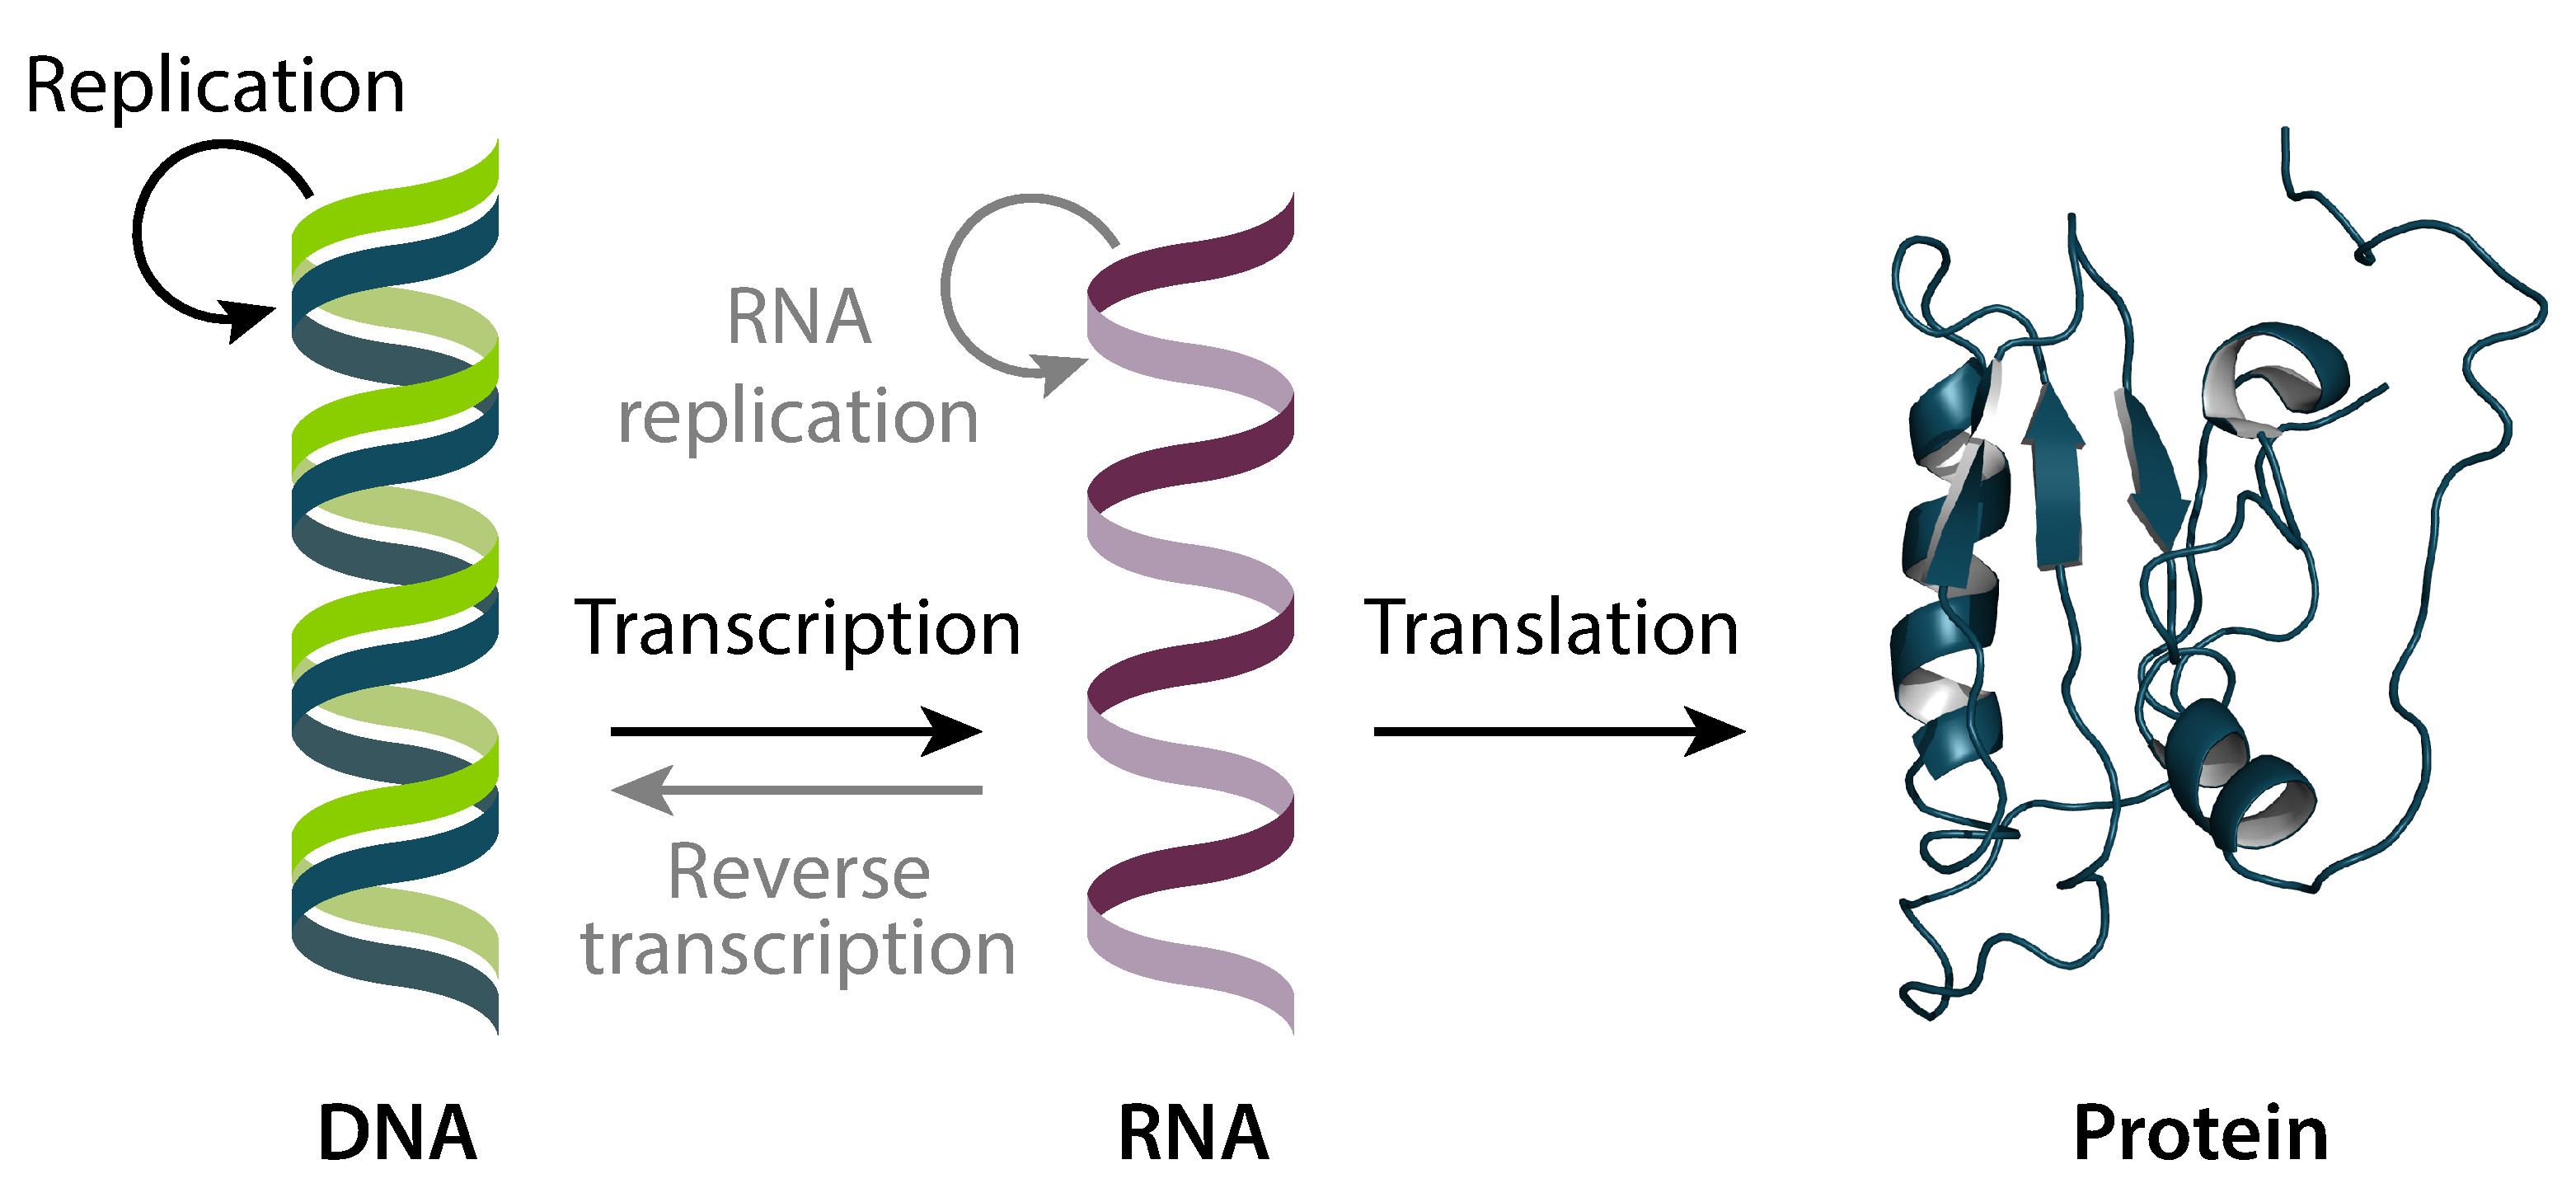
\includegraphics[width=0.2\textwidth]{figures/central_dogma.pdf} \\
%     \end{tabular}
% \end{center}
% \vspace*{\fill} % Add flexible vertical space below logos as well

\makeglossaries
% glossary_entries.tex
\newglossaryentry{flexibility}{
  name={Flexibility, Protein Flexibility},
  description={Property of a protein or protein region to adopt multiple energetically accessible conformations},
  text=flexibility
}

\newglossaryentry{dynamics}{
  name={Dynamics, Protein Dynamics},
  description={Property of a protein or protein region to transition between conformations over time},
  text=dynamics
}

\newglossaryentry{accuracy}{
  name=Accuracy,
  description={The degree to which a measurement or prediction conforms to the true value or the standard. It is defined as:\newline   \[ \text{Accuracy} = \frac{\text{True Positives} + \text{True Negatives}}{\text{Total Instances}} \]},
  text=accuracy
}

\newglossaryentry{proteinstructure}{
  name=Protein structure,
  description={Three-dimensional arrangement of atoms within a protein molecule},
  text=protein structure,
  plural=protein structures
}

\newglossaryentry{conformationallandscape}{
  name=Conformational landscape,
  description={The range of possible shapes or conformations that a protein can adopt due to its flexibility and dynamics},
  text = conformational landscape
}

\newglossaryentry{backbone}{
  name=Backbone,
  description={The main chain of a protein that consists of a repeating sequence of atoms that forms the core of its structure},
  text = backbone
}

\newglossaryentry{sidechain}{
  name=Side chain,
  description={The variable group attached to the backbone of a protein that determines the properties and function of each amino acid},
  text = side chain
}

\newglossaryentry{precision}{
  name=Precision,
  description={The ratio of true positive predictions to the total number of positive predictions, indicating the accuracy of positive predictions in a classification problem. It is defined as:\newline \[ \text{Precision} = \frac{\text{True Positives}}{\text{True Positives} + \text{False Positives}} \]},
  text=precision
}

\newglossaryentry{recall}{
  name=Recall,
  description={The ratio of true positive predictions to the total number of actual positives, reflecting the ability of a model to identify all relevant instances in a classification problem. It is defined as:\newline \[ \text{Recall} = \frac{\text{True Positives}}{\text{True Positives} + \text{False Negatives}} \]},
  text=recall
}

\newglossaryentry{f1score}{
  name=F1-score,
  description={The harmonic mean of precision and recall, providing a balance between the two metrics in classification problems. It is calculated as:\newline \[ \text{F1-score} = 2 \times \frac{\text{Precision} \times \text{Recall}}{\text{Precision} + \text{Recall}} \]},
  text = F1-score
}

\newglossaryentry{meansquarederror}{
  name=Mean Squared Error (MSE),
  % description={The average of the squares of the differences between predicted and actual values in a regression problem, used to measure the accuracy of a model's predictions. It is defined as:\newline \[ \text{MSE} = \frac{1}{n} \sum_{i=1}^{n} (\hat{y}_i - y_i)^2 \]},
  % description={A metric used to measure the accuracy of a model's predictions in regression problems by calculating the average of the squared differences between the predicted values and the actual values. The mean squared error quantifies the variance of the errors, providing insight into how close a regression line is to a set of points. It is defined as:
  description = {The average of the squares of the differences between predicted and actual values in a regression problem, used to measure the accuracy of a model's predictions. It is defined as:
  \newline
  \[
  \text{MSE} = \frac{1}{n} \sum_{i=1}^{n} (\hat{y}_i - y_i)^2
  \]
  where:
  \begin{itemize}
      \item \(n\) is the total number of observations,
      \item \(\hat{y}_i\) is the predicted value for the \(i\)-th observation,
      \item \(y_i\) is the actual value for the \(i\)-th observation,
      \item \((\hat{y}_i - y_i)^2\) represents the squared difference between the predicted and actual values for the \(i\)-th observation.
  \end{itemize}
  The MSE is widely used in regression analysis to assess the quality of a model, with lower values indicating better model performance},
  text=Mean Squared Error
}

% \newacronym[type=main]{mse}{MSE}{\glslink{meansquarederror}{Mean Squared Error}}

% \newglossaryentry{rootmeansquarederror}{
%   name=Root Mean Squared Error (RMSE),
%   description={The square root of the average squared differences between predicted and actual values, providing a measure of the spread of prediction errors in a regression problem. It is defined as:\newline \[ \text{RMSE} = \sqrt{\frac{1}{n} \sum_{i=1}^{n} (\hat{y}_i - y_i)^2} \]},
%   text=Root Mean Squared Error
% }

% \newglossaryentry{meanabsoluteerror}{
%   name=Mean Absolute Error (MAE),
%   description={The average of the absolute differences between predicted and actual values in a regression problem, reflecting the magnitude of prediction errors. It is defined as:\newline \[ \text{MAE} = \frac{1}{n} \sum_{i=1}^{n} |\hat{y}_i - y_i| \]},
%   text=Mean Absolute Error
% }

% \newglossaryentry{rsquared}{
%   name=R-squared,
%   description={The proportion of the variance in the dependent variable that is predictable from the independent variables in a regression model, indicating the model's goodness of fit. It is defined as:\newline \[ R^2 = 1 - \frac{\sum_{i=1}^{n} (y_i - \hat{y}_i)^2}{\sum_{i=1}^{n} (y_i - \bar{y})^2} \]},
%   text=R-squared
% }

% Define the glossary entry for Root Mean Squared Error (RMSE)
\newglossaryentry{rootmeansquarederror}{
  name={Root Mean Squared Error (RMSE)},
  description={
  % A metric used to measure the spread of prediction errors in a regression problem by calculating the square root of the average squared differences between predicted and actual values. RMSE provides an indication of how well a model’s predictions match the actual data points. It is defined as:
  The square root of the average squared differences between predicted and actual values, providing a measure of the spread of prediction errors in a regression problem. It is defined as:\newline
  \[
  \text{RMSE} = \sqrt{\frac{1}{n} \sum_{i=1}^{n} (\hat{y}_i - y_i)^2}
  \]
  where:
  \begin{itemize}
      \item \(n\) is the total number of observations,
      \item \(\hat{y}_i\) is the predicted value for the \(i\)-th observation,
      \item \(y_i\) is the actual value for the \(i\)-th observation,
      \item \((\hat{y}_i - y_i)^2\) represents the squared difference between the predicted and actual values for the \(i\)-th observation.
  \end{itemize}
  Lower RMSE values indicate better model performance, as they signify smaller prediction errors},
  text={Root Mean Squared Error}
}

% Define the glossary entry for Mean Absolute Error (MAE)
\newglossaryentry{meanabsoluteerror}{
  name={Mean Absolute Error (MAE)},
  description={
  % A metric used to measure the magnitude of prediction errors in a regression problem by calculating the average of the absolute differences between predicted and actual values. MAE provides an intuitive measure of prediction accuracy, reflecting the average absolute error in the units of the data. It is defined as:
  The average of the absolute differences between predicted and actual values in a regression problem, reflecting the magnitude of prediction errors. It is defined as:\newline
  \[
  \text{MAE} = \frac{1}{n} \sum_{i=1}^{n} |\hat{y}_i - y_i|
  \]
  where:
  \begin{itemize}
      \item \(n\) is the total number of observations,
      \item \(\hat{y}_i\) is the predicted value for the \(i\)-th observation,
      \item \(y_i\) is the actual value for the \(i\)-th observation,
      \item \(|\hat{y}_i - y_i|\) represents the absolute difference between the predicted and actual values for the \(i\)-th observation.
  \end{itemize}
  Lower MAE values indicate better model performance by showing smaller average errors in predictions},
  text={Mean Absolute Error}
}

% Define the glossary entry for R-squared (R²)
\newglossaryentry{rsquared}{
  name={R-squared ($\text{R}^2$)},
  description={
  % A statistical measure that represents the proportion of the variance in the dependent variable that is predictable from the independent variables in a regression model. It indicates the goodness of fit of the model, with higher values suggesting that the model explains a larger portion of the variance. R-squared is defined as:
  The proportion of the variance in the dependent variable that is predictable from the independent variables in a regression model, indicating the model's goodness of fit. It is defined as:\newline
  \[
  R^2 = 1 - \frac{\sum_{i=1}^{n} (y_i - \hat{y}_i)^2}{\sum_{i=1}^{n} (y_i - \bar{y})^2}
  \]
  where:
  \begin{itemize}
      \item \(n\) is the total number of observations,
      \item \(y_i\) is the actual value for the \(i\)-th observation,
      \item \(\hat{y}_i\) is the predicted value for the \(i\)-th observation,
      \item \(\bar{y}\) is the mean of the actual values,
      \item \(\sum_{i=1}^{n} (y_i - \hat{y}_i)^2\) is the sum of squared residuals (the variance of the prediction errors),
      \item \(\sum_{i=1}^{n} (y_i - \bar{y})^2\) is the total variance in the actual values.
  \end{itemize}
  An R-squared value closer to 1 indicates that the model explains a large portion of the variance in the dependent variable, while a value closer to 0 indicates that the model does not explain much of the variance},
  text={R-squared}
}



% Define the glossary entry for DNA
\newglossaryentry{dna}{
  name={Deoxyribonucleic Acid (DNA)},
  description={A molecule that carries the genetic instructions used in the growth, development, functioning, and reproduction of all known living organisms and many viruses},
  text=DNA
}

% Define the glossary entry for RNA
\newglossaryentry{rna}{
  name={Ribonucleic Acid (RNA)},
  description={A molecule essential in various biological roles in coding, decoding, regulation, and expression of genes},
  text=RNA
}

% Define the glossary entry for Intrinsically Disordered Regions (IDR)
\newglossaryentry{idr}{
  name={Intrinsically Disordered Regions (IDR)},
  description={Regions within a protein that lack a fixed or ordered three-dimensional structure under physiological conditions},
  text=IDR
}


% Define the glossary entry for Intrinsically Disordered Proteins (IDP)
\newglossaryentry{idp}{
  name={Intrinsically Disordered Proteins (IDP)},
  description={Proteins that lack a fixed or ordered three-dimensional structure under physiological conditions, allowing them to adopt multiple conformations and perform various functions},
  text=IDP
}


% Define the glossary entry for Root Mean Square Deviation (RMSD)
\newglossaryentry{rmsd}{
  name={Root Mean Square Deviation (RMSD)},
  description={A measure used to quantify the difference between positions of atoms, usually of a protein, over time in molecular dynamics simulations. It provides insights into the structural stability and conformational changes of the molecule. It is defined as:\newline \[
  \text{RMSD} = \sqrt{\frac{1}{N} \sum_{i=1}^{N} (r_i(t) - r_i(0))^2}
  \]
  where:
  \begin{itemize}
      \item \(N\) is the number of atoms, 
      \item \(r_i(t)\) is the position of atom \(i\) at time \(t\), 
      \item \(r_i(0)\) is the reference position of atom \(i\)
  \end{itemize}},
  % \(N\) is the number of atoms, \(r_i(t)\) is the position of atom \(i\) at time \(t\), and \(r_i(0)\) is the reference position of atom \(i\)},
  text=RMSD}

% Define the glossary entry for Root Mean Square Fluctuations (RMSF)
\newglossaryentry{rmsf}{
  name={Root Mean Square Fluctuations (RMSF)},
  description={A metric that measures the average deviation of an atom or a group of atoms from a reference position over time in molecular dynamics simulations, indicating the flexibility of specific regions within a molecule. It is defined as:\newline \[
  \text{RMSF}_i = \sqrt{\langle (r_i(t) - \langle r_i \rangle)^2 \rangle}
  \]
  where:
  \begin{itemize}
      \item \(\langle r_i \rangle\) is the average position of atom \(i\) over the simulation time
      \item \(r_i(t)\) is the position of atom \(i\) at time \(t\)
  \end{itemize}
  % \(\langle r_i \rangle\) is the average position of atom \(i\) over the simulation time, and \(r_i(t)\) is the position of atom \(i\) at time \(t\)
  },
  text=RMSF}

% Define the glossary entry for Circular Variance (CV)
\newglossaryentry{cv}{
  name={Circular Variance (CV)},
  description={A measure of the angular spread of data points on a circular scale, used in molecular dynamics to analyse angular distributions such as bond angles, dihedral angles, or orientation of vectors over time. It is defined as:\newline \[
  \text{CV} = 1 - R
  \]
  where \(R\) is the mean resultant length, calculated as \newline \[R = \sqrt{\left( \frac{1}{N} \sum_{i=1}^{N} \cos(\theta_i) \right)^2 + \left( \frac{1}{N} \sum_{i=1}^{N} \sin(\theta_i) \right)^2}\] \newline and \(\theta_i\) are the angles in question for each sample \textit{i}},
  text=CV
}

\newglossaryentry{conformation}{
name = {Conformation},
description = {A specific spatial arrangement of atoms within a protein at a given moment in time. Proteins are dynamic molecules and can adopt multiple conformations due to the flexibility of their polypeptide chains},
text = conformation,
plural = conformations,
}

% Define the glossary entry for Gibbs Free Energy (GFE)
\newglossaryentry{gibbsfreeenergy}{
  name={Gibbs Free Energy},
  description={A thermodynamic potential that measures the maximum reversible work that can be performed by a thermodynamic system at a constant temperature and pressure. It is a useful quantity for predicting the direction of chemical reactions and phase changes. The difference in Gibbs free energy between the folded and unfolded states of a protein, often referred to as \(\Delta G\), determines the stability of the protein. A negative \(\Delta G\) indicates that the folded state is more stable, promoting proper protein folding. The Gibbs free energy is defined as:\newline \[
  G = H - TS
  \]
  where \(G\) is the Gibbs free energy, \(H\) is the enthalpy, \(T\) is the absolute temperature, and \(S\) is the entropy of the system},
  text={Gibbs free energy}}


% Define the glossary entry for Entropy (S)
\newglossaryentry{entropy}{
  name={Entropy (S)},
  description={A measure of the disorder or randomness in a system, reflecting the number of possible microscopic configurations that correspond to a thermodynamic system's macroscopic state. In the context of proteins, entropy plays a crucial role in protein folding and stability. An increase in entropy is typically associated with the unfolded state of a protein, where there is more conformational freedom. The entropy change (\(\Delta S\)) during protein folding is a key factor in determining the overall Gibbs free energy change (\(\Delta G\)). Entropy is defined by the Boltzmann equation:\newline \[
  S = k_B \ln \Omega
  \]
  where:
  \begin{itemize}
      \item \(S\) is entropy, 
      \item \(k_B\) is the Boltzmann constant, 
      \item \(\Omega\) is the number of microstates
  \end{itemize}},
  text={entropy}
}


% Define the glossary entry for Enthalpy (H)
\newglossaryentry{enthalpy}{
  name={Enthalpy (H)},
  description={A measure of the total heat content of a thermodynamic system. Enthalpy includes the internal energy of the system plus the product of pressure and volume. In protein biochemistry, enthalpy changes (\(\Delta H\)) are associated with the breaking and forming of bonds during protein folding and unfolding. A negative \(\Delta H\) indicates that the folding process releases heat, making the reaction exothermic. Enthalpy is defined as:\newline \[
  H = U + PV
  \]
  where \(H\) is enthalpy, \(U\) is internal energy, \(P\) is pressure, and \(V\) is volume},
  text={enthalpy}
}

\newglossaryentry{microscopy}{
  name={Microscopy},
  description={A technique used to view objects and areas of objects that cannot be seen with the naked eye. This is achieved through the use of a microscope, which magnifies the sample. Different types of microscopy, such as fluorescence microscopy, electron microscopy, and atomic force microscopy, provide various levels of resolution and contrast, allowing visualisation of intricate details of biological samples at the molecular and atomic levels},
  text={microscopy}
}

% Define the glossary entry for Nuclear Spin
\newglossaryentry{nuclearspin}{
  name={Nuclear Spin},
  description={A fundamental property of atomic nuclei, arising from the angular momentum of protons and neutrons. Nuclear spin is a quantum mechanical property that leads to the magnetic moment of the nucleus, which can interact with external magnetic fields. In the context of nuclear magnetic resonance (NMR) spectroscopy and imaging, nuclear spin is crucial for understanding the magnetic properties of nuclei. By exploiting the nuclear spin properties of certain isotopes, such as hydrogen-1 (\(^1\)H) or carbon-13 (\(^{13}\)C), NMR allows for the detailed study of molecular structures, dynamics, and interactions, particularly in proteins and other biological molecules},
  text={spin}
}

\newglossaryentry{nmr}{
  name={Nuclear Magnetic Resonance (NMR)},
  description={A spectroscopic technique that exploits the magnetic properties of certain atomic nuclei. NMR is used to determine the physical and chemical properties of atoms or molecules by measuring the interactions of nuclear spins when placed in an external magnetic field. This technique is widely applied in structural biology for determining the structure, dynamics, and interactions of proteins and nucleic acids. NMR is particularly valuable for studying molecules in solution and diverse temperatures, providing detailed information about molecular conformations and environments},
  text={NMR}
}

% Define the glossary entry for Random Coil Index (RCI)
\newglossaryentry{rci}{
  name={Random Coil Index (RCI)},
  description={A measure used to predict protein flexibility based on the chemical shift data obtained from Nuclear Magnetic Resonance (NMR) spectroscopy. The RCI provides a scale from 0 to 1, where a value closer to 0 indicates a highly ordered, less flexible region, and a value closer to 1 indicates a more flexible, disordered region, similar to a random coil. It is particularly useful in assessing the dynamic properties of proteins, such as identifying intrinsically disordered regions (IDRs)},
  text={RCI}
}

% Define the glossary entry for S^2 Order Parameter
\newglossaryentry{s2orderparameter}{
  name={S\(^2\) Order Parameter},
  description={A measure of the internal mobility of atoms within a molecule, particularly used in NMR spectroscopy to describe the degree of restriction in bond vector motion relative to an overall molecular frame. The S\(^2\) order parameter ranges from 0 to 1, where a value closer to 1 indicates a highly restricted, less flexible motion, and a value closer to 0 indicates greater flexibility. It is commonly used to study protein dynamics, providing insights into the rigidity and flexibility of specific regions within the protein structure},
  text={S\(^2\)}}


% Define the glossary entry for α-Helix
\newglossaryentry{alphahelix}{
  name={\ensuremath{\alpha}-Helix},
  description={A common structural motif in proteins, characterised by a right-handed coil or spiral conformation. The $\alpha$-helix is stabilised by hydrogen bonds between the backbone carbonyl oxygen of one amino acid and the backbone amide hydrogen of an amino acid four residues earlier. This secondary structure provides limited flexibility and strength in protein folding and function},
  text={\ensuremath{\alpha}-helix},
  plural={\ensuremath{\alpha}-helices},
}

% Define the glossary entry for β-Sheet
\newglossaryentry{betasheet}{
  name={\ensuremath{\beta}-Sheet},
  description={A common secondary structure in proteins, characterised by two or more extended polypeptide chains running alongside each other, forming a sheet-like structure. These sheets are stabilised by hydrogen bonds between the backbone carbonyl oxygen of one chain and the backbone amide hydrogen of the adjacent chain. $\beta$-Sheets can be parallel or antiparallel, depending on the relative direction of the polypeptide strands, They contribute to the overall stability and rigidity of proteins},
  text={\ensuremath{\beta}-sheet},
  plural={\ensuremath{\beta}-sheets},
}

% Define the glossary entry for Genotype
\newglossaryentry{genotype}{
  name={Genotype},
  description={The genetic constitution of an individual organism. The genotype refers to the specific alleles or genetic makeup present in the DNA of an organism, which can determine particular traits or characteristics. In the context of genetics, the genotype is a key factor in inheritance and can influence the phenotype, or observable traits, of an organism},
  text={genotype},
}

% % Define the glossary entry for Phenotype
% \newglossaryentry{phenotype}{
%   name={Phenotype},
%   description={The set of observable characteristics or traits of an organism, such as its morphology, development, biochemical properties, and behaviour. The phenotype results from the expression of an organism's genotype in combination with environmental factors. Phenotypes can be influenced by multiple genes and are important for understanding how genetic variations lead to different physical manifestations in organisms},
%   text={phenotype},}

\newglossaryentry{phenotype}{
  name={Phenotype},
  description={The set of observable characteristics or traits of an organism, such as its morphology, development, biochemical properties, and behaviour. The phenotype results from the expression of an organism's genotype in combination with environmental factors. Phenotypes are important for understanding how genetic variations and environmental influences lead to different physical manifestations in organisms},
  text={phenotype},
  plural={phenotypic},
}

\newglossaryentry{xraycrystallography}{
  name={X-ray Crystallography},
  description={A technique used to determine the atomic and molecular structure of a crystal by measuring the angles and intensities of X-rays that are diffracted as they pass through the crystal lattice},
  text={X-ray},
}

% Define the glossary entry for Protein Disorder
\newglossaryentry{proteindisorder}{
  name={Protein Disorder},
  description={A characteristic of proteins or regions within proteins that lack a fixed or ordered three-dimensional structure under physiological conditions},
  text={disorder},
  plural={disordered},
}

% Define the glossary entry for Ramachandran Plot
\newglossaryentry{ramachandranplot}{
  name={Ramachandran Plot},
  description={A graphical representation used to visualise dihedral angles \(\phi\) (phi) and \(\psi\) (psi) of amino acid residues in protein structures. The plot illustrates the allowed and disallowed regions of these angles based on steric hindrance and the overall stability of the protein structure},
  text={Ramachandran plot},
}

% Define the glossary entry for Native Fold
\newglossaryentry{nativefold}{
  name={Native Fold},
  description={The three-dimensional conformation of a protein that is biologically active and functional. The native fold is the result of the protein folding process, where the polypeptide chain assumes a specific, stable structure under physiological conditions. This structure is typically the most thermodynamically favourable form, characterised by a unique arrangement of secondary, tertiary, and sometimes quaternary structures},
  text={native fold},
}

% Define the glossary entry for Physiological Conditions
\newglossaryentry{physiologicalconditions}{
  name={Physiological Conditions},
  description={The specific set of environmental parameters, such as temperature, pH, ionic strength, and concentrations of various molecules, under which biological processes naturally occur within living organisms. This term can be further specified to refer to a specific organism's set of environmental parameters (\textit{e.g.} Human physiological conditions)},
  text={physiological conditions},
}

% Define the glossary entry for Cryo-Electron Microscopy (cryo-EM)
\newglossaryentry{cryoem}{
  name={Cryo-Electron Microscopy (cryo-EM)},
  description={A form of electron microscopy where biological specimens are cooled to cryogenic temperatures in vitreous ice to preserve their native structure. Cryo-EM allows for high-resolution imaging of biomolecules in their natural state without the need for crystallisation, making it particularly useful for studying the structures of large protein complexes, viruses, and other macromolecular assemblies},
  text={cryo-EM}
}

% Define the glossary entry for Protein Domain
\newglossaryentry{proteindomain}{
  name={Protein Domain},
  description={A distinct structural and functional unit of a protein that can evolve, function, and exist independently of the rest of the protein chain. Protein domains are typically composed of one or more secondary structures, such as $\alpha$-helices and $\beta$-sheets, that fold into a stable three-dimensional structure. Domains often have specific functions and can, to an extent, be modularly combined},
  text={domain},
  plural={domains},
}

\newglossaryentry{nma}{
  name={Normal Mode Analysis (NMA)},
  description={A computational technique used to study the dynamics of molecules, particularly proteins, by analysing their vibrational modes. NMA involves calculating the normal modes of a molecule, which represent the collective motions of atoms that occur with the lowest frequencies. These modes provide insights into the large-scale movements and intrinsic flexibility of proteins, helping to understand their function and interactions},
  text={NMA},
  plural={Normal Mode Analysis}
}

% Define the glossary entry for Molecular Dynamics (MD)
\newglossaryentry{md}{
  name={Molecular Dynamics (MD)},
  description={A computational simulation method used to study the physical movements of atoms and molecules over time. MD allows the observation of time-dependent behaviour of molecular systems by solving Newton’s equations of motion for each atom},
  text={MD},
  plural={molecular dynamics},
}

% Define the glossary entry for van der Waals Forces
\newglossaryentry{vandewaalsforces}{
  name={van der Waals Forces},
  description={Weak, non-covalent interactions between atoms or molecules that arise due to transient electric dipole moments. These forces include attractions and repulsions between molecules or parts of molecules that are not due to covalent bonds or electrostatic interactions},
  text={van der Waals forces},
}

% Define the glossary entry for Electrostatic Interactions
\newglossaryentry{electrostaticinteractions}{
  name={Electrostatic Interactions},
  description={Attractive or repulsive forces between charged particles, such as atoms, ions, or molecules, due to their electric charge. Electrostatic interactions are a type of non-covalent bond whose strength and direction depend on the magnitude and sign of the charges, as well as the distance between them and the dielectric environment},
  text={electrostatic interactions},
}

% Define the glossary entry for Hydrogen Bonds
\newglossaryentry{hydrogenbond}{
  name={Hydrogen Bonds},
  description={A type of non-covalent interaction that occurs when a hydrogen atom covalently bonded to an electronegative atom, such as oxygen or nitrogen, forms an electrostatic interaction with another electronegative atom. Hydrogen bonds are critical in stabilising the secondary, tertiary, and quaternary structures of proteins},
  text={hydrogen bond},
  plural={hydrogen bonds},
}

% Define the glossary entry for Disulfide Bonds
\newglossaryentry{disulfidebond}{
  name={Disulfide Bonds},
  description={A type of covalent bond formed between the sulfur atoms of two cysteine residues within or between protein molecules. Disulfide bonds contribute to the stabilisation of a protein's tertiary and quaternary structures by creating a covalent link between different parts of a protein chain or between different protein chains},
  text={disulfide bond},
  plural={disulfide bonds},
}

% Define the glossary entry for Foldons
\newglossaryentry{foldon}{
  name={Foldons},
  description={Discrete, cooperative structural units within a protein that fold independently and sequentially during the overall protein folding process. Each foldon typically represents a region of the protein that is energetically favourable and stable on its own, contributing to the hierarchical assembly of the full protein structure},
  text={foldon},
  plural={foldons},
}

% Define the glossary entry for Folding Frustration
\newglossaryentry{foldingfrustration}{
  name={Folding Frustration},
  description={A concept in protein folding that describes the presence of conflicting interactions within a protein's sequence that prevent it from achieving a perfectly optimised structure. Folding frustration arises when local energy minima compete with the global energy minimum, causing the protein to sample multiple conformations before reaching its native state},
  text={frustration},
}

\newglossaryentry{localminima}{
  name={Local Minimum},
  description={A point in the energy landscape of a system where the energy is lower than that of the surrounding points, but not necessarily the lowest possible energy state. In the context of protein folding, local minima represent conformations where the protein is somewhat stable but not in its most stable form},
  text={local minimum},
  plural={local minima}
}

% Define the glossary entry for Global Minima
\newglossaryentry{globalminima}{
  name={Global Minima},
  description={The point in the energy landscape of a system where the energy is at its absolute lowest. In protein folding, the global minimum corresponds to the native state of the protein, which is the most stable, thermodynamically favourable state},
  text={global minimum},
  plural={global minima}
}

\newglossaryentry{montecarlosimulations}{
  name={Monte Carlo Simulations},
  description={A computational technique that uses random sampling to obtain numerical results and simulate the behaviour of complex systems. Monte Carlo simulations are employed to understand the impact of uncertainty and variability in models where analytical solutions are difficult or impossible to derive. Monte Carlo simulations are used to study the conformational space of proteins, predict molecular structures, and explore the thermodynamics of biomolecular interactions},
  text={Monte Carlo simulation},
  plural={Monte Carlo simulations},
}

% Define the glossary entry for Neural Networks
\newglossaryentry{neuralnetworks}{
  name={Neural Networks},
  description={A class of machine learning models inspired by the structure and function of the human brain. Neural networks consist of interconnected layers of nodes (neurons) that process data by adjusting the weights of connections based on input data, allowing the network to learn patterns and make predictions. They are particularly effective in handling complex data with non-linear relationships},
  text={neural network},
  plural={neural networks}
  }

% Define the glossary entry for Deep Neural Networks
\newglossaryentry{deepneuralnetworks}{
  name={Deep Neural Networks (DNNs)},
  description={A type of neural network with multiple layers between the input and output layers, allowing for the modelling of more complex data patterns and deeper representations. Deep neural networks typically contain several hidden layers that enable the network to learn increasingly abstract features from the data. This architecture makes DNNs particularly powerful for tasks requiring high-level feature extraction. The term ``deep'' refers to the depth of the network, or the number of layers it contains},
  text={deep neural network},
  plural={deep neural networks}
}

% Define the glossary entry for Chemical Shift
\newglossaryentry{chemicalshift}{
  name={Chemical Shift},
  description={A measure used in Nuclear Magnetic Resonance (NMR) spectroscopy to describe the resonant frequency of a nucleus relative to a standard reference frequency. Chemical shifts provide information about the electronic environment surrounding a nucleus, as different chemical environments will cause nuclei to resonate at different frequencies from their reference frequencies. The chemical shift is typically reported in parts per million (ppm) and is calculated using the formula: \newline
  \[
  \delta = \frac{\nu_{\text{sample}} - \nu_{\text{reference}}}{\nu_{\text{reference}}} \times 10^6 \, \text{ppm}
  \]
  where:
  \begin{itemize}
      \item \(\nu_{\text{sample}}\) is the resonance frequency of the nucleus in the sample,
      \item \(\nu_{\text{reference}}\) is the resonance frequency of the nucleus in a standard reference compound
  \end{itemize}
    The chemical shift reflects the shielding or deshielding effect caused by the electronic environment of the nucleus, providing insights into the structure and chemical properties of molecules},
  text={chemical shift},
  plural={chemical shifts},
}

% Define the glossary entry for Electron Microscopy
\newglossaryentry{electronmicroscopy}{
  name={Electron Microscopy},
  description={A microscopy technique that uses a beam of electrons to create an image of a specimen, allowing for the visualisation of structures at the nanometer scale},
  text={EM},
}

% Define the glossary entry for Correlated Spectroscopy (COSY)
\newglossaryentry{cosy}{
  name={Correlated Spectroscopy (COSY)},
  description={A two-dimensional Nuclear Magnetic Resonance (NMR) spectroscopy technique that provides information about spin-spin coupling between nuclei within a molecule. COSY experiments generate a two-dimensional spectrum that shows correlations between protons that are coupled to each other through chemical bonds},
  text={COSY}
}

% Define the glossary entry for Nuclear Overhauser Effect Spectroscopy (NOESY)
\newglossaryentry{noesy}{
  name={Nuclear Overhauser Effect Spectroscopy (NOESY)},
  description={A two-dimensional Nuclear Magnetic Resonance (NMR) spectroscopy technique that provides information about spatial proximity between nuclei, typically protons, within a molecule. NOESY measures the Nuclear Overhauser Effect (NOE), which is a transfer of magnetisation between nuclei that are close in space (usually less than 5 Å apart), even if they are not bonded. NOESY is particularly useful for identifying the distances between atoms in a molecule, helping to elucidate its conformation and dynamics},
  text= NOESY
}

% Define the glossary entry for Heteronuclear Single Quantum Coherence (HSQC)
\newglossaryentry{hsqc}{
  name={Heteronuclear Single Quantum Coherence (HSQC)},
  description={A two-dimensional Nuclear Magnetic Resonance (NMR) spectroscopy technique that correlates the chemical shifts of nuclei of different types (typically Hydrogen and Carbon or Nitrogen) that are directly bonded to each other. HSQC experiments provide information about the scalar coupling between heteronuclei},
  text=HSQC
}

\newglossaryentry{ppm}{
  name={Parts Per Million (ppm)},
  description={A unit of measurement used in Nuclear Magnetic Resonance (NMR) spectroscopy to express the chemical shift of nuclei. The chemical shift is reported in parts per million relative to a reference compound. The ppm scale provides a dimensionless quantity that describes the difference in resonance frequency of a nucleus due to its electronic environment},
  text={ppm},
  plural={parts per million},
}

% Define the glossary entry for Radiofrequency (RF)
\newglossaryentry{radiofrequency}{
  name={Radiofrequency (RF)},
  description={A range of electromagnetic frequencies used in Nuclear Magnetic Resonance (NMR) spectroscopy to excite nuclear spins. When a sample is placed in a strong magnetic field, nuclei with magnetic moments align with or against the field. An RF pulse, matching the Larmor frequency—the specific frequency at which a particular nucleus precesses in a magnetic field—is applied to flip the spins into a higher energy state. The relaxation of these spins back to their lower energy state can be measured in the detection coil and Fourier-transformed to produced an NMR spectrum},
  text={RF},
  plural={radiofrequency},
}

% Define the glossary entry for Magnetic Field
\newglossaryentry{magneticfield}{
  name={Magnetic Field},
  description={A region of space around a magnet, electric current, or moving charged particle where magnetic forces can be observed. Magnetic forces are the attractive or repulsive forces that arise between magnetic materials or between moving charged particles. In the context of Nuclear Magnetic Resonance (NMR) spectroscopy, a strong magnetic field is applied to a sample to align the magnetic moments of nuclei},
  text={magnetic field},
  plural={magnetic fields}
}

% Define the glossary entry for Machine Learning
\newglossaryentry{machinelearning}{
  name={Machine Learning},
  description={A subset of artificial intelligence that involves the development of algorithms and statistical models that enable computers to learn from and make predictions or decisions based on data. Machine learning techniques are used to identify patterns, classify data, and predict outcomes without being explicitly programmed for specific tasks. In computational biology, machine learning is widely applied for analysing complex biological data},
  text={ML},
  plural={machine learning},
}

% Define the glossary entry for Supervised Learning
\newglossaryentry{supervisedlearning}{
  name={Supervised Learning},
  description={A type of machine learning where the model is trained on a labeled dataset, meaning each training example has both input data and the correct output (label or target). The algorithm learns to map the input to the output based on these labeled examples, allowing it to make predictions or classifications on new, unseen data. Supervised learning is commonly used for tasks such as classification and regression},
  text={supervised},
  plural={supervised learning},
}

% Define the glossary entry for Unsupervised Learning
\newglossaryentry{unsupervisedlearning}{
  name={Unsupervised Learning},
  description={A type of machine learning where the model is trained on an unlabeled dataset, meaning the data does not have any predefined labels or outcomes. The algorithm tries to learn the underlying patterns or structures in the data without any explicit output labels. Unsupervised learning is often used for clustering, dimensionality reduction, and association tasks},
  text={unsupervised},
  plural={unsupervised learning},
}

% Define the glossary entry for Multiple Sequence Alignment (MSA)
\newglossaryentry{msa}{
  name={Multiple Sequence Alignment (MSA)},
  description={A sequence analysis technique used to align three or more biological sequences to identify regions of similarity that may indicate functional, structural, or evolutionary relationships. In an MSA, sequences are arranged in a matrix such that homologous residues are aligned in columns},
  text={MSA},
  plural={multiple sequence alignment},
}

% Define the glossary entry for Attention
\newglossaryentry{attention}{
  name={Attention},
  description={A mechanism used in machine learning models that allows the model to focus on specific parts of the input data when making predictions. The attention mechanism assigns different weights to different parts of the input, enabling the model to prioritise important features or tokens and ignore less relevant ones. This approach improves the performance of models by allowing them to dynamically allocate resources to the most informative parts of the data. Attention is a fundamental component of transformer models and the Evoformers in AlphaFold2 and AlphaFold3},
  text={attention},
}

% Define the glossary entry for Amino Acid
\newglossaryentry{aminoacid}{
  name={Amino Acid},
  description={An organic molecule that serves as the building block of proteins. Amino acids contain both an amino group (\(-NH_2\)) and a carboxyl group (\(-COOH\)), along with a side chain (R group) that is specific to each amino acid. There are 20 standard amino acids that are encoded by the genetic code in living organisms, each contributing distinct chemical properties to the protein structure},
  text={amino acid},
  plural={amino acids},
}

% Define the glossary entry for pLDDT (Predicted Local Distance Difference Test)
\newglossaryentry{plddt}{
  name={pLDDT (Predicted Local Distance Difference Test)},
  description={A confidence score produced by AlphaFold that indicates the reliability of the predicted atomic coordinates for a specific region of the protein structure. The pLDDT score ranges from 0 to 100, with higher scores indicating higher confidence in the predicted structure},
  text={pLDDT},
  plural={pLDDTs}
  }


% Define the glossary entry for PAE (Predicted Aligned Error)
\newglossaryentry{pae}{
  name={Predicted Aligned Error (PAE)},
  description={A metric used by AlphaFold to represent the model's confidence in the relative positions of different parts of a protein structure. The PAE measures the expected error in the distance between residues when aligned in 3D space, providing a pairwise error estimate across the predicted structure. Lower PAE values indicate higher confidence in the relative positioning of the residues},
  text={PAE},
}

% Define the glossary entry for Ligand
\newglossaryentry{ligand}{
  name={Ligand},
  description={A molecule that binds specifically to a target molecule, often a protein, forming a complex that can result in a biological effect. Ligands can be small molecules, ions, peptides, or even larger proteins},
  text={ligand},
  plural={ligands},
}

% Define the glossary entry for Findability
\newglossaryentry{findability}{
  name={Findability},
  description={A principle of the FAIR data and software guidelines that emphasises the importance of making data and software easily discoverable by both humans and computers. This includes the use of globally unique and persistent identifiers, rich metadata, and indexed information that can be searched through standard protocols},
  text={findability},
  plural={findable},
}

% Define the glossary entry for Accessibility
\newglossaryentry{accessibility}{
  name={Accessibility},
  description={A principle of the FAIR data and software guidelines focused on ensuring that data and software can be accessed under well-defined conditions. Accessibility involves providing clear and standardised protocols for data access, ensuring that the data and software are available for use, and specifying any authentication or authorisation requirements. Even when data is restricted, the metadata should be accessible to enable discovery},
  text={accessibility},
  plural={accessible},
}

% Define the glossary entry for Interoperability
\newglossaryentry{interoperability}{
  name={Interoperability},
  description={A principle of the FAIR data and software guidelines that aims to ensure that data and software can be integrated with other datasets and tools. Interoperability requires the use of standardised formats, vocabularies, and ontologies to facilitate the exchange and integration of data across different systems. It allows for seamless collaboration and the combination of datasets from different sources},
  text={interoperability},
  plural={interoperable},
}

% Define the glossary entry for Reusability
\newglossaryentry{reusability}{
  name={Reusability},
  description={A principle of the FAIR data and software guidelines that focuses on maximising the value of data and software by making them available for future use and applications. Reusability requires clear licensing, detailed provenance information, and rich metadata to describe the context, conditions, and limitations of the data or software. By ensuring data and software can be reused by others, this principle promotes transparency, reproducibility, and efficiency in scientific research},
  text={reusability},
  plural={reusable},
}

% Define the glossary entry for Offspring
\newglossaryentry{offspring}{
  name={Offspring},
  description={The biological descendants produced by one or more parents through the process of reproduction. Offspring inherit genetic material from their parents and can be produced either through sexual reproduction, which involves the combination of genetic material from two parents, or through asexual reproduction, where a single organism reproduces without the genetic contribution of another organism},
  text={offspring},
}

\newglossaryentry{gene}{
  name={Gene},
  description={The fundamental unit of heredity, composed of DNA that encodes instructions for the synthesis of proteins or RNA molecules. Genes are responsible for determining the inherited characteristics of an organism. The expression of genes is regulated by various factors and can be influenced by environmental conditions},
  text={gene},
  plural={genes},
}

% Define the glossary entry for Gene Expression
\newglossaryentry{geneexpression}{
  name={Gene Expression},
  description={The process by which the information encoded in a gene is used to synthesise a functional gene product: a protein or RNA molecule. Gene expression involves transcription, where DNA is transcribed into messenger RNA (mRNA), and translation, where mRNA is translated into a protein. Transcription of DNA into RNA can also regulate gene expression itself, for instance with MicroRNA (miRNA) or Small Interfering RNA (siRNA)},
  text={gene expression},
}

% Define the glossary entry for Protein-Protein Interaction (PPI)
\newglossaryentry{ppi}{
  name={Protein-Protein Interaction (PPI)},
  description={The physical contact and functional association between two or more protein molecules. PPIs can be transient or stable and are mediated by various types of non-covalent bonds such as hydrogen bonds, ionic bonds, Van der Waals forces, and hydrophobic interactions},
  text={protein-protein interaction},
  plural={protein-protein interactions},
}

% Define the glossary entry for B-Factor (X-ray Crystallography)
\newglossaryentry{bfactor}{
  name={B-Factor},
  description={A measure of the atomic displacement or thermal motion of atoms within a crystal structure, also known as the temperature factor or Debye-Waller factor. In X-ray crystallography, B-factors provide information about the flexibility and dynamic behaviour of different regions of a molecule in crystallographic conditions. Higher B-factors indicate greater atomic displacement, suggesting increased flexibility or disorder, while lower B-factors suggest more rigid, well-ordered regions},
  text={B-factor},
  plural={B-factors},
}





% Define the glossary entry for Proton
\newglossaryentry{proton}{
  name={Proton},
  description={A positively charged subatomic particle found in the nucleus of an atom. Protons, along with neutrons, make up the atomic nucleus and contribute to the atom's mass. The number of protons in the nucleus, known as the atomic number, defines the element and determines its chemical identity. The term ``proton'' is often used to refer to the hydrogen ion \( \text{H}^+ \), which is simply a hydrogen atom that has lost its single electron, leaving behind a single proton},
  text={proton},
  plural={protons},
}

% Define the glossary entry for Neutron
\newglossaryentry{neutron}{
  name={Neutron},
  description={A subatomic particle with no electric charge (neutral) found in the nucleus of an atom. Neutrons, along with protons, make up the atomic nucleus and contribute to the atom's mass. The number of neutrons in an atom's nucleus can vary, resulting in different isotopes of an element},
  text={neutron},
  plural={neutrons},
}

% Define the glossary entry for Nucleus
\newglossaryentry{nucleus}{
  name={Nucleus},
  description={The dense, central core of an atom that contains protons and neutrons. The nucleus is positively charged due to the presence of protons and contains nearly all of the atom's mass. The number of protons in the nucleus, known as the atomic number, defines the element, while the number of neutrons determines the isotope of the element. The interactions between protons and neutrons within the nucleus are governed by the strong nuclear force, which holds the nucleus together despite the repulsive electrostatic forces between the positively charged protons},
  text={nucleus},
  plural={nuclei},
}

% Define the glossary entry for Electron
\newglossaryentry{electron}{
  name={Electron},
  description={A subatomic particle with a negative electric charge that orbits the nucleus of an atom. Electrons play a crucial role in chemical bonding and electrical conductivity. They are much lighter than protons and neutrons, and their distribution around the nucleus determines the atom's chemical properties and reactivity},
  text={electron},
  plural={electrons},
}

% Define the glossary entry for Folding Path
\newglossaryentry{foldingpath}{
  name={Folding Path},
  description={The sequence of conformational changes that a polypeptide chain undergoes as it folds into its native three-dimensional structure. The folding path includes various intermediate states, such as partially folded conformations and folding intermediates, that occur during the transition from an unfolded or partially folded state to the fully folded, functional protein. Beyond the amino acid sequence itself, the folding path can be influenced by factors such as the presence of chaperones or the cellular environment},
  text={folding path},
  plural={folding paths},
}

% Define the glossary entry for Conformational Ensemble
\newglossaryentry{conformationalensemble}{
  name={Conformational Ensemble},
  description={A collection of multiple conformations of a molecule, typically a protein or nucleic acid, that represent the range of structural states the molecule can adopt in solution. Conformational ensembles are often generated using experimental techniques like Nuclear Magnetic Resonance (NMR) spectroscopy or computational methods such as molecular dynamics simulations. These ensembles capture the dynamic nature of molecules, reflecting their flexibility, motion, and functional states},
  text={conformational ensemble},
  plural={conformational ensembles},
}

% Define the glossary entry for Application Programming Interface (API)
\newglossaryentry{api}{
  name={Application Programming Interface (API)},
  description={A set of rules and protocols that allows different software applications to communicate with each other. An API defines the methods and data formats that applications can use to request and exchange information. APIs are essential for enabling interoperability between software systems, allowing developers to access specific functionalities of a service, application, or platform without needing to understand its internal implementation. APIs are widely used in web development, software integration, and cloud computing, facilitating the development of complex applications by leveraging existing services and data},
  text={API},
  plural={APIs},
}

% Define the glossary entry for Continuous Integration and Continuous Deployment (CI/CD)
\newglossaryentry{cicd}{
  name={Continuous Integration and Continuous Deployment (CI/CD)},
  description={A set of practices in software development that aim to improve code quality, automate workflows, and streamline the delivery of software. \textbf{Continuous Integration (CI)} involves automatically integrating code changes from multiple contributors into a single software project, ensuring that new code commits are regularly built, tested, and merged to avoid integration issues. \textbf{Continuous Deployment (CD)} extends this by automatically deploying code changes to production environments after they pass automated tests, ensuring that new features and fixes are delivered to users quickly and reliably},
  text={CI/CD},
}

% Define the glossary entry for Fold-Upon-Binding
\newglossaryentry{folduponbinding}{
  name={Fold-Upon-Binding},
  description={A process in molecular biology where a protein or a peptide undergoes folding into a specific three-dimensional conformation upon interaction with a binding partner. This phenomenon is commonly observed in intrinsically disordered proteins (IDPs) or regions (IDRs), which can adopt a more ordered conformation when bound to a target},
  text={fold-upon-binding},
}


% Define the glossary entry for Probability Density Function (PDF)
\newglossaryentry{pdf}{
  name={Probability Density Function (PDF)},
  description={A mathematical function that describes the likelihood of a continuous random variable taking on a specific value. The probability density function provides a relative likelihood of the variable being near a particular value},
  text={PDF},
  plural={probability density function},
}


% Define the glossary entry for S^2_{RCI} (Random Coil Index Order Parameter)
\newglossaryentry{s2rci}{
  name={$S^2_{\text{RCI}}$ (Order Parameter Derived from Random Coil Index)},
  description={A measure of protein backbone order derived from Nuclear Magnetic Resonance (NMR) chemical shifts. The $S^2_{\text{RCI}}$ value is derived from the Random Coil Index (RCI), and predicts the order parameter $S^2$ of a protein backbone using chemical shift data. This order parameter ranges from 0 to 1, where values close to 1 indicate a rigid or well-ordered region of the protein, while values closer to 0 suggest a flexible or disordered region},
  text={$S^2_{RCI}$},
}

% Define the glossary entry for Hydrogen-Deuterium Exchange Mass Spectrometry (HDX-MS)
\newglossaryentry{hdxms}{
  name={Hydrogen-Deuterium Exchange Mass Spectrometry (HDX-MS)},
  description={An analytical technique used to study protein structure, dynamics, and interactions by measuring the exchange of hydrogen atoms for deuterium in a protein's backbone amides. During the HDX process, proteins are exposed to deuterium oxide (D\(_2\)O), causing some of the amide hydrogens to exchange with deuterium. The rate and extent of this exchange depend on factors such as solvent accessibility and hydrogen bonding, providing insights into the protein's conformational flexibility and stability. The deuterium incorporation is then quantified using mass spectrometry, allowing inference of the structural dynamics and conformational changes of proteins under various conditions},
  text={HDX-MS},
}

% Define the glossary entry for Allosterism
\newglossaryentry{allosterism}{
  name={Allosterism},
  description={A regulatory mechanism in which the function of a protein is modified due to the binding of an effector molecule at a specific site other than the protein's active site. This binding event induces a conformational change in the protein, which can either enhance or inhibit its activity at the active site},
  text={allosterism},
  plural={allosteric},
}

% Define the glossary entry for Nuclear Overhauser Effect (NOE)
\newglossaryentry{noe}{
  name={Nuclear Overhauser Effect (NOE)},
  description={A phenomenon in Nuclear Magnetic Resonance (NMR) spectroscopy where the relaxation of one nuclear spin affects the relaxation of another nearby nuclear spin through dipole-dipole interactions. The NOE provides information about the spatial proximity of atoms within a molecule, typically within 5 Å},
  text={NOE},
}

% Define the glossary entry for Residual Dipolar Couplings (RDCs)
\newglossaryentry{rdcs}{
  name={Residual Dipolar Couplings (RDCs)},
  description={A type of NMR spectroscopy measurement that provides information about the average orientations of internuclear vectors in molecules relative to an external magnetic field. This technique is particularly useful for studying the relative orientations of domains in multidomain proteins and the overall shape of macromolecular complexes},
  text={RDCs},
  plural={residual dipolar couplings},
}

% Define the glossary entry for NVT Ensemble
\newglossaryentry{nvtensemble}{
  name={NVT Ensemble},
  description={A statistical ensemble used in molecular dynamics simulations and statistical mechanics where the Number of particles (N), Volume (V), and Temperature (T) are kept constant. The system is typically isolated, with no exchange of particles with the environment, making it suitable for modelling closed systems. The temperature is maintained using a thermostat, which ensures that the kinetic energy of the particles corresponds to the desired temperature},
  text={NVT ensemble},
  plural={NVT ensembles},
}

% Define the glossary entry for NPT Ensemble
\newglossaryentry{nptensemble}{
  name={NPT Ensemble},
  description={A statistical ensemble used in molecular dynamics simulations and statistical mechanics where the Number of particles (N), Pressure (P), and Temperature (T) are kept constant. Also known as the isothermal-isobaric ensemble, the NPT ensemble allows the volume of the system to fluctuate in response to changes in pressure and temperature, making it ideal for simulating systems that can exchange heat and perform work on the surroundings. In NPT simulations, both the temperature and pressure are controlled using algorithms such as thermostats and barostats, which adjust the kinetic energy of the particles and the system volume to maintain the desired conditions},
  text={NPT ensemble},
  plural={NPT ensembles},
}

% Define the glossary entry for Bootstrap (Sampling)
\newglossaryentry{bootstrap}{
  name={Bootstrapping Sampling},
  description={A statistical resampling technique used to estimate the distribution of a sample statistic by repeatedly sampling, with replacement, from the original data. The bootstrap method allows for the approximation of the sampling distribution of almost any statistic (mean, variance, etc.) without making assumptions about the underlying population distribution. It is widely used for estimating confidence intervals, assessing the variability of a statistic, and performing hypothesis testing, especially in situations where traditional parametric assumptions may not hold or the sample size is small},
  text={bootstrap},
  plural={bootstrapping},
}

% Define the glossary entry for Sliding Window Sampling
\newglossaryentry{slidingwindow}{
  name={Sliding Window Sampling},
  description={A data sampling technique used to analyse and process data in a sequential manner by moving a fixed-size window across the dataset. At each step, the window captures a subset of the data, which is then analysed or processed. The window slides forward by a certain step size (which can be one or more data points), and the process is repeated until the end of the dataset is reached. Sliding window sampling is commonly used in time series analysis},
  text={sliding window},
}

\newglossaryentry{ppii}{
  name={Polyproline II (PPII) Helix},
  description={A type of secondary structure in proteins characterised by a left-handed helical conformation, which is often adopted by sequences rich in the amino acid proline. The PPII helix is defined by a repeating dihedral angle pattern and has an extended structure with three residues per turn and a pitch of approximately 9.3 Å. Unlike $\alpha$-helices or $\beta$-sheets, the PPII helix lacks hydrogen bonds between the backbone amides, making it more flexible and less stable. PPII helices are commonly found in regions of proteins that interact with other molecules, such as in collagen, signal transduction proteins, and protein-protein interactions},
  text={ppII},
}

% Define the glossary entry for Proteome
\newglossaryentry{proteome}{
  name={Proteome},
  description={The complete set of proteins that are expressed by a genome, cell, tissue, or organism at a specific time under defined conditions.  The proteome is dynamic, varying between different cells, tissues, developmental stages, and in response to environmental factors, diseases, and treatments},
  text={proteome},
}

% Define the glossary entry for Docker Image
\newglossaryentry{dockerimage}{
  name={Docker Image},
  description={A lightweight, standalone, and executable software package that includes everything needed to run a piece of software, including the code, runtime, libraries, environment variables, and configuration files. Docker images are used in containerisation to create isolated environments that ensure consistent and reproducible software behaviour across different computing environments. They serve as templates for creating Docker containers, which are instances of Docker images that run as isolated processes on a host operating system},
  text={Docker image},
  plural={Docker images},
}

% Define the glossary entry for Galaxy Europe
\newglossaryentry{galaxyeurope}{
  name={Galaxy Europe},
  description={A publicly accessible instance of the Galaxy Project, a web-based platform designed for data-intensive biomedical research. Galaxy Europe provides a comprehensive suite of bioinformatics tools and workflows that enable researchers to analyse and visualise large datasets without needing to install software locally. Hosted and maintained by European institutions, Galaxy Europe offers high-performance computing resources, training materials, and community support to facilitate reproducible and accessible scientific research. It supports a wide range of applications and is particularly valuable for collaborative research, allowing users to share data and workflows easily},
  text={Galaxy Europe},
}

% Define the glossary entry for Nextflow
\newglossaryentry{nextflow}{
  name={Nextflow},
  description={An open-source workflow management system designed to enable scalable and reproducible scientific data analysis. It allows the definition of workflows using a simple scripting language that integrates with various software tools and libraries. Nextflow also supports containerisation technologies like Docker, ensuring that workflows are environment-independent and reproducible},
  text={Nextflow},
}

% Define the glossary entry for Aggregation
\newglossaryentry{aggregation}{
  name={Aggregation},
  description={The process by which proteins self-associate into larger complexes or aggregates. Protein aggregation can occur naturally as part of cellular processes, such as the formation of protein complexes and cellular structures. However, it can also occur abnormally, leading to the formation of insoluble aggregates that are often associated with diseases. Pathological protein aggregation is a hallmark of various neurodegenerative diseases, including Alzheimer's, Parkinson's, and Huntington's diseases, where misfolded proteins aggregate into amyloid fibrils or plaques},
  text={aggregation},
}

% Define the glossary entry for Post-Translational Modifications (PTMs)
\newglossaryentry{ptms}{
  name={Post-Translational Modifications (PTMs)},
  description={Chemical modifications that occur to proteins after their synthesis. These modifications can involve the addition of functional groups, such as phosphorylation, glycosylation, ubiquitination, methylation, acetylation, and lipidation, or proteolytic cleavage},
  text = {PTMs},
  plural={post-translational modifications},
}

% Define the glossary entry for Apo State
\newglossaryentry{apostate}{
  name={Apo State},
  description={The conformation of a protein when it is not bound to a ligand or cofactor. In this unbound or ligand-free state, the protein may have different structural and dynamic properties compared to when it is bound to a ligand or cofactor},
  text={apo},
  plural={apo state},
}

% Define the glossary entry for Holo State
\newglossaryentry{holostate}{
  name={Holo State},
  description={The conformation of a protein when it is bound to a ligand or cofactor. In this bound state, the protein often undergoes conformational changes that can activate or inhibit its function, stabilise its structure, or facilitate interactions with other molecules},
  text={holo},
  plural={holo state},
}

% Define the glossary entry for Elastic Network Model (ENM)
\newglossaryentry{enm}{
  name={Elastic Network Model (ENM)},
  description={A simplified computational model used to study the dynamics of macromolecules, such as proteins and nucleic acids. The Elastic Network Model represents a protein or nucleic acid structure as a network of nodes connected by springs, which mimic the elastic properties of the molecular structure. By applying the harmonic potential to these springs, ENMs can predict the collective movements and flexibility of biomolecules},
  text={ENM},
  plural={elastic network models},
}

% Define the glossary entry for Boltzmann Constant
\newglossaryentry{boltzmannconstant}{
  name={Boltzmann Constant},
  description={A fundamental physical constant that relates the average kinetic energy of particles in a gas with the temperature of the gas. The Boltzmann constant (\(k_B\)) is a bridge between macroscopic and microscopic physics, linking thermodynamic quantities to the energy of microscopic particles. It is a key constant in statistical mechanics, defining the relationship between temperature and energy in equations like the Boltzmann distribution and the ideal gas law. The value of the Boltzmann constant is approximately \(1.380649 \times 10^{-23} \, \text{J/K}\) (joules per kelvin)},
  text={Boltzmann constant},
}

\newglossaryentry{cartesianspace}{
  name={Cartesian Space},
  description={A coordinate system used to describe the positions of points in space using Cartesian coordinates, which are defined as perpendicular distances from a common origin to specific points along orthogonal axes. In a three-dimensional Cartesian space, each point is uniquely specified by three coordinates: \(x\), \(y\), and \(z\), which represent its distance from three mutually perpendicular axes},
  text={Cartesian},
  plural={Cartesian space},
}

% Define the glossary entry for Dihedral Space
\newglossaryentry{dihedralspace}{
  name={Dihedral Space},
  description={A coordinate system used to describe the conformations of molecules in terms of dihedral angles, which are the angles between two intersecting planes formed by four atoms. In dihedral space, molecular conformations are represented by a series of dihedral angles that describe the rotation around bonds},
  text={dihedral space},
}


% Define the glossary entry for Mann-Whitney U Test (Two-Sided)
\newglossaryentry{mannwhitneyutest}{
  name={Mann-Whitney U Test (Two-Sided)},
  description={A nonparametric statistical test used to determine whether there is a significant difference between the distributions of two independent samples. Unlike the parametric t-test, which assumes normal distribution of the data, the Mann-Whitney U test makes no assumptions about the underlying distribution of the data, making it suitable for ordinal data or data that do not meet normality assumptions. The test ranks all the data from both groups together, then compares the sum of ranks between the two groups. The two-sided version of the test assesses whether the distributions of the two samples differ in either direction, meaning it tests for any difference in the distributions, regardless of directionality},
  text={Mann-Whitney U test (two-sided)},,
  plural={Mann-Whitney two-sided U test},
}

% Define the glossary entry for Artificial Intelligence (AI)
\newglossaryentry{artificialintelligence}{
  name={Artificial Intelligence (AI)},
  description={A branch of computer science focused on creating systems or machines that can perform tasks typically requiring human intelligence. These tasks include reasoning, learning, problem-solving, perception, natural language understanding, and decision-making. Often confused with Machine Learning, AI englobes Machine Learning as well as rule-based modelling},
  text={AI},
  plural={artificial intelligence},
}

% Define the glossary entry for Primary Structure
\newglossaryentry{primarystructure}{
  name={Primary Structure},
  description={The linear sequence of amino acids in a protein or peptide chain. The primary structure is determined by the genetic code and is held together by peptide bonds between the amino acids. It defines the specific order of amino acids from the N-terminus (amino end) to the C-terminus (carboxyl end)},
  text={primary structure},
}

% Define the glossary entry for Secondary Structure
\newglossaryentry{secondarystructure}{
  name={Secondary Structure},
  description={The local folded structures that form within a polypeptide due to interactions between atoms of the backbone. The most common types of secondary structures are $\alpha$-helices and $\beta$-sheets, which are stabilised by hydrogen bonds between the carbonyl oxygen of one amino acid and the amide hydrogen of another. Secondary structures contribute to the protein's overall 3D shape, stability, and function},
  text={secondary structure},
}

% Define the glossary entry for Tertiary Structure
\newglossaryentry{tertiarystructure}{
  name={Tertiary Structure},
  description={The overall three-dimensional shape of a single protein molecule. The tertiary structure is formed by the folding of the secondary structures into a compact globular form, stabilised by various interactions, including hydrophobic interactions, hydrogen bonds, disulfide bonds, and ionic bonds between the side chains of amino acids. This level of structure determines the protein's functional properties and specificity for interactions with other molecules},
  text={tertiary structure},
}

% Define the glossary entry for Quaternary Structure
\newglossaryentry{quaternarystructure}{
  name={Quaternary Structure},
  description={The arrangement and interaction of multiple protein subunits within a multi-subunit complex. Quaternary structure applies to proteins that consist of more than one polypeptide chain, known as subunits. These subunits can be identical or different and are held together by a variety of interactions, including non-covalent interactions like hydrogen bonds, hydrophobic interactions, and ionic bonds, as well as covalent bonds such as disulfide bonds. An example is insulin, where the quaternary structure is stabilised by disulfide bonds between its polypeptide chains},
  text={quaternary structure},
}

\begin{document}
\frontmatter

\begin{titlepage}
    \centering
    % \vspace*{1cm}

    {\LARGE Vrije Universiteit Brussel}\\
    \vspace{1cm}
    \textbf{\LARGE Probabilistic Description of Protein Backbone Motions and Conformations}

    % \vspace{1.5cm}
    \vspace{1cm}

    % Create a two-column layout for Author and Supervisor
    \begin{tabular}{p{0.45\textwidth} p{0.45\textwidth}}
        \centering Author:\\Jose Gavaldá-García &
        \centering Supervisor:\\Prof. Dr. Wim F. Vranken \\
    \end{tabular}


    % \vspace{2cm}

    \large{2024}\\[1cm]
    \normalsize{Dissertation presented in fulfilment of the requirements for the PhD degree in Bio-engineering Sciences at the Vrije Universiteit Brussel}

    \vspace{1cm}

    \normalsize{Jury members:\\
Prof. Dr. Tom Lenaerts (VUB, chair)\\
Prof. Dr. Sophie de Buyl (VUB, secretary)\\
Prof. Dr. Wim F. Vranken (VUB, promotor)\\
Prof. Dr. Joris Messens (VUB)\\
Prof. Dr. Peter Tompa (VUB)\\
Prof. Dr. Anastassia Vorobieva (VUB)\\
Prof. Dr. Franca Fraternali (University College London, UK)\\
Prof. Dr. Rachid Tahzima (ULiège/ILVO)}

    \vfill % Fill the remaining space
    % \vspace{2cm}

%     % Place logos in a minipage to keep them on the same page
\begin{minipage}{\textwidth}
    \centering
    \begin{tabular}{lccr}
        \raisebox{-0.5\height}{
\includegraphics[width=0.18\textwidth]{preamble/logos/vub_logo.pdf}} &
        \hspace{0.08cm} % Adjust horizontal space between logos
        \raisebox{-0.5\height}{
\includegraphics[width=0.18\textwidth]{preamble/logos/IB2logo.pdf}} &
        \hspace{0.08cm} % Adjust horizontal space between logos
        \raisebox{-0.5\height}{
\includegraphics[width=0.21\textwidth]{preamble/logos/RNActlogoresized2.pdf}} &
        \hspace{0.08cm} % Adjust horizontal space between logos
        \raisebox{-0.5\height}{
\includegraphics[width=0.25\textwidth]{preamble/logos/sbb_logo.pdf}} \\
    \end{tabular}
\end{minipage}


    \vspace{1cm} % Add some space below logos if needed
\end{titlepage}


% Quote on the first right-hand page
\cleardoublepage
\thispagestyle{empty} % Remove headers/footers from this page
\vspace*{\fill}
\begin{center}
    \textit{``Computer says no''} \\
    --- Carol Beer (Little Britain)
\end{center}
\vspace*{\fill}

% Dedication on the next right-hand page
\cleardoublepage
\thispagestyle{empty} % Remove headers/footers from this page
\vspace*{\fill}
\begin{center}
    \textit{A mi abuela Brígida ``Pati'', por hacerme quien soy y llegaré a ser.}
    % \textit{Here goes a dedication}
\end{center}

\vspace{5em}

\begin{center}
    \textit{In loving memory of my grandmother Brígida ``Pati'',\\for shaping who I am and who I will become.}
\end{center}
\vspace*{\fill}

\chapter*{Abstract}

Proteins are molecules vital for the function of cells, where they perform a wide variety of tasks. They are composed of an amino acid chain that typically arranges into a stable three-dimensional fold, often represented as a single thermodynamically favourable conformation. However, proteins in physiological conditions are in fact better represented as an ensemble of conformations that reflects a more complex thermodynamic landscape. Protein function does indeed require a certain degree of dynamics. Experimental and computational techniques such as Nuclear Magnetic Resonance (NMR) spectroscopy and Molecular Dynamics (MD) simulations are employed to obtain such protein conformational ensembles and investigate the range and timescale of protein backbone motions. Despite these advancements, characterising and interpreting protein dynamics remains challenging.

This thesis presents a novel method to describe protein local conformation and backbone dynamics based on probabilistically-defined conformational states, acknowledging that an amino acid can coexist in multiple states. To this end, six low-energy conformational states were defined using solution NMR data from 1,322 proteins. Secondary structure assignments and interpreted chemical shifts were employed to curate six sets of backbone dihedral angles corresponding to each conformational state. A probability density function was fitted to these sets and used to analyse dihedral angles from MD simulations on 113 proteins. Any backbone dihedral pair can now be represented as a 6-dimensional vector of conformational state propensities. The mean difference between the vectors for each structure in an ensemble and their average vector is proportional to its ability to exist in multiple conformational states. This metric provides a dynamic interpretation of protein conformation and backbone dynamics, identifying regions with insufficient sampling and latent conformational propensities.

In the context of recent advances in protein structure prediction, particularly through DeepMind’s AlphaFold, this thesis also examines the capability of predicted structures to capture backbone dynamics. An initial comparison of AlphaFold's local accuracy metric, pLDDT, with predicted dynamics metrics from sequence data using the b2BTools suite revealed an inverse correlation with various dynamics metrics. A large-scale analysis with experimentally obtained dynamics metrics further validated this trend. The study identified cases where AlphaFold’s training data pre-processing resulted in the rigid prediction of flexible loops and highlighted that, while pLDDT distinguishes between rigid and dynamic regions, it fails to accurately represent subtle gradations in dynamics.

Finally, in the spirit of open science these tools were made available to the research community, so offering new perspectives of quantifying the dynamic nature of proteins.

\chapter*{Samenvatting}

Eiwitten zijn moleculen van vitaal belang voor de functie van cellen, waar ze een breed scala aan taken uitvoeren. Ze bestaan uit een aminozuurketen die zich typisch organiseert in een stabiele driedimensionale vouwing, vaak weergegeven als een enkele thermodynamisch gunstige conformatie. Eiwitten in fysiologische omstandigheden bestaan echter als een ensemble van conformaties die een complexer thermodynamisch landschap weerspiegelen. Eiwitten moeten inderdaad bewegen om te functioneren. Experimentele en computationele technieken zoals Nuclear Magnetic Resonance (NMR) spectroscopie en Molecular Dynamics (MD) simulaties worden gebruikt om eiwitconformatie-ensembles te verkrijgen en het bereik en de tijdschaal van eiwitten te onderzoeken. Ondanks deze technieken blijft het karakteriseren en interpreteren van de dynamiek van eiwitten een uitdaging.

Dit proefschrift presenteert een nieuwe methode om de lokale conformatie en dynamiek van eiwitten te beschrijven op basis van probabilistisch gedefinieerde conformatietoestanden, waarbij een aminozuur meerdere toestanden kan adopteren. Om dit doel te bereiken werden zes conformationele toestanden met lage energie gedefinieerd met behulp van NMR-gegevens van 1,322 eiwitten. De secundaire structuren en geïnterpreteerde NMR chemische verschuivingen werden gebruikt om zes sets van backbone-dihedrale hoeken te bepalen die overeenkomen met elke conformationele toestand. Een dichtheidsfunctie van de waarschijnlijkheid van deze toestanden werd ontwikkeld op basis van deze sets en gebruikt om dihedrale hoeken te analyseren van MD-simulaties op 113 eiwitten. Elk aminozuur kan zo worden weergegeven als een 6-dimensionale vector van hun conformationele toestanden. Het gemiddelde verschil tussen de vectoren voor elke structuur in een ensemble en hun gemiddelde vector is evenredig aan het vermogen om in meerdere conformationele toestanden te bestaan. Deze metriek biedt een nieuwe interpretatie van de conformatie van eiwitten en de dynamiek van aminozuren, waarbij regio's met onvoldoende bemonstering en latente conformationele neigingen kunnen worden geïdentificeerd.

In de context van recente ontwikkelingen in de voorspelling van eiwitstructuren, met name via DeepMind's AlphaFold, onderzoekt dit proefschrift ook het vermogen van dergelijke voorspelde structuren om de dynamiek van aminozuren te bepalen. Een vergelijking van AlphaFold's lokale nauwkeurigheidsmetriek, pLDDT, met voorspelde dynamische parameters onthulde een omgekeerde correlatie, die bevestigd werd door een grootschalige analyse met experimenteel verkregen parameters. De studie identificeerde gevallen waarin AlphaFold flexibele lussen als rigide voorspelde en onderstreept dat de pLDDT subtiele gradaties in dynamiek niet nauwkeurig kan weergeven.

Tot slot werden deze tools in de geest van ``open science'' beschikbaar gesteld aan de onderzoeksgemeenschap. Ze bieden zo nieuwe perspectieven voor het kwantificeren van de dynamische aard van eiwitten.



% \chapter*{Abbreviations}
\addcontentsline{toc}{chapter}{Abbreviations}

\begin{itemize}
    \item 2D: Two-Dimensional
    \item 3D: Three-Dimensional
    \item ADP: Adenosine Diphosphate
    \item AF: AlphaFold
    \item AFM: Atomic Force Microscopy
    \item AI: Artificial Intelligence
    \item ANSURR: Accuracy of NMR Structures Using RCI and Rigidity
    \item API: Application Programming Interface
    \item ATP: Adenosine Triphosphate
    \item BMRB: Biological Magnetic Resonance Data Bank
    \item CASP: Critical Assessment of Structure Prediction
    \item CD: Circular Dichroism
    \item CI/CD: Continuous Integration and Continuous Deployment
    \item CoDNaS: Conformational Diversity of Native State (Database)
    \item COSY: Correlated Spectroscopy
    \item COVID-19: Coronavirus Disease 2019
    \item CSV: Comma-Separated Values
    \item CV: Circular Variance
    \item Cryo-EM: Cryogenic Electron Microscopy
    \item DNN: Deep Neural Networks
    \item DNA: Deoxyribonucleic Acid
    \item EM: Electron Microscopy
    \item ENM: Elastic Network Model
    \item EPR: Electron paramagnetic resonance
    \item ESI/IM-MS: ElectroSpray Ionization-Ion Mobility Mass Spectrometry
    \item FAIR: Findability, Accessibility, Interoperability, and Reusability
    \item FF: Force Field
    \item FRET: Förster Resonance Energy Transfer
    \item GROMACS: GROningen MAchine for Chemical Simulations
    \item H-bond: Hydrogen Bond
    \item HDX-MS: Hydrogen-deuterium exchange mass spectrometry
    \item HIV: Human Immunodeficiency Virus
    \item HSQC: Heteronuclear Single Quantum Coherence
    \item IDP: Intrinsically Disordered Protein
    \item IDR: Intrinsically Disordered Region
    \item JSON: JavaScript Object Notation
    \item KDE: Kernel Density Estimator
    \item MC: Monte Carlo
    \item MD: Molecular Dynamics
    \item MFIB: Mutual Folding Induced by Binding (Database)
    \item ML: Machine Learning
    \item MSA: Multiple Sequence Alignments
    \item NCBI: National Center for Biotechnology Information
    \item NMA: Normal Mode Analysis
    \item NMR: Nuclear Magnetic Resonance spectroscopy
    \item NN: Neural Network
    \item NOE: Nuclear Overhauser Effect
    \item NOESY: Nuclear Overhauser Effect Spectroscopy
    \item pLDDT: Predicted Local Distance Difference Test
    \item PAE: Predicted Aligned Error
    \item PDBe: Protein Data Bank in Europe
    \item PDB: Protein Data Bank
    \item \textcolor{red}{PDF: Probability Density Function}
    \item PED: Protein Ensemble Database
    \item Pi: Phosphate Group
    \item ppm: Parts per Million
    \item PTM: Post-Translational Modification
    \item PyPI: The Python Package Index
    \item RCI: Random Coil Index
    \item RDC: Residual Dipolar Coupling
    \item RF: Radiofrequency (NMR context)
    \item RF: Random Forest (Machine Learning context)
    \item RNA: Ribonucleic Acid
    \item RMSD: Root Mean Square Deviation
    \item RMSF: Root Mean Square Fluctuations
    \item RT-NMR: Real-Time Nuclear Magnetic Resonance spectroscopy
    \item SARS-CoV-2: Severe acute respiratory syndrome coronavirus 2
    \item SANS: Small-Angle Neutron Scattering
    \item SAXS: Small-Angle X-ray Scattering
    \item smFRET: Single Molecule Förster Resonance Energy Transfer
    \item SMFS: Single Molecule Force Spectroscopy
    \item STRIDE: Secondary Structure Identification
    \item TFE: 2,2,2-trifluoroethanol
    \item TSV: Tab-Separated Values
    \item UniProt: Universal Protein Resource
    \item VASCO: Validation of Archived chemical Shifts through atomic COordinates
    \item VSC: Vlaams Supercomputer Centrum
    \item XL-MS: Cross-Linking Mass Spectroscopy
\end{itemize}


% (Unsorted until I have the final list)
% \begin{itemize}
%     \item NMR: Nuclear Magnetic Resonance spectroscopy
%     \item AF: AlphaFold
%     \item CV: Circular Variance
%     \item ML: Machine Learning
%     \item MD: Molecular Dynamics
%     \item DNA: Deoxiribonucleic Acid
%     \item RNA: Ribonucleic Acid
%     \item IDR: Intrinsically Disordered Region
%     \item IDP: Intrinsically Disordered Protein
%     \item PDB: Protein Data Bank
%     \item ATP: Adenosine Triphosphate
%     \item ADP: Adenosine Diphosphate
%     \item Pi: Phosphate Group
%     \item 3D: Three-Dimensional
%     \item 2D: Two-Dimensional
%     \item FRET: Förster Resonance Energy Transfer
%     \item smFRET: Single Molecule Förster Resonance Energy Transfer
%     \item AFM: Atomic Force Microscopy
%     \item EM: Electron Microscopy
%     \item cryo-EM: Cryogenic Electron Microscopy
%     \item RF: Radiofrequency (NMR context)
%     \item RF: Random Forest (Machine Learning context)
%     \item ppm: Parts per Million
%     \item COSY: Correlated Spectroscopy
%     \item NOESY: Nuclear Overhauser Effect Spectroscopy
%     \item NOE: Nuclear Overhauser Effect
%     \item HSQC: Heteronuclear Single Quantum Coherence
%     \item RCI: Random Coil Index
%     \item RT-NMR: Real-Time Nuclear Magnetic Resonance spectroscopy
%     \item RDC: Residual Dipolar Coupling
%     \item RMSD: Root Mean Square Deviation
%     \item RMSF: Root Mean Square Fluctuations 
%     \item NMA: Normal Mode Analysis
%     \item CASP: Critical Assessment of Structure Prediction
%     \item DNN: Deep Neural Networks
%     \item MSA: Multiple Sequence Alignments
%     \item pLDDT: Predicted Local Distance Difference Test
%     \item PAE: Predicted Aligned Error
%     \item FAIR: Findability, Accessibility, Interoperability, and Reusability
%     \item API: Application Programming Interface
%     \item HIV: Human Immunodeficiency Virus
%     \item PDF: Probability Density Function
%     \item SMFS: Single Molecule Force Spectroscopy
%     \item AI: Artificial Intelligence
%     \item NN: Neural Network
%     \item JSON: JavaScript Object Notation
%     \item CSV: Comma-Separated Values
%     \item TSV: Tab-Separated Values
%     \item CI/CD: Continuous Integration and Continuous Deployment
%     \item VASCO: Validation of Archived chemical Shifts through atomic COordinates
%     \item HDX-MS: Hydrogen-deuterium exchange mass spectrometry
%     \item BMRB: Biological Magnetic Resonance Data Bank
%     \item STRIDE: Secondary Structure Identification
%     \item KDE: Kernel Density Estimator
%     \item GROMACS: GROningen MAchine for Chemical Simulations
%     \item CoDNaS: Conformational Diversity of Native State (Database)
%     \item PED: Protein Ensemble Database
%     \item ppII: Polyproline II Helix
%     \item PyPI: The Python Package Index
%     \item SARS-CoV-2: Severe acute respiratory syndrome coronavirus 2
%     \item NCBI: National Center for Biotechnology Information
%     \item PDBe: Protein Data Bank in Europe
%     \item UniProt: Universal Protein Resource
%     \item EPR: Electron paramagnetic resonance
%     \item CD: Circular Dichroism
%     \item ESI/IM-MS: SlectroSpray Ionization-Ion Mobility Mass Spectrometry  
%     \item XL-MS: Cross-Linking Mass Spectroscopy
%     \item MC: Monte Carlo
%     \item SAXS: Small-Angle X-ray Scattering
%     \item SANS: Small-Angle Neutron Scattering
%     \item FF: Force Field
%     \item PTM: Post-Translational Modification
%     \item TFE: 2,2,2-trifluoroethanol 
%     \item MFIB: Mutual Folding Induced by Binding (Database)
%     \item ANSURR: Accuracy of NMR Structures Using RCI and Rigidity
%     \item ENM: Elastic Network Model
%     \item H-bond: Hydrogen Bond
%     \item VSC: Vlaams Supercomputer Centrum
%     \item COVID-19: Coronavirus Disease 2019
% \end{itemize}
% % \include{preamble/glossary}
% \printglossaries
\cleardoublepage


% Table of Contents
\renewcommand{\contentsname}{Table of contents}
\tableofcontents
\newpage

\chapter*{Abbreviations}
\addcontentsline{toc}{chapter}{Abbreviations}

\begin{itemize}
    \item 2D: Two-Dimensional
    \item 3D: Three-Dimensional
    \item ADP: Adenosine Diphosphate
    \item AF: AlphaFold
    \item AFM: Atomic Force Microscopy
    \item AI: Artificial Intelligence
    \item ANSURR: Accuracy of NMR Structures Using RCI and Rigidity
    \item API: Application Programming Interface
    \item ATP: Adenosine Triphosphate
    \item BMRB: Biological Magnetic Resonance Data Bank
    \item CASP: Critical Assessment of Structure Prediction
    \item CD: Circular Dichroism
    \item CI/CD: Continuous Integration and Continuous Deployment
    \item CoDNaS: Conformational Diversity of Native State (Database)
    \item COSY: Correlated Spectroscopy
    \item COVID-19: Coronavirus Disease 2019
    \item CSV: Comma-Separated Values
    \item CV: Circular Variance
    \item Cryo-EM: Cryogenic Electron Microscopy
    \item DNN: Deep Neural Networks
    \item DNA: Deoxyribonucleic Acid
    \item EM: Electron Microscopy
    \item ENM: Elastic Network Model
    \item EPR: Electron paramagnetic resonance
    \item ESI/IM-MS: ElectroSpray Ionization-Ion Mobility Mass Spectrometry
    \item FAIR: Findability, Accessibility, Interoperability, and Reusability
    \item FF: Force Field
    \item FRET: Förster Resonance Energy Transfer
    \item GROMACS: GROningen MAchine for Chemical Simulations
    \item H-bond: Hydrogen Bond
    \item HDX-MS: Hydrogen-deuterium exchange mass spectrometry
    \item HIV: Human Immunodeficiency Virus
    \item HSQC: Heteronuclear Single Quantum Coherence
    \item IDP: Intrinsically Disordered Protein
    \item IDR: Intrinsically Disordered Region
    \item JSON: JavaScript Object Notation
    \item KDE: Kernel Density Estimator
    \item MC: Monte Carlo
    \item MD: Molecular Dynamics
    \item MFIB: Mutual Folding Induced by Binding (Database)
    \item ML: Machine Learning
    \item MSA: Multiple Sequence Alignments
    \item NCBI: National Center for Biotechnology Information
    \item NMA: Normal Mode Analysis
    \item NMR: Nuclear Magnetic Resonance spectroscopy
    \item NN: Neural Network
    \item NOE: Nuclear Overhauser Effect
    \item NOESY: Nuclear Overhauser Effect Spectroscopy
    \item pLDDT: Predicted Local Distance Difference Test
    \item PAE: Predicted Aligned Error
    \item PDBe: Protein Data Bank in Europe
    \item PDB: Protein Data Bank
    \item \textcolor{red}{PDF: Probability Density Function}
    \item PED: Protein Ensemble Database
    \item Pi: Phosphate Group
    \item ppm: Parts per Million
    \item PTM: Post-Translational Modification
    \item PyPI: The Python Package Index
    \item RCI: Random Coil Index
    \item RDC: Residual Dipolar Coupling
    \item RF: Radiofrequency (NMR context)
    \item RF: Random Forest (Machine Learning context)
    \item RNA: Ribonucleic Acid
    \item RMSD: Root Mean Square Deviation
    \item RMSF: Root Mean Square Fluctuations
    \item RT-NMR: Real-Time Nuclear Magnetic Resonance spectroscopy
    \item SARS-CoV-2: Severe acute respiratory syndrome coronavirus 2
    \item SANS: Small-Angle Neutron Scattering
    \item SAXS: Small-Angle X-ray Scattering
    \item smFRET: Single Molecule Förster Resonance Energy Transfer
    \item SMFS: Single Molecule Force Spectroscopy
    \item STRIDE: Secondary Structure Identification
    \item TFE: 2,2,2-trifluoroethanol
    \item TSV: Tab-Separated Values
    \item UniProt: Universal Protein Resource
    \item VASCO: Validation of Archived chemical Shifts through atomic COordinates
    \item VSC: Vlaams Supercomputer Centrum
    \item XL-MS: Cross-Linking Mass Spectroscopy
\end{itemize}


% (Unsorted until I have the final list)
% \begin{itemize}
%     \item NMR: Nuclear Magnetic Resonance spectroscopy
%     \item AF: AlphaFold
%     \item CV: Circular Variance
%     \item ML: Machine Learning
%     \item MD: Molecular Dynamics
%     \item DNA: Deoxiribonucleic Acid
%     \item RNA: Ribonucleic Acid
%     \item IDR: Intrinsically Disordered Region
%     \item IDP: Intrinsically Disordered Protein
%     \item PDB: Protein Data Bank
%     \item ATP: Adenosine Triphosphate
%     \item ADP: Adenosine Diphosphate
%     \item Pi: Phosphate Group
%     \item 3D: Three-Dimensional
%     \item 2D: Two-Dimensional
%     \item FRET: Förster Resonance Energy Transfer
%     \item smFRET: Single Molecule Förster Resonance Energy Transfer
%     \item AFM: Atomic Force Microscopy
%     \item EM: Electron Microscopy
%     \item cryo-EM: Cryogenic Electron Microscopy
%     \item RF: Radiofrequency (NMR context)
%     \item RF: Random Forest (Machine Learning context)
%     \item ppm: Parts per Million
%     \item COSY: Correlated Spectroscopy
%     \item NOESY: Nuclear Overhauser Effect Spectroscopy
%     \item NOE: Nuclear Overhauser Effect
%     \item HSQC: Heteronuclear Single Quantum Coherence
%     \item RCI: Random Coil Index
%     \item RT-NMR: Real-Time Nuclear Magnetic Resonance spectroscopy
%     \item RDC: Residual Dipolar Coupling
%     \item RMSD: Root Mean Square Deviation
%     \item RMSF: Root Mean Square Fluctuations 
%     \item NMA: Normal Mode Analysis
%     \item CASP: Critical Assessment of Structure Prediction
%     \item DNN: Deep Neural Networks
%     \item MSA: Multiple Sequence Alignments
%     \item pLDDT: Predicted Local Distance Difference Test
%     \item PAE: Predicted Aligned Error
%     \item FAIR: Findability, Accessibility, Interoperability, and Reusability
%     \item API: Application Programming Interface
%     \item HIV: Human Immunodeficiency Virus
%     \item PDF: Probability Density Function
%     \item SMFS: Single Molecule Force Spectroscopy
%     \item AI: Artificial Intelligence
%     \item NN: Neural Network
%     \item JSON: JavaScript Object Notation
%     \item CSV: Comma-Separated Values
%     \item TSV: Tab-Separated Values
%     \item CI/CD: Continuous Integration and Continuous Deployment
%     \item VASCO: Validation of Archived chemical Shifts through atomic COordinates
%     \item HDX-MS: Hydrogen-deuterium exchange mass spectrometry
%     \item BMRB: Biological Magnetic Resonance Data Bank
%     \item STRIDE: Secondary Structure Identification
%     \item KDE: Kernel Density Estimator
%     \item GROMACS: GROningen MAchine for Chemical Simulations
%     \item CoDNaS: Conformational Diversity of Native State (Database)
%     \item PED: Protein Ensemble Database
%     \item ppII: Polyproline II Helix
%     \item PyPI: The Python Package Index
%     \item SARS-CoV-2: Severe acute respiratory syndrome coronavirus 2
%     \item NCBI: National Center for Biotechnology Information
%     \item PDBe: Protein Data Bank in Europe
%     \item UniProt: Universal Protein Resource
%     \item EPR: Electron paramagnetic resonance
%     \item CD: Circular Dichroism
%     \item ESI/IM-MS: SlectroSpray Ionization-Ion Mobility Mass Spectrometry  
%     \item XL-MS: Cross-Linking Mass Spectroscopy
%     \item MC: Monte Carlo
%     \item SAXS: Small-Angle X-ray Scattering
%     \item SANS: Small-Angle Neutron Scattering
%     \item FF: Force Field
%     \item PTM: Post-Translational Modification
%     \item TFE: 2,2,2-trifluoroethanol 
%     \item MFIB: Mutual Folding Induced by Binding (Database)
%     \item ANSURR: Accuracy of NMR Structures Using RCI and Rigidity
%     \item ENM: Elastic Network Model
%     \item H-bond: Hydrogen Bond
%     \item VSC: Vlaams Supercomputer Centrum
%     \item COVID-19: Coronavirus Disease 2019
% \end{itemize}
% \include{preamble/glossary}
\printglossaries
\cleardoublepage

\chapter*{Acknowledgements}
\addcontentsline{toc}{chapter}{Acknowledgements}
\markboth{ACKNOWLEDGEMENTS}{} % Clear the header for this section

to be written
\newpage

\mainmatter

% \include{intro_chapters}
\chapter{Introduction} \label{chapter:introduction}
\newpage
\mbox{}
\newpage
\section{The History of Our Understanding of Proteins}

The development of humankind into a social species caused the co-development of tasks distribution and specialisation \cite{masclans_sexual_2021, waguespack_organization_2005, fargher_comparison_2009}. Consequently, we evolutionarily understood that every member in society plays a role in its sustenance. People therefore became workers, with skills and responsibilities developed to fulfil the needs of a societal-forged organism: a community. We probably realised rather early that with experience we could develop expertise, and therefore increase the efficiency of a process, which resulted in specialisation. Guilds, chain production, and academic education are testimonies of work specialisation, which have shaped the society we live in today. Our social specialisation interestingly followed processes homologous to those executed by evolution for billions of years.

In its simplest expression, evolution acts based on three elements: a replication mechanism, a source of variation, and environmental selective pressure \cite{lewontin_units_1970}. An organism that wants to survive for generations must first produce such generations by creating \gls{offspring}. Its \gls{offspring} will inherit their genetic material, generally in Deoxiribonucleic Acid (\gls{dna}) form, which contains the information to execute and regulate the production of all its proteins. The process of producing proteins from information encoded in \gls{dna} is explained in the central dogma of molecular biology, which in its core states that \gls{dna} is transcribed into Ribonucleic Acid (\gls{rna}), subsequently translated into proteins (\figref{fig:chapter1:central_dogma}). The information needed to produce proteins and regulatory elements is encoded by \glspl{gene}, which can be regulated to adjust its expression. The entirety of genetic elements in an organism, including \glspl{gene}, regulatory elements, and other regions constitutes the genetic makeup of such organism, known as \gls{genotype}. Replication of genetic material is error-prone and introduces mutations in the \gls{offspring}'s \gls{genotype}, which may result in \glspl{phenotype} (\textit{i.e.} the \gls{genotype}'s expression in a given environment) variations between the two generations. These differences, \textit{per se}, do not universally improve or deteriorate the fitness of an organism, but they can provide an advantage or handicap under certain environmental conditions \cite{luzzatto_sickle_2012, uyoga_sickle_2022}. \Gls{offspring} with favourable traits will have a higher chance of surviving and of producing subsequent \gls{offspring}, a process which iterates over generations, continuously selecting traits that are beneficial and adapted to the environment \cite{noauthor_natural_nodate} (Figure \ref{fig:chapter1:selection}). Over time, the selection of favourable mutations translates into the creation of specialised proteins to tailor to the needs of the environment. These proteins are functional agents of a cell, much like workers are for our society, and they share a key trait: there is no function in stillness.

\begin{figure}[tbh]
    \centering
    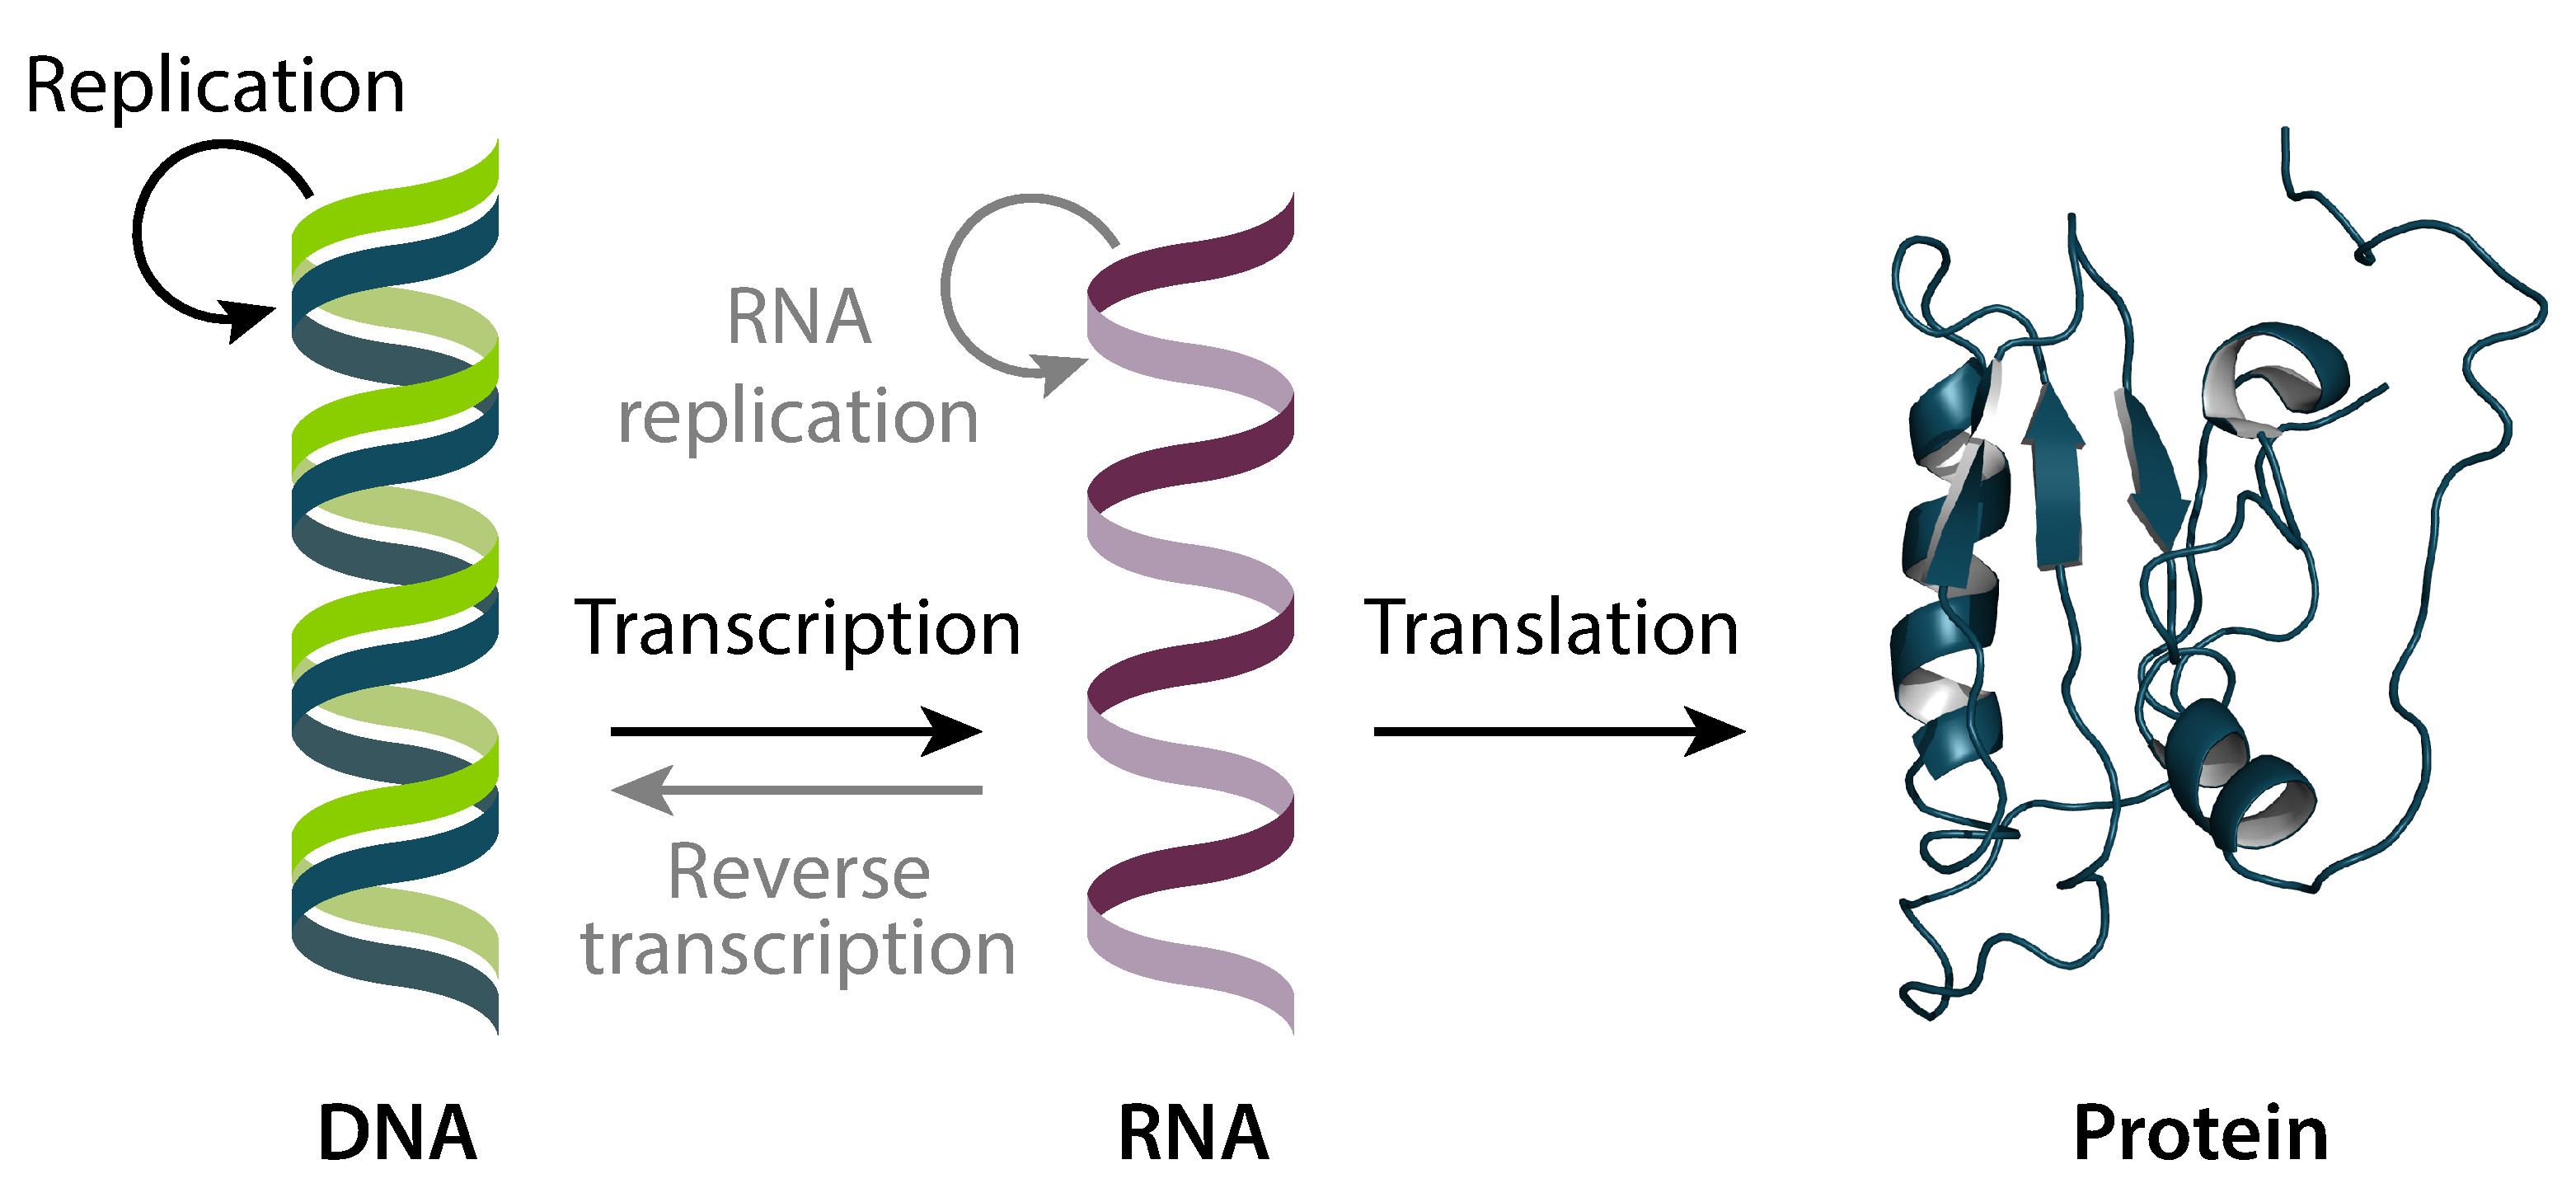
\includegraphics[width=1\linewidth]{figures/central_dogma.pdf}
    \caption{\textbf{Central dogma of molecular biology.} The central dogma of molecular biology states that Deoxiribonucleic Acid (\gls{dna}) replicates itself into more \gls{dna} molecules and it is also transcribed into Ribonucleic Acid (\gls{rna}), which is then translated into proteins. These processes, illustrated with black arrows, constitute the core of the central dogma of molecular biology and the most common flow of \gls{geneexpression}. This dogma has been expanded since its postulation (grey arrows), incorporating processes such as \gls{rna} replication, used by \gls{rna} viruses like poliovirus. Additionally, the Human Immunodeficiency Virus (HIV) utilizes reverse transcription to convert its \gls{rna} genome into \gls{dna}, which is then integrated into the host genome.}
    \label{fig:chapter1:central_dogma}
\end{figure}

\begin{figure}[tbh]
    \centering
    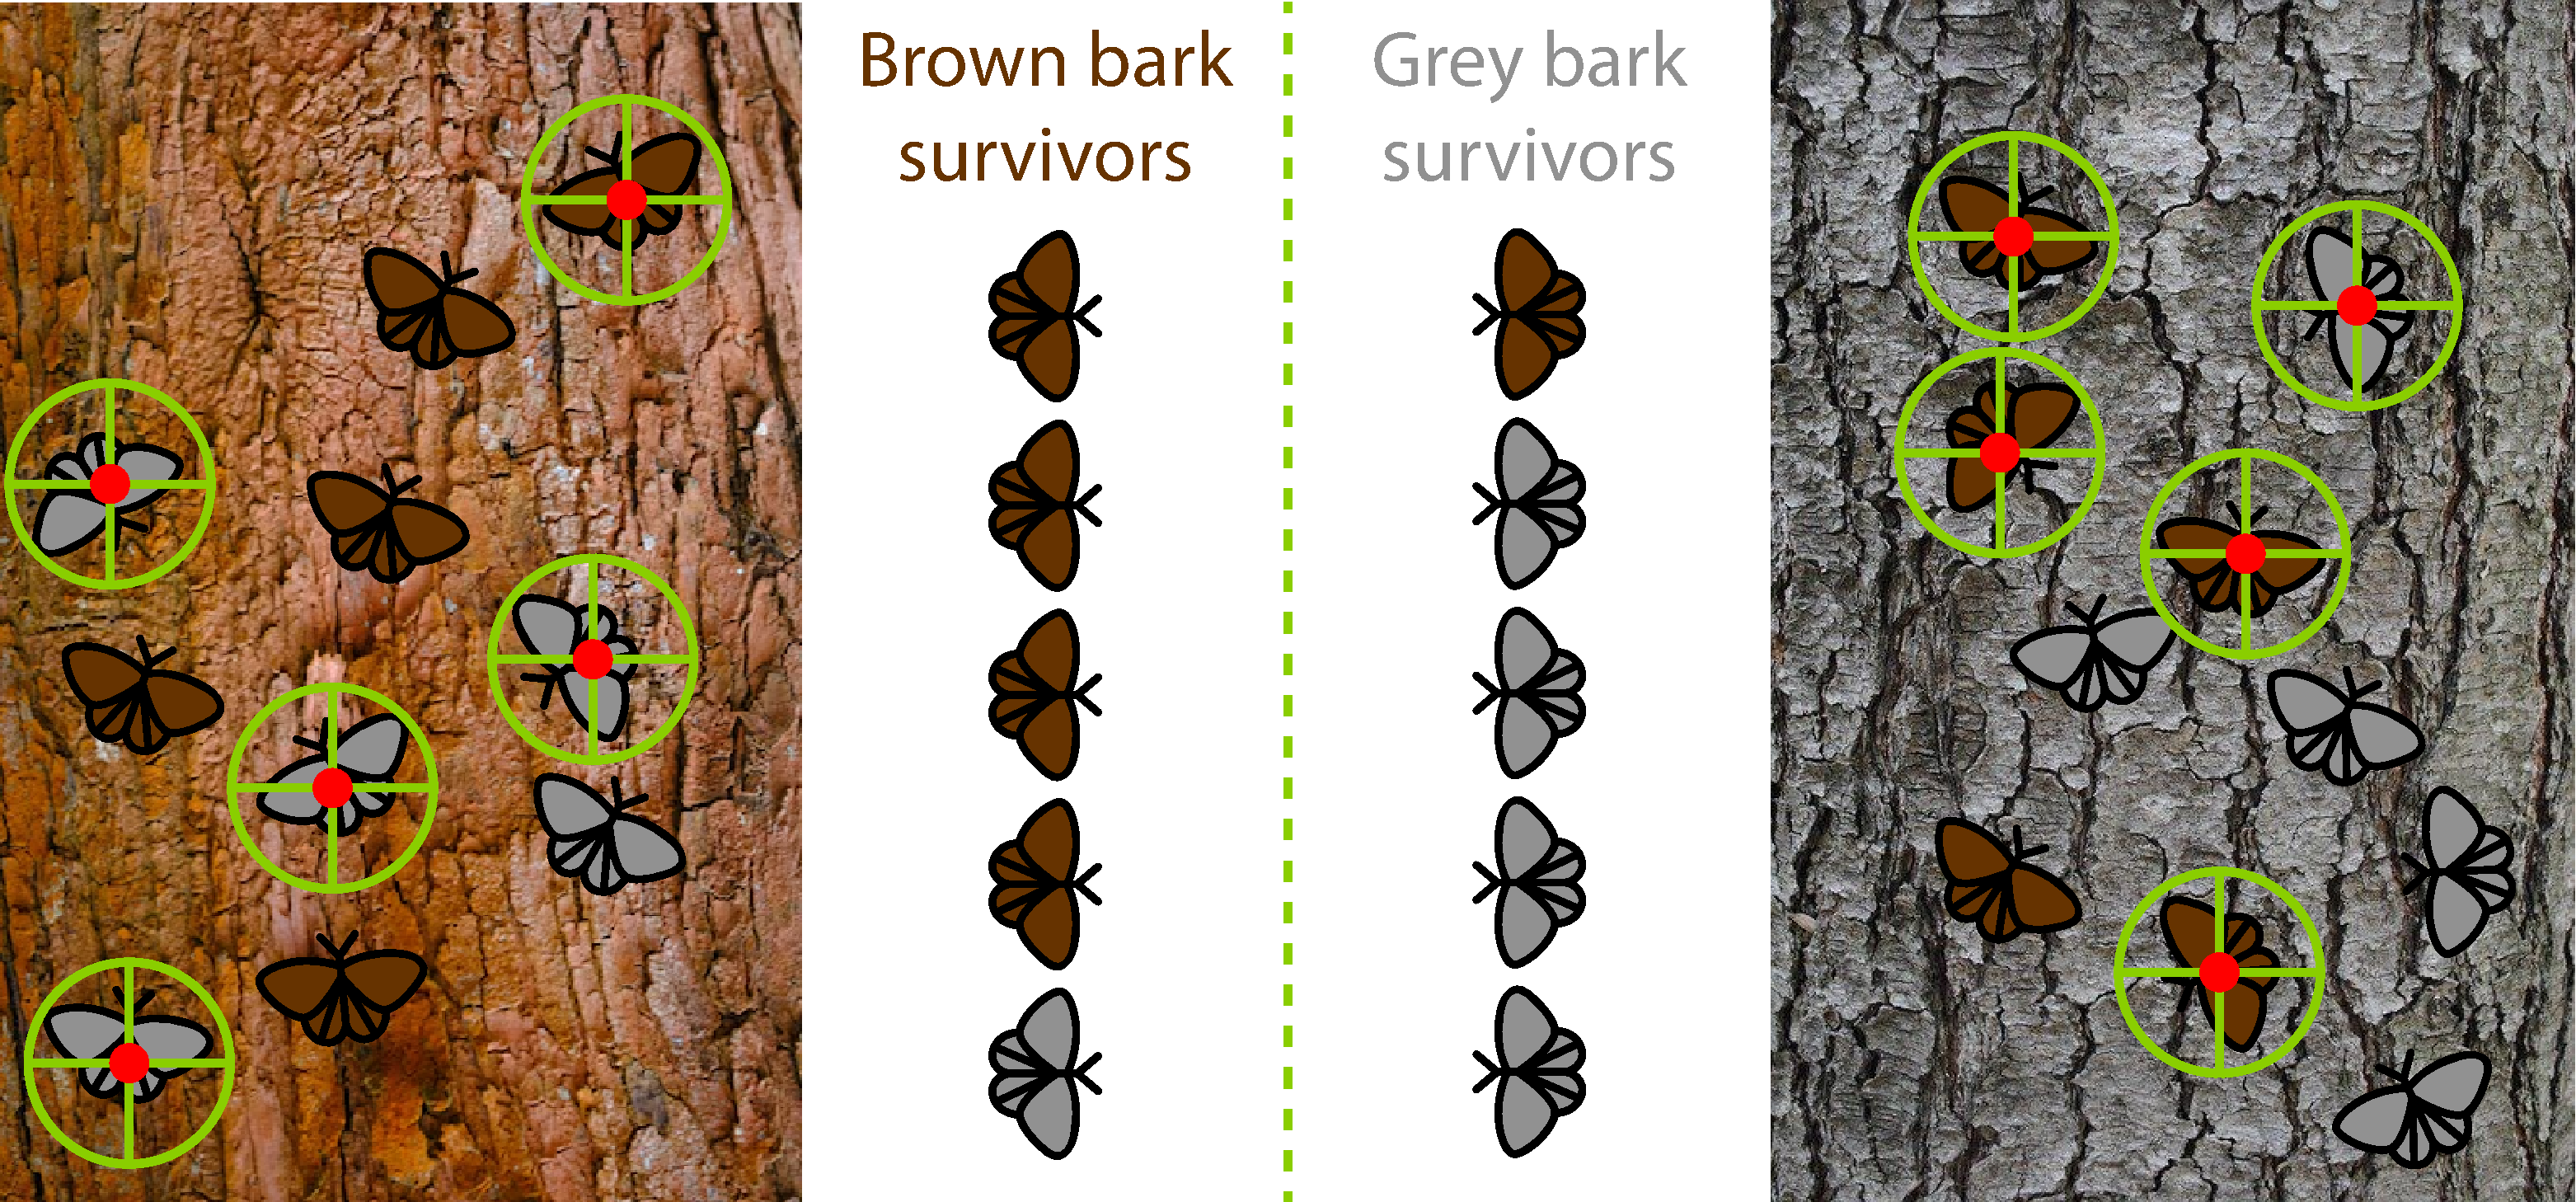
\includegraphics[width=1\linewidth]{figures/evolution_selection.pdf}
    \caption{\textbf{Evolutionary selection in different environments.} A population of moths with two different colours can be differentially selected depending on the environment. In this example, the moths are placed in trees with brown and a gray barks. In the brown bark tree, the gray moths are more visible to predators and are hunted in larger numbers that brown moths, and vice-versa. This results in differential survival rates, which will condition the traits for successful moth generations, selected for higher survival on a given bark colour.}
    \label{fig:chapter1:selection}
\end{figure}


Proteins, as a family of molecules present in living organisms, were formally described in the 19\textsuperscript{th} century \cite{natural_history_museum_library_sur_1838, hartley_origin_1951}. Later, they were characterised as a polypeptide chain \cite{dill_dominant_1990, gutte_peptides_1995}; their \gls{secondarystructure} and stabilisation by \glspl{hydrogenbond} were also described \cite{astbury_molecular_1931, pauling_atomic_1951, pauling_structure_1951}, and the use of \gls{xraycrystallography} crystallography in the 1950s enabled the first elucidation of protein \gls{tertiarystructure} \cite{kendrew_three-dimensional_1958, perutz_structure_1960}. In these early models of tertiary structure, it is noted that some regions are more difficult to elucidate, as quoted: ``If we attempt to trace a single continuous chain throughout the model, we soon run into difficulties and ambiguities, because we must follow it around corners, and it is precisely at corners that the chain must lose the tightly packed configuration which alone makes it visible at this resolution'' \cite{kendrew_three-dimensional_1958}. Even under the cold, dehydrated, and clearly non-native conditions to which proteins are subjected for \gls{xraycrystallography} crystallography \cite{fenwick_integrated_2014}, this was an early observation of protein \gls{dynamics} in structured proteins, illustrated by the spread location of \glspl{electron} in the molecule and consequent low resolution of the elucidated structure.

Protein \gls{dynamics} refer to the various motions and conformational changes that proteins undergo in their functional states. These encompass diverse ranges of motion, from atomic fluctuations and loop movements to large \gls{proteindomain} rearrangements, and time scales from pico-seconds to seconds. Many proteins contain intrinsically \glspl{proteindisorder} regions (\glspl{idr}) or are entirely intrinsically \glspl{proteindisorder} proteins (\glspl{idp}) \cite{tompa_intrinsically_2002, aspromonte_disprot_2024}. Unlike structured proteins, which have a well-defined three-dimensional structure, \glspl{idr} and \glspl{idp} lack a stable tertiary structure under \gls{physiologicalconditions}. These \glspl{proteindisorder} regions feature higher \gls{flexibility}, the ability to adopt diverse \glspl{conformation}, and often play a crucial role in a protein's function, such as \gls{ligand} binding. \Gls{proteindisorder} can also be transient and change according to its environment, such as in fold-upon-binding regions \cite{tsai_folding_1999, wright_linking_2009, fuxreiter_fold_2019}, which only adopt a defined structure during binding processes.

The elucidation of protein tertiary structures with \gls{xraycrystallography} crystallography drove the creation of the Protein Data Bank (PDB) \cite{berman_protein_2012} and nearly caused early research on protein \gls{proteindisorder} and \gls{dynamics} \cite{pauling_theory_1940, jirgensons_classification_1966} to be overshadowed by the determination of defined \glspl{proteinstructure} \cite{bondos_roles_2021}. Since then, protein science has gradually moved its views of \gls{proteinstructure} towards more dynamic models. The once universally accepted lock and key model for enzyme-substrate binding \cite{fischer_einfluss_1894} has transitioned into more dynamic binding models. Once such model is the induced fit model \cite{koshland_application_1958, vasella_glycosidase_2002}, in which the binding site changes \gls{conformation} to fit the substrate or a \glspl{proteindisorder} region folds upon binding \cite{tsai_folding_1999, bonetti_analyzing_2017, delaforge_deciphering_2018, bonetti_how_2018, fuxreiter_fold_2019, robustelli_mechanism_2020}. The other model is the conformational selection model \cite{tsai_structured_2001}, which states that all protein \glspl{conformation} exist in an equilibrium in its unbound state, even the bound \gls{conformation}, and the \gls{ligand} selectively binds to the ones with higher affinity \cite{vogt_conformational_2013, vogt_essential_2014}. 

The discovery of allosterism, the regulation of protein activity by binding to a different region than the active site, showed that such conformational changes can also be mediated by interactions in distant regions of a protein \cite{monod_general_1961, monod_nature_1965}. For example, the kinesin protein, responsible for processes such as intracellular transport, signal transduction, and chromosome movement during cell division, was observed to actively transport vesicles along cell microtubules in a similar motion as how humans walk \cite{vale_molecular_2003, endow_kinesins_2010}. Another example is the discovery of the revolver-like rotation in ATP (Adenosine triphosphate) synthases as a crucial part in transforming a \gls{proton} gradient into energy in the form of ATP \cite{noji_direct_1997}. This is a molecule that acts as the proteins' energy currency which can be ``spent'', hydrolised into ADP (Adenosine diphosphate), for processes that require energy, such as the previously mentioned ``walk'' of the kinesin protein (\figref{fig:chapter1:atp_adp}). Eventually, long-forgotten studies on protein \gls{proteindisorder} regained attention and the dynamic nature of proteins regained relevance.

\begin{figure}[tbh!]
    \centering
    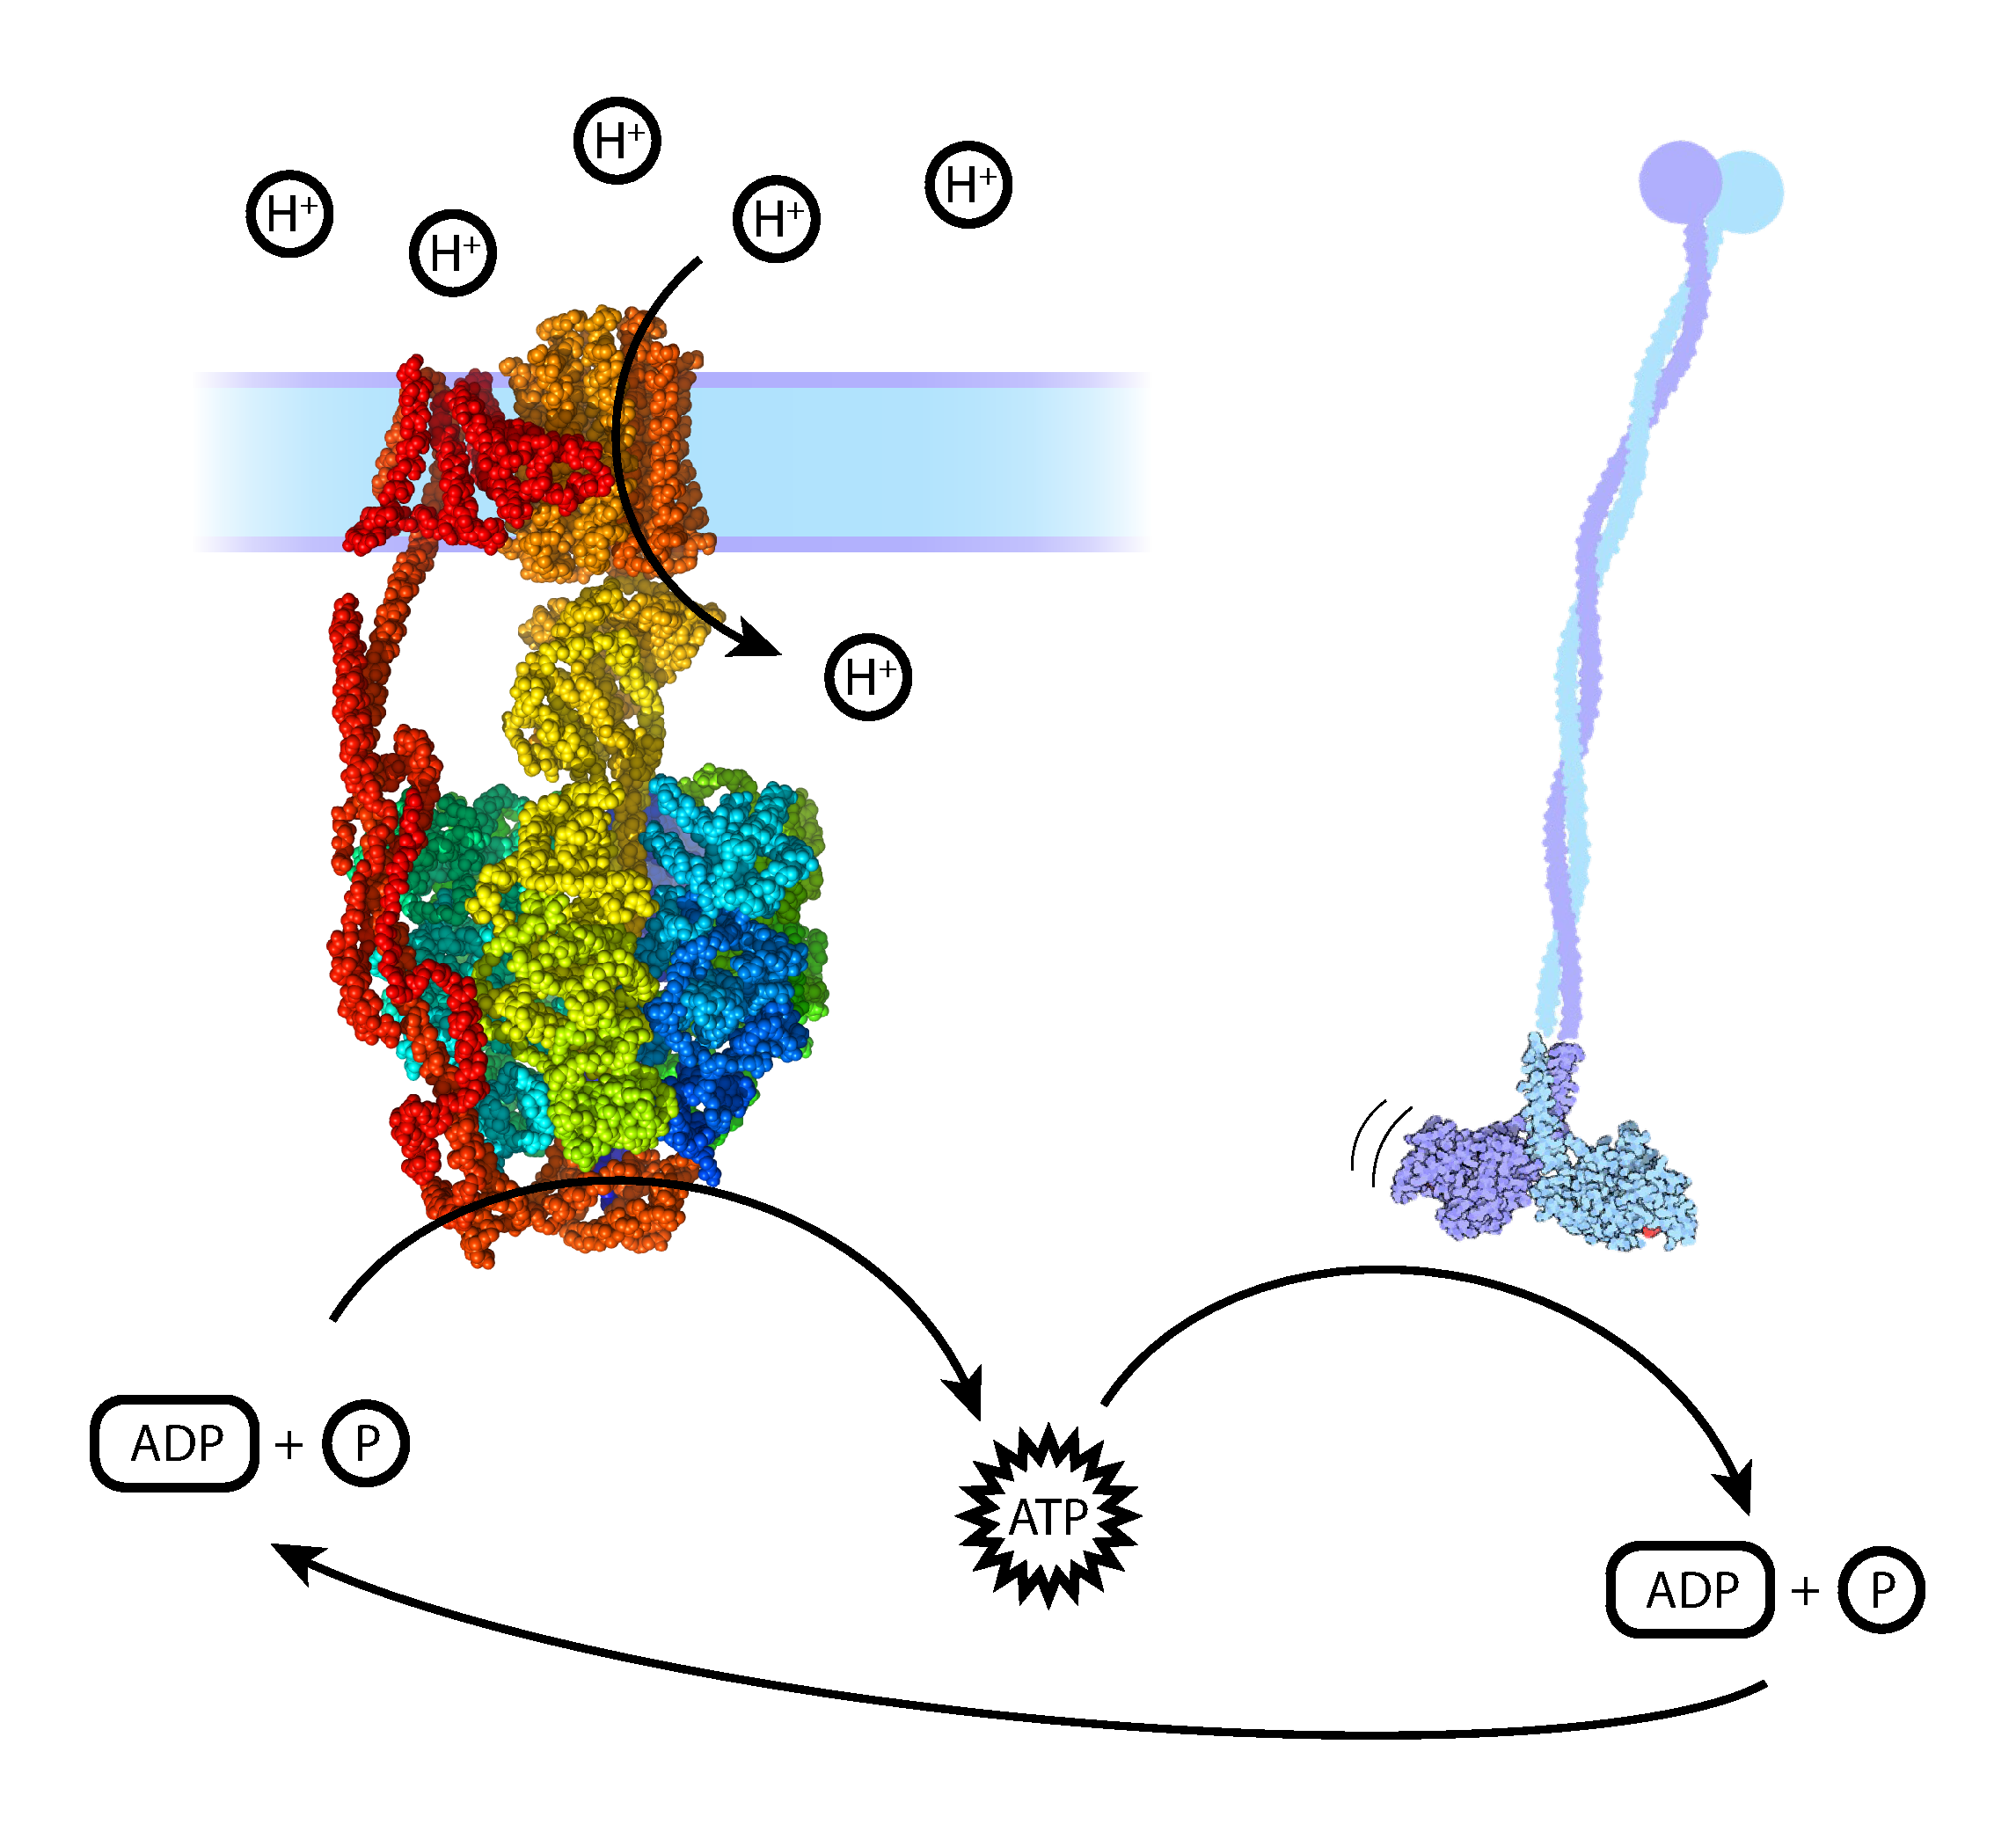
\includegraphics[width=0.8\linewidth]{figures/atp_adp_usage.pdf}
    \caption{\textbf{Synthesis and hydrolisation of ATP.} Mitochondrial ATP synthase (left, PDB-ID 5ARE) uses the \gls{proton} gradient and transport to synthesise ATP from ADP and a phosphate group. The chemical bond that incorporates the new phosphate group is energetically rich, making ATP the cell's energetic currency. This energy can be released through hydrolysis and used for active (i.e., energy-consuming) processes, such as the ``walk'' of the kinesin protein (right, image URL: \url{https://cdn.rcsb.org/pdb101/motm/64/3kin-composite.gif}).}
    \label{fig:chapter1:atp_adp}
\end{figure}


% \section{Protein Structure Fundamentals}
\section{Protein Structural Organisation}

Protein motion is defined by simultaneous effects of endogenous and exogenous factors, some of which we will elaborate in this chapter. One of these is a protein's own structure, which determines its degrees of freedom and stability. The description of \gls{proteinstructure} is hierarchically organised, with each subsequent level describing larger scales of \gls{proteinstructure}. The \gls{primarystructure} of a protein, a protein's lowest structural level, describes it as a polypeptide sequence, a chain of \glspl{aminoacid} bound with peptide bonds. This chain is generally formed by a combination of 20 \glspl{aminoacid} (though non-standard \glspl{aminoacid} lengthen the list), each of them featuring different intrinsic properties (\textit{e.g.} polar, aromatic, hydrophobic...) \cite{neilan_amino_2003}. The peptide bond keeping these \glspl{aminoacid} together is a special kind of bond, as it results in a plane which restricts the trajectory of the polypeptide chain (\figref{fig:chapter1:peptide_bond}), resembling the interleaved rigid-motile-rigid pattern featured in the links of a metal chain. These planes make $\text{C}_{\alpha}$ the only possible flexing point of an \gls{aminoacid} in a poly-peptide chain (besides small variation in $\omega$ angles), and two angles $\phi$ and $\psi$ are defined as the orientation of these planes with respect to $\text{C}_{\alpha}$. 

\begin{figure}[tbh]
    \centering
    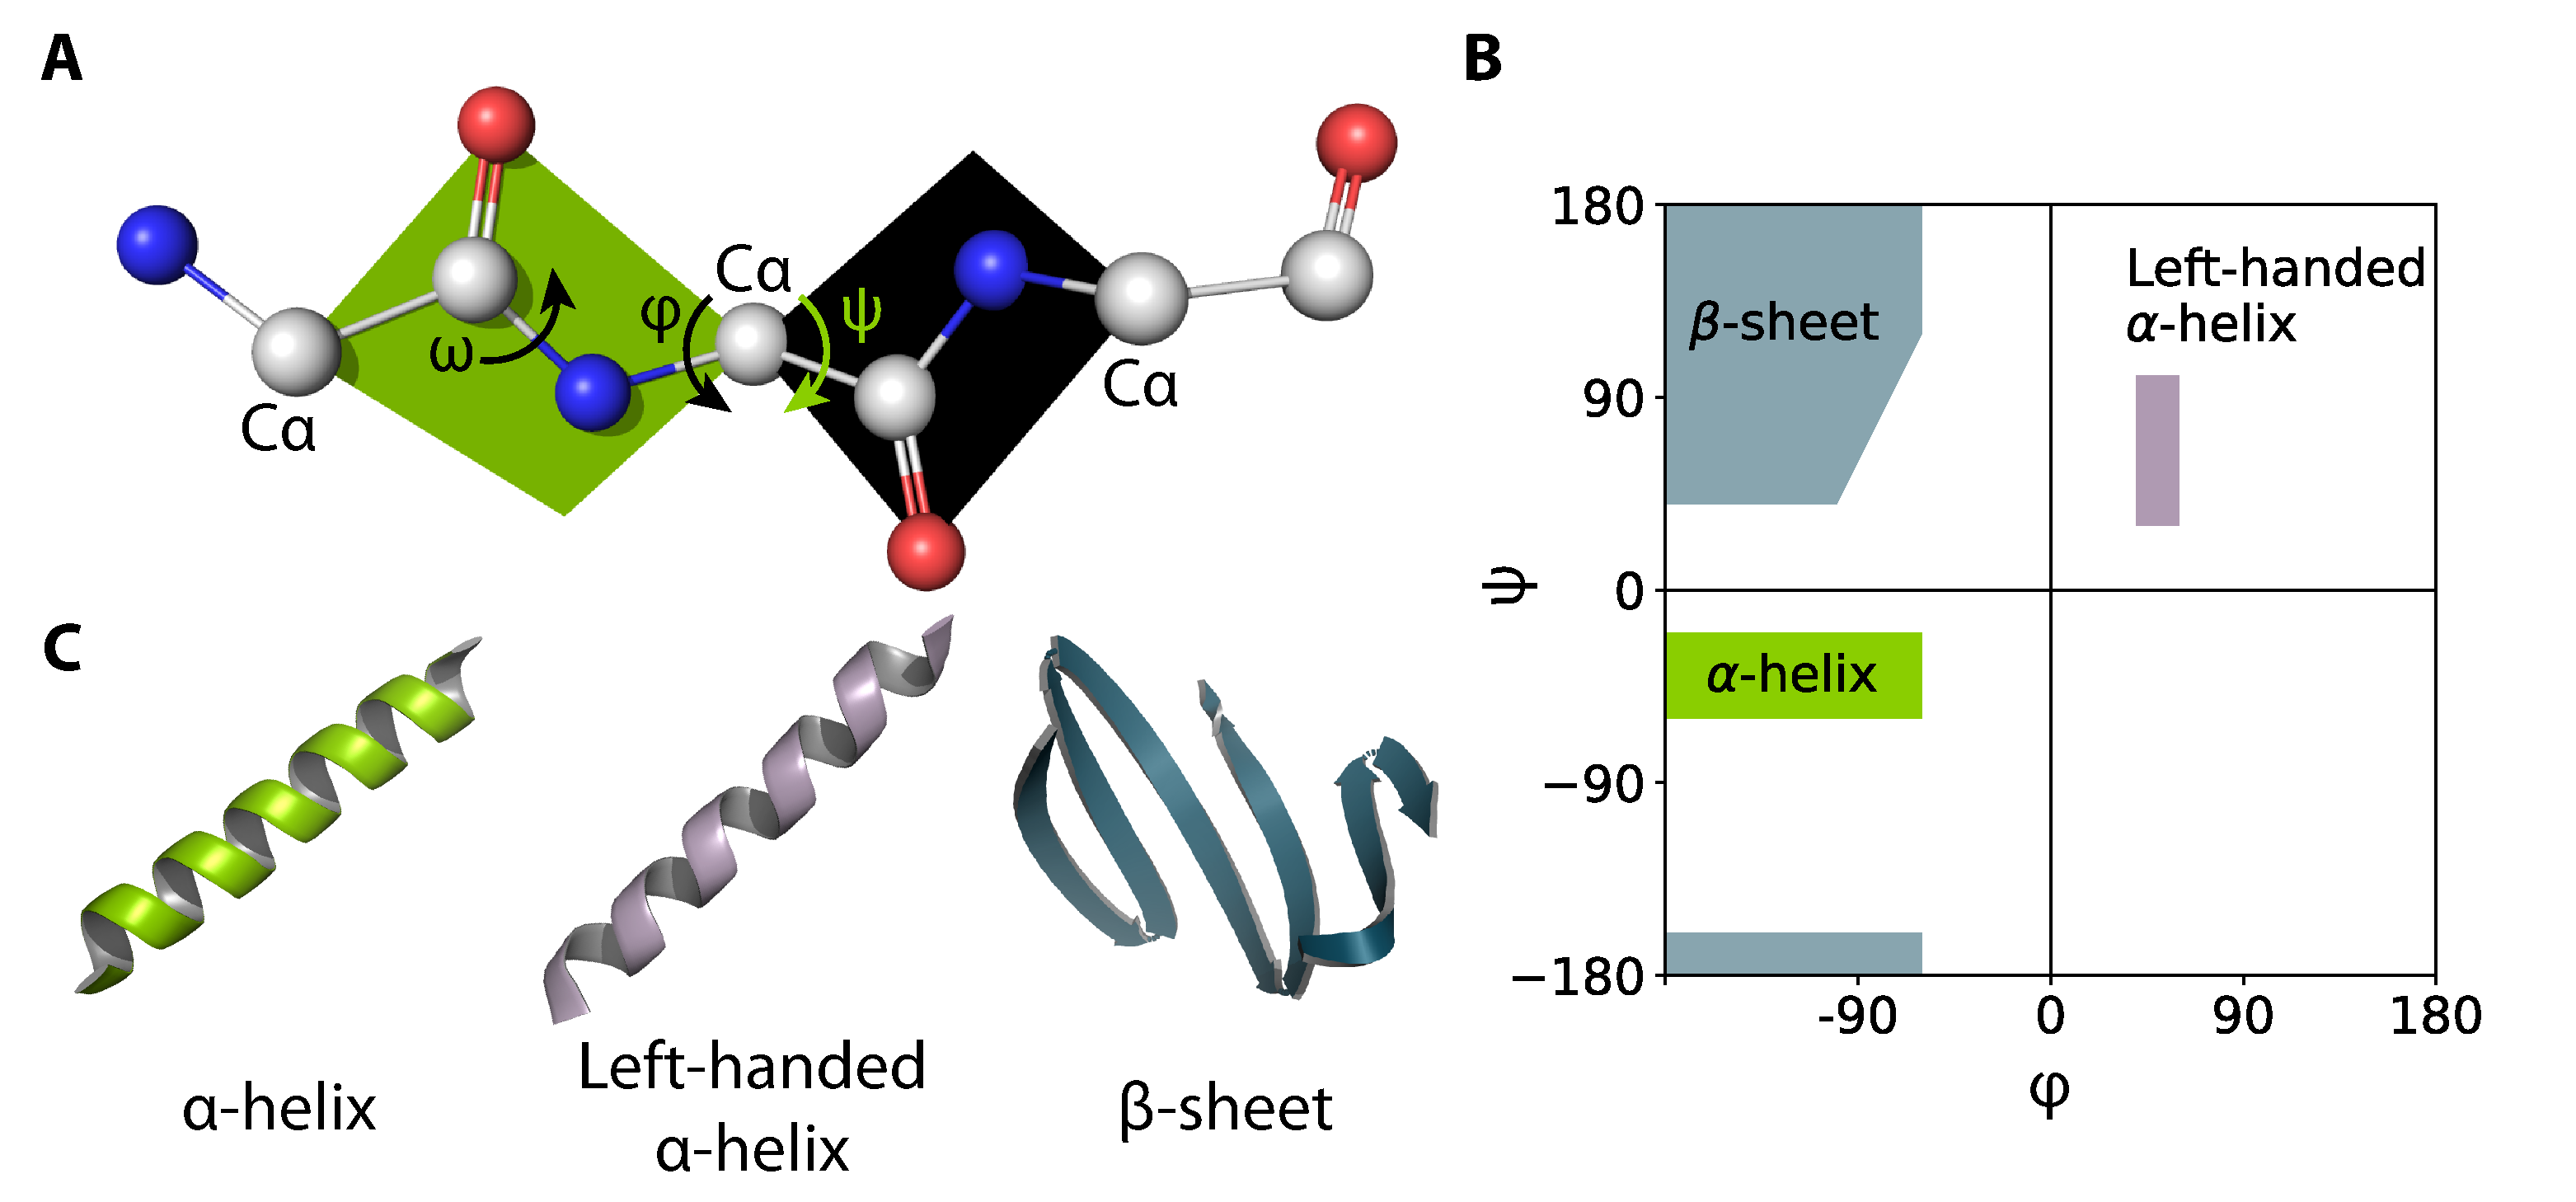
\includegraphics[width=1\linewidth]{figures/peptide_bond_rama.pdf}
    \caption{\textbf{Peptide bond, dihedral angles and their relation to secondary structure.} A) Section of a protein \gls{backbone} centered around the $\text{C}_{\alpha}$ of an \gls{aminoacid}. The peptide bonds between the amino (blue sphere) and the carboxyl (gray and red spheres) groups define a plane, with limited torsion, defined by the omega ($\omega$) angle. These planes' orientation respect to a $\text{C}_{\alpha}$ is described by the phi ($\phi$) and psi ($\psi$) angles. B) The $\phi$ and $\psi$ dihedral angles can be represented in a \gls{ramachandranplot}. This plot represents a torus (doughnut) space where areas can be delimited to represent different types of secondary structures. C) Visualisation of the common secondary structures represented in the \gls{ramachandranplot}.}
    \label{fig:chapter1:peptide_bond}
\end{figure}
 

% Every $\phi$ and $\psi$ angle in every \gls{aminoacid} of the protein determines a sequential path that defines the overall shape of the protein. If a protein's full conformational space (\textit{i.e.} every possible combination of $\phi$ and $\psi$ angles for every \gls{aminoacid}) was explored for a given protein local environment (\textit{e.g.} \gls{physiologicalconditions}, no binding partner, 37$^\circ\mathrm{C}$), a continuum of energy levels could be represented as a multi-dimensional energy surface or landscape \cite{dill_protein_2008}. These energy levels are measured by the \gls{gibbsfreeenergy} \cite{yang_free_2013}, defined as: 


% \begin{equation}
% \label{eq:GibbsFreeEnergy}
% G = H - TS
% \end{equation}

% where \( G \) is the \gls{gibbsfreeenergy}, \( H \) is the \gls{enthalpy} (which represents the total heat content of the system), \( T \) is the absolute temperature (in Kelvin), and \( S \) is the \gls{entropy} (which measures the disorder or randomness in the system). Every change in $\phi$ and $\psi$ angles results in a displacement in the landscape, which carries a change in \gls{entropy} and \gls{enthalpy} and thereby generally a change in \gls{gibbsfreeenergy}. The change of energy associated to change in protein fold is described as follows:

% \begin{equation}
% \label{eq:GibbsFreeEnergyChange}
% \Delta G = \Delta H - T \Delta S
% \end{equation}

% where \(\Delta G\) is the change in \gls{gibbsfreeenergy}, \(\Delta H\) is the change in \gls{enthalpy}, \(T\) is the absolute temperature, and \(\Delta S\) is the change in \gls{entropy} upon folding. At constant temperature (\textit{e.g.} in human \gls{physiologicalconditions}) the \gls{gibbsfreeenergy} is a function of a fold's \gls{enthalpy} and \gls{entropy}. In the context of protein fold, \gls{enthalpy} reduction occurs in events such as the formation of covalent and \glspl{hydrogenbond}, the exclusion of solvent from the system by hydrophobic packing, or aromatic rings stacking \cite{santiago_relation_2010, liu_protein_2012}. \Gls{entropy} refers to the disorder of the system, which is decreased by events such as the exposure of hydrophilic \glspl{aminoacid} to solvent (thereby burying hydrophobic \glspl{aminoacid} in the protein core) freeing the orientation of a protein's surrounding solvent, or the binding to a \gls{ligand} \cite{bonetti_analyzing_2017, bonetti_how_2018}. Proteins aim to reduce their \gls{gibbsfreeenergy}, navigating the energy landscape to reach a \gls{conformation} that represents an energy minimum (\figref{fig:chapter1:landscape}).

\subsection{Thermodynamics view of protein conformation}
Every \(\phi\) and \(\psi\) angle in every amino acid of a protein defines a sequential path that contributes to the overall shape of the protein. The full conformational space of a protein (\textit{i.e.} every possible combination of \(\phi\) and \(\psi\) angles for every amino acid) represents a complex energy landscape that includes both enthalpic and entropic contributions. If we consider a given protein's local environment (\textit{e.g.} physiological conditions, no binding partner, 37°C), this energy landscape can be visualised as a multi-dimensional surface where each point corresponds to a different conformation with a specific Gibbs free energy \cite{dill_protein_2008}.

The Gibbs free energy (\(G\)) of a protein conformation is defined by the equation:

\begin{equation}
\label{eq:GibbsFreeEnergy}
G = H - TS
\end{equation}

where \(H\) is the enthalpy (the total heat content of the system), \(T\) is the absolute temperature in Kelvin, and \(S\) is the entropy (which measures the disorder or randomness in the system) \cite{yang_free_2013}. 

The entropic contribution to the Gibbs free energy, which is related to the number of microstates adopted by the system, including surrounding water molecules, is difficult to capture. For example, the Gibbs free energy of proteins that adopt a single unique conformation with minimal internal entropy will decrease during the folding process, with the reduction in entropy compensated by enthalpic factors such as hydrogen bonding. Therefore, their Gibbs free energy can be approximated to their enthalpy, such as:

\begin{equation}
\label{eq:GibbsFreeEnergy_only_enthalpy}
G \approx H
\end{equation}


% Considering a folded protein that can only adopt a single conformation, such a protein would essentially have zero configurational entropy, as the system is restricted to a single microstate. Without the ability to explore multiple conformations, the protein lacks the structural variability that contributes to entropy. Some other forms of entropy could still have minor contributions on the system, such as solvent-related entropy (\textit{e.g.} changes in the orientation of water molecules surrounding the protein) or vibrational entropy (\textit{e.g.} compression and stretching of chemical bonds). Nevertheless, the overall entropy of the system would be significantly reduced with no contribution from conformational freedom. Therefore, its Gibbs free energy can be approximated to its enthalpy, such as:

% \begin{equation}
% \label{eq:GibbsFreeEnergy_only_enthalpy}
% G \approx H
% \end{equation}

Changes in this system's Gibbs free energy are therefore mostly due to changes in the system's enthalpy. Enthalplic changes can still occur in fixed conformations, for example by the formation of chemical bonds or by the post-translational modification of residues, described by:

\begin{equation}
\label{eq:GibbsFreeEnergy_only_enthalpy_change}
\Delta G \approx \Delta H
\end{equation}

where \(\Delta G\) is the change in Gibbs free energy, \(\Delta H\) is the change in enthalpy. Note that the approximation, rather than equality, in equations \ref{eq:GibbsFreeEnergy_only_enthalpy} and \ref{eq:GibbsFreeEnergy_only_enthalpy_change} allocates for the small contributions to the system of non-configurational entropies.

On the other hand, the thermodynamically most stable state of intrinsically disordered proteins, which do not have a unique fold, will be rather driven by entropic effects and multiple conformations. The overall role of water molecules in this energy landscape is very difficult to capture and at the moment understudied.

For proteins with flexible structures, changes in \(\phi\) and \(\psi\) angles lead to different protein conformations, which are associated with changes in both enthalpy and entropy, thereby altering the Gibbs free energy of the system. The change in Gibbs free energy associated with a transition between different protein conformations, such as folding, is described by:

\begin{equation}
\label{eq:GibbsFreeEnergyChange}
\Delta G = \Delta H - T \Delta S
\end{equation}

where \(\Delta G\) is the change in Gibbs free energy, \(\Delta H\) is the change in enthalpy, and \(\Delta S\) is the change in entropy upon folding or unfolding. At constant temperature (e.g. in human physiological conditions), the Gibbs free energy reflects the balance between enthalpy and entropy changes as the protein explores its conformational space.

\subsection{Thermodynamics of protein folding}
During protein folding, various interactions like hydrogen bonds, hydrophobic effects, and van der Waals forces contribute to a reduction in enthalpy by stabilising specific conformations \cite{santiago_relation_2010, liu_protein_2012}. Simultaneously, the folding process reduces the protein’s entropy due to the decreased conformational freedom of the polypeptide chain. However, this entropic cost can be offset by an increase in the entropy of the surrounding solvent as hydrophobic groups are buried away from water, freeing water molecules that were previously structured around these groups, oriented in a polar manner \cite{bonetti_analyzing_2017, bonetti_how_2018}.

Proteins naturally fold to minimise their Gibbs free energy, finding a conformation that represents an energy minimum, which is the most stable state under given conditions (\figref{fig:chapter1:landscape}).


\begin{figure}[tbh!]
    \centering
    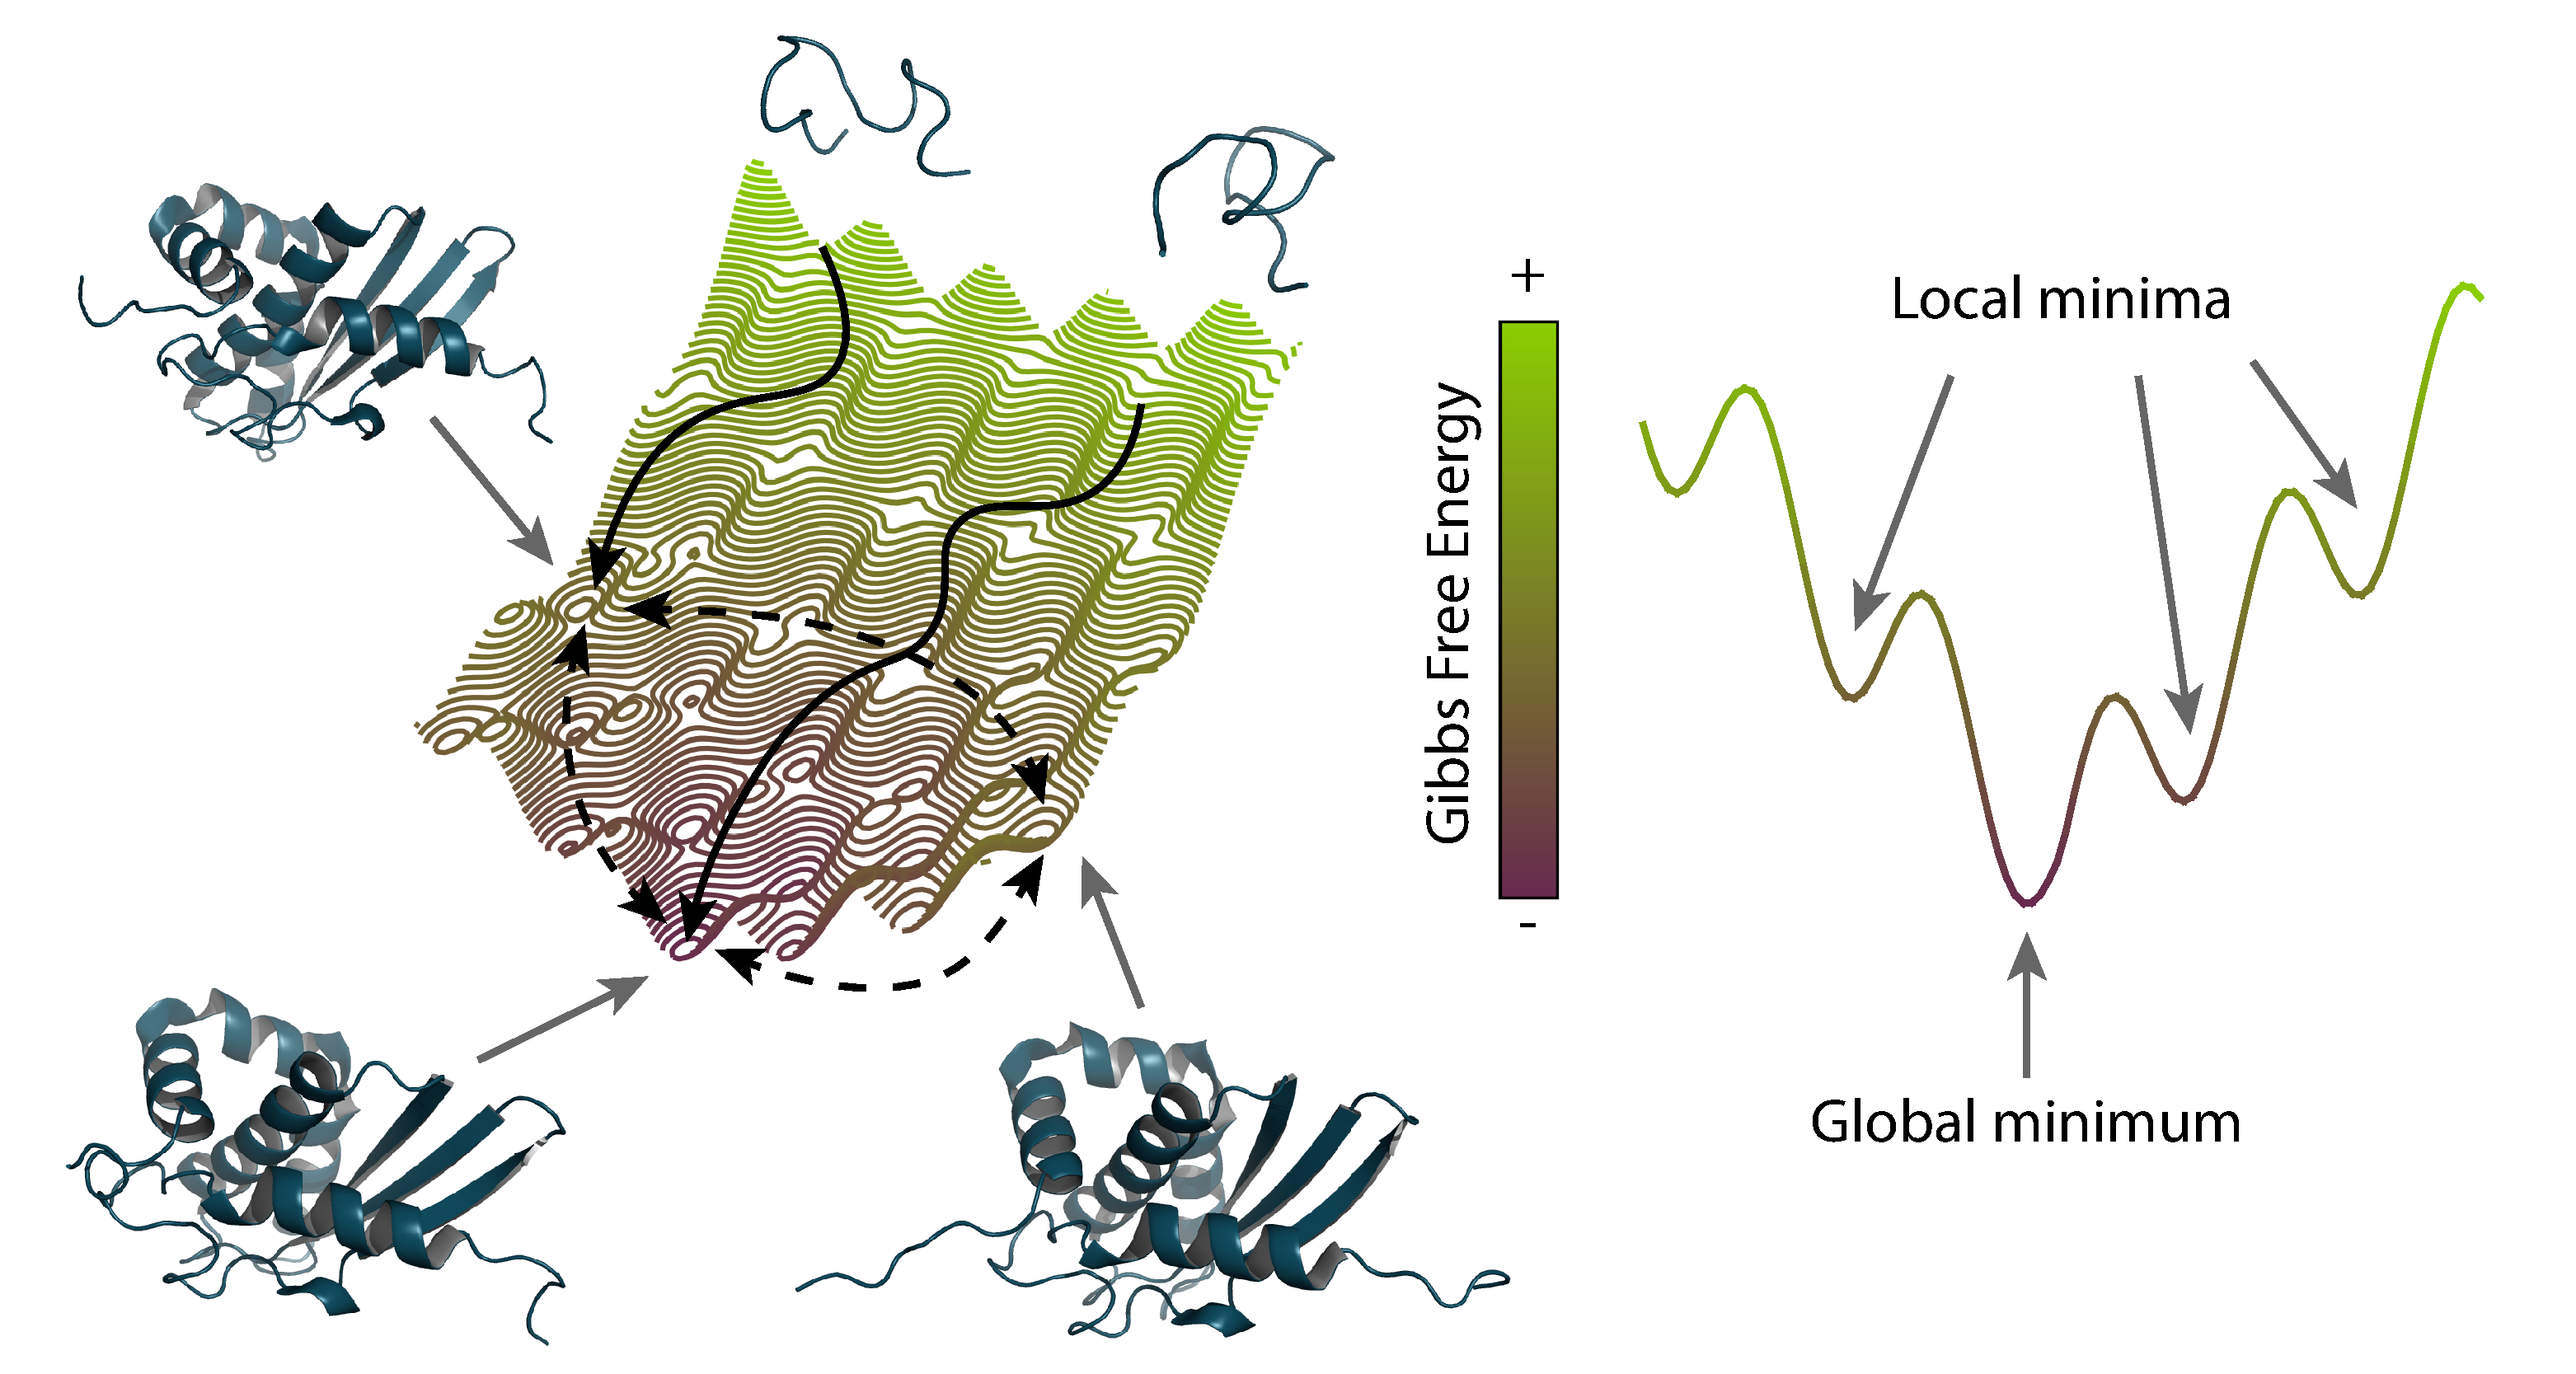
\includegraphics[width=1\linewidth]{figures/energy_landscape.pdf}
    \caption{\textbf{\gls{gibbsfreeenergy} landscape in 3D and 2D representations.} A protein acquires a fold by finding lower-energy states on the \gls{gibbsfreeenergy} landscape. On the left, two different paths to fold (solid black lines) are illustrated on a 3D representation of the landscape, where both paths reach an energy minimum state. The rightmost path reaches the global minimum, while the leftmost stays in a local minimum. These minima are more clearly visualised in the 2D representation on the right side of the figure. This landscape shows the thermodynamic stability of different \glspl{conformation} that lie in \glspl{localminima} energy states. Transitions between these conformations, such as moving from a local minimum to the global minimum, require overcoming energy barriers (peaks in the landscape), which is a kinetic process that depends on the rate at which these barriers can be crossed. PDB ID: 2M5H \cite{ouyang_solution_2013} (diverse conformers from the \gls{nmr} ensemble).}
    \label{fig:chapter1:landscape}
\end{figure}

The simplest spatial structural description of a protein is the secondary structure of its regions. Secondary structures are defined by their \gls{hydrogenbond} stabilisation patterns and their \glspl{aminoacid}' $\phi$ and $\psi$ dihedral angles (\figref{fig:chapter1:peptide_bond}). Proteins further reduce their \gls{gibbsfreeenergy} by folding and adopting their tertiary structure (\textit{i.e.} their overall monomeric \gls{conformation}). In some cases, proteins are composed of multiple sub-units or chains (\textit{e.g.} Mitochondrial ATP synthase in \figref{fig:chapter1:atp_adp}, coloured by chain). These proteins also feature a \gls{quaternarystructure}, which describes how these sub-units bind together to adopt a thermodynamically-favourable \gls{conformation}.

\subsection{The Folding Process}
The process followed by a protein to acquire a functional \gls{conformation} is called its folding process. This process occurs as a complex interaction of entropic and enthalpic elements, described in this section, such as solvent effects, presence of \gls{electrostaticinteractions}, or interaction with other proteins. These elements take place simultaneously and compete with or assist each other at different stages \cite{onuchic_theory_2004}. The effects of these elements can be permanent in a protein's final \gls{conformation} (\textit{e.g.} formation of \glspl{hydrogenbond} that define a secondary structure element, formation of disulphide bonds between cysteine \glspl{aminoacid}, appending post-translational modifications to the \glspl{aminoacid}, or the binding of sub-units in a multimeric protein), or be transient and employed to overcome an energy barrier and further descend in the \gls{gibbsfreeenergy} landscape (\textit{e.g.} binding of chaperones \cite{dandage_classification_2015, balchin_recent_2020, lu_energy_2021} or temporary co-factors \cite{wittung-stafshede_role_2002, wilson_role_2004, bushmarina_cofactor_2006}). A \gls{foldingpath} is defined as a result of these elements' interaction, which results in a descent in the \gls{gibbsfreeenergy} landscape to \glspl{conformation} with lower energy levels. As proteins adopt a conformation, even proteins that will later remain in a single unique conformation will experience a descent in Gibbs free energy during the folding process. These also experience entropic effects because they are not yet restricted to a single microstate during the folding process and can therefore transition between them. The number of allowed microstates narrows as the folding process progresses, in some cases up to a single conformation.


The folding of a protein can be divided into the acquisition of both local and global \glspl{conformation}. The local \gls{conformation} refers to the spatial arrangement of the protein’s \gls{aminoacid} sequence within short segments, including secondary structures and \glspl{foldon}. \Glspl{foldon} are regions of the protein that fold quasi-independently, with minimal \glspl{foldingfrustration} (i.e., their folding process does not significantly affect the folding of other regions) \cite{panchenko_foldons_1996, maity_protein_2005, englander_nature_2014}. The interactions between all elements of a protein’s local \gls{conformation} contribute to the formation of its global \gls{conformation}, which is the protein's overall three-dimensional structure at a given time.

Generally, the \gls{nativefold} of a protein is defined as the lowest energy point of this landscape under \gls{physiologicalconditions}. This landscape's topology is rugged funnel-shaped, biased towards the \gls{nativefold} \cite{onuchic_theory_2004}, with \glspl{localminima} that represent relatively stable \glspl{conformation} that a protein can adopt \cite{tsai_structured_2001} (\figref{fig:chapter1:landscape}). Later in this thesis, it will be posited that \gls{proteinstructure} is better explained as a continuum of allowed \glspl{conformation}.


\section{Experimental Study of Protein Motion}

\subsection{Molecular Biology and Microscopy Methods}

Different time scales and magnitudes of protein motions require different methods for their study (\figref{fig:chapter1:timescale}). At the largest magnitudes of motions, there is a variety of proteins capable of large molecular motions, essentially molecular motors responsible for large molecular motions \cite{schliwa_molecular_2003}. Some of these largest motions can be identified with creative molecular biology techniques, like the linking of larger and/or fluorescent molecules to mobile regions of a protein, in combination with \gls{microscopy}. These large protein motions are often responsible for crucial cellular processes, such as mitochondrial respiration with the previously mentioned ATP synthase (\figref{fig:chapter1:synthase_rotation}) \cite{noji_direct_1997, sambongi_mechanical_1999, hirono-hara_pause_2001}, transport of cargo in vesicles along microtubules with the hand-over-hand walk of Kinesins \cite{yildiz_kinesin_2004}, or the separation of chromosomes during cell division \cite{sawin_motor_1991, schliwa_molecular_2003}.

\begin{figure}[tbh!]
    \centering
    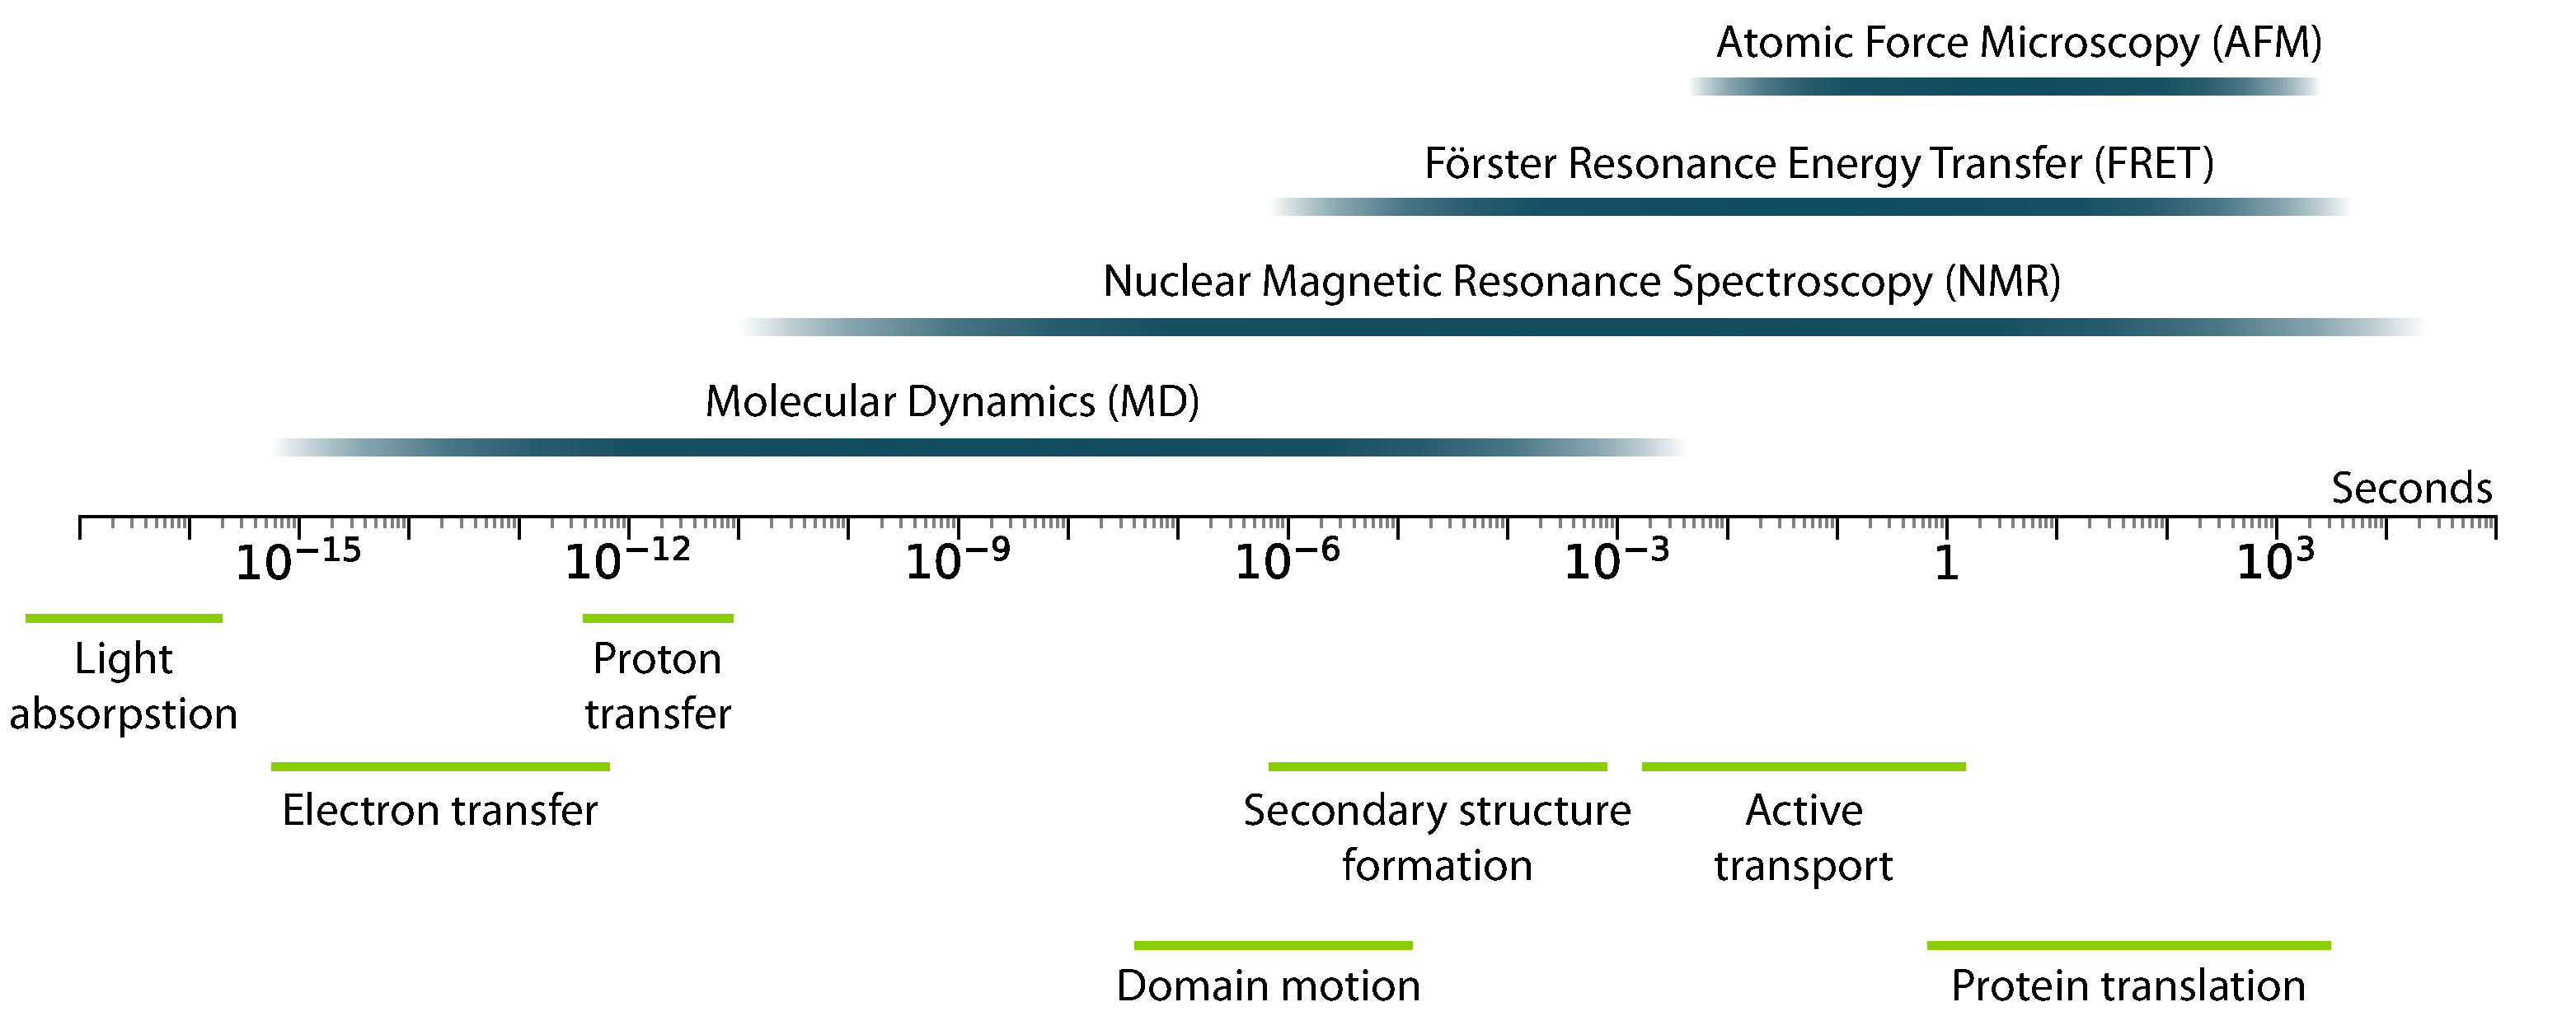
\includegraphics[width=1\linewidth]{figures/timescale_dynamics.pdf}
    \caption{\textbf{Time scale for protein \gls{dynamics} methods compared to physical and biological processes.} Diverse methods to study protein \gls{dynamics} (top) and their time resolution are illustrated with the time-scale of physical and biological processes (bottom). Adapted from Fig. 1 in \cite{ode_molecular_2012}).}
    \label{fig:chapter1:timescale}
\end{figure}

\begin{figure}[tbh!]
    \centering
    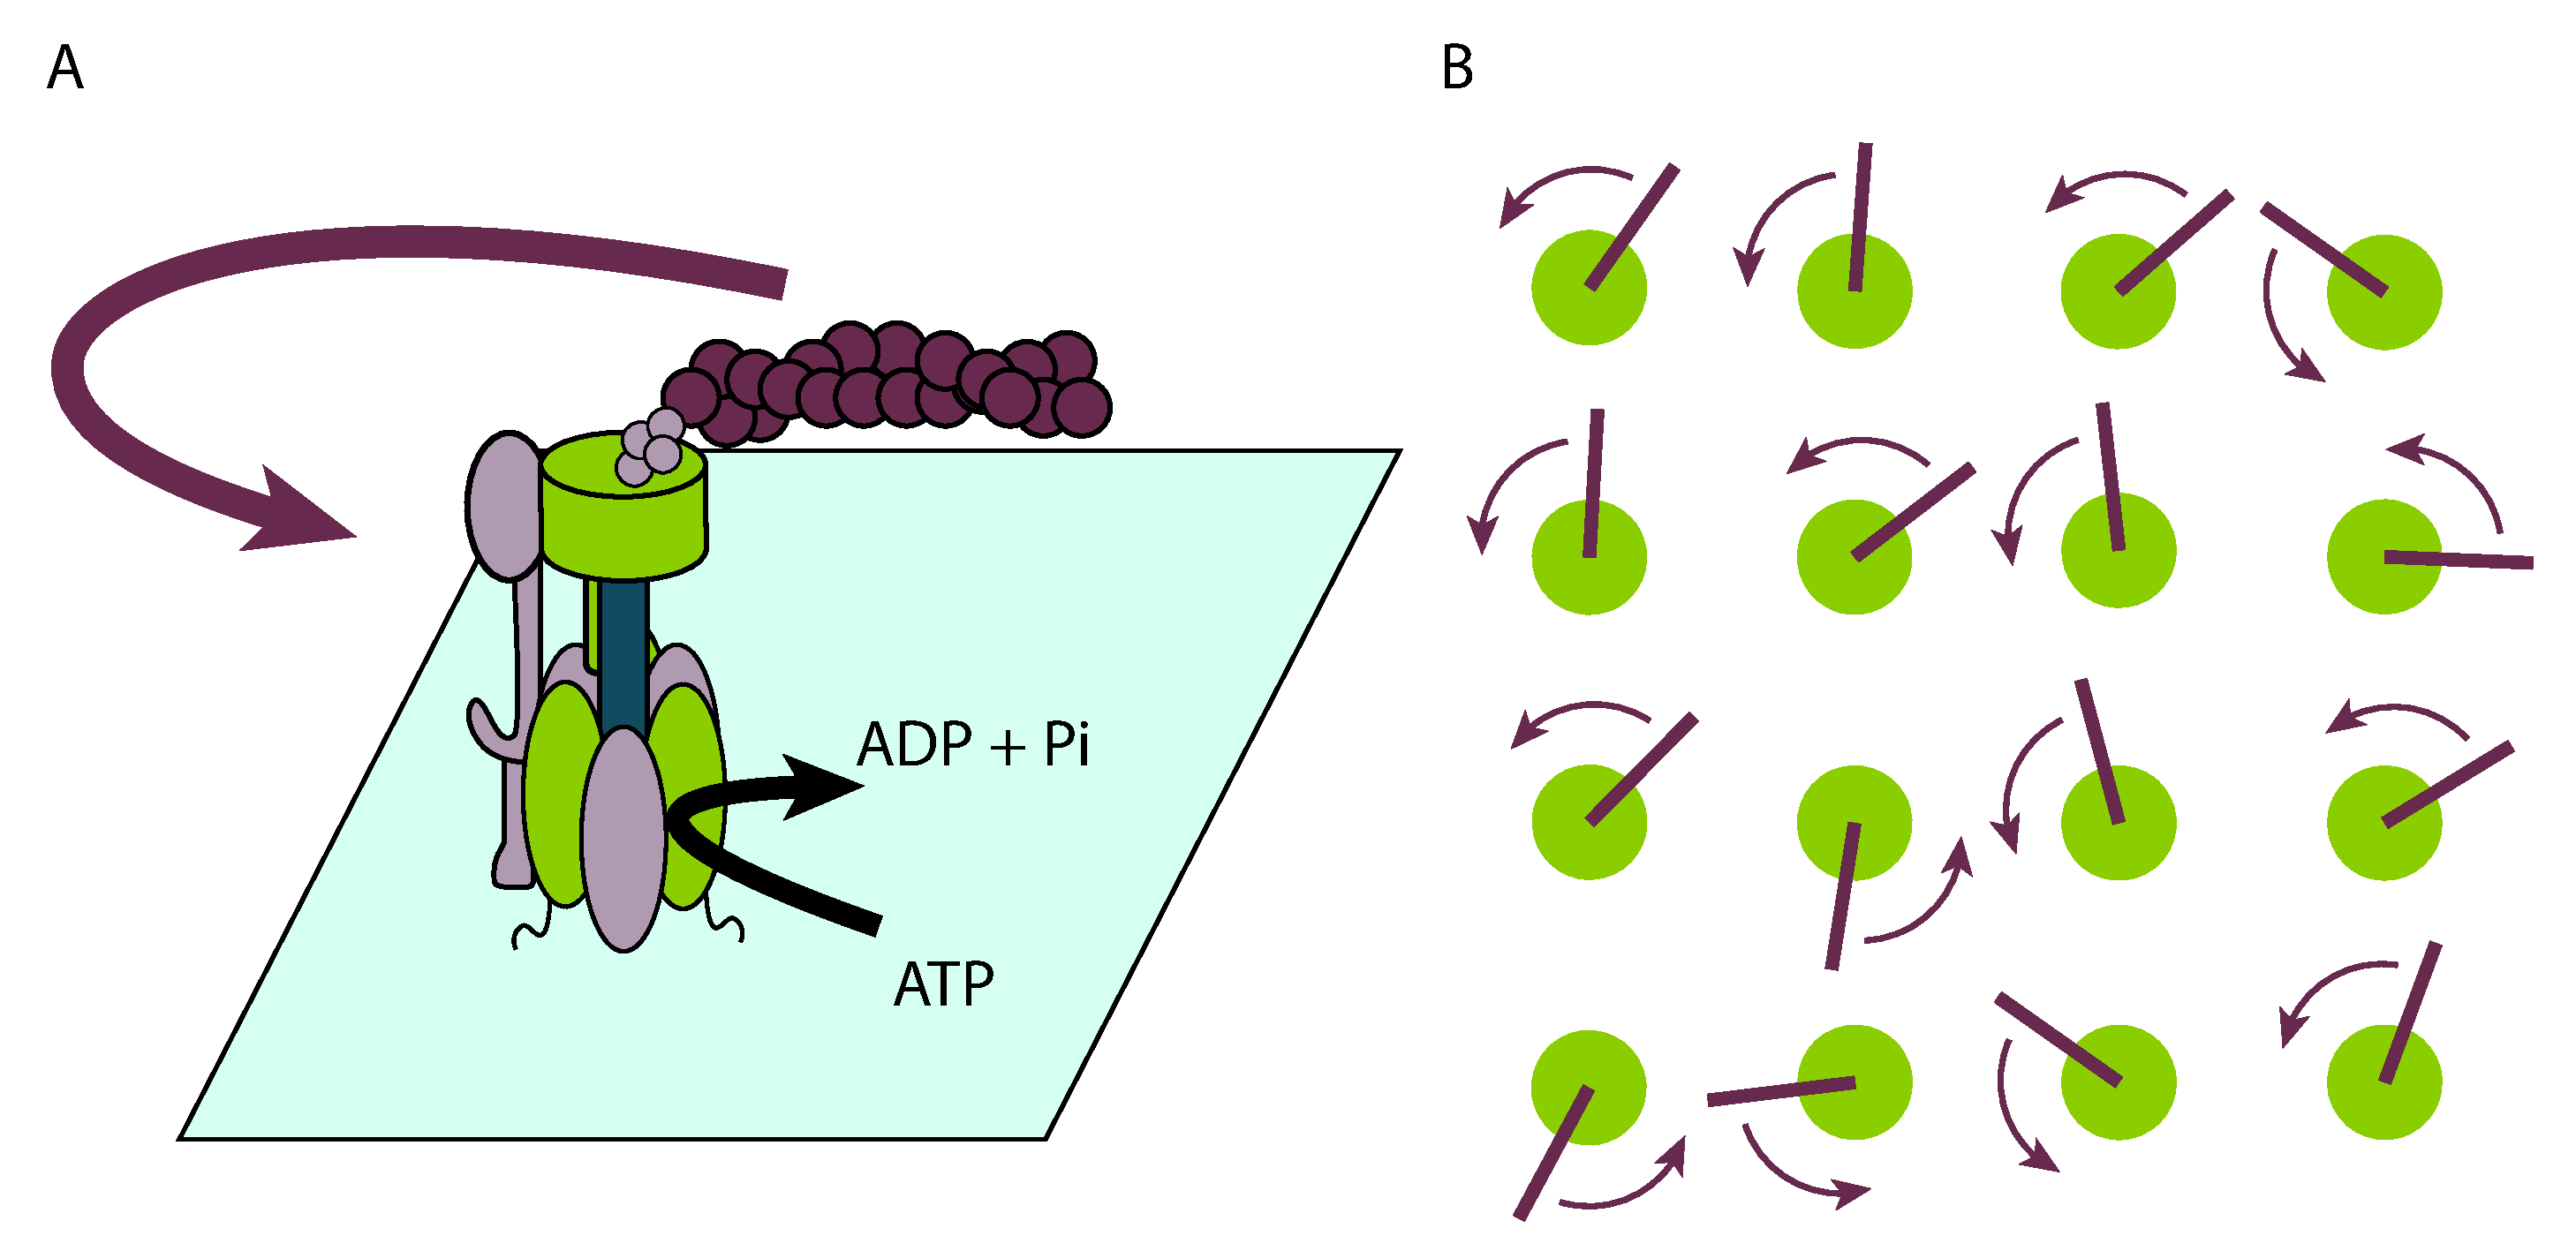
\includegraphics[width=1\linewidth]{figures/experimental_techniques_microscopy.pdf}
    \caption{\textbf{Experimental set-up to observe mechanical rotation of ATP synthase.} A) ATP synthase fixed to a surface and with an actin filament attached to its top sub-unit (F0 sub-unit, not labeled). When ATP is added to the environment, this enzyme hydrolyses it into ADP and a Phosphate group (Pi), which causes the top sub-unit to rotate (Image adapted from \cite{sambongi_mechanical_1999}). B) Top view (\gls{microscopy} perspective) of multiple labeled ATP synthase enzymes fixed to a surface and exposed to ATP. The actin filaments rotate as a result of ATP hydrolisation. This movement can be observed with \gls{microscopy} techniques.}
    \label{fig:chapter1:synthase_rotation}
\end{figure}


Similarly, techniques such as Förster Resonance Energy Transfer (FRET) or their single-molecule variant (smFRET) allow the measurement of proximity between molecules or two regions of the same molecule over a period of time. This technique works by attaching two fluorescent labels to the interacting regions or molecules (\figref{fig:chapter1:fret}). Each label has characteristic light excitation and emission wavelength (light colour) ranges (absorbs energy of light with colour X and emits colour Y), where the emission wavelength range of one bead overlaps with the excitation range for the second. When both beads are isolated and exposed to light in the excitation wavelength of the first label, the emission wavelength of the second label will not be observed. If these labels are in close proximity, \textcolor{red}{the energy obtained from exciting the first label is transferred to the second label via dipole-dipole coupling. Then, the latter will emit light in its emission wavelength, thus indicating proximity. This method's ability to measure molecular distances makes it suitable to study \glspl{ppi} and conformational changes \cite{truong_use_2001, heyduk_measuring_2002}.}
% the energy from the first label's emission will be absorbed by the second, which will emit light in its emission wavelength, thus indicating proximity. 
% This method can be employed, for instance, to identify protein conformational changes or \glspl{ppi} \cite{truong_use_2001, heyduk_measuring_2002}.
\textcolor{red}{The single molecule variant of FRET, smFRET, can be employed to measure protein dynamics by measuring fluctuations in FRET efficiency over time. These fluctuations are caused by changes in label spacing and is a direct measurement of protein conformational transitions \cite{weiss_measuring_2000}. These fluctuations reflect how often transitions occur that lead to changes in the spacing between labels.}

\begin{figure}[tbh!]
    \centering
    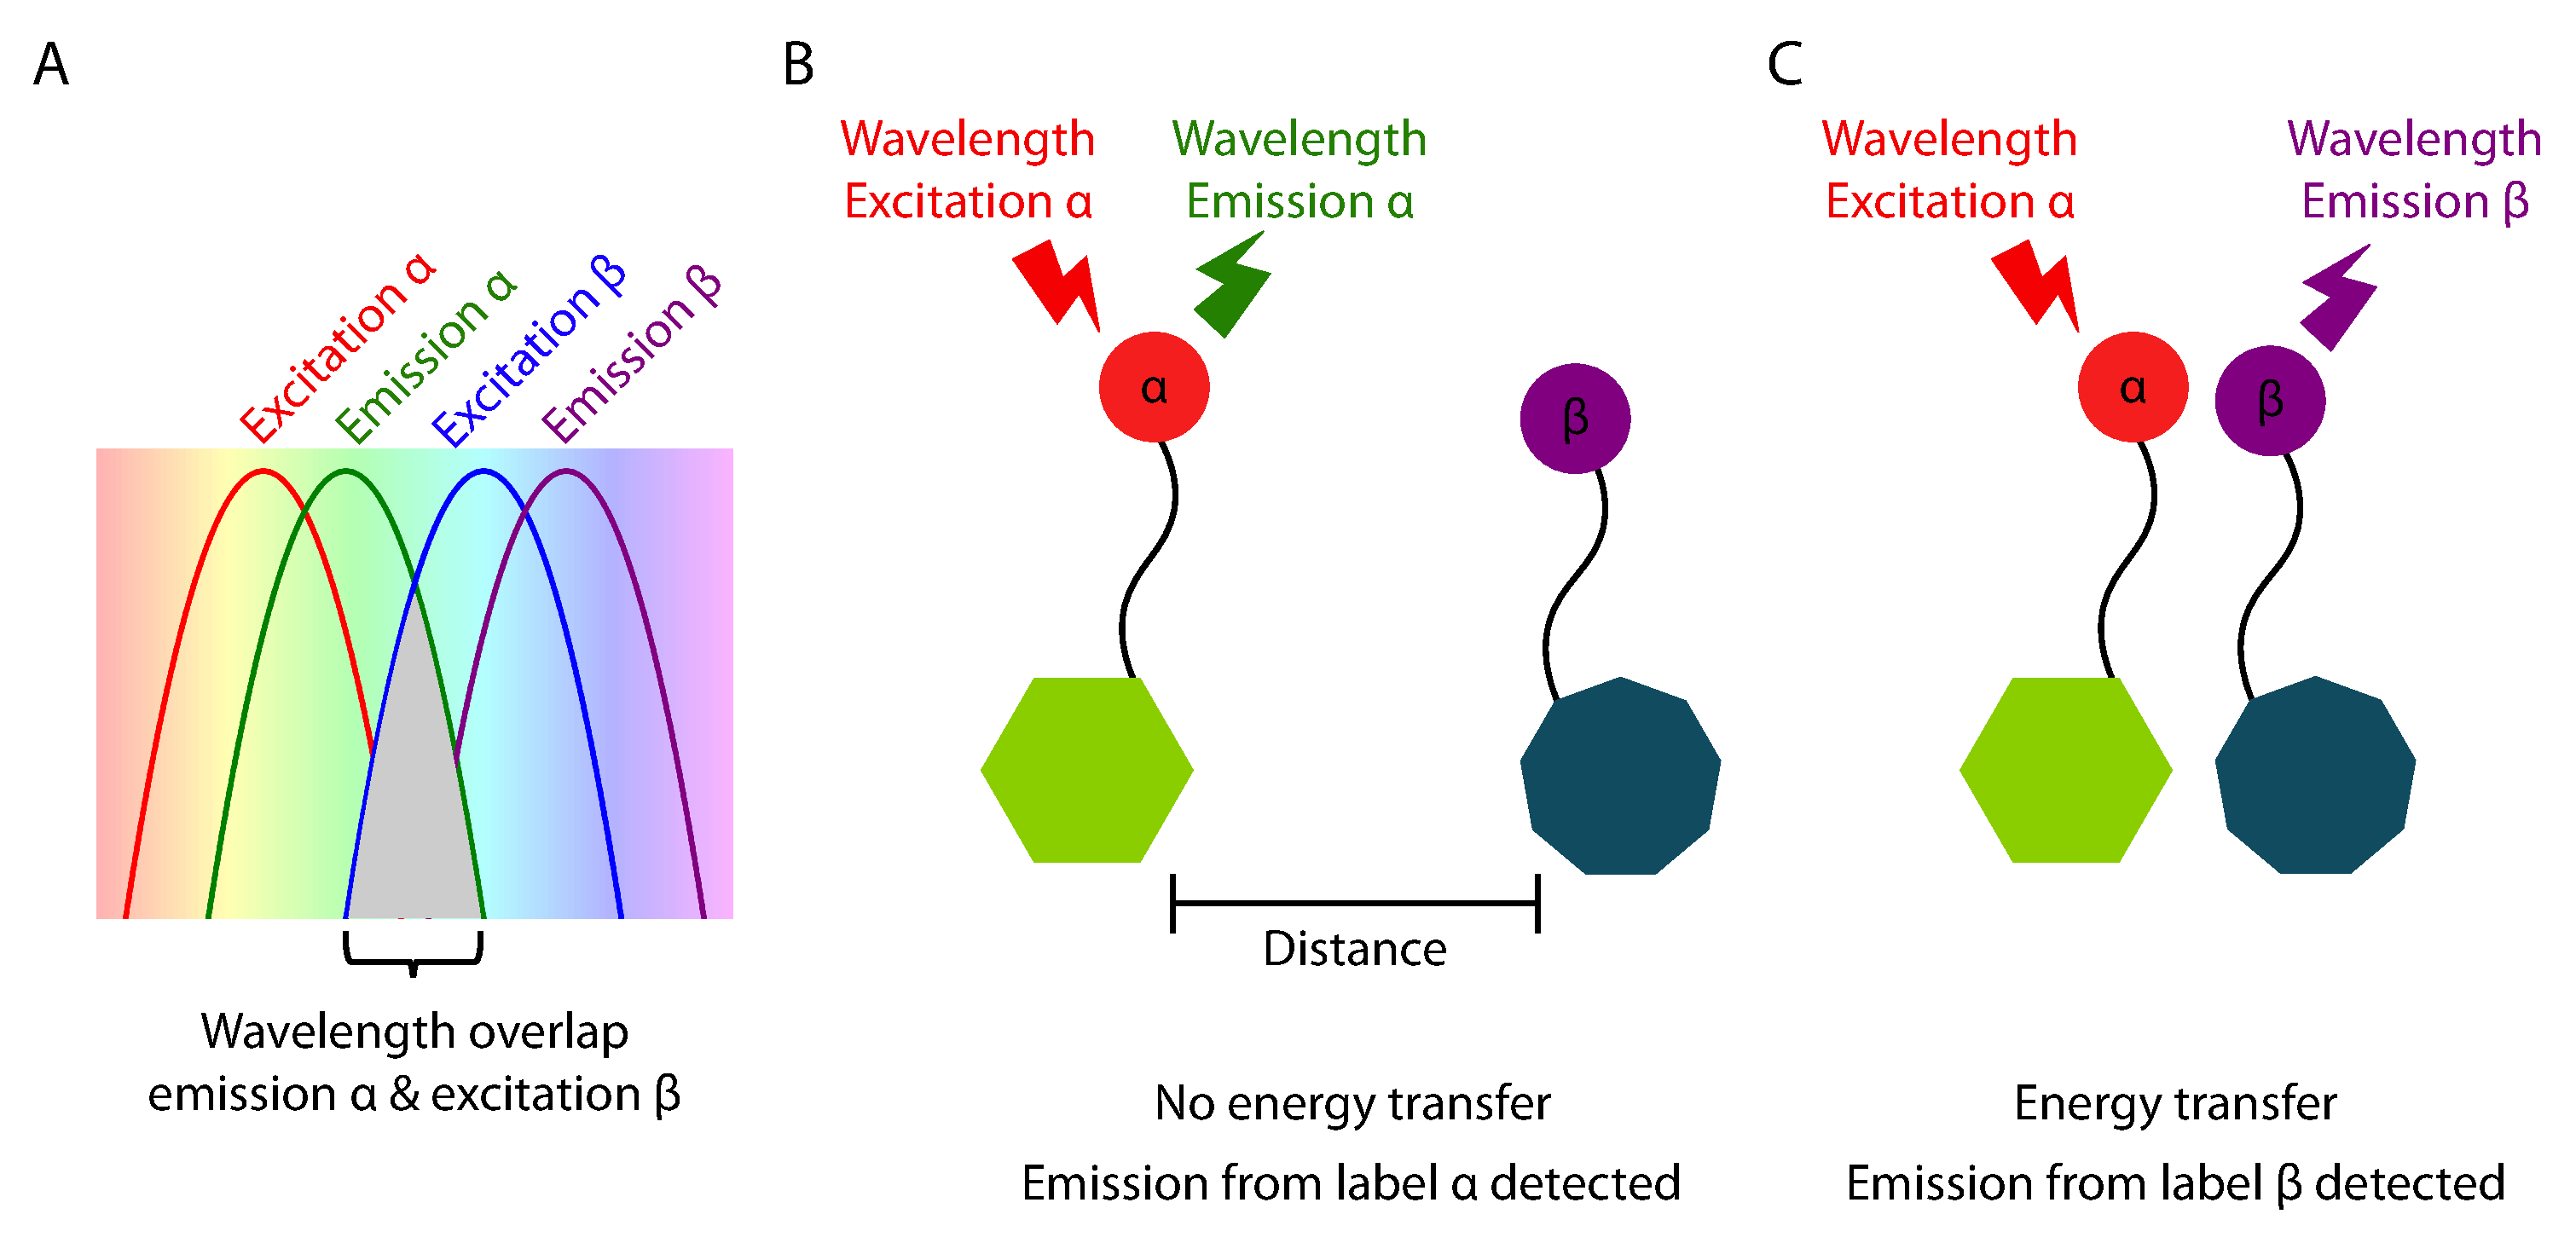
\includegraphics[width=1\linewidth]{figures/experimental_techniques_fret.pdf}
    \caption{\textbf{Förster Resonance Energy Transfer (FRET) mechanism.} A) The excitation and emission wavelengths of fluorescent dyes $\alpha$ and $\beta$. FRET is based on the energy transfer between two fluorescent dyes, in this example possible because dye $\alpha$'s emission wavelengths overlap with dye $\beta$ excitation wavelengths. B) Two distant proteins labelled with dyes $\alpha$ and $\beta$ and exposed to light with wavelength in the $\alpha$ excitation range. Energy cannot be transferred to dye $\beta$ and therefore dye $\alpha$ emits light. C) Two nearby proteins labelled with dyes $\alpha$ and $\beta$ and exposed to light with wavelength in the $\alpha$ excitation range. Energy is transferred from dyes $\alpha$ to $\beta$ and therefore dye $\beta$ emits light.}
    \label{fig:chapter1:fret}
\end{figure}

Other methods, such as Atomic Force \Gls{microscopy} (AFM), can be used not only to visualise molecules but also to study the folding and unfolding of proteins \cite{van_gils_protein_2024}. In addition to AFM's application in imaging, it can be used to pull from different regions of a protein and measure pulling forces, an application known as Single Molecule Force Spectroscopy (SMFS) \cite{hughes_physics_2016}. By attaching two protein regions to the AFM base and to the tip of its cantilever, the amino-acid chain can be pulled and relaxed to study its folding mechanics and \gls{dynamics} (\figref{fig:chapter1:afm}). Other techniques employ the same principle as AFM, but with different pulling strategies, namely Optical Tweezers \cite{bustamante_single-molecule_2020}, which pull with laser beams, or Magnetic Tweezers \cite{tapia-rojo_ephemeral_2019}, which pull with electro-magnetism.

\begin{figure}[tbh!]
    \centering
    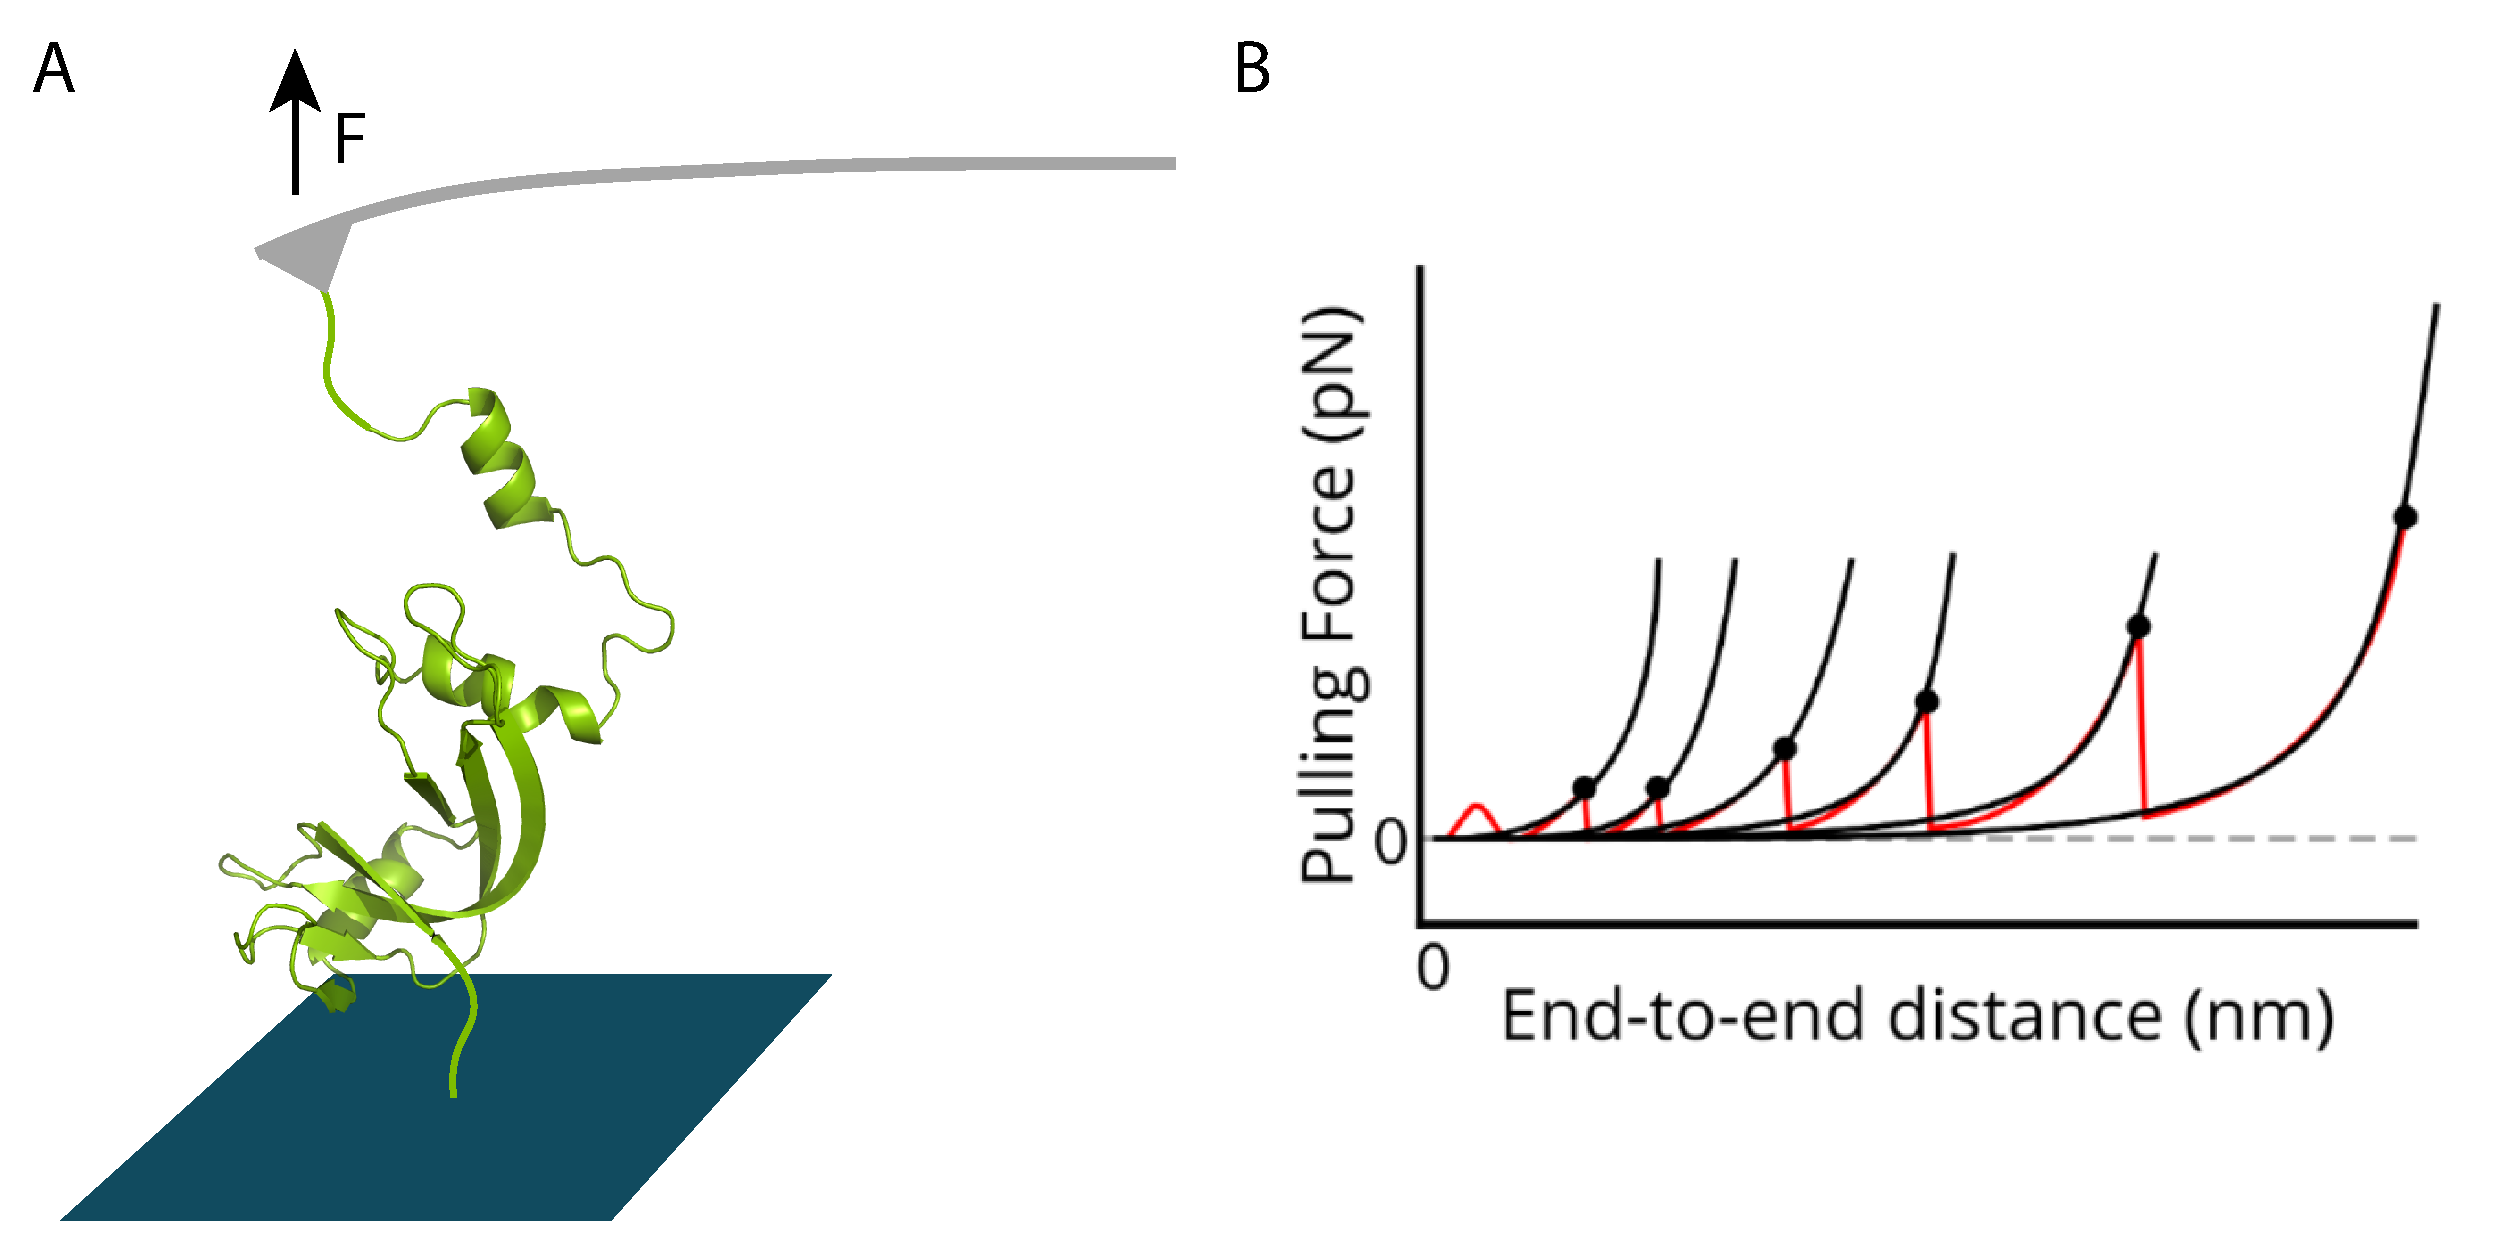
\includegraphics[width=1\linewidth]{figures/experimental_techniques_afm.pdf}
    \caption{\textbf{Atomic Force \Gls{microscopy} (AFM) pull-off force measurement.} A) A protein is attached to a base from one of its extremes and to the AFM cantilever from the other. The cantilever then pulls from the protein, gradually forcing it into a stretched \gls{conformation}. Pulling results on the sequential unfolding of the protein, which can be quantified by changes in pulling forces (PDB ID: 11BG \cite{vitagliano_potential_1999}). B) Force required to pull a protein to different extensions. Each peak indicates the loss of \gls{conformation} of a region (\textit{e.g.} a $\beta$-strand detached from a \gls{betasheet}). Subplot B extracted from \cite{van_gils_protein_2024}.}
    \label{fig:chapter1:afm}
\end{figure}


As much as these methods have been employed to elucidate the mechanisms and \gls{dynamics} of proteins, they rely either on labelling or on the binding of other external elements, which might interfere with the expected \textit{in vivo} \gls{dynamics}. 
Importantly, all the techniques discussed in this section are capable of measuring the behaviour of individual proteins, which might not be immediately obvious for some methods. For instance, whilst it is clear that AFM pull assays can monitor single molecules by stretching a single protein, other techniques (\textit{e.g.} FRET) can also be adapted to single-molecule studies. These techniques enable
the study of \gls{dynamics} across relatively large regions of a protein rather than at the per-residue level, which is central for understanding protein collective motions and conformational changes.


\subsection{Residue-Level Indirect Dynamic Measurements}

Several methods suited for protein structural determination have proven to be useful in the study of protein \gls{dynamics}. Here I will focus on \gls{xraycrystallography} crystallography and cryogenic electron \gls{microscopy} (\gls{cryoem}), both nowadays capable of producing structural models of proteins up to the atomic resolution \cite{yip_atomic-resolution_2020}. Although both \gls{xraycrystallography} and \gls{cryoem} can be used to model a single protein structure, their direct measurements reflect the conformations of multiple protein molecules rather than a single molecule. These techniques produce the vast majority of all available experimental \glspl{proteinstructure} \cite{noauthor_pdb_nodate_overal_statistics, noauthor_pdb_nodate_xray, noauthor_pdb_nodate_nmr, noauthor_pdb_nodate_cryoem}, which is also their most common application. These techniques occur under cryogenic and dehydrated conditions, far from \gls{physiologicalconditions}, to reduce protein motions as much as possible and thus increase resolution. Even under such non-native experimental conditions, there are strategies to study the dynamic properties of a protein from these structures. For instance, the conformational diversity of a protein with multiple defined \glspl{conformation} can be approximated simply by structurally aligning multiple static structures of the same protein \cite{monzon_codnas_2013, monzon_codnas_2016}. 


\gls{xraycrystallography} crystallography is a technique employed to obtain static \glspl{proteinstructure}. The sample preparation for this technique requires the crystallisation of the studied proteins. This process is non-trivial and often requires very dynamic protein regions to be trimmed to form the crystal or to prevent it from cracking due to large \gls{proteindomain} movements \cite{mooij_proteinccd_2009, gavrilov_nmr_2018}. Once the crystal is formed, an \gls{xraycrystallography} beam is passed through it, which will be diffracted by the protein's \glspl{electron}. The deflection pattern, which depends on the location of a protein's \glspl{electron}, is captured and modelled into a \gls{proteinstructure}. On individual \gls{xraycrystallography} structures, the low resolution or inability to model certain residues indicates that their atom's \gls{electron} cloud was too spread for assigning spatial coordinates \cite{smyth_x_2000}, thereby indicating considerable motion. For modelled residues, high \gls{electron} spread, hence low positional certainty and higher \gls{flexibility}, is represented with high residue \glspl{bfactor}---a metric of \gls{electron} density distribution in crystallography \cite{smyth_x_2000, carugo_b-factor_2022}; conversely, low \glspl{bfactor} indicate reduced \gls{electron} dispersion, higher positional certainty, and less \gls{flexibility}.


\Gls{cryoem} is a technique that does not require crystallisation, but it requires the protein samples to be rapidly cooled to reduce molecular motion and keep proteins near their native \gls{conformation} in a process named vitrification \cite{naydenova_reduction_2022, pfeil-gardiner_comparative_2019, bock_effects_2022, engstrom_high-resolution_2021}. These samples are then photographed in 2-dimensions with electron \gls{microscopy} (\glspl{electronmicroscopy}) from different angles, which will be computationally reconstructed into a 3-dimensional model of the protein. \Gls{cryoem} features equivalent metrics to \gls{xraycrystallography}'s \glspl{bfactor}, such as an \gls{aminoacid}'s local resolution \cite{yip_atomic-resolution_2020}, which also relates to the spread of a residue's \gls{electron} density. The interpretation of both these metrics carries an important consideration: though these metrics are based on quantifiable physical principles like \gls{electron} density and spread, they are still measured under conditions far from those in which the protein can be found \textit{in vivo} and therefore only proxy protein \gls{dynamics} under these non-\gls{physiologicalconditions}. It is not correct to extrapolate these measurements to \gls{physiologicalconditions}.

\subsection{Nuclear Magnetic Resonance Spectroscopy for Direct Dynamic Measurement}

A more adequate approach to studying protein \gls{dynamics} under near-\gls{physiologicalconditions} is the use of Nuclear Magnetic Resonance spectroscopy (\gls{nmr}), which allows in-solution measurements at physiological temperatures \cite{kleckner_introduction_2011, kuloglu_structural_2002}. \gls{nmr} applied to structure determination generates an ensemble of modelled structures, which serves as a sampling of a protein's conformationally allowed space.

Briefly, \gls{nmr} can identify the environment of an atom of interest with a 1/2 \gls{nuclearspin} \gls{nucleus} (atoms with specific configurations of \glspl{proton} and \glspl{neutron}), which makes the atom have a non-zero nuclear \gls{nuclearspin} (\figref{fig:chapter1:atom}). This confers the atoms magnetic properties, which can interact with a \gls{magneticfield} (\textit{e.g.} $^{1}\text{H}$ or simply ``\gls{proton}'', or $^{13}\text{C}$). These atoms are analysed based on the following basic principle: First, a strong \gls{magneticfield} is applied to a protein (or any other molecule), thereby aligning the \gls{nuclearspin} of its \gls{nucleus} with the direction of the \gls{magneticfield} \cite{marion_introduction_2013}. Then, an orthogonal \glspl{radiofrequency} (\gls{radiofrequency}) is pulsed, which temporarily shifts the orientation of the \glspl{nucleus}'s \gls{nuclearspin}. The \gls{electron} cloud of each atom and its neighbouring atoms determines the local magnetic environment and thus offers the \gls{nucleus} a different degree of shielding \cite{marion_introduction_2013}, which results in larger or smaller \gls{nuclearspin} transition and hence larger or smaller \glspl{chemicalshift}. As the \gls{nucleus}' \gls{nuclearspin} re-aligns with the original \gls{magneticfield}, changes in the \gls{magneticfield} at specific frequencies are detected by a coil surrounding the sample. These changes induce an electrical signal in the coil, which provides information about the \gls{nucleus}' degree of shielding when the \gls{radiofrequency} was applied. These frequencies are measured at once for all atoms of interest for each molecule in the sample, and then Fourier-transformed into spectra. The peaks in the spectra are then compared with the frequency of a reference standard, and measured in \glspl{ppm} (ppm). 
Given the size, connectivity and complexity of proteins, additional experiments are needed to resolve their structures, leading to the development of multi-dimensional \gls{nmr} methods. Some of these methods include \gls{cosy} (Correlated Spectroscopy), \gls{noesy} (Nuclear Overhauser Effect Spectroscopy) and \gls{hsqc} (Heteronuclear Single Quantum Coherence)  \cite{kline_determination_1988, kwan_macromolecular_2011}.

% \textcolor{red}{The NMR structural ensembles offer a range of conformations in which the protein can exist rather than structures of single molecules. In other words, every single model in the structural ensemble is derived from a population of molecules rather than capturing individual behaviours. In order to interpret the conformational space of a protein, ensemble averaging [ref], can be applied. This technique averages the coordinates of selected atoms (often those forming the protein backbone) to obtain an averaged or consensus structure. The spread of atomic coordinates can be calculated to obtain a measure of flexibility. This method allows a purely coordinate-based numerical representation of protein conformation and flexibility from NMR ensembles.}

\textcolor{red}{The NMR structural ensembles represent a range of conformations in which the protein can exist, reflecting the diverse structural states sampled by a population of molecules rather than individual static structures. Each model within the ensemble thus captures the collective behaviour of the molecular population, encompassing multiple conformations. Since NMR data yield an ensemble-averaged view of structural parameters---such as bond distances, angles, and dihedral angles---this averaging represents a comprehensive depiction of the protein’s conformational landscape rather than any single static structure. Averaging the NMR parameters across part of or the entire ensemble, NMR can provide insights into multiple conformations that might be present, as well as regions of stability and flexibility, as the ensemble reflects both the most probable structural features and the extent of their variation. In this way, ensemble-averaged parameters enable a probabilistic understanding of the protein’s structural landscape, suggesting areas of rigidity where parameter variation is low and regions of flexibility where it is high \cite{sutcliffe_representing_1993, stockelmaier_conformational_2024}. Although the ensemble does not capture dynamic transitions or timescales, it provides a statistical summary of the conformational possibilities that indicate the likely dynamic properties of the protein.}

% By analysing these conformational averages, we gain a deeper understanding of the protein’s potential functional motions, as each conformation represents not only a possible structure but also the likelihood of transitions between states, offering a window into the dynamic properties that may underpin its biological function.}

% \textcolor{red}{The NMR structural ensembles represent a range of conformations in which the protein can exist, reflecting the diverse structural states sampled by a population of molecules rather than individual static structures. Each model within the ensemble thus captures the collective behaviour of the molecular population, encompassing multiple conformations. As the data obtained from NMR represent averages, an interpretation of these ensembles is their own average...

% Ensemble averaging can be applied to obtain a representative conformation of 

% interpret this conformational space quantitatively, ensemble averaging \cite{sutcliffe_representing_1993} can be applied. }

% This technique involves averaging the coordinates of selected atoms, often those in the protein backbone, to derive an averaged or consensus structure. Additionally, calculating the spread of atomic coordinates provides a measure of flexibility for each region. Through this approach, ensemble averaging allows a coordinate-based, numerical representation of protein conformation and flexibility, directly derived from NMR ensembles.}


\begin{figure}[tbh!]
    \centering
    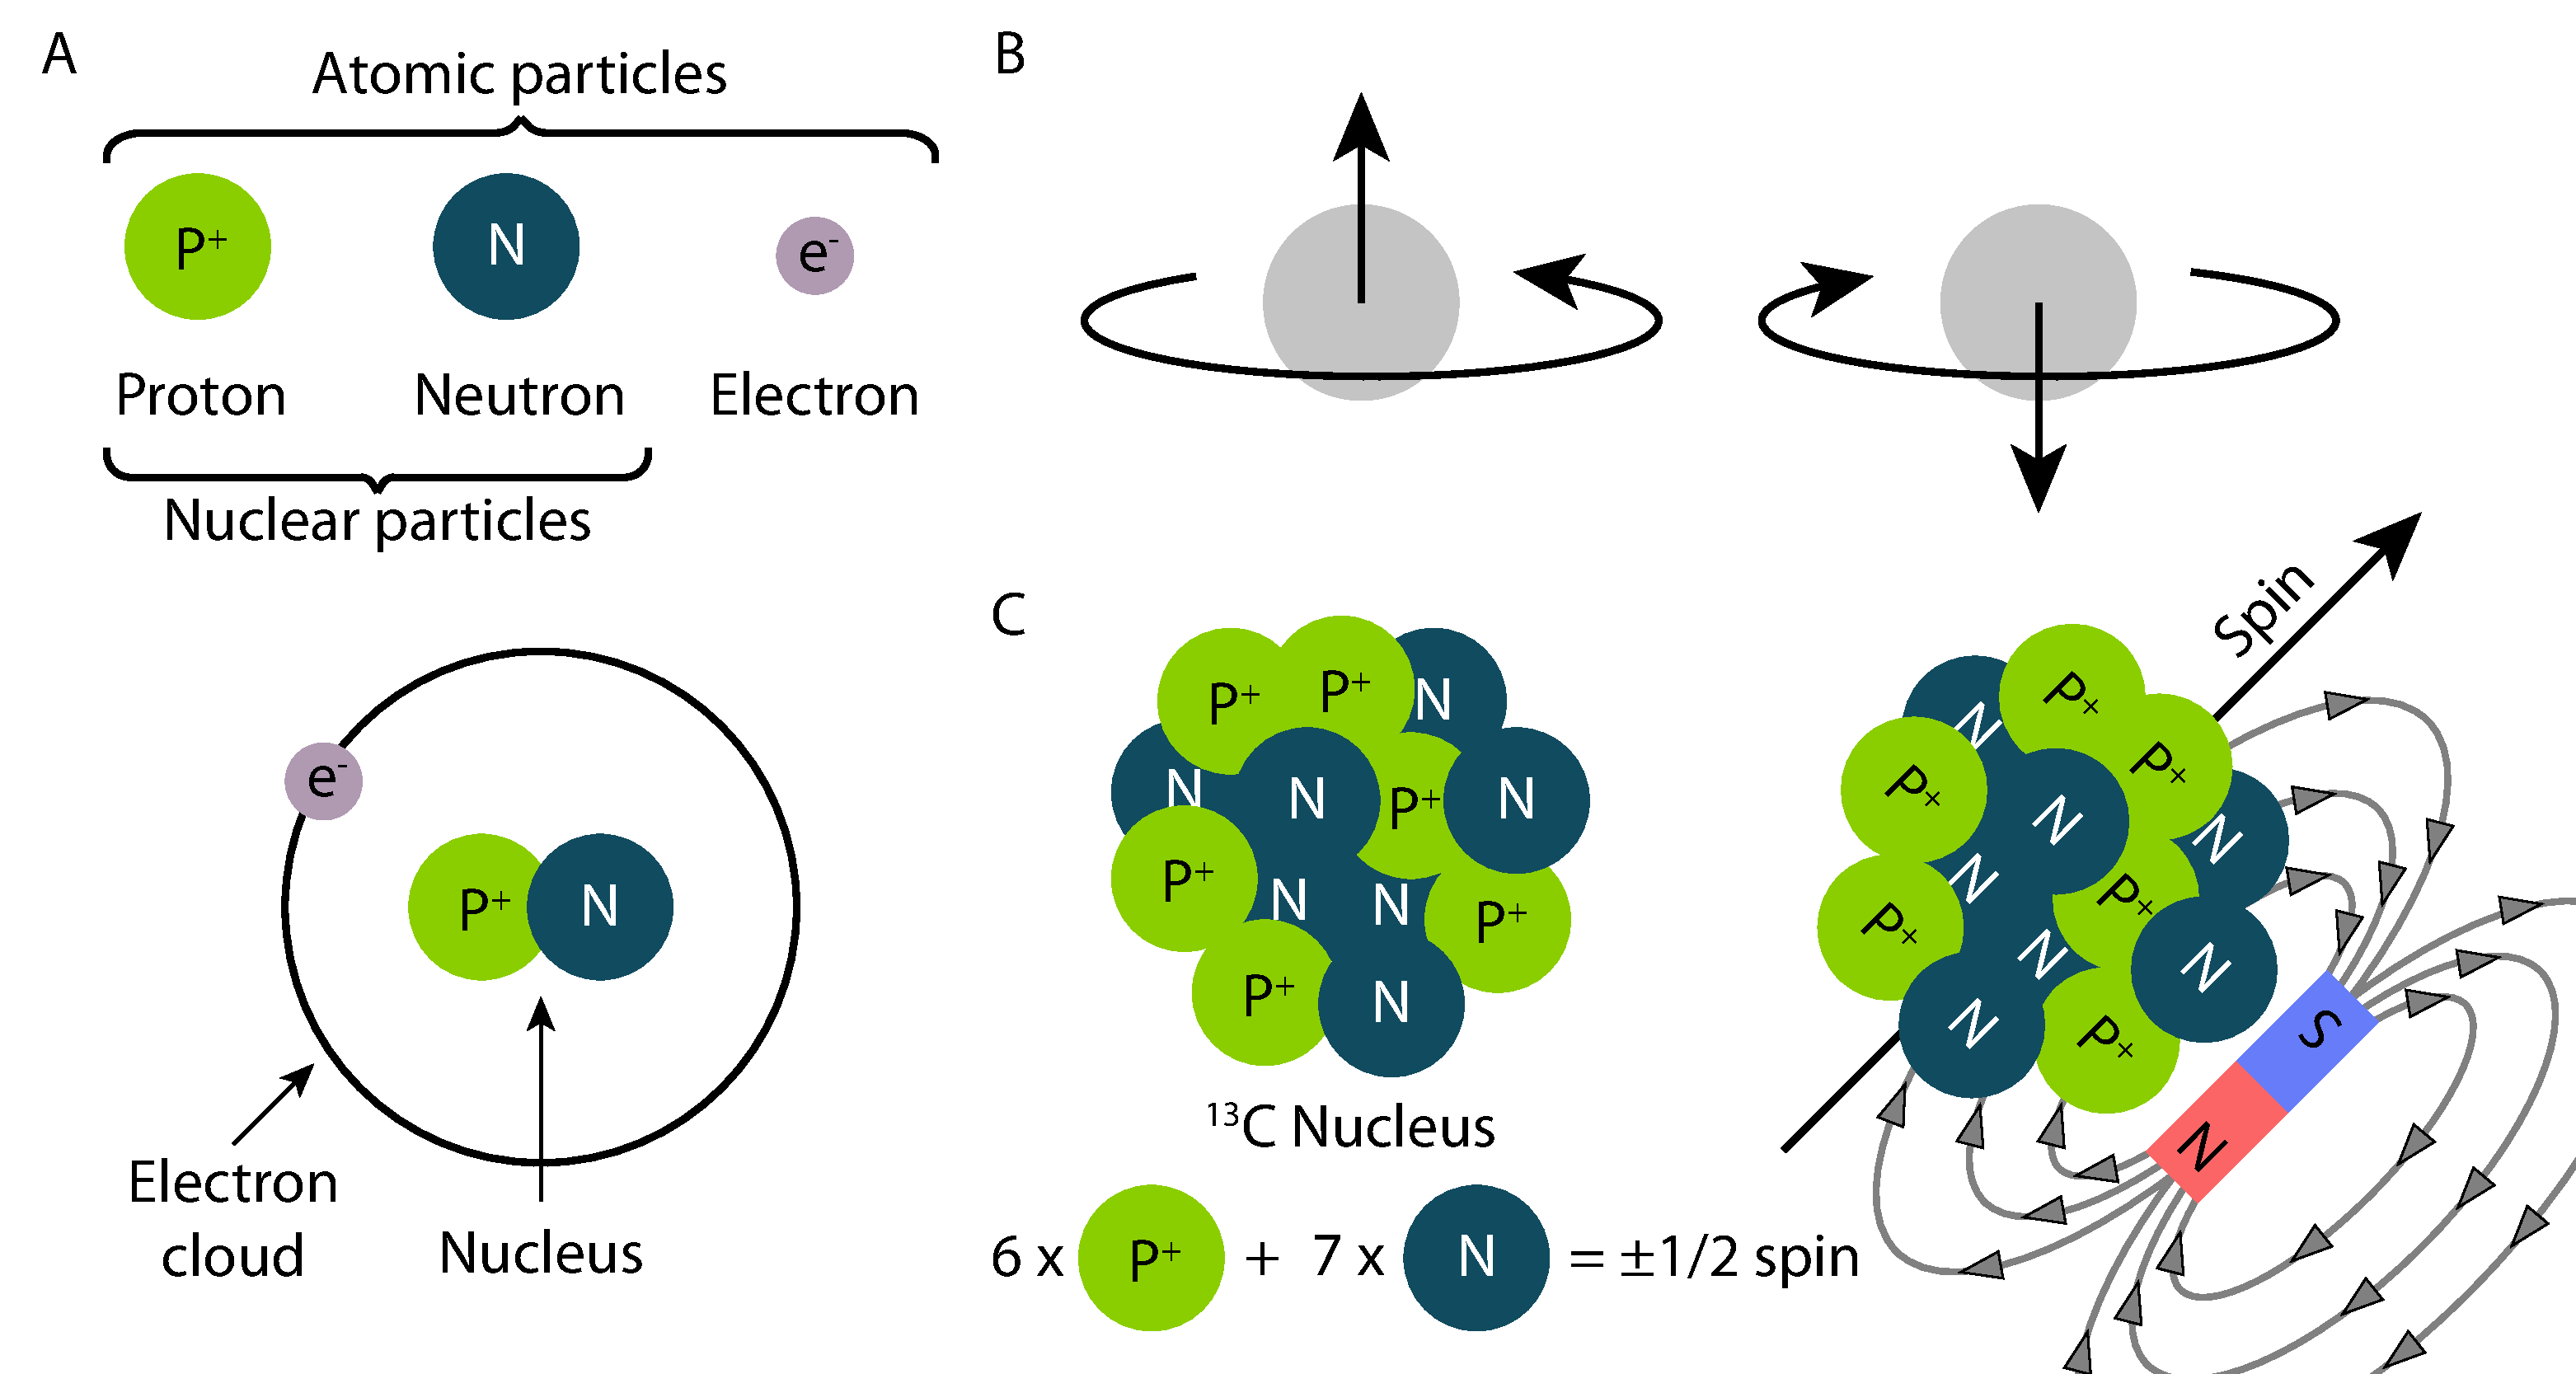
\includegraphics[width=1\linewidth]{figures/spin_nucleous.pdf}
    \caption{\textbf{Atom components and nuclear \gls{nuclearspin}.} A) An atom is composed of a combination of \glspl{proton}, \glspl{neutron} and \glspl{electron}, named atomic particles. \Glspl{proton} and \glspl{neutron} are located in the \gls{nucleus} of an atom and thereby constituting a subset of atomic particles: the nuclear particles. The \glspl{electron} exist in a cloud surrounding the \gls{nucleus}. B) Each atomic particle has an intrinsic angular momentum or \gls{nuclearspin}, which can be, in the case of atomic particles, projected as either ``up'' or ``down'' (different spins are allowed for other particles, but atomic particles feature only these two). This angular momentum is also called \gls{nuclearspin} because the behaviour of the particle is analogous to a sphere rotating with either right-hand or left-hand spinning, although the particles do not actually physically \gls{nuclearspin}. Atomic particles, specifically \glspl{proton}, \glspl{neutron}, and \glspl{electron}, are fermions (particles with half-integer \gls{nuclearspin}) with a \gls{nuclearspin} of 1/2. The allowed \gls{nuclearspin} projections for these particles are +1/2 and -1/2. C) The \gls{nucleus} of $^{13}\text{C}$ contains 6 \glspl{proton} and 7 \glspl{neutron}, which cannot balance each other out and therefore, the total nuclear \gls{nuclearspin} is ±1/2. This confers magnetic properties to the \gls{nucleus}, which can thereby be induced into an orientation by a \gls{magneticfield}. In this example, the \gls{nucleus} has a +1/2 \gls{nuclearspin} projection, and is thereby oriented in the same direction as the \gls{magneticfield}. 
    }
    \label{fig:chapter1:atom}
\end{figure}

\begin{figure}[tbh!]
    \centering
    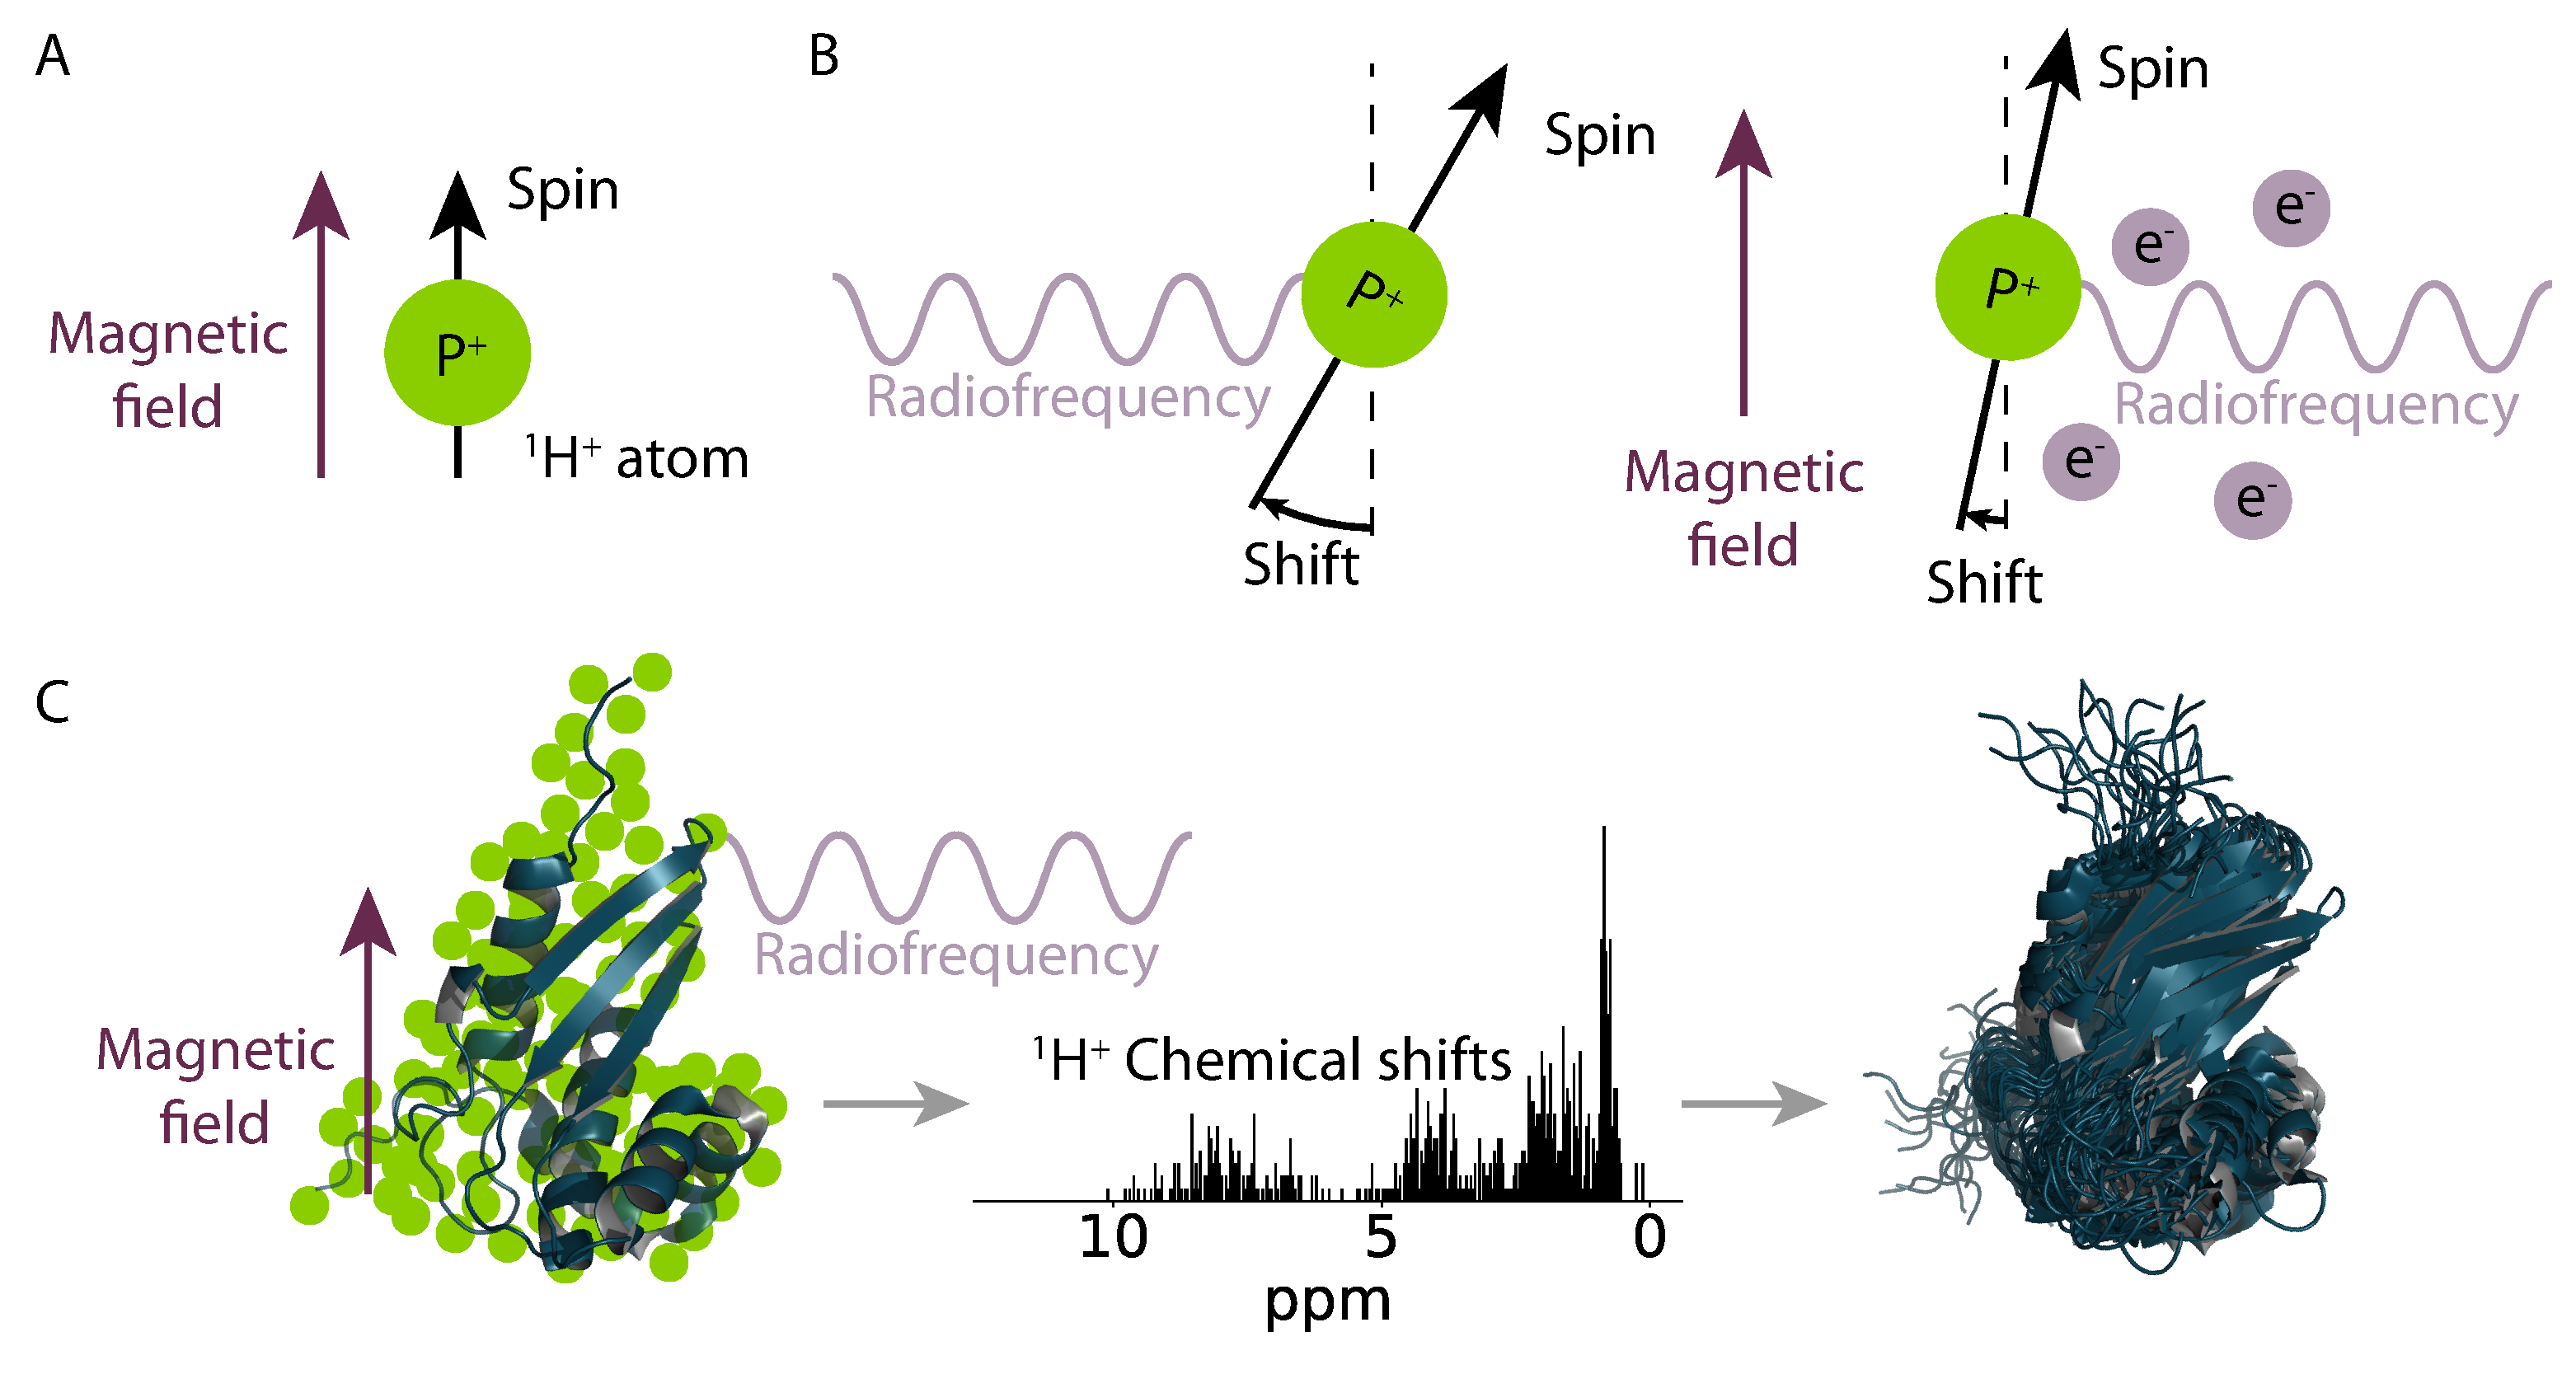
\includegraphics[width=1\linewidth]{figures/nmr_guts.pdf}
    \caption{\textbf{\gls{nmr} fundamentals illustrated with \gls{proton} \gls{nmr}.} A) The \gls{proton} in this example has a +1/2 \gls{nuclearspin} projection, therefore aligning to the \gls{magneticfield} generated by the \gls{nmr} machine (machine omitted in figure). B) The \gls{proton} is disturbed by a radiofrequency (\gls{radiofrequency}), perpendicular to the \gls{magneticfield}, which shifts the orientation of the \gls{proton}'s \gls{nuclearspin}. The \gls{proton} can be shielded in different degrees from the \gls{radiofrequency}, resulting in smaller shifts than an unshielded \gls{proton}. C) At the protein level, there are multitude of \gls{proton} atoms, each with different degree of \gls{electron} shielding, depending on their molecular context (their location in the protein). When the protein is perturbed with a \gls{radiofrequency}, \glspl{proton} shift their \gls{nuclearspin} alignment from the \gls{magneticfield}. While the \glspl{nucleus} \gls{nuclearspin} re-align with the \gls{magneticfield}, they induce electrical signals in the \gls{nmr} machine's detection coil, which captures their frequencies. These frequencies can be used to model the \gls{proteinstructure} as an ensemble of models, each representing an allowed \gls{conformation} for such protein. The \glspl{proteinstructure} in this figure  are models in the ensemble PDB ID 2M5H \cite{ouyang_solution_2013}.}
    \label{fig:chapter1:nmr}
\end{figure}


Beyond structure determination, \gls{nmr} can also be applied to the study of protein motions at the residue level. Two \gls{nmr} metrics are prominent in the study of protein motions: Random Coil Index (\gls{rci}) and $\text{S}^{2}$ order parameter (\gls{s2orderparameter}). \gls{rci} is a metric derived from comparing the \gls{chemicalshift} of an \gls{aminoacid}'s \glspl{nucleus} versus the expected unstructured \gls{chemicalshift} of such \gls{aminoacid} \cite{schwarzinger_random_2000}. This metric, therefore, offers a description of an \gls{aminoacid}'s \gls{flexibility} at slow time scales (micro- to milli-seconds), where near-zero values represent unstructured regions which can easily change \gls{conformation}, such as coil or turn, and higher values represent structured, more rigid \glspl{conformation}, such as \gls{alphahelix} or \gls{betasheet}. \gls{s2orderparameter}, on the other hand, offers a direct measurement of protein \gls{dynamics} at short time scales (pico- to nano-seconds) \cite{sapienza_using_2010}. It does so by measuring the amplitude of motion of the N-H (for \gls{backbone} dynamics) or C-H (for \gls{sidechain} dynamics) vectors relative to the protein \gls{backbone} after \gls{radiofrequency} perturbation \cite{sapienza_using_2010, smith_use_2021}. Together, they offer an overview of protein \gls{dynamics} and conformational tendencies at different time scales.


Some other variants of \gls{nmr} facilitate the study of diverse aspects of protein \gls{dynamics}, folding, and binding \cite{kleckner_introduction_2011}. Examples of these variants are real-time (RT) \gls{nmr} and residual dipolar coupling (RDC). 
RT-\gls{nmr} provides information about the structural evolution of proteins subject to a certain environment. It does so by measuring \gls{nmr} spectra over time after the introduction of a new condition (\textit{e.g.} the addition of a binder). Over time, the intensity from the frequencies in the starting \glspl{conformation} diminish as the ones from the final \glspl{conformation} increase \cite{zeeb_protein_2004}. 
RDC arises when molecules experience partial alignment in a \gls{magneticfield}, leading to detectable dipolar interactions between nuclear spins. RDCs offer angular constraints that reveal relative orientations and distances of protein domains, providing insights into the global fold and conformational changes of proteins \cite{tolman_nmr_2006}. This technique requires special alignment media to induce partial alignment, unlike RT-\gls{nmr}, which can be measured under standard \gls{nmr} conditions. RDCs are particularly useful for studying large proteins and complexes, complementing traditional \gls{nmr} techniques by providing long-range structural information \cite{tolman_novel_2002, bax_weak_2003}.

This brief introduction to \gls{nmr} focuses on protein structural diversity, \gls{flexibility}, and \gls{dynamics}, but this technique's polyvalence enables applications such as the study of folding mechanisms \cite{peacock_hydrogendeuterium_2021}, the observation of conformational changes at different temperature and pH ranges \cite{gerken_measurement_2011}, and binding mechanics \cite{dubey_role_2020}. Notable drawbacks of \gls{nmr} are the difficulties in studying large proteins \cite{frueh_nmr_2013} and the lower resolution of its elucidated structures compared to \gls{xraycrystallography} crystallography or \gls{cryoem} \cite{kwan_macromolecular_2011}. Arguably, the latter is not a drawback, but a feature created by the motion of proteins in near-\gls{physiologicalconditions}.

\subsection{\textcolor{red}{Complementary Spectroscopic Techniques}}

\textcolor{red}{In addition to NMR, other spectroscopic techniques, such as Electron Paramagnetic Resonance (EPR) and Circular Dichroism (CD), provide complementary insights into protein dynamics at the molecular level. EPR spectroscopy is used to investigate molecular interactions by measuring the magnetic properties of unpaired electrons (\textit{e.i.} electrons that solely occupy an orbital) introduced through site-specific spin labelling. This method enables precise measurement of distances in the nm range, making it suitable for detecting conformational changes and the motion of labelled sites within proteins \cite{sahu_electron_2020}.}

\textcolor{red}{CD spectroscopy, on the other hand, assesses secondary structural content by examining the differential absorption of left- and right-handed circularly polarised light. These two polarisation types interact differently with chiral molecules, like proteins, and are absorbed to varying degrees depending on the secondary structure. $\alpha$-helices, $\beta$-sheets, and random coils each have distinct CD spectra, as the unique chiral arrangements within these structures selectively absorb and rotate polarised light to differing extents \cite{greenfield_using_2006}. Changes protein conformation are directly related to variations in CD spectra. By capturing these variations, CD enables analysis of protein folding, stability, and structural transitions under various conditions.}

\section{Computational Study of Protein Motions}
\subsection{Molecular Dynamics}

Beyond the insights on protein conformational diversity and protein \gls{dynamics} that experimental methods can provide, diverse computational methods offer complementary information on a protein's dynamic nature. Notably, the use of Molecular Dynamics (\gls{md}) simulations is a flexible method that can be applied to problems such as drug-target binding \cite{de_vivo_role_2016}, effects of post-translational modifications \cite{sostaric_molecular_2021, bickel_effects_2024}, and the study of \glspl{idp} \cite{shrestha_full_2021}. 
In \gls{md} simulations, molecules are represented by a Newtonian physics model, where interactions are depicted as mechanical forces, such as Hooke's law \cite{adcock_molecular_2006}. Numerical integration over these forces allows the simulation of molecular motion over time, which generates time series of \glspl{conformation} or structures known as trajectories \cite{adcock_molecular_2006}.
\gls{md} simulations calculate the trajectories that a molecular system (\textit{e.g.} a protein monomer in solution) follows over a period of time (typically nano- to milli-seconds) \cite{lindorff-larsen_picosecond_2016}. 

These trajectories are calculated by first setting up the molecular system with initial coordinates and velocities, where velocities are the speeds and directions of atomic movement. The system's interactions are defined using a force field, a mathematical model that describes the potential energy of the system as a function of atomic positions. This includes terms for bonded interactions (bonds, angles, dihedrals) and non-bonded interactions (\gls{vandewaalsforces}, \gls{electrostaticinteractions}). After energy minimisation to remove steric clashes (unrealistically close contacts between atoms that cause high repulsive forces), the system is equilibrated to the desired temperature and pressure. Newton's equations of motion are then solved iteratively using numerical integration methods which consider atomic position, velocity, and acceleration (like the Verlet algorithm) to update atomic positions and velocities over time. These coordinates are saved at regular intervals, creating a time series of molecular \glspl{conformation} called trajectories. The sequential nature of these trajectories, the sampled structures in the \gls{md} simulation can be analysed as a timeline, possibly elucidating mechanisms that would be observed with difficulty from \gls{nmr} ensembles. 

Some metrics to extract information from \gls{md} simulations include Root Mean Square Deviation (\gls{rmsd}), Root Mean Square Fluctuations (\gls{rmsf}), and Circular Variance (\gls{cv}), which measure a protein's \gls{flexibility} both in the \gls{cartesianspace} or \gls{dihedralspace}. The \gls{rmsd} is a global metric of coordinate deviation from a reference structure, which can be used to simply identify large conformational changes through the trajectory. The \gls{rmsf} is a local per-residue (or atom) measure of deviation from a reference structure. Similarly to \gls{rmsd}, it can be used to detect changes in \glspl{conformation}, but it also identifies which residues are more affected by such changes. Both \gls{rmsd} and \gls{rmsf} are dependent on structural superposition to a reference structure, and thus sensitive to large structural shifts with a distant origin, such as those stemming from hinge regions. The \gls{cv} measures the changes in a residue's $\phi$ and $\psi$ angles over the course of an \gls{md} simulation. This makes the method superposition-independent, especially useful for proteins where a canonical reference structure is not available, such as IDPs or \glspl{idr}. Following the previous example, distant residues from the hinge region will not be deemed as highly motile, as with \gls{rmsf}, unless they experience dihedral changes themselves. In the context of this thesis, \gls{md} simulations were used to generate \gls{conformation} ensembles of a wide variety of proteins which were further analysed with Constava, a method developed as part of this work to quantify the allowed range of conformational states that proteins are capable of adopting and their capacity to transition among them (chapters \ref{chapter:contributions} and \ref{chapter:constava}).

\subsection{Normal Mode Analysis}

Another computational method to study protein motions is Normal Mode Analysis (\gls{nma}). This method calculates harmonic fluctuations around a \gls{proteinstructure}, in a computationally inexpensive manner, assuming that such structure represents the protein's \gls{globalminima} energy state \cite{wako_normal_2017}. While \gls{nma} can detect large-scale movements such as \gls{proteindomain} motions, it is limited by its harmonic and linear nature. \gls{md} simulations, on the other hand, are not restricted to linear motions and can more accurately describe complex conformational changes. Nevertheless, \gls{nma} is a powerful tool for rapidly probing a protein's \gls{flexibility} or to be applied to large-scale analysis due to its low computational requirements, as it was employed for the large-scale analysis of AlphaFold2 models in chapter \ref{chapter:plddt}.


\section{Protein Biophysics Computational Tools}

\subsection{Machine Learning in Biological Research}

Biological research has employed computational methods beyond the calculation of trajectories and harmonic movements. The development of data-centred models enables the quick extraction of information from a biological system, its analysis, and the definition of a set of labels or characteristics. These models perform their analysis in a structured manner, following a set of quantitative rules that determine the output of a system's analysis. This approach contrasts with human assessments, which are more prone to the introduction of qualitative criteria. The simplest family of models is the rule-based models, which are programmed to operate based on a predefined set of rules set by human experts (\textit{e.g.} a manually-created decision tree to determine from a \gls{proteinstructure} whether an \gls{aminoacid} is part of an \gls{alphahelix}). In contrast to this strategy are Machine Learning (\gls{machinelearning}) models, which learn the rules to perform a task from exposure to data. \gls{machinelearning} models require the definition of a model structure to be trained by exposing it to relevant data to learn how to perform a task (\figref{fig:chapter1:ml_basics}). \Glspl{supervisedlearning} \gls{machinelearning} models require the presence of labelled data for their training, which are employed for applications such as medical diagnosis \cite{kourou_machine_2015, capper_dna_2018}, personalised toxicity prediction \cite{vo_overview_2020, badwan_machine_2023}, and the estimation of protein properties \cite{cilia_protein_2013, orlando_accurate_2020, raimondi_exploring_2017, orlando_prediction_2022}. \Glspl{unsupervisedlearning} models are also widely used in biology to learn the structure of data \cite{chou_predicting_2006, maisuradze_principal_2009} or for feature extraction \cite{vaswani_attention_2023, church_word2vec_2017}. Complex model structures allow the combination of \gls{supervisedlearning} and \glspl{unsupervisedlearning} models. For the purpose of this work, we will focus on \glspl{supervisedlearning} models.


\begin{figure}[tbh!]
    \centering
    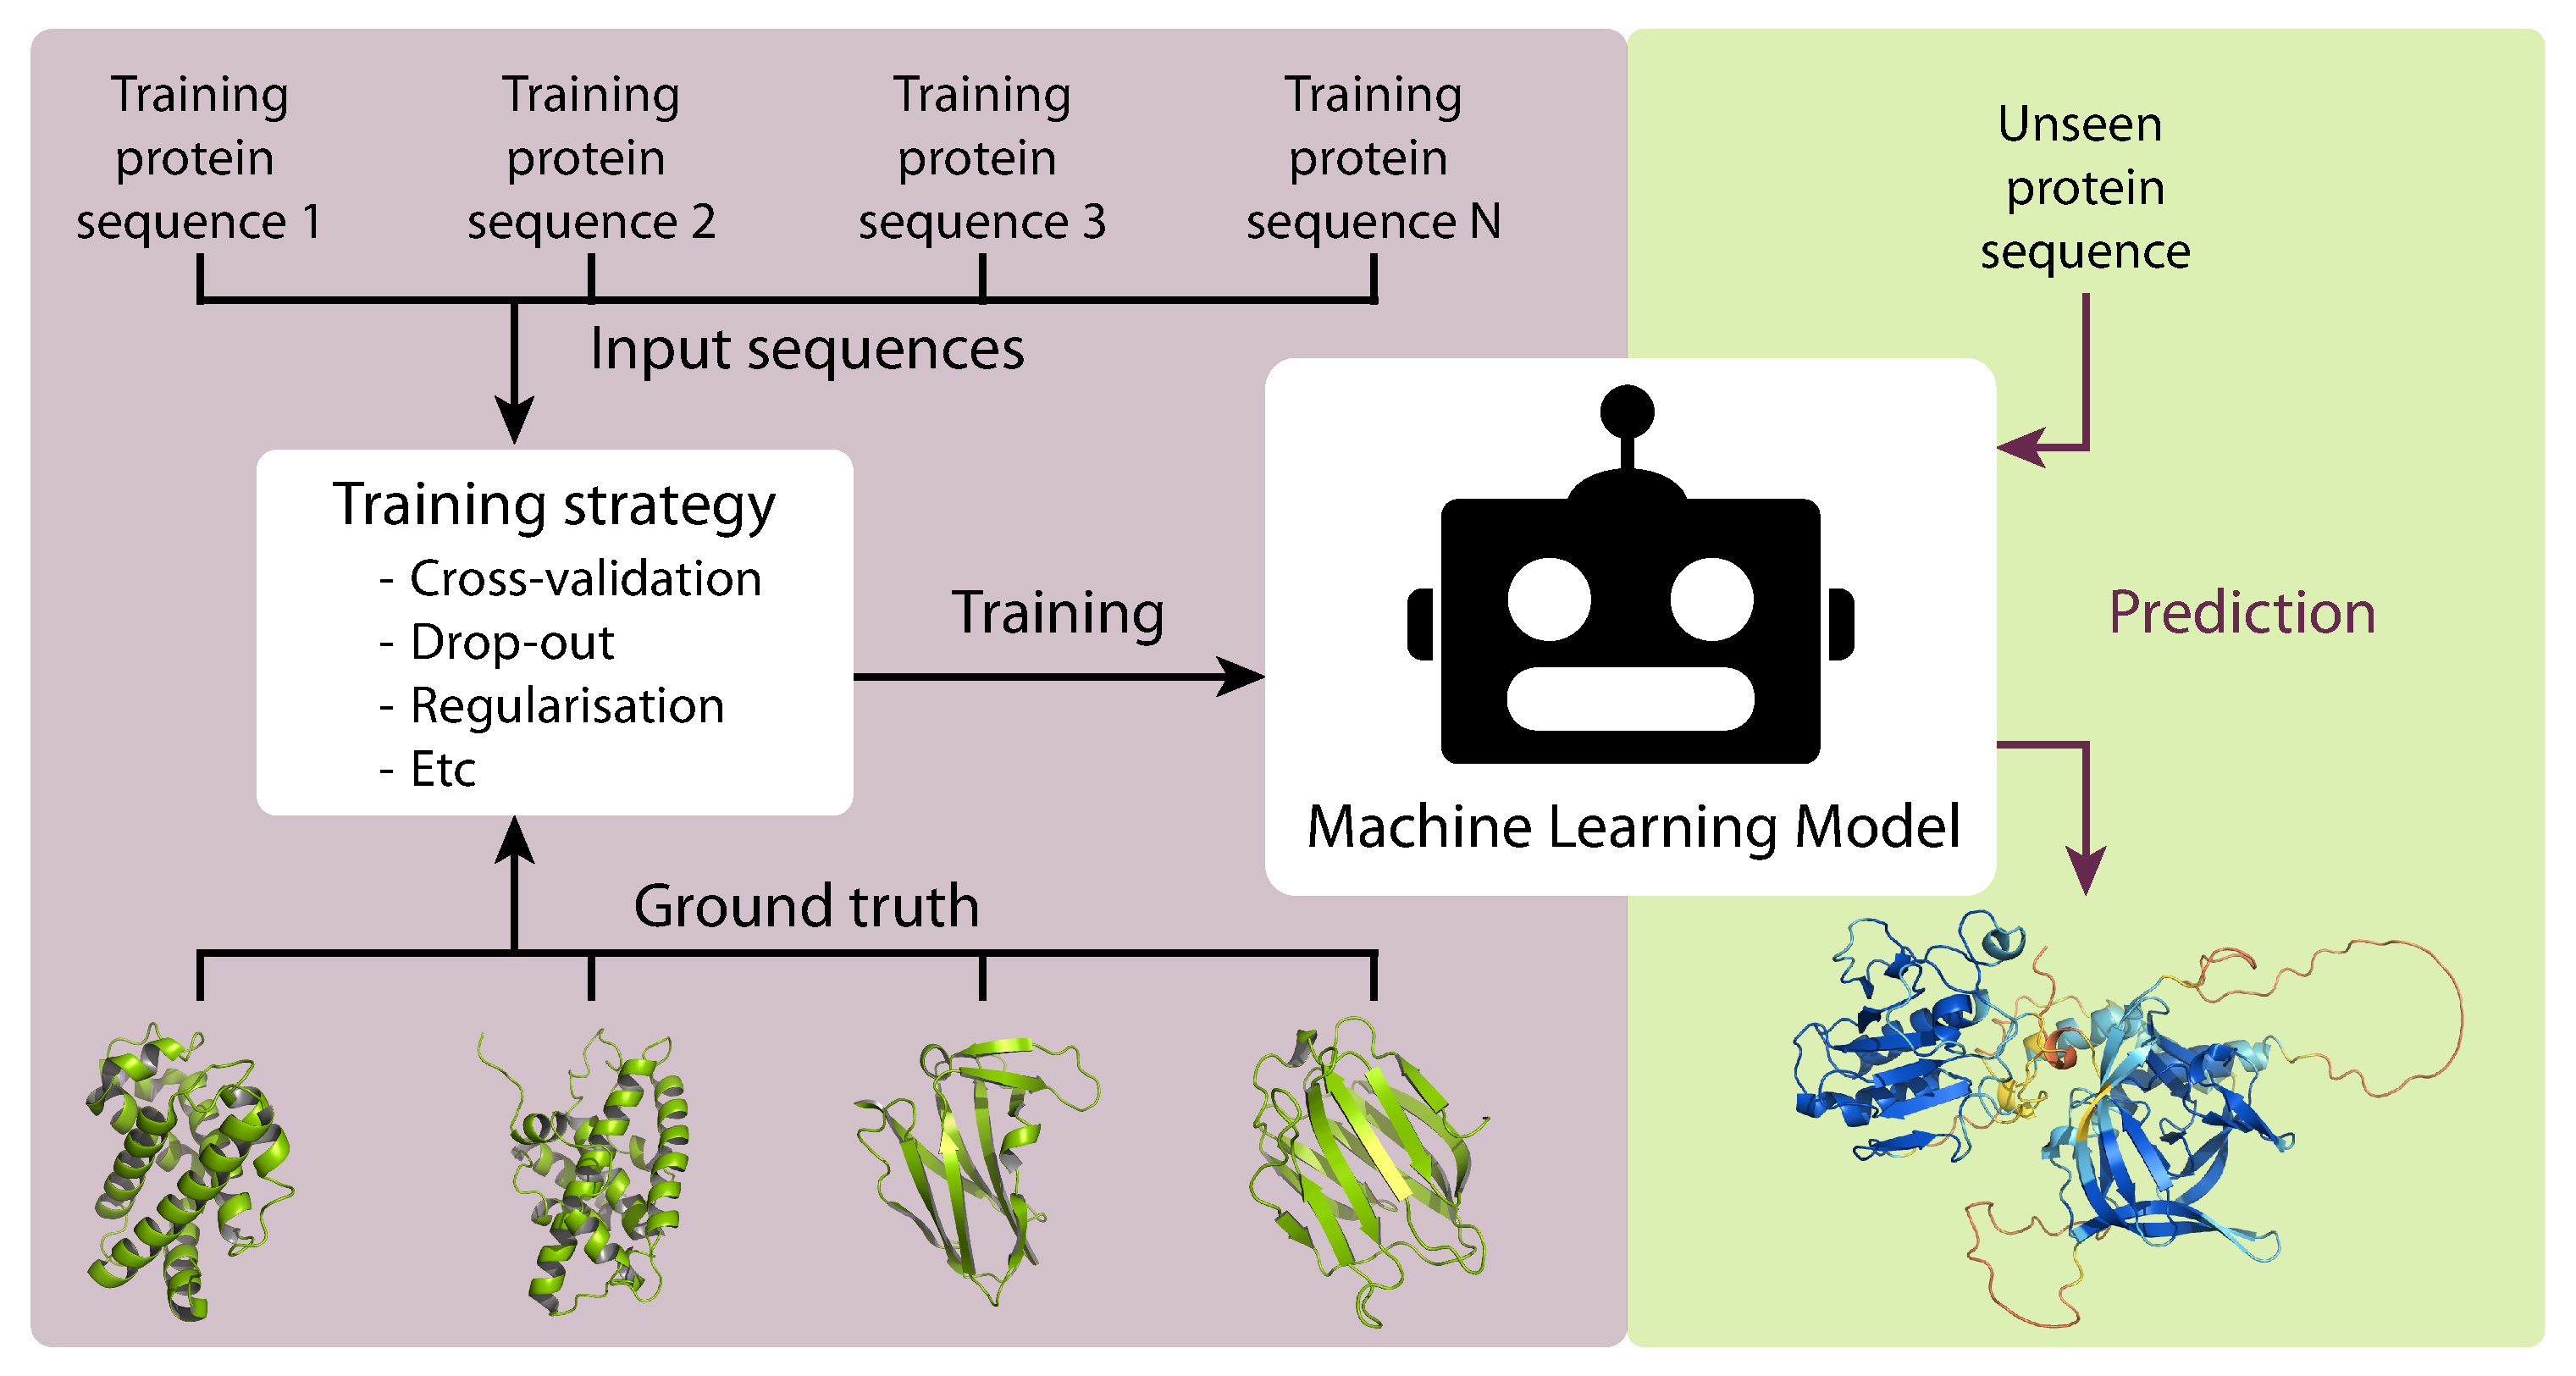
\includegraphics[width=0.95\linewidth]{figures/ml_basics.pdf}
    \caption{\textbf{Machine learning (\gls{machinelearning}) model basic training and prediction.} The general framework of a \glspl{supervisedlearning} \gls{machinelearning} model designed to predict \gls{proteinstructure} from its sequence uses as training data protein sequences and their corresponding \glspl{proteinstructure} as ground truths or expected outcomes. The training data is presented to the model according to the training strategy, which deploys methods to obtain a model able to correctly generalise (left). Strategies such as cross-validation prevent model ``overfitting'' (training data is learnt too well, capturing noise and details that do not generalise to new, unseen data, leading to poor performance on the latter). The trained model can then predict the structure of new, unseen protein sequences (right). \Glspl{proteinstructure} in the training diagram (left) with PDB IDs: 101M \cite{smith_robert_david_correlations_1999}, 1AD6 \cite{kim_structural_1997}, 1AKP \cite{constantine_sequential_1994}, and 1A3K \cite{seetharaman_x-ray_1998}. Predicted \gls{proteinstructure} (right) downloaded from \burl{https://alphafold.ebi.ac.uk/}, id Q15465.}
    \label{fig:chapter1:ml_basics}
\end{figure}


During the training process of \gls{supervisedlearning} models, the model adjusts its parameters, generally iteratively, to minimise the error between its predictions and the actual outcomes \cite{loog_chapter_2018}. The training process is assessed using metrics appropriate for the type of data. For discrete labels (\textit{e.g.} to classify whether a biological sample contains cancer), metrics such as \gls{accuracy}, \gls{precision}, \gls{recall}, and \Gls{f1score} \cite{naidu_review_2023} are used, while for continuous labels (\textit{e.g.} the prediction of a protein region's \gls{backbone} dynamics), metrics such as \Gls{meansquarederror}, \gls{rootmeansquarederror}, \gls{meanabsoluteerror}, and \gls{rsquared} \cite{botchkarev_performance_2019, chicco_coefficient_2021} provide insights into the model's performance.


\subsection{Sequence-Based Predictors}

A different approach to studying the dynamic nature of proteins using computational tools involves the use of \gls{machinelearning} models to estimate the values of diverse protein biophysical properties. Specifically, the use of sequence-based protein biophysics estimators, models that approximate the value of biophysical metrics from the \gls{aminoacid} sequence alone, is usually quick and inexpensive and allows for probing the expected features of a protein. A purely sequence-based estimator does not require the input of a \gls{proteinstructure}, thus permitting its use for screening and evaluating mutations for any position in the protein. The predictions obtained from these estimators can often be used as features for other models, as a kind of biophysical embedding or numerical description of \glspl{aminoacid} (Supplementary Table 4.2)
% (\supptableref{tab:tool_dependencies})
\cite{raimondi_exploring_2017, orlando_computational_2019, orlando_accurate_2020, orlando_prediction_2022}. In a set of aligned homologous sequences, they can be used to define the biophysically allowed space of a protein or protein family \cite{kagami_online_2021}. This can indicate key, near-immutable, protein regions as well as regions that are more robust to mutations that change biophysical behaviour. In both cases, this has clear implications for protein design and could be used either to introduce mutations which preserve or disrupt a biophysical behaviour, depending on the application. Our group, bio2Byte, has developed a suite of publicly available sequence-based predictors for protein biophysical properties (Chapter \ref{chapter:b2btools_deployment} \cite{gavalda-garcia_bio2byte_2024}).


\subsection{Interpretation of NMR Models with ShiftCrypt}

Another tool from our research group, though developed prior to this thesis, is ShifCrypt \cite{orlando_shiftcrypt_2020}. This tool uses an auto-encoder structure (or architecture, as it is a \gls{neuralnetworks}), a model that reduces the input vector size describing an input and attempts to reconstruct it from its minimum size \cite{lopez_pinaya_chapter_2020} (\textit{e.g.} a 100-dimensional input is converted into a 5-dimensional vector, from which the 100-dimensional vector is attempted to be reconstructed). ShiftCrypt is an auto-encoder that transforms the \glspl{chemicalshift} from an \gls{nmr} experiment into a single value per \gls{aminoacid}, which is its minimum vector size, to then attempt reconstruction of the input data (\figref{fig:chapter1:shiftcrypt}). This minimum size single value represents an \gls{aminoacid}'s biophysical space and indicates the range of secondary structures that a residue adopts in solution. It ranges from 0 to 1, representing pure Helix and Sheet \glspl{conformation} respectively. Near 0.5 values, the residue is \glspl{proteindisorder} and does not adopt any defined \gls{conformation}. Deviations from middle values indicate dynamic \glspl{conformation} with progressive tendencies towards Helix or Sheet. This method provides a simple interpretation of \gls{nmr} \glspl{chemicalshift} into a single, comprehensible value and is employed at multiple points during this thesis. 

\begin{figure}[tbh]
    \centering
    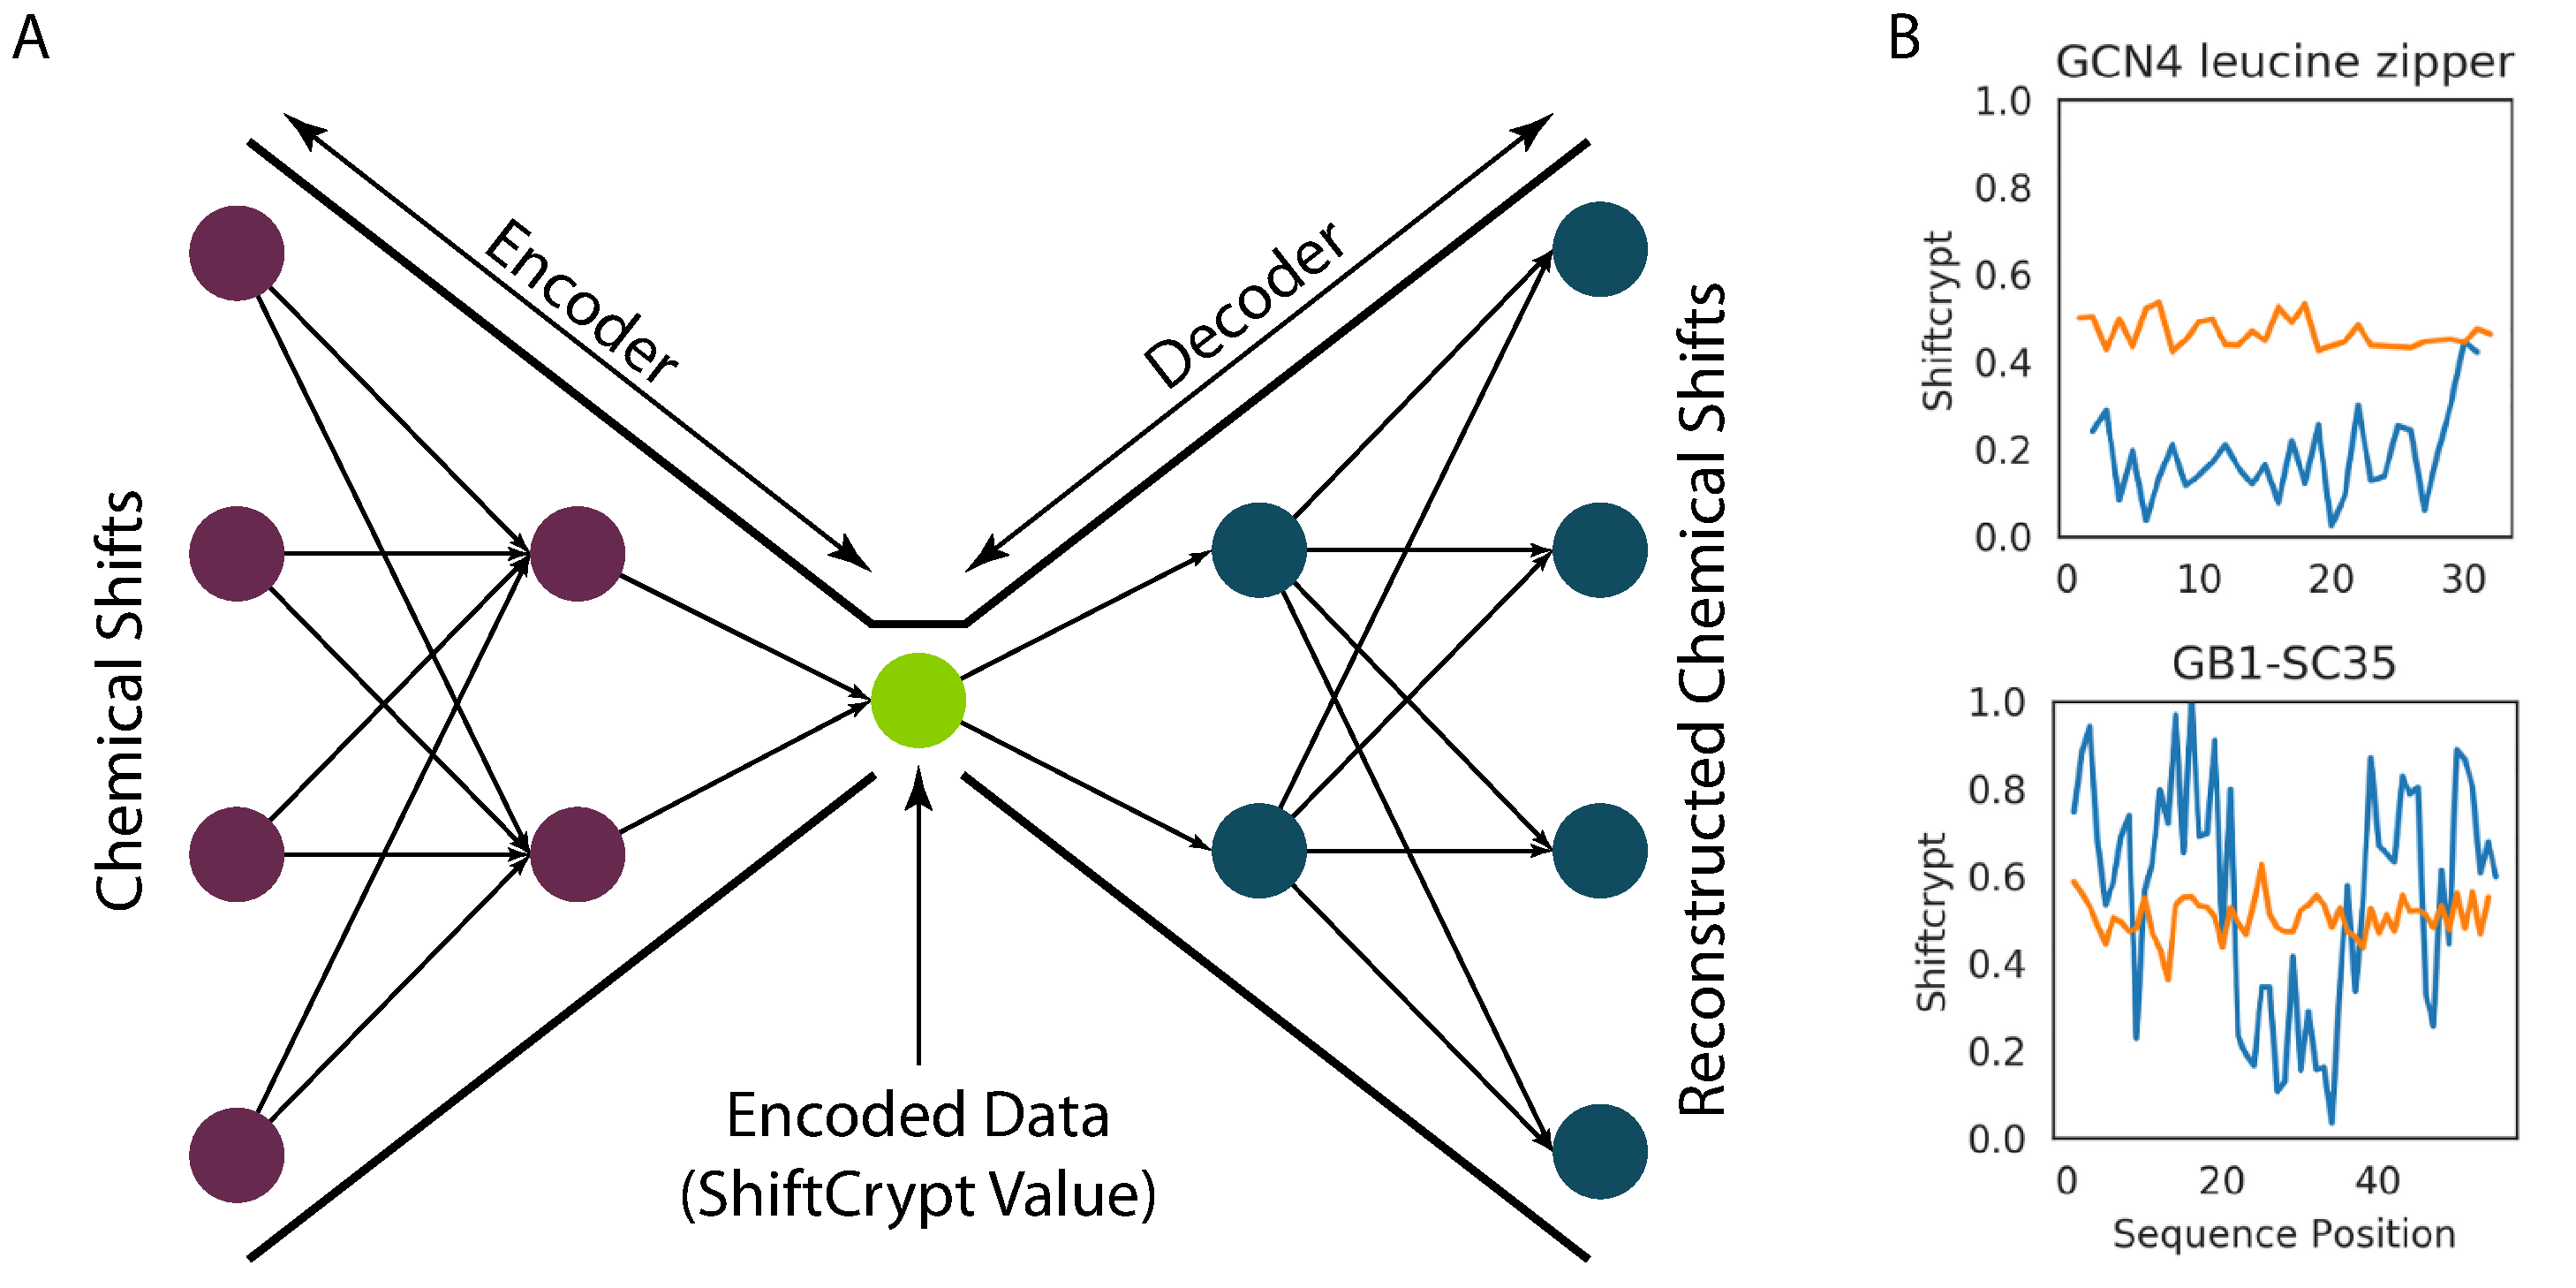
\includegraphics[width=1\linewidth]{figures/shiftcrypt.pdf}
    \caption{\textbf{ShiftCrypt auto-encoder architecture and \gls{proteindisorder} detection.} A) Schematic auto-encoder architecture of ShiftCrypt. The encoder section of the model transforms input \glspl{chemicalshift} into a single encoded value: the ShiftCrypt value. The decoder section of the model attempts to reconstruct the input \glspl{chemicalshift}. B) ShiftCrypt value for two proteins in presence (orange) and absence (blue) of urea. High concentrations of urea effectively denature a protein and causes to adopt a \glspl{proteindisorder} \gls{conformation}. For both proteins, the samples exposed to urea featured near 0.5 ShiftCrypt values, whereas the samples in absence of urea had more extreme values. This indicates that ShiftCrypt can detect absence and presence of fold, respectively. Subplot B extracted from \cite{orlando_shiftcrypt_2020}.}
    \label{fig:chapter1:shiftcrypt}
\end{figure}


\section{AlphaFold and its Relationship with Dynamics}

Over decades, the combined efforts of the structural biology community painstakingly elucidated individual \glspl{proteinstructure}, has resulted in the deposition of over 220,000 \glspl{proteinstructure} in the Protein Data Bank \cite{noauthor_pdb_nodate}. Due to the difficulties in obtaining such data, \gls{proteinstructure} prediction became a prominent field of bioinformatics, with bi-annual editions of the Critical Assessment of Structure Prediction (CASP) judging the state of the field \cite{moult_large-scale_1995}. During CASP, a set of protein sequences with experimentally elucidated but unpublished structures is given to all participants. The predictions from all participants are scored on the prediction of 
protein structures belonging to different categories, according to the protein's difficulty and/or characteristics. This allows to determine which predictive methods work better for each predictive task and quantify their prediction's quality.

Traditionally, protein structural prediction relied on diverse knowledge-based or empirical methods based on statistical and computational techniques, often used in combination. One of these techniques is fragment assembly, where the protein's \gls{aminoacid} sequence is divided into short fragments, typically 3-9 residues long. These fragments are then matched with similar sequences in a database of known \glspl{proteinstructure} to find possible \glspl{conformation} \cite{rohl_protein_2004}. The chosen fragments are assembled into a full \gls{proteinstructure} using an optimisation algorithm to minimise an energy function, which ensures the most likely stable \gls{conformation}. One of these algorithms is the optimisation by \glspl{montecarlosimulations}, a technique that uses random sampling to explore possible configurations and energies of the protein \cite{rohl_protein_2004}. One of the simplest manners to apply \glspl{montecarlosimulations} for \gls{proteinstructure} determination is to randomly change the location of an \gls{aminoacid} and evaluate the free energy of each derived structure. In replica exchange \glspl{montecarlosimulations} \cite{xu_ab_2012}, a series of \glspl{montecarlosimulations} are performed in parallel at different temperatures. The samples are exchanged among different temperatures, which allows for searching an energy \gls{globalminima} at low temperatures and overcome \glspl{localminima} (\figref{fig:chapter1:landscape}) at high temperatures, thereby finding a lower energy minimum solution for the \gls{proteinstructure} \cite{xu_ab_2012}. These simulations require an initial structure to sample, which can be a random coil in its most naïve form or an expected nearer \gls{conformation}, like the \gls{conformation} of a homologous protein or a predicted \gls{conformation} obtained from the previously explained fragment assembly \cite{yang_i-tasser_2015}.


Then, DeepMind's AlphaFold brought a \gls{machinelearning} approach to the assessment, profiting from Protein Data Bank and UniProt databases to train their model \cite{senior_improved_2020}. Two years later, it achieved near-experimental resolution \cite{jumper_highly_2021} for monomeric structures. The large size of the databases employed to create its training set permitted the use of \glspl{deepneuralnetworks}(DNN), which feature multiple high-dimensional layers, generally with complex architectures and activation functions.


AlphaFold2 used both protein sequence and structure data for its training. It used all then available sequences on UniProt, which were filtered for redundancy and aligned in Multiple Sequence Alignments (\gls{msa}). It also generates a pair representation, a matrix with vectors describing the relationship of each \gls{aminoacid} in the input protein with every other \gls{aminoacid}. Both of these were employed to train a series of \gls{attention}-based modules named ``Evoformers'' \cite{vaswani_attention_2023,jumper_highly_2021}, essential for understanding secondary structure elements like \glspl{alphahelix} and \glspl{betasheet}, or structures spanning distant regions, due to the different focus ranges employed (\textit{i.e.} it learns both short- and long-range interactions). In the \gls{msa}, \gls{attention}, an 
advanced feature extraction \gls{machinelearning} method, is applied across the totality of a single sequence to capture patterns within a protein itself, and across a single position in all proteins in the \gls{msa} to capture evolutionary relationships in all aligned proteins. In the pair representation, 2-dimensional \gls{attention} is employed to learn local and global geometric interactions among all \glspl{aminoacid}. This is followed by structure modules, which estimate the protein's 3-dimensional structure from the output of the Evoformer, which is compared with the reference PDB structure during the training process. This process is refined by recycling the data and feeding it back into the network three times (by default), so structural (from PDB) and evolutionary (from \gls{msa}) information is interconnected \cite{jumper_highly_2021} (\figref{fig:chapter1:af2_structure}).



The predicted structures are accompanied by two quality metrics: the predicted local distance difference test (\gls{plddt}) and the predicted aligned error (\gls{pae}). \gls{plddt} is a local metric of predictive confidence expressed as a single value per \gls{aminoacid}, whereas \gls{pae} is a 2-dimensional matrix that indicates the certainty of two residues to be predicted at a correct distance from each other \cite{jumper_highly_2021}. \gls{plddt} was studied as part of this thesis, in relation to different metrics of protein \gls{dynamics}, in chapter \ref{chapter:plddt}, for which we concluded that high and low \gls{plddt} values tend to correlate with protein \gls{flexibility} and \gls{dynamics}, but their gradations are not accurately predicted by \gls{plddt} values. 

Importantly, only the PDB structures obtained from \gls{xraycrystallography} crystallography and \gls{cryoem} were used for training, and any \glspl{ligand} were removed pre-training. This decision results in two important considerations: firstly, the exclusion of \gls{nmr}-derived structures biases the predictions towards more rigid \glspl{conformation} that a protein would obtain in \gls{physiologicalconditions}. Secondly, the removal of \glspl{ligand} results in predicted structures with empty chemical pockets, whose rigidity can be overestimated to the extent that derivative models are able to place the missing \gls{ligand} \cite{hekkelman_alphafill_2023}.

The third iteration of AlphaFold has recently been released \cite{abramson_accurate_2024}, which now allows for the inclusion of ions, small molecules, nucleic acids, and modified \glspl{aminoacid} in the predictions. It also shows improvement in protein complex prediction compared with its previous version. We show in chapter \ref{chapter:plddt} that the relation of AlphaFold3 \gls{plddt} of the $\alpha\text{-carbon}$ with protein \gls{dynamics} and \gls{flexibility} is comparable to that of AlphaFold2 for a reduced set of proteins. We were unable to perform the full large-scale analysis for AlphaFold3, as DeepMind had unfortunately not released the model's source code \cite{noauthor_alphafold3_2024} until days before the submission of this thesis \cite{callaway_ai_2024} and the stringent submission caps to their servers prevented such analysis. This contrasts with the open science requirements that journals have enforced in recent years and has left the community disappointed with Nature's non-enforcement for this specific case \cite{lin_alphafold_2024, wankowicz_alphafold3_2024}.


\begin{figure}[H]
    \centering
    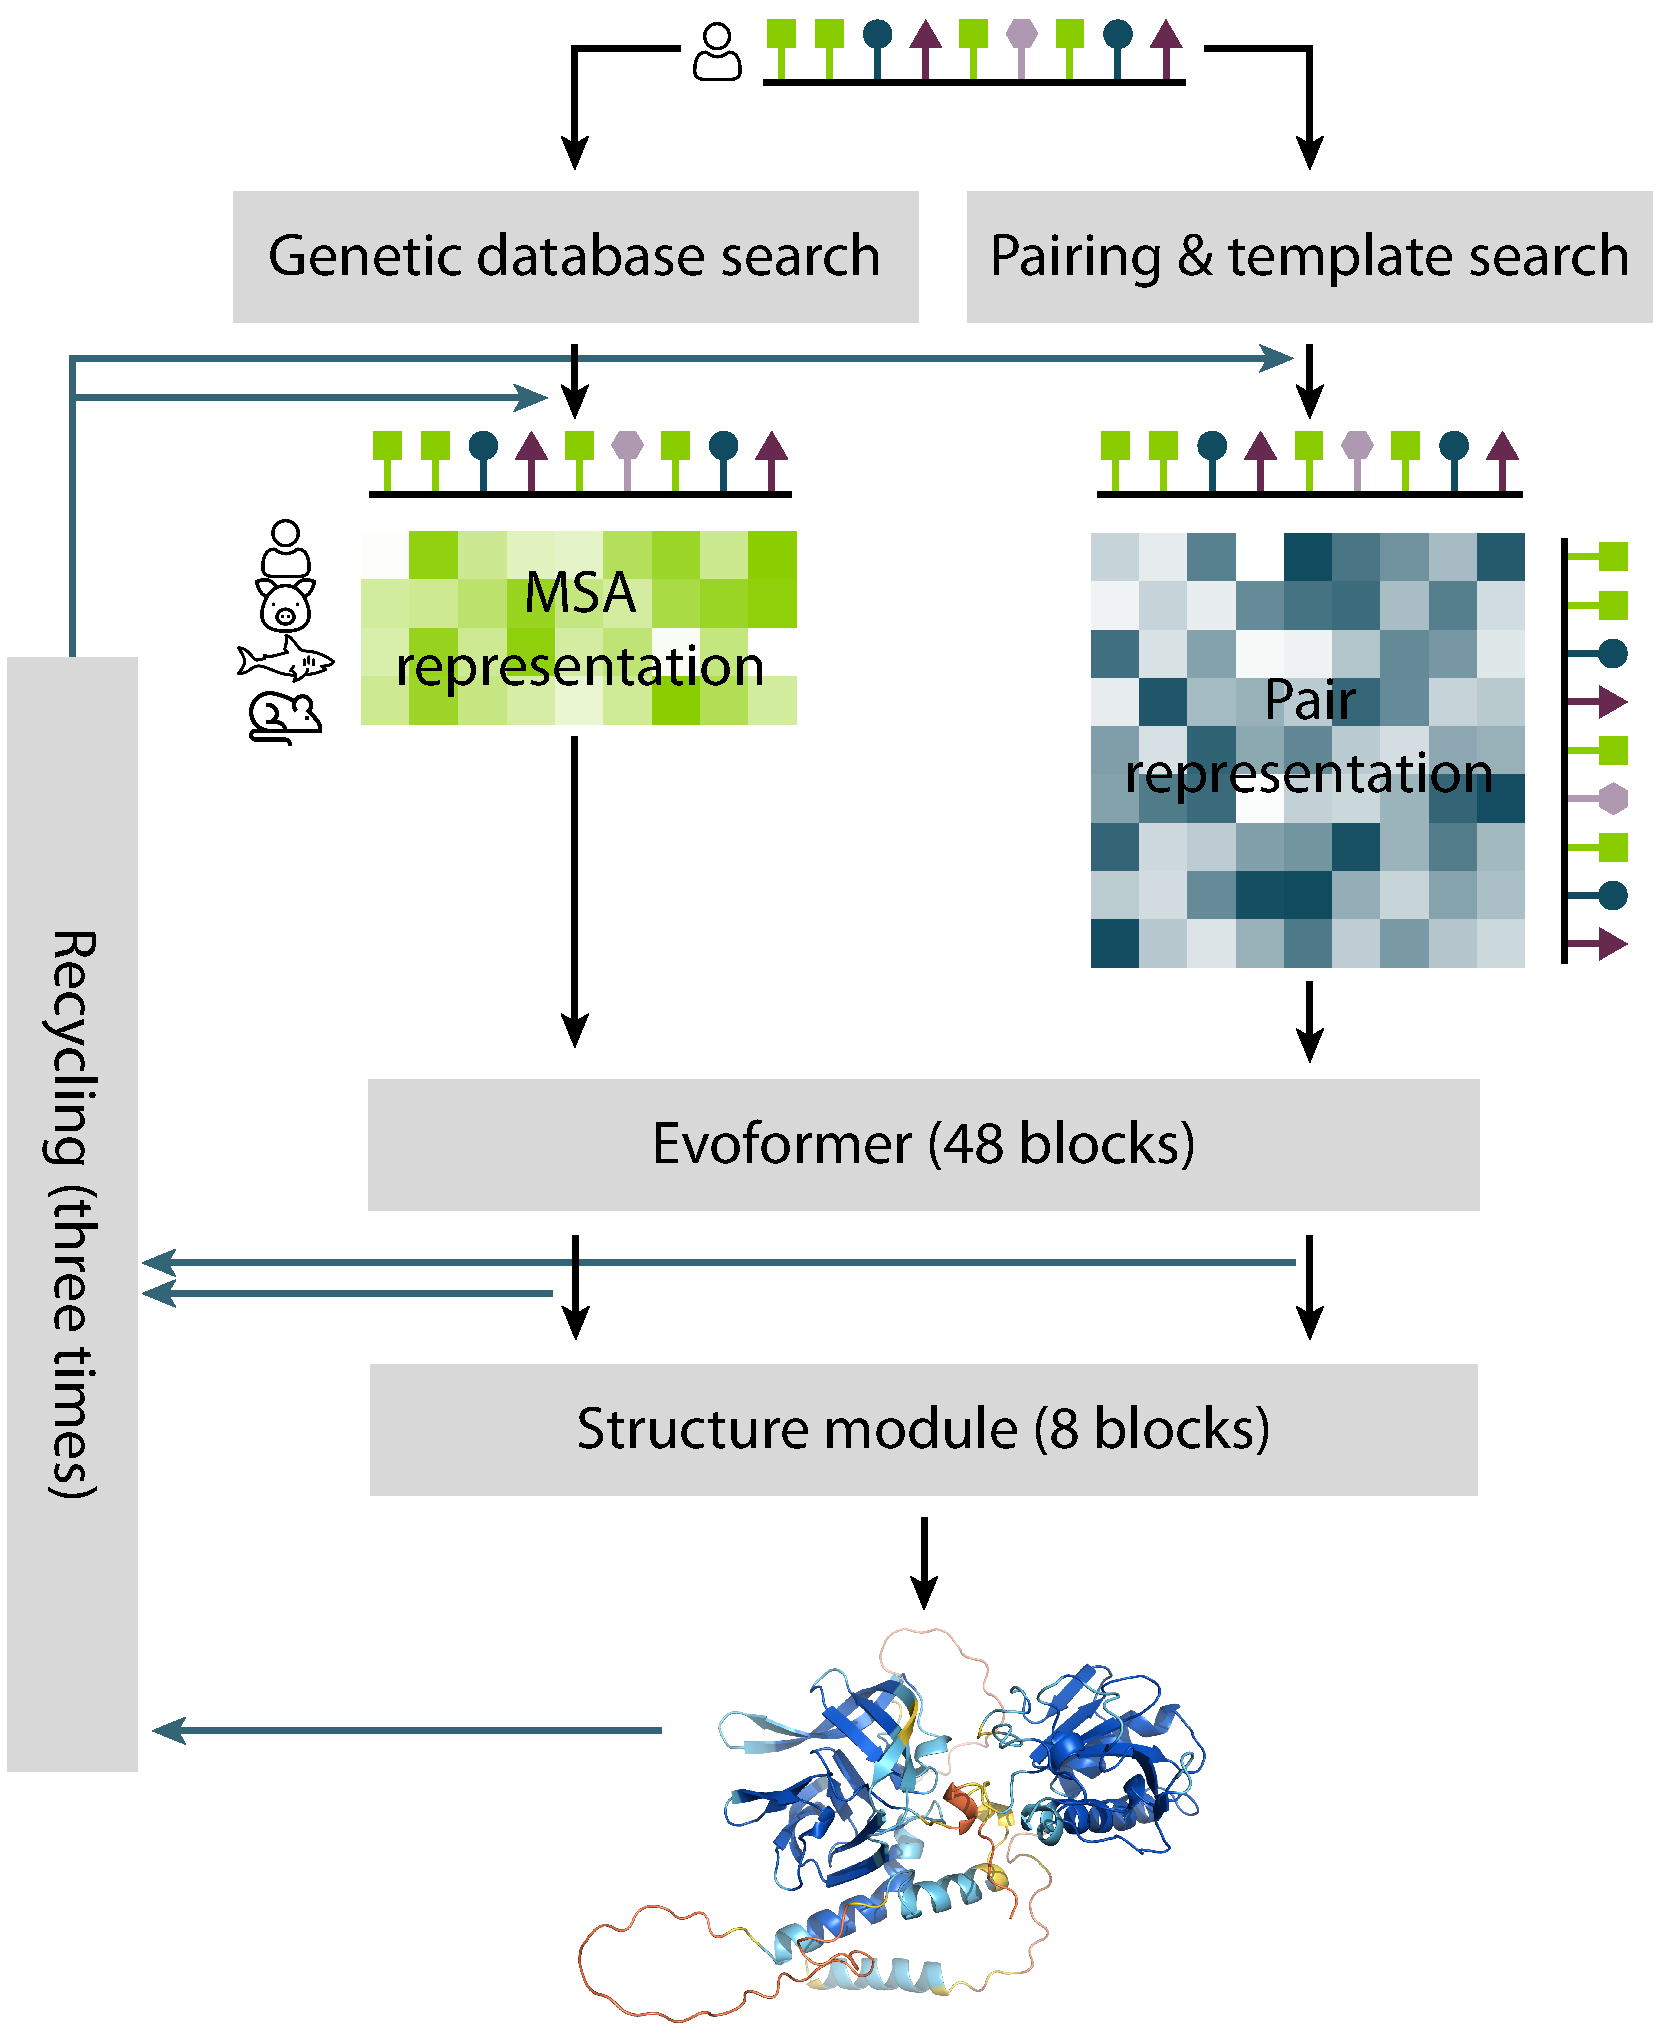
\includegraphics[width=0.75\linewidth]{figures/af2_architecture_simple.pdf}
    \caption{\textbf{AlphaFold2's \gls{neuralnetworks} simplified architecture and training process.} AlphaFold2 takes a protein sequence as input, a human sequence in this example. This sequence is queried against a sequence database to find homologous sequences and align them and create an \gls{msa} representation (left, green matrix). It is also used to create a pair representation (right, blue matrix) and to query a structural database to find suitable templates to facilitate structural modelling (not shown in figure). Both representations are passed through 48 \gls{attention}-based Evoformer blocks, followed by 8 structure module blocks. This produces a predicted structure. The outputs from the Evoformer and structure module blocks are recycled and fed into the \gls{msa} and pair representation 3 times, to refine the results. Figure adapted and simplified from \cite{jumper_highly_2021}. \gls{proteinstructure} downloaded from \burl{https://alphafold.ebi.ac.uk/}, id Q15465. Human and animal icons licensed by \burl{https://www.flaticon.com}.}
    \label{fig:chapter1:af2_structure}
\end{figure}



\section{Open Science and Tool Deployment}

Science has become increasingly open, particularly in the last decade, in order to fight the still ongoing crisis of reproducibility and to ensure that data, tools and methods developed during a project can be used beyond publication day. Funding institutions like the European Commission now require the open publication of derived data, publications, and any other research outcomes. Following this trend, most scientific journals now also require the public deposition of a project’s code and data before even considering publication, with the recent exception of Nature, which did not enforce such requirements by the publication date of DeepMind’s AlphaFold3  \cite{noauthor_alphafold3_2024}.

As a result of science’s move towards greater openness, the FAIR principles (\Gls{findability}, \Gls{accessibility}, \Gls{interoperability}, and \Gls{reusability}) were postulated to allow data have a second life beyond publication \cite{jacobsen_fair_2020}. Not every data set can fully comply with all principles (\textit{e.g.} there is no standard database to collect the specific kind of generated data), but the aim should be to achieve the highest possible compliance. To facilitate this, tools like ELIXIR's Data Stewardship Wizard \cite{pergl_data_2019, devignes_experiences_2023} have been published, which encourage researchers to plan and evaluate their research data management plans to maximise their FAIR score.

Nowadays, these principles are applied not only to data but have also expanded into \glspl{machinelearning} models, manuscripts, and scientific software development. Chapter \ref{chapter:b2btools_deployment} illustrates the efforts made in this thesis to improve the FAIR status of our group's suite of protein biophysical predictors, bio2Byte Tools \cite{gavalda-garcia_bio2byte_2024}. 

% \section{Before you read the remainder of this thesis}
% The work in this thesis is the culmination of 5 years of research at the bio2Byte group, under Wim Vranken's supervision. Following this introduction, I discuss the scientific and societal context of this work, together with my personal contributions to each project in this thesis. This is followed by a collection of articles produced during this period, which represent the main work of the thesis. The vision of the bio2Byte group has clearly influenced me as a researcher, and by extension the contents of this thesis, and one key, unifying concept must be kept in mind for its full understanding: proteins are dynamic entities with no single, static conformation.

% Enjoy the read.

\newpage
% \chapter{Context and scientific contributions of this thesis}\label{chapter:contributions}
\chapter{Context and contributions of this thesis}\label{chapter:contributions}
\chaptermark{Scientific Contributions}
\newpage
\mbox{}
\newpage

The work in this thesis (\figref{fig:chapter2:overview}) began in late 2019, at the dawn of big data for structural biology with the first AlphaFold version \cite{senior_improved_2020}, but before its second version was able to predict most monomeric protein structures from structure at near-experimental resolutions \cite{jumper_highly_2021}. By then, two main voices summarised the state of structural biology: The first believed that the jump in performance for protein structure predictor was due to the change of approach and the inclusion of big data, but the expected evolution of the field would follow previously observed increments. The second believed that the final fold of a protein would soon be predicted from its sequence alone, and structural biology will have to move to different aspects of the protein folding problem \cite{alquraishi_alphafold_2018}, such as the protein \gls{foldingpath}, adoption of multiple \glspl{conformation}, and \gls{dynamics} \cite{powers_proteome_2021}. Just two years later, the latter was proven right when AlphaFold2 predicted protein structures with near-experimental accuracy. The work in this thesis contributes to the study of the remaining elements of the protein folding problem by providing metrics and software to quantify protein \glspl{conformationalensemble} and protein biophysical properties. It also contextualises AlphaFold's models in relation to the metrics here defined and in relation to previously-existing experimental and computational metrics of \gls{dynamics}.

\begin{figure}[tbh!]
    \centering
    \includegraphics[width=\linewidth]{figures/overview_chapter2v2.pdf}
    \caption{\textbf{Overview of projects in this thesis.}
    This thesis keeps the dynamic nature of protein at its core, represented by the central NMR ensemble in this figure (PDB ID: 6V5D \cite{smith_enhancing_2020}). Chapter \ref{chapter:constava} introduces the novel method Constava, which produces residue-level probabilistic propensities of NMR-based conformational states as well as the capability of a residue to exist in multiple of them. Chapter \ref{chapter:b2btools_deployment} describes the path followed to unify the deployment of some of bio2Byte's most popular predictors into a single software suite: b2BTools. In chapter \ref{chapter:ambiguous}, the predictions from these tools are employed as features for a model to produce a residue-level biophysical interpretation order, disorder and ambiguity. Finally, chapter \ref{chapter:plddt} shows the relationship between AlphaFold2's pLDDT and protein dynamics, highlighting some novel nuances in their relationship (AlphaFold2 structure downloded from \burl{https://alphafold.ebi.ac.uk/entry/P0CG48}) 
    }
    \label{fig:chapter2:overview}
\end{figure}

The SARS-CoV-2 pandemic made the scientific community as a whole evaluate how they could contribute in the fight against the virus. In a team effort, the bio2Byte group employed our set of developed tools to estimate the biophysical properties of the virus' proteome. We also estimated these properties for each homologous protein and aligned them in a Multiple Sequence Alignment (\gls{msa}). The aligned predictions showed a biophysically-allowed space for each region, with narrower ranges indicating highly conserved properties and therefore potential targets to disrupt the normal function of a protein. These predictions were made publicly available in a web resource for its immediate availability and later published, now available in this thesis as part of chapter \ref{chapter:b2btools_deployment}. For this publication, I participated in selecting homologous proteins, creating \gls{msa}, and generating and formatting of the predictions, in addition to writing the corresponding section of the manuscript and testing the web resource.  

This effort made us realise that our tools were not as easy to deploy as a whole as we thought at the time. We then started working on the update of our tools, standardization of outputs, and their integration under a single suite: bio2Byte Tools. This suite was first offered as a web service (b2BTools server), which allowed execution either via user interface of Application Programmatic Interface (\gls{api}). This resource allowed the display of all bio2Byte Tools-derived biophysical predictions of a protein in a single view. It also allowed the visualisation of biophysically-allowed space, calculated from predictions calculated from a \gls{msa}. For this work, I directly contributed to the update of the tools.

We then decided to upgrade the deployment of our tools to match higher, more modern standards, and transformed bio2Byte Tools into a Python package. This firstly required the update of all tool's code, models, and dependencies. Then, the execution of the tools was interfaced in a wrapper object, which allowed simpler and unified execution of all tools. The Python package enables both direct interoperability of the obtained results or its storage in \textit{JSON}, \textit{CSV} or \textit{TSV} formats. With every update of the package, the results and execution are now thoroughly tested to ensure no deviation beyond floating point errors occur. The package is subsequently deployed in a variety of channels for both programmatic and non-programmatic usage, namely PyPI \cite{pypi}, Bioconda \cite{gruning_bioconda_2018}, Biocontainers \cite{da_veiga_leprevost_biocontainers_2017}, Galaxy Europe \cite{afgan_galaxy_2018} and in a set of in-house built Docker images (\href{https://hub.docker.com/r/bio2byte/b2btools}{https://hub.docker.com/r/bio2byte/b2btools}). This process is described in further detail in chapter \ref{chapter:b2btools_deployment} \cite{gavalda-garcia_bio2byte_2024}. 

Our work transformed this suite from being a collection of individual tools, with their own dependencies and environments, to being a single unified package, compliant with the FAIR principles. This now allows our suite to be \textit{\Glspl{findability}} and \textit{\Glspl{accessibility}} in different deployment channels \cite{pypi, gruning_bioconda_2018}, archived in Biocontainers \cite{da_veiga_leprevost_biocontainers_2017}, and interfaced on Galaxy Europe \cite{afgan_galaxy_2018} for non-programmatic usage. It also features an \textit{\Glspl{interoperability}} output in standardised formats. Finally, bio2Byte Tools is \textit{\Glspl{reusability}} beyond any dependency, with the creation of Docker containers, insensitive to any future dependency changes. For this work, I developed, implemented and validated the software suite and Continuous Integration and Continuous Deployment (\gls{cicd}) pipelines in close collaboration with Adrian Díaz, and lead the writing of the manuscript (Chapter \ref{chapter:b2btools_deployment}) \cite{gavalda-garcia_bio2byte_2024} and creation of figures. 

Before the final deployment of bio2Byte tools, an earlier version of the tools was employed as part of an assessment to describe proteins with ambiguous behaviour (chapter \ref{chapter:ambiguous}) \cite{roca-martinez_challenges_2022}. My contribution to this analysis is featured in the analysis of AlphaFold2's \gls{plddt} metric for local predictive confidence in relation to bio2Byte's estimations of protein biophysics. The relation between predicted metrics and \gls{plddt} indicated a relationship between highly dynamic regions and and low AlphaFold2 predictive confidence. This relation was shown more clearly when the residues were stratified according to curated order preferences, available in the generated datasets for this work \cite{roca-martinez_challenges_2022}. This work showed the need for a more in-depth analysis of the relationship between \gls{plddt} and protein biophysics, with focus on experimental metrics of protein \gls{dynamics} and \gls{flexibility}. 

In chapter \ref{chapter:plddt} \cite{gavalda-garcia_gradations_2024}, we show a large-scale analysis of AlphaFold2's models in relation to \gls{nmr}-derived \glspl{conformationalensemble} and metrics and diverse computational descriptions of \gls{dynamics} and conformational heterogeneity. For this analysis, I performed the work in relation to metrics derived from \gls{nmr} and Molecular Dynamics, data integration, creation of the code repository and its associated docker image to reproduce the analysis, and I equally contributed with Adrian Díaz to build the interactive analysis in the web server. Bhawna Dixit produced the entirety of the \glspl{nma} for the proteins' AlphaFold2 models and, when available, their \gls{nmr} \glspl{conformationalensemble}. We concluded that AlphaFold2's low \gls{plddt} values tend to co-occur with highly dynamic regions, and so the opposite was true with high \gls{plddt} values and low \gls{dynamics}. This metric, however, was unable to describe gradations in \gls{dynamics}. 

We could also observe that biases on the training set, derived from the removal of ligands from the protein structures, contributed to an overestimation of protein regions rigidity, illustrated by high \gls{plddt} contrasting with \gls{nmr}-assessed dynamic regions. The analysis also showed distinct \gls{plddt} distributions for residues which adopt different conformational states. Interestingly, residues in a relaxed Sheet conformational state (chapter \ref{chapter:constava} \cite{gavalda-garcia_data-driven_2024}) displayed higher \gls{plddt} than those in a stable Helix \gls{conformation}. We hypothesise that such difference originates in the stronger evolutionary signal required to predict Sheet \glspl{conformation} due to the long-range hydrogen bonds required to stabilise this secondary structure, and acquired in AlphaFold2 in its \gls{msa} modules. Helix \glspl{conformation}, on the other hand, are stabilised by near-local, periodic hydrogen bonds, which we argue that permits more \gls{flexibility} in its amino acid sequence and subsequently a weaker signal from the \gls{msa} modules. 

We also find that residues with diverse \glspl{conformation} in their \gls{nmr} \glspl{conformationalensemble} follow lower \gls{plddt} distributions than their unique \gls{conformation} counterparts (Chapter \ref{chapter:plddt}, Supplementary Fig. 5.10). This difference is further accentuated when the secondary structure between \gls{nmr} \glspl{conformationalensemble} and AlphaFold2 models mismatches (Chapter \ref{chapter:plddt}, Supplementary Fig. 5.11). We observe a notable behaviour in residues with an \gls{nmr}-derived consensus \gls{alphahelix} or \gls{betasheet} assignment: i) The match in consensus \gls{nmr} and AlphaFold2 secondary structure assignments for residues without a unique \gls{nmr} assignment results in higher \gls{plddt} distributions than for ii) those with a unique \gls{nmr} assignment which mismatches with AlphaFold2's assignment (Supplementary Fig 5.11, A \& J). 

Residues with a high propensity to acquire a secondary structure, but able to exist in other \glspl{conformation}, will potentially be present in AlphaFold2's training set only in their rigid \gls{conformation}, therefore resulting in high \glspl{plddt}. This is due to the further stabilisation of these structures in the experimental conditions for \gls{xraycrystallography} crystallography or \gls{cryoem}. The existence of Helix and Sheet residues with unique \gls{nmr} assignments which mismatch AlphaFold2's assignments are most likely explained by \gls{folduponbinding} regions, stabilised in the training data set by their ligands, which are then removed. 

This \gls{folduponbinding} is further suggested by the homologous distributions for \gls{nmr}-assigned Coil and Turn residues, which feature higher \gls{plddt} values for residues with unique \gls{nmr} assignments that mismatch with AlphaFold2 than for residues with non-unique \gls{nmr} assignments with matching AlphaFold2 assignment (Supplementary Fig 5.11, D \& G). This indicates higher predictive confidence in residues which acquire a defined, stable structure upon binding over residues which can exist in multiple \glspl{conformation} in their unbound state. Overall, this analysis indicated that the inclusion of only static structures and the removal of binding from AlphaFold2's training set results in difficulties in the assessment of regions that can adopt multiple \glspl{conformation} or fold upon binding. 

Keeping in mind the challenge in representing protein \gls{conformation} from a dynamic perspective, we developed Constava (Chapter \ref{chapter:constava}), a method to measure the capacity of protein residues to exist in multiple conformational states, and how often it transitions among them \cite{gavalda-garcia_data-driven_2024}. This is the result of a close collaboration with Dr. David Bickel to develop, validate and understand the data-driven, probabilistic definition of conformational states propensities and conformational state variability. To achieve this, six conformational states (\textit{Core Helix}, \textit{Surrounding Helix}, \textit{Coil}, \textit{Turn}, \textit{Surrounding Sheet}, and \textit{Core Sheet}) were defined as \glspl{pdf}s in the backbone dihedral space. ShiftCrypt-interpreted \gls{nmr} chemical shifts \cite{orlando_shiftcrypt_2020} values were employed, in combination with STRIDE \cite{frishman_knowledge-based_1995} secondary structure assignments of all models in our experimental \gls{nmr} data set, to identify suitable amino acids to train each of the six \glspl{pdf}s. These conformational states reflect the dynamism of protein structures better than methods designed to be applied to static structures.


Constava leverages information from a collection of static structures, such as \gls{md} trajectories, to derive a continuous probabilistic description of local \textcolor{red}{backbone} \gls{dynamics}, in the form of conformational state variability, and conformational preferences, as conformational state propensities. A sliding window approach is recommended for time-series data, such as \gls{md} trajectories, but bootstrapping is also allowed over a ensemble of structures with no relation between adjacent elements, which enables its usage on \gls{nmr} \glspl{conformationalensemble}. Our results also show that Constava can detect a region's propensity to adopt a certain \gls{conformation} before it fully emerges in an \gls{md} simulation. This has potential applications in \gls{md} simulations, informing about a potentially insufficient sampling of a protein's \gls{conformation}, It can also be applied to protein design, as it can detect regions that could adopt a certain \gls{conformation} if a neighbouring amino acid is substituted to boost that dormant propensity. Overall, Constava offers a new set of metrics to probabilistically describe a protein as the biophysically allowed range of \glspl{conformation} in which it can exist.




% List of articles
\chapter*{Thesis structure}
\addcontentsline{toc}{chapter}{Thesis structure}
\markboth{Thesis structure}{}


The work presented in this thesis is the culmination of five years of research conducted within the bio2Byte group, under the supervision of Wim Vranken. The structure of this thesis reflects the primary focus of my research, organised into four chapters corresponding to six published and submitted articles. The vision of the bio2Byte group has significantly influenced my development as a researcher and, by extension, the contents of this thesis. One key, unifying concept threads through this work: proteins are dynamic entities with no single, static conformation.
% Enjoy the read.
 \vspace{0.8 em}
 % \hrule
% \vspace{0.8 em}
% \\
% \vspace{1cm}

\noindent
\textbf{Chapter \ref{chapter:constava}}:
\\
\textbf{Jose Gavalda-Garcia}, David Bickel, Joel Roca-Martinez, Daniele Raimondi, Gabriele Orlando, and Wim Vranken. Data-driven probabilistic definition of the low energy conformational states of protein residues.
\textit{NAR Genomics and Bioinformatics}, 6(3):lqae082, September 2024. 
\vspace{0.8 em}
\hrule
\vspace{0.8 em}
\noindent
\textbf{Chapter \ref{chapter:b2btools_deployment}}:
\\
\textbf{Jose Gavalda-Garcia}, Adrian Diaz, and Wim Vranken. bio2Byte Tools deployment as a Python package and Galaxy tool to predict protein biophysical properties. \textit{Bioinformatics}, 40(9):btae543, September 2024.
\\
\\
Luciano Kagami, Joel Roca-Martínez, \textbf{Jose Gavaldá-García}, Pathmanaban Ramasamy, K.~Anton Feenstra, and Wim~F. Vranken. Online biophysical predictions for {SARS}-{CoV}-2 proteins. \textit{BMC Molecular and Cell Biology}, 22(1):23, April 2021.
\\
\\
Luciano Porto Kagami, Gabriele Orlando, Daniele Raimondi, Francois Ancien, Bhawna Dixit, \textbf{Jose Gavaldá-García}, Pathmanaban Ramasamy, Joel Roca-Martínez, Konstantina Tzavella, and Wim Vranken.{b2bTools}: online predictions for protein biophysical features and their conservation.\textit{Nucleic Acids Research}, 49(W1):W52--W59, July 2021.
\vspace{0.8 em}
\hrule
\vspace{0.8 em}
\noindent
\textbf{Chapter \ref{chapter:ambiguous}}:
\\
Joel Roca-Martinez, Tamas Lazar, \textbf{Jose Gavalda-Garcia}, David Bickel, Rita Pancsa, Bhawna Dixit, Konstantina Tzavella, Pathmanaban Ramasamy, Maite Sanchez-Fornaris, Isel Grau, and Wim~F. Vranken.
Challenges in describing the conformation and dynamics of proteins with ambiguous behavior. \textit{Frontiers in Molecular Biosciences}, 9, August 2022.
\vspace{0.8 em}
\hrule
\vspace{0.8 em}
\noindent
\textbf{Chapter \ref{chapter:plddt}}:
\\
\textbf{Jose Gavalda-Garcia}, Bhawna Dixit, Adrián Díaz, An Ghysels, and Wim Vranken. Gradations in protein dynamics captured by experimental NMR are not well represented by AlphaFold2 models and other computational metrics, July 2024. \textit{bioRxiv}, Pages: 2024.07.17.603933 Section: New Results.

\chapter*{Thesis aims}
\addcontentsline{toc}{chapter}{Thesis aims}
\markboth{Thesis aims}{}

% \begin{enumerate}

%     \item Can we define a protein structure representation that better captures statistical behaviour when multiple conformations are present? 
%     \begin{enumerate}
%         \item To address this....
        
%     \end{enumerate}
%     \item Can we describe this statistical behaviour based on data that more accurately reflects protein behaviour in solution?
%     \item Can AlphaFold’s local metric for prediction confidence (pLDDT) effectively describe ambiguous protein behaviour?
%     \item Do AlphaFold models reflect information obtained from protein NMR ensembles, experimental NMR metrics of dynamics, and interpreted molecular dynamics data?
%     \item Can we identify biases and limitations within AlphaFold models?

% \end{enumerate}

\begin{enumerate}
    \item Coordinate-based representations of proteins are limited when describing proteins that adopt multiple conformations. Even when numerical methods (\textit{e.g.} Root Mean Squared Fluctuations) are employed to describe the flexibility of these regions, they cannot identify conformational change events. To address this: 
    \begin{enumerate}
        \item Can we develop a protein representation that better captures statistical behaviour across multiple conformational states?
        \item Can this statistical behaviour be described using data that more accurately reflects protein behaviour in solution?
        \item Can this representation identify residue-level changes in conformation related to changes in such behaviour?
    \end{enumerate}
    
    \item AlphaFold can produce highly-accurate protein structural models from amino-acid sequence, enabling the structural prediction across whole proteomes. Considering that this method was trained and benchmarked with protein structural models produced under cryogenic conditions: 
    \begin{enumerate}
        \item Does AlphaFold's local confidence metric, pLDDT, effectively capture ambiguous protein behaviour?
        \item Can we identify in AlphaFold models a reflection of protein flexibility and dynamics, measured from protein NMR ensembles, experimental NMR metrics of dynamics, and interpreted molecular dynamics data?
        \item Can biases and limitations within AlphaFold models be identified?
    \end{enumerate}

    \item Our research group, bio2Byte, has developed multiple tools to study different aspects of protein dynamics. While these tools provide complementary predictions of protein dynamics, unified execution was not possible at the start of this thesis due to incompatible requirements and syntax. Considering these limitations: 
    \begin{enumerate}
        \item Can we harmonise these tools into a unified suite to enable seamless execution?
        \item Can we improve the tools' deployment to ensure long-term usability and expand accessibility for users without programming proficiency?
    \end{enumerate}
\end{enumerate}

% Main point is the problem/question. Subpoints are how we're fixing it



% \newpage

\subfile{constava/main_constava}

\chapter{Challenges in describing the conformation and dynamics of proteins with ambiguous behavior.} \label{chapter:ambiguous}
\chaptermark{Ambiguous behaviour}

Joel Roca-Martinez $^{1,2,\dag}$, Tamas Lazar $^{1,3,\dag}$, Jose Gavalda-Garcia $^{1,2}$, David Bickel $^{1,2}$, Rita Pancsa $^{4}$, Bhawna Dixit $^{1,2,5}$, Konstantina Tzavella $^{1,2}$, Pathmanaban Ramasamy $^{1,2,6}$, Maite Sanchez-Fornaris $^{1,2,7}$, Isel Grau $^{8}$, Wim F. Vranken $^{1,2}$.
\\
\\
$^{1}$ Structural Biology Brussels, Vrije Universiteit Brussel, Brussels, Belgium.
\\
$^{2}$ Interuniversity Institute of Bioinformatics in Brussels, VUB/ULB, Brussels, Belgium.
\\
$^{3}$ VIB-VUB Center for Structural Biology, Brussels, Belgium.
\\
$^{4}$ Research Centre for Natural Sciences, Institute of Enzymology, Budapest, Hungary.
\\
$^{5}$ IBiTech-Biommeda, Universiteit Gent, Gent, Belgium.
\\
$^{6}$ VIB-UGent Center for Medical Biotechnology, Universiteit Gent, Gent, \\Belgium.
\\
$^{7}$ Department of Computer Sciences, University of Camagüey, Camagüey, Cuba.
\\
$^{8}$ Information Systems, Eindhoven University of Technology, Eindhoven, \\Netherlands.
\\
\\
DOI: 10.3389/fmolb.2022.959956

\vspace{1em}
\hrule
\vspace{1em}

\begin{abstract}
    Traditionally, our understanding of how proteins operate and how evolution shapes them is based on two main data sources: the overall protein fold and the protein amino acid sequence. However, a significant part of the proteome shows highly dynamic and/or structurally ambiguous behavior, which cannot be correctly represented by the traditional fixed set of static coordinates. Representing such protein behaviors remains challenging and necessarily involves a complex interpretation of conformational states, including probabilistic descriptions. Relating protein dynamics and multiple conformations to their function as well as their physiological context (\textit{e.g.}, post-translational modifications and subcellular localization), therefore, remains elusive for much of the proteome, with studies to investigate the effect of protein dynamics relying heavily on computational models. We here investigate the possibility of delineating three classes of protein conformational behavior: order, disorder, and ambiguity. These definitions are explored based on three different datasets, using interpretable machine learning from a set of features, from AlphaFold2 to sequence-based predictions, to understand the overlap and differences between these datasets. This forms the basis for a discussion on the current limitations in describing the behavior of dynamic and ambiguous proteins.
\end{abstract}

\section*{Author contributions}

JR-M trained the RF models; IG contributed the RF interpretation code; JR-M, TL, RP, PR, and KT contributed datasets; JG-G contributed the analysis of the AlphaFold2 models; KT contributed the analysis of deleterious mutants; PR contributed the analysis of PTMs; WV provided the manuscript concept and organization of results; JR-M, TL, JG-G, DB, BD, KT, PR, MS-F, and WV contributed to the writing.

\newpage

% ========================================
\section{Introduction}
% ========================================

The importance of protein dynamics for their (mis-)folding \cite{daggett_is_2003, dobson_protein_2003} and functionality \cite{karplus_molecular_2005, glazer_improving_2009} has been long recognized, but has been overshadowed by the need to first understand how most proteins fold into well-defined three-dimensional structures (unique conformations) \cite{hunkapiller_contemporary_1984, berman_worldwide_2007}. The recent impressive performance of AlphaFold2 \cite{jumper_highly_2021} in predicting such unique protein folds from i) protein sequence and evolutionary information curated by UniProt \cite{the_uniprot_consortium_uniprot_2021}, and ii) the carefully assembled protein structure information from the Protein Data Bank over many decades \cite{berman_worldwide_2007} indicates that this problem is now largely solved. This also implies that experimental and computational approaches for proteins will now have to necessarily focus beyond their fold, specifically on understanding more about how proteins interact, which alternative conformations they might adopt, and how they move between these conformations. Indeed, many proteins show ambiguous conformational behavior, either in specific regions within folded domains (e.g. loops such as CDRs in antibodies \cite{armstrong_conformational_2008}, or extracellular loops in GPCRs \cite{hilger_structure_2018}), in regions connecting folded domains (e.g. PEVK domain of titin \cite{hsin_molecular_2011}), or the full protein in case of intrinsically disordered proteins (e.g. Phd antitoxin from Bacteriophage P1 \cite{de_gieter_intrinsically_2014}). Systematic studies on ambiguous/disordered proteins have already proved that missing residues in crystal structures do not always correlate with protein disorder, in fact, sometimes are predicted as highly ordered \cite{gall_intrinsic_2007}. Similarly, residues that are present or missing for the same protein in different X-ray structures, are rarely statically disordered and show a partial or conditional disorder under different experimental conditions. This different degree of disorder was previously described and categorized into foldable, non-foldable or semi-foldable regions, where some protein regions undergo a structural rearrangement at a certain point in time, either spontaneously or induced (e.g. after binding with another molecule) \cite{uversky_unusual_2013}. The move from the traditional paradigm, with the sequence encoding for a single static structure, towards a dynamic paradigm, where the sequence encodes for different possible behaviors, also implies the necessity to approach proteins from a probabilistic viewpoint. This is a reasonable assumption, especially when considering that billions of copies of the same protein exist in cells, at thermodynamically high temperatures; all these proteins will have different interactions and (locally) different conformations at any given time point, and might have (different) post-translational modifications \cite{vu_protein_2018}. Such a proteomics-based probabilistic in vivo view of proteins is in stark contrast to the reductionist and static single-protein view in the traditional paradigm.

There have nevertheless been significant efforts in the experimental investigation of the conformational ambiguity and heterogeneity of protein structures and structural ensembles by various techniques: nuclear magnetic resonance (NMR), circular dichroism (CD) and electron paramagnetic resonance (EPR) spectroscopy, small-angle X-ray and neutron scattering (SAXS/SANS), Förster resonance energy transfer (FRET) measurements, electrospray ionization-ion mobility mass spectrometry (ESI/IM-MS) and hybrid approaches that integrate more than one of the above mentioned techniques \cite{dobson_biophysical_2019}. Although X-ray crystallography and cryo-electron microscopy may both be able to trap more than one protein conformer of globular proteins, solution techniques are undoubtedly preferred for uncovering the dynamics of flexible proteins, with NMR being the approach that initially highlighted these features in proteins using different types of measurements (chemical shifts, R1, R2, J-couplings, NOEs, RDCs). Lately, there have also been efforts dedicated to studying the dynamics of flexible and intrinsically disordered proteins (IDPs) in the cellular context using in-cell NMR and EPR spectroscopy, as a protein’s conformational behavior may differ from what is observed in isolation in the test tube \cite{kragelund_-cell_2020, bonucci_crowding_2021}. However, due to various experimental challenges, these methods have not become widely used in the community of structural biology. Valid future alternatives for both single proteins (folding) and in-cell determination of protein states might come from mass spectrometry-based methods such as cross-linking (XL-MS) or hydrogen-deuterium exchange (HDX-MS), which are becoming increasingly informative \cite{britt_integration_2022}.

On the computational side, molecular dynamics (MD) and Monte Carlo (MC) simulations are commonly used to investigate the conformations and/or dynamics of proteins, often in combination with experimental data to either restrain the structure of the protein, or to reweight a pool of structures generated from the simulation trajectory to obtain a conformational ensemble that complies with the experimental readout \cite{lindorff-larsen_simultaneous_2005, hummer_bayesian_2015, childers_validating_2018, orioli_how_2020}. Recent advances in force field (FF) development combined with enhanced sampling techniques now enable more realistic exploration of protein dynamics and flexibility even in absence of experimental data \cite{yang_enhanced_2019, abriata_assessment_2021}. Besides the advances achieved in developing FFs that excel on IDPs (e.g. CHARMM36IDPSFF, Amber ffIDPs and ffIDPSFF) \cite{huang_force_2018, zapletal_choice_2020, mu_recent_2021}, the major focus nowadays is on those achieving a balanced sampling on both folded and disordered proteins (such as CHARMM36m \cite{huang_charmm36m_2017}, Amber ff19SB20 and DES-Amber \cite{piana_development_2020}). The main advantage of these simulations is their capability to account for context-dependency (e.g. temperature, ionic strength, PTMs and a partner), however their disadvantage is their computational cost, which prohibits proteome-wide/large-scale systematic analyses. To this end, various fast and computationally inexpensive sequence-based predictors have been developed, with many focusing on estimating intrinsic disorder. Disorder predictors can be cataloged into three main categories given their underlying prediction model: 1) ab initio methods like IUPred \cite{dosztanyi_iupred_2005}, that are based on the protein’s physico-chemical properties; 2) machine learning algorithms trained on experimental annotations like Disomine \cite{orlando_prediction_2022}, Disopred \cite{ward_disopred_2004}, DisEMBL \cite{linding_protein_2003} and SPOT-DISORDER2 \cite{hanson_spot-disorder2_2019} and 3) the meta-predictors which combine several individual predictors, like PONDR-FIT \cite{xue_pondr-fit_2010}, ESpritz \cite{walsh_espritz_2012}, DISOPRED3 \cite{jones_disopred3_2015}, MFDp2 \cite{kihara_prediction_2014}, and others. Usually, most of these predictors of protein disorder focus on labeling regions of missing electron density as regions of disorder using X-ray crystallography or NMR data, categorizing each residue in only one of two classes, ignoring potentially useful conformational states of the protein. However, there are new predictors that address those kinds of different behaviors, like IUPred2A \cite{meszaros_iupred2a_2018}, ODINPred \cite{dass_odinpred_2020}, DispHred \cite{santos_disphred_2020} assigning a degree of disorder to each amino acid and other predicted features of the protein indicating the amount or degree of disorder like NetSurfP-2.0 \cite{klausen_netsurfp20_2019} that outputs solvent accessibility, secondary structure, structural disorder, and backbone dihedral angles for each residue of the input sequences. The intrinsically semi-disordered state has also been studied, with predictors able to identify such behavior often associated with induced folders and \gls{aggregation}-prone regions \cite{zhang_intrinsically_2013, katuwawala_computational_2019}. In addition, other sequence-based predictors provide useful information, such as backbone dynamics (DynaMine \cite{cilia_protein_2013, cilia_dynamine_2014}), fuzziness (FuzPred \cite{horvath_sequence-based_2020, miskei_sequence-based_2020}), secondary structure (PSIPRED4 \cite{jones_protein_1999}, SPOT-1D \cite{singh_spot-1d-single_2021}), solvent accessibility (SABLE \cite{adamczak_accurate_2004}, ACCpro \cite{magnan_ssproaccpro_2014}, SPOT-1D \cite{singh_spot-1d-single_2021}), solubility / aggregation propensity (TANGO \cite{fernandez-escamilla_prediction_2004}, AGMATA \cite{orlando_accurate_2020}, PASTA2 \cite{walsh_pasta_2014}, CamSol \cite{sormanni_camsol_2015}), liquid-liquid phase separation propensity (catGRANULE \cite{bolognesi_concentration-dependent_2016}, PScore \cite{vernon_pi-pi_2018}, PSPer \cite{orlando_computational_2019}, Droppler \cite{raimondi_silico_2021}) and other biophysical features of proteins. As most of these prediction tools only take the sequence as input, with sometimes a few specificity or sensitivity parameters, they remain largely context independent and cannot take factors such as pH, temperature, or PTMs into account. The exception are a few specific cases such as i) oxidation-dependent disorder prediction by IUPred2A \cite{meszaros_iupred2a_2018}; ii) pH-dependent solubility prediction for IDPs by SolupHred \cite{santos_disphred_2020, santos_ph-dependent_2020, pintado_soluphred_2021}; iii) prediction of molecular recognition features/elements (MoRFs/MoREs) that are interacting regions of IDPs undergoing an increase in the secondary structure propensity upon binding (e.g. $\alpha$-MoRF-PredII predictors \cite{oldfield_coupled_2005, cheng_mining_2007}, MORFchibi \cite{malhis_morfchibi_2016}, SPOT-MoRF \cite{hanson_identifying_2020}, fMoRFpred \cite{yan_molecular_2016}); and iv) experimental condition (pH, temperature, ionic strength, crowding agent, protein concentration)-dependent prediction of liquid-liquid phase separation by Droppler \cite{raimondi_silico_2021}.

Another significant influence on protein behavior is post-translational modifications (\gls{ptms}), which regulate the function, activity and stability of proteins. Several studies have shown the association of PTMs in various diseases, such as cancer, Alzheimer’s and diabetes \cite{mclaughlin_where_2016, song_post-translational_2019, bai_proteomic_2021}. PTMs alter the biophysical, thermodynamic, and kinetic properties of proteins leading to a diverse conformational landscape than dictated by the arrangement of 20 amino acids \cite{shental-bechor_effect_2008}. Therefore, a complete comprehension of a folded protein monomer is useful however insufficient to understand the functioning of a protein in a biological environment. The structural preferences of PTMs are divided into two categories: well-defined secondary structure (N-linked glycosylation, acetylation) and intrinsically disordered regions (phosphorylation, methylation). These PTMs can exist simultaneously in different amino acids (methylation, phosphorylation), or in the same amino acid over time (ubiquitination, phosphorylation) depending on the biological context. The impact of PTMs on protein structures can vary diversely ranging from local conformational stabilization or destabilization of secondary structure elements, to transitions between intrinsically disordered and ordered states \cite{bah_modulation_2016}. 

\begin{figure}[tbh]
    \centering
    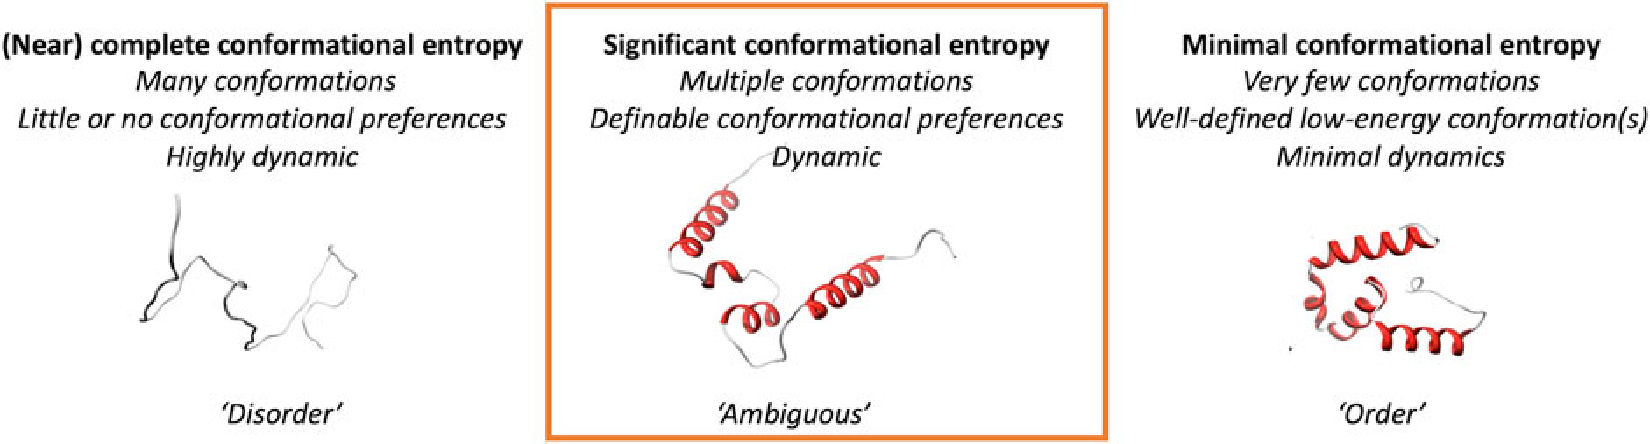
\includegraphics[width=\linewidth]{ambiguous//figures_ambiguous/fig1.pdf}
    \caption{\textbf{Conceptual definition of the “ambiguous” regions of proteins addressed in this study.}}
    \label{fig:chapter5:fig1}
\end{figure}

In the case of IDPs, the disorder-to-order transitions can be considered ``a black box of structural biology''. This multifaceted folding/unfolding behavior is widely regulated and modulated by PTMs. The alteration of IDPs’ conformational space, dynamics, functionality, cellular expression, and localization caused by PTMs can also be unfavourable and cause protein pathogenicity. This equivocal relationship of PTMs and IDPs significantly enlarges the complexity of the black box, which is invisible yet an important attribute of protein folding \cite{bah_modulation_2016}. Currently, the change in conformational dynamics of a protein when modified by a PTM can be investigated by MD simulations. However, systematic force-field parameters required for MD simulations are limited to several PTMs (methylation, phosphorylation, glycosylation) and require optimization and validation, which is computationally expensive. It therefore remains a black box, since the current tools are deficient in terms of exploring PTMs and conformational behavior of proteins. On the other hand, the stability of folded regions can also be affected by PTMs. Incorporating information about PTMs in our understanding of in vivo protein behavior is therefore essential.



We here explore a class of protein regions that are more likely to adopt multiple different conformations and show ambiguous behavior; they can neither be strictly classified as traditional ``order'', nor as the oppositely defined ``disorder'' (\figref{fig:chapter5:fig1}). We focus on three different scenarios of conformational ambiguity: i) regions that undergo ``order-to-disorder'' transitions, where a protein (region) that is disordered folds when encountering a binding partner, ii) regions of folded proteins that can change their conformation, and iii) regions that have ambiguous behavior in solution based on NMR chemical shift information. Such inherent ambiguous behavior could be relevant for conformational changes in the protein, for example upon oligomerization, interacting with another molecule or the cell membrane, or when being post-translationally modified. These changes should happen within the context of biologically reasonable environments and protein modifications, not for example, in disorder-or-order inducing agents such as TFE, or denaturing agents like urea. We here show, based on two different definitions and their joint one, that ambiguous regions are difficult to define, but that combinations of datasets from different sources might help to unravel this complex protein behavior.

\section{Methods}

\subsection{Datasets}

\subsubsection[DisProt ``folding-upon-binding'' Dataset with CoDNaS Dataset]{DisProt ``folding-upon-binding'' Dataset with CoDNaS Dataset (disprot_codnas_set)}

DisProt is a large database of manually curated intrinsically disordered protein (IDP) regions (IDRs) \cite{hatos_disprot_2019}. Besides the structural state and the function of the region, if available, interaction partners and potential structural transitions (e.g. displaying folding-upon-binding) are also annotated for DisProt entries. For the present study, we downloaded a custom set of human proteins with manually curated disorder-to-order structural transitions, resulting in 138 different proteins with at least one IDR that undergoes ordering. The residues that are classified as undergoing structural ordering were labeled as ambiguous (N = 9,792 residues) and the residues in the IDR flanking regions that are not proven to undergo structural ordering were labeled as disordered (N = 4,232 residues). 

CoDNaS \cite{monzon_codnas_2016} stores proteins with multiple X-ray and NMR structures solved under different experimental conditions. The difference between these conformations of ``snapshots'' varies on a wide range: rigid globular structures being on one side of the spectrum and disordered structures on the other side. To assemble a set of rigid proteins, we downloaded structural clusters by applying the threshold of a maximum RMSD value of 2Å for each pair of structures available for the same protein region. This way we obtained a reliable set of 207 human proteins entailing 11,947 residues in ordered segments.

These two datasets were combined into a single dataset, which therefore contains highly reliable definitions for ordered residues (O) for which little or no conformational change has been observed in experimental protein structures (from CoDNaS) as well as disorder (D) (from DisProt) and ambiguous behavior folding-upon-binding residues, with a local change in environment (the binding partner) triggering a conformational transition or rearrangement (T) (from DisProt).


\subsubsection[MFIB Dataset]{MFIB Dataset (mfib_set)}

MFIB \cite{ficho_mfib_2017} is a database of mutually folded IDPs/IDRs that synergistically fold upon binding, while as monomers the protein chains are unstructured. A subset of MFIB was manually selected to reduce the redundancy in terms of sequence-structure relationship. Additional overlap with other datasets has also been filtered out, in total 5 protein chains also part of the DisProt set have been eliminated. The final set of cases include 17 chains from homo- and 23 chains from heterocomplexes forming various types of folds (incl. histone-like folds, basic helix-loop-helix, Phe-, Leu- and Ala-zippers, ribbon-helix-helix folds... etc.), with 1-3 examples selected from each fold category. The complete dataset is available in \burl{https://bitbucket.org/bio2byte/protein_ambiguity/}.


\subsubsection[Metamorphic and Fold-Switching Proteins Dataset]{Metamorphic and Fold-Switching Proteins Dataset\\(foldswitch_set)}

The fold switchers dataset is a manually curated list of pairs of experimentally solved structures for the same protein that showed a different topology in some parts of the sequence. This dataset provides experimental prove of residues that can switch from one secondary structure element type to another one (e.g., a residue that in one of the PDB structures is in an $\alpha$-helix and in the other one is in a $\beta$-strand). The original fold switchers list consisted of 94 protein pairs (PDB entries), but we filtered it to keep only the protein sequences that shared the same sequence, as small sequence variations could have an impact on the protein topology and would therefore affect our study. 29 structure pairs remained totaling 8,047 residues. This dataset is available in \burl{https://bitbucket.org/bio2byte/protein_ambiguity/} as supplementary material.

The residues were labeled using the DSSP secondary structure annotations \cite{kabsch_dictionary_1983} extracted from the PDBe API \cite{mir_pdbe_2018} for each of the structures in the pair. Residues that stayed in either in helix or sheet conformations were labeled as same (S), while residues that switched from any secondary structure type to another one, were labeled as convert (C). We did not use the residues that stayed in coil for this analysis to avoid including likely disordered regions in any of the two forementioned categories. A total of 3,751 and 1,341 residues were labeled as S and C, respectively.


\subsubsection[Combined Dataset]{Combined Dataset (combined_set)}
A new dataset merging the disprot_codnas_set and foldswitch_set was generated by combining some of the categories of the previous ones (combined_set). The ordered (O) and same (S) categories from the disprot_codnas_set and foldswitch_set were merged as they were comparably defined. In both cases the residues that fall into these categories are amino acids that have proved rigid/conformationally stable in several experimental assays. Similarly, the ambiguous folding upon binding residues (T) from DisProt and the fold-switching residues (C) also share a particular biophysical behavior, as in both categories the residues undergo a conformational rearrangement. The goal is to assess whether this dataset exhibits similar features with respect the disprot_codnas_set and foldswitch_set or it captures different biophysical characteristics. The disordered category (D) remains as defined in the disprot_codnas_set. The total number of residues in this set are 15,698, 10,750 and 4,232 for Ordered (O + S), ambiguous (T + C) and disordered (D) respectively.


\subsubsection[PTM Dataset]{PTM Dataset (ptm_set)}

PTM information was obtained from four different resources Scop3P \cite{ramasamy_scop3p_2020}, UniProtKB/Swiss-Prot \cite{the_uniprot_consortium_uniprot_2021}, dbPTM \cite{huang_dbptm_2019} and PhosphoSitePlus (PSP) \cite{hornbeck_phosphositeplus_2015}. Scop3P annotates protein phosphorylation sites by re-processing large scale public proteomics datasets. dbPTM integrates experimentally validated PTM sites from Swiss-Prot, PhosphoELM and O-GLYCBASE. UniProtKB includes PTM information that is directly curated from scientific literatures and propagates the information to homologues. PSP contains manually curated PTM information obtained from literature. We downloaded PTM information from all the above-mentioned resources (April 2022). All the obtained PTM sites were checked for the correctness in sequence positions with the current UniProtKB/Swiss-Prot human protein sequences. To obtain a reliable set of PTM sites, we only considered sites having at least two different database evidence. Sites having more than one PTM type are labeled as ``multiple''. The final dataset contains 217082 PTM sites from 15,420 canonical human proteins. The complete data table is available from \burl{https://bitbucket.org/bio2byte/protein_ambiguity/}.


\subsubsection[AlphaFold Human Proteome Dataset]{AlphaFold Human Proteome Dataset (af_set)}
AlphaFold 2’s mmCIF files for the human proteome were downloaded on September 2nd 2021 from the AlphaFold protein structure database \cite{tunyasuvunakool_highly_2021}. In this section, we will refer to this dataset as ``AF_dataset''. According to AF_dataset’s description page \burl{https://alphafold.ebi.ac.uk/download}), sequences longer than 2,700 residues were split in multiple files. For simplicity, we removed these sequences and kept only sequences contained in a single file. Then, we extracted the protein ID, sequence, pLDDT and secondary structure, simplified to alpha_helix, beta_strand and all remaining conformations were labeled as coil. 

We also downloaded all human Swiss-Prot entries contained in Uniref90 \cite{suzek_uniref_2007} on September 2nd 2021 from UniProt \cite{the_uniprot_consortium_uniprot_2021}. In this section, we will refer to this dataset as ``uniref_dataset''.  From this set, we discarded all proteins shorter than 20 amino acids, since some of our predictive tools have this minimum length requirement. Then, we found the sequences intersection between AF_dataset and uniref_dataset and verified that the sequences in both sets were correctly aligned, which resulted in the ``selected_human_dataset''. 

With these sequences, we computed sequence-based predictions with the b2btools predictors, comprising DisoMine (disorder) \cite{orlando_prediction_2022}, DynaMine (backbone \cite{cilia_protein_2013} and side-chain dynamics, conformational propensities \cite{raimondi_exploring_2017}), EFoldMine (early folding propensity) \cite{raimondi_exploring_2017} using a recently developed PyPI package currently in open beta (\burl{https://pypi.org/project/b2bTools/3.0.0b16/}). We then merged our predictions with the mLDDT and secondary structure predictions that we extracted from AF_dataset into our selected_human_dataset. Finally, our selected_human_dataset was saved into a Numpy file for later processing and can be found in \burl{https://bitbucket.org/bio2byte/protein_ambiguity/}.


\subsubsection{Deleterious Mutant Datasets}
Even though mutation is a random process, it frequently occurs at highly conserved hotspots of the protein which represent regions of structural and functional importance \cite{chang_accelerating_2018}. To explore the definition of Ambiguous regions, we downloaded publicly available deleterious somatic mutations from Catalogue Of Somatic Mutations In Cancer (COSMIC version 92_1121) \cite{forbes_catalogue_2008} and Cancer Genome Interpreter \cite{tamborero_cancer_2018} and germline deleterious and benign mutations from ClinVar \cite{landrum_clinvar_2018} and UniProtKB/Swiss-Prot \cite{the_uniprot_consortium_uniprot_2021} respectively. The COSMIC database contains more than 13 million mutations associated with various cancer types. UniProtKB/Swiss-Prot contain variant annotation from literature reports and ClinVar reports on the relationships among human variations and phenotypes, with supporting experimental evidence from literature. 

Two different analyses were performed. For the first one 9,295 missense mutations were selected mapped on 1,115 canonical uniport ids with at least one deleterious and one benign mutation, resulting in 4,690 deleterious and 4605 benign mutations. The second analysis focused on comparing somatic and germline deleterious missense mutations shared among 173 canonical isoforms, resulting in 2,145 somatic and 1,020 germline mutations. The datasets are available under the name: ``canonical_mut'' and ``germline_somatic_deleterious'' in \burl{https://bitbucket.org/bio2byte/protein_ambiguity/}.


\subsection{Predictions}
\subsubsection{Feature Generation from Sequence}

For all protein sequences in the datasets, 7 biophysical features were predicted at the residue level using the following methods: backbone dynamics (DynaMine) \cite{cilia_protein_2013}, side-chain dynamics \cite{raimondi_exploring_2017}, conformational propensities (helix, sheet and coil) \cite{raimondi_exploring_2017}, early folding propensity \cite{raimondi_exploring_2017}, and disorder (DisoMine) \cite{orlando_prediction_2022}.


\subsubsection{Random Forest (RF) Predictor for Folding-Upon-Binding Regions of Proteins}
The disprot_set describes protein regions that are initially disordered but fold upon binding, with a local change in environment (the binding partner) triggering a conformational rearrangement, while the codnas_set describes residues for which little or no conformational change has been observed in experimental protein structures. The disprot_set was used to define ambiguous/transitioning residues (T) as well as disordered residues (D), whilst ordered residues (O) were defined from the codnas_set. We used a combination of these datasets (disprot_codnas_set) to train a random forest (RF) predictor, termed folding_upon_binding_RF, with the main aim to create an interpretable predictor, not necessarily a predictor with the best possible performance. The classification model was trained using 7 predicted biophysical features at the residue level (see previous section). No amino acid codes were used in the training, with all the features computed using a local version of b2BTools from the single input sequences \cite{kagami_b2btools_2021}. The previously defined residue categories (O, T, D) were used as labels for the RF training.  We used scikit-learn \cite{pedregosa_scikit-learn_2012} version 1.0.2 to generate all the models. The available information for the 25,588 residues was split to 90\% and 10\% between the training and test set, respectively. For the training a 3-fold cross-validation was performed to select the best hyperparameters (n_estimators=75, max_depth=15, min_samples_split=5, min_samples_leaf=1, bootstrap=False). The RF model is trained using those hyperparameters and finally tested on the remaining 10\% of the data (test set), from which our model is completely agnostic.


\subsubsection{Combined Random Forest}
The combined_set was generated by merging the ordered (O) and same (S) categories, and the transition (T) and convert (C) categories from the disprot_codnas_dataset and the foldswitch_set, respectively (for details, c.f. Datasets). Again, the same biophysical predictions were used at the residue level as features for a RF classifier (combined_RF). The data was split 70\%/30\% into train and test sets, respectively. The best hyper-parameters were retrieved using a 3-fold cross-validation (n_estimators=25, max_depth=15, min_samples_split=5, min_samples_leaf=5, bootstrap=True) and the model was further validated by testing it on the test set that contains 30\% of the original data.


\subsubsection{Interpretation of Random Forest Models}

The RF models were interpreted using a surrogate model trained over the predictions for each of the models. To generate these models, we used the Weka \cite{Frank2016Weka} implementation of the Ripper algorithm \cite{cohen_fast_1995} (Repeated Incremental Pruning to Produce Error Reduction) that works as a rule-based classification algorithm and supports multi-classification tasks. As a result, we obtained a limited set of rules that summarize the key information on the RF models to classify the residues into the different categories. The surrogate models simplify the complexity of the original RF making them easier to interpret, as the decision trees derived from the raw RF models are often too big and diverse to interpret without any further actions.


\section{Results}
In the first section we describe the RF predictors of ``ambiguous residues''. We did not develop these predictors for optimal performance, but instead for interpretability in relation to the ``biophysical'' input features. Comparing the predictors, which are each trained on different classifications of ambiguity, enables us to detect whether they seem to recognize the same features (or not), with the aim to identify whether the different ambiguity definitions (order/disorder transitions or residues that can change conformation in metamorphic/fold-switching proteins) seem to have the same origin. To further contextualize the input features and the classifications, we also describe the relation of the ambiguous residues to the AlphaFold2 output, as well as information about post-translational modifications and deleterious amino acid variants.

\subsection{RF Model Interpretation}

The F1 scores for the \textbf{folding_upon_binding_RF} model to recognize folding-upon-binding regions of proteins based on the combined \textbf{disprot_codnas_set} is lowest for the disorder class (D), where especially the recall is significantly lower (0.67) (\tableref{tab:rf_performance}). The performances are overall acceptable and indicate that the model is predictive and captures essential information from the input biophysical features. These features were then ranked by importance (\figref{fig:chapter5:fig2}), with the early folding (EFoldMine), disorder (DisoMine) and backbone dynamics (DynaMine) being the most relevant. The secondary structure propensities and side chain dynamics were less relevant for this prediction. 

\begin{table}[tbh]
\centering
\footnotesize
\caption{\textbf{Performances of the trained random forest predictions}}
\label{tab:rf_performance}
\begin{tabular}{@{}cccccc@{}}
\toprule
Dataset              & Label              & Number & Precision & Recall & F1-score \\ \midrule
disprot\_codnas\_set & Order              & 11,947 & 0.72      & 0.84   & 0.78     \\
                     & Transition         & 9,409  & 0.65      & 0.6    & 0.62     \\
                     & Disorder           & 4,232  & 0.72      & 0.5    & 0.59     \\
                     \arrayrulecolor[gray]{0.8}\hline
foldswitch\_set      & Same               & 3,751  & 0.79      & 0.96   & 0.87     \\
                     & Convert            & 1,341  & 0.72      & 0.26   & 0.38     \\
                     \arrayrulecolor[gray]{0.8}\hline
combined\_set        & Order/Same         & 15,698 & 0.72      & 0.86   & 0.78     \\
                     & Transition/convert & 10,750 & 0.62      & 0.53   & 0.57     \\
                     & Disorder           & 4,232  & 0.72      & 0.46   & 0.56     \\ \hline
\end{tabular}
\end{table}

The \textbf{fold_switching_RF} model, based on the \textbf{foldswitch_set}, has a high F1 score for retrieving residues that remain the same when the fold switches (S), but for the residues that convert secondary structure (C) the F1 prediction performance is very low (0.36) due to very low recall (0.26) (\tableref{tab:rf_performance}). This indicates that the biophysical features, which essentially capture local sequence information, are insufficient to detect such residues, or alternatively that there is little difference between the S and C categories. The amino acid content of fold-switching proteins is similar to those of ordered proteins with a few important differences including higher valine/phenylalanine and lower proline content for the metamorphic regions (\figref{fig:chapter5:fig3}). In these regards, this class of proteins is significantly different from intrinsically disordered proteins that have fewer valine and phenylalanine residues but more prolines (\figref{fig:chapter5:fig3}). In terms of feature importance, the disorder content is the most relevant (\figref{fig:chapter5:fig2}), indicating that a tendency towards flexibility and/or conformational ambiguity does play a role in distinguishing between the categories, however poor this distinction is.

\begin{figure}[tbh]
    \centering
    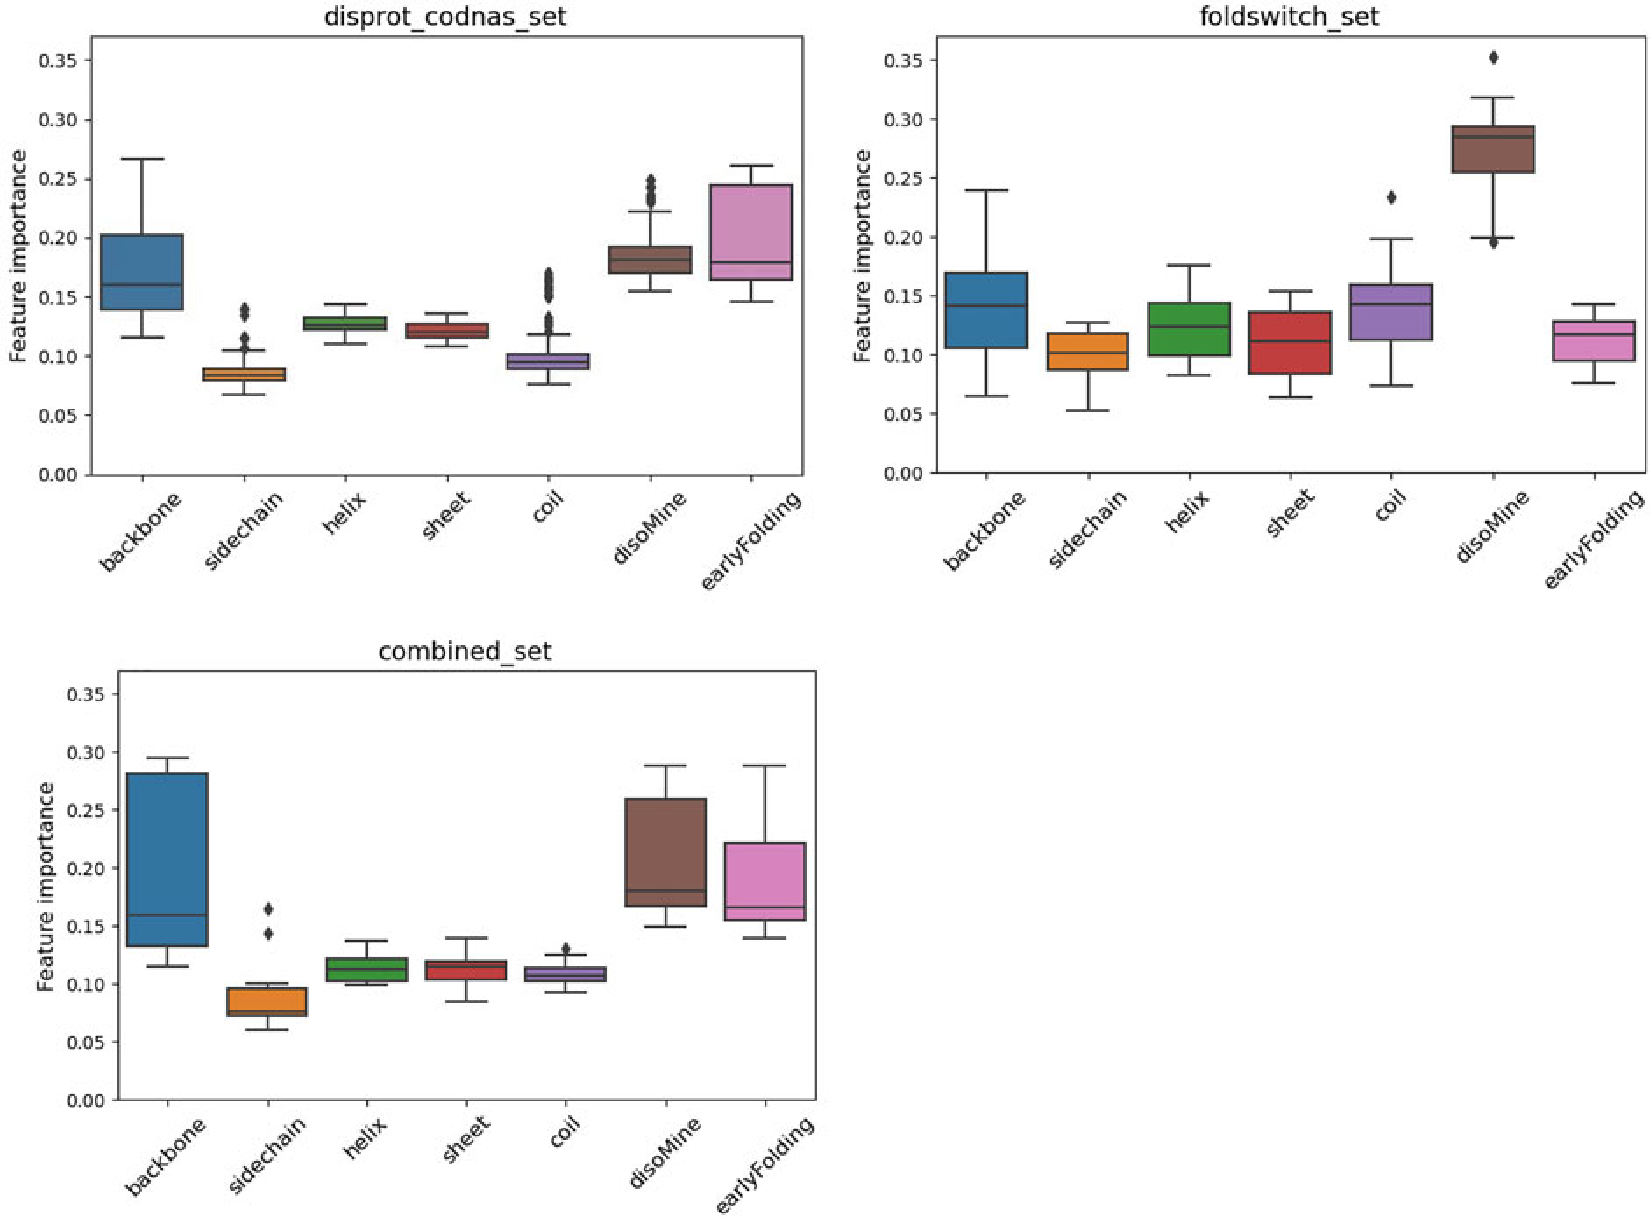
\includegraphics[width=\linewidth]{ambiguous//figures_ambiguous/fig2.pdf}
    \caption{\textbf{Feature importance variation for the RF classifier for the disprot_codnas_set (top left), the foldswitch_set (top right), and the combined_set (bottom left).}}
    \label{fig:chapter5:fig2}
\end{figure}

Finally, the \textbf{combined_RF} model where the O/S classes and the T/C classes were combined (\textbf{combined_set}) shows overall poorer F1 performances for the O/S classes compared to O and S separately, indicating that the definitions of O and S are likely different, while the T/C class F1 performance is in between the T and C classes, and the D performance drops (\tableref{tab:rf_performance}). The feature importance is similar to the one for the disprot_codnas_set (\figref{fig:chapter5:fig2}). Although there is an imbalance in the absolute numbers of the O compared to S, and T compared to C, classes, the sharp drop in overall performances indicates that the biophysical characteristics required for folding-upon-binding and for fold switching are fundamentally quite different.

The surrogate models generated from each of the RF models provide a perspective on the complexity of the data within. While both the codnas_disprot_set and combined_set surrogate models generate a large number of rules (84 and 89 rules, respectively), the surrogate model trained on the foldswitch_set is much simpler with just 11 rules, which makes it easier to interpret. We observed that the most disordered residues (DisoMine >= 0.897) are all predicted as transition (ambiguous behavior). Less disordered residues (DisoMine > 0.256) that present a low backbone rigidity (backbone <= 0.724 with DynaMine) are also classified as transition, as are residues with low backbone rigidity (backbone <= 0.754) and a high coil propensity (coil >= 0.505). The rest of the rules are often the combination of 3 or more biophysical features, disorder by DisoMine and backbone dynamics by DynaMine being the most prevalent ones, as already observed in the RF feature importance analysis (\figref{fig:chapter5:fig2}).


\subsection{Assessments on Independent MFIB Dataset}

To assess to what extent the RF predictor can recognize the conditional fold of IDPs undergoing mutual folding upon binding, we assembled a validation set based on the MFIB database \cite{ficho_mfib_2017} with structural filtering and removal of overlap with other training datasets (for details, see Methods). These proteins are quite different from the classical IDPs, as they are only disordered in absence of their binding partner or under conditions that prevent their homo-oligomerization, otherwise they fold into compact domain-like structures. Thus, we expected to see an enrichment of the predicted ordered and ambiguous conformational class as opposed to the enrichment of the disordered class.

\begin{figure}[tbh]
    \centering
    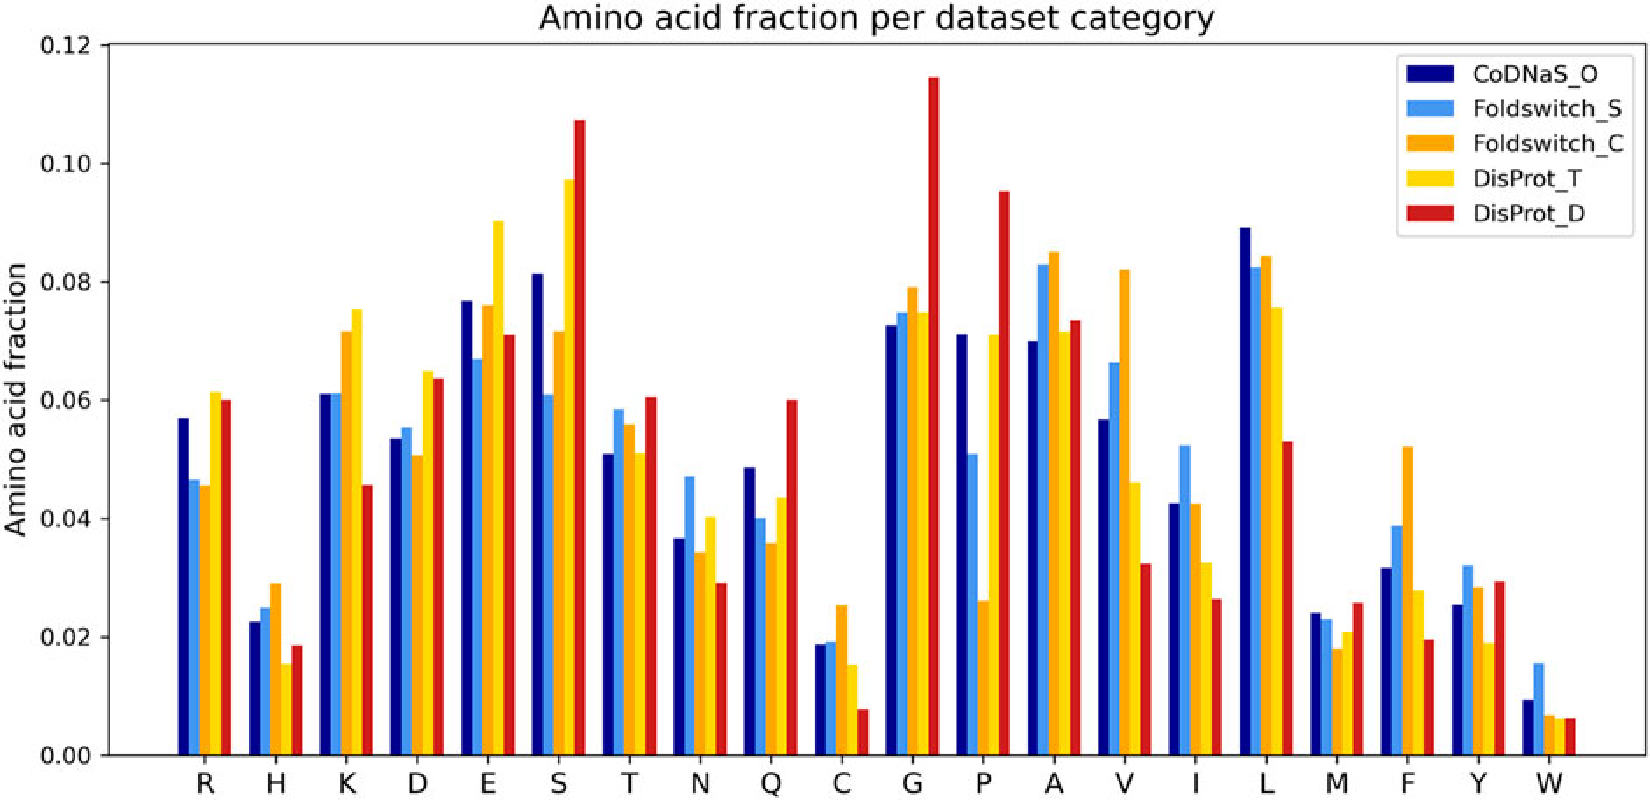
\includegraphics[width=\linewidth]{ambiguous//figures_ambiguous/fig3.pdf}
    \caption{\textbf{Amino acid fractions observed in the disprot_codnas_set for ordered residues (CoDNaS_O), transition (DisProt_T), and disordered (DisProt_D) and the foldswitch_set for fold-switching residues (Foldswitch_C) and residues that stay in the same fold (Foldswitch_S).}}
    \label{fig:chapter5:fig3}
\end{figure}

\begin{figure}[tbh]
    \centering
    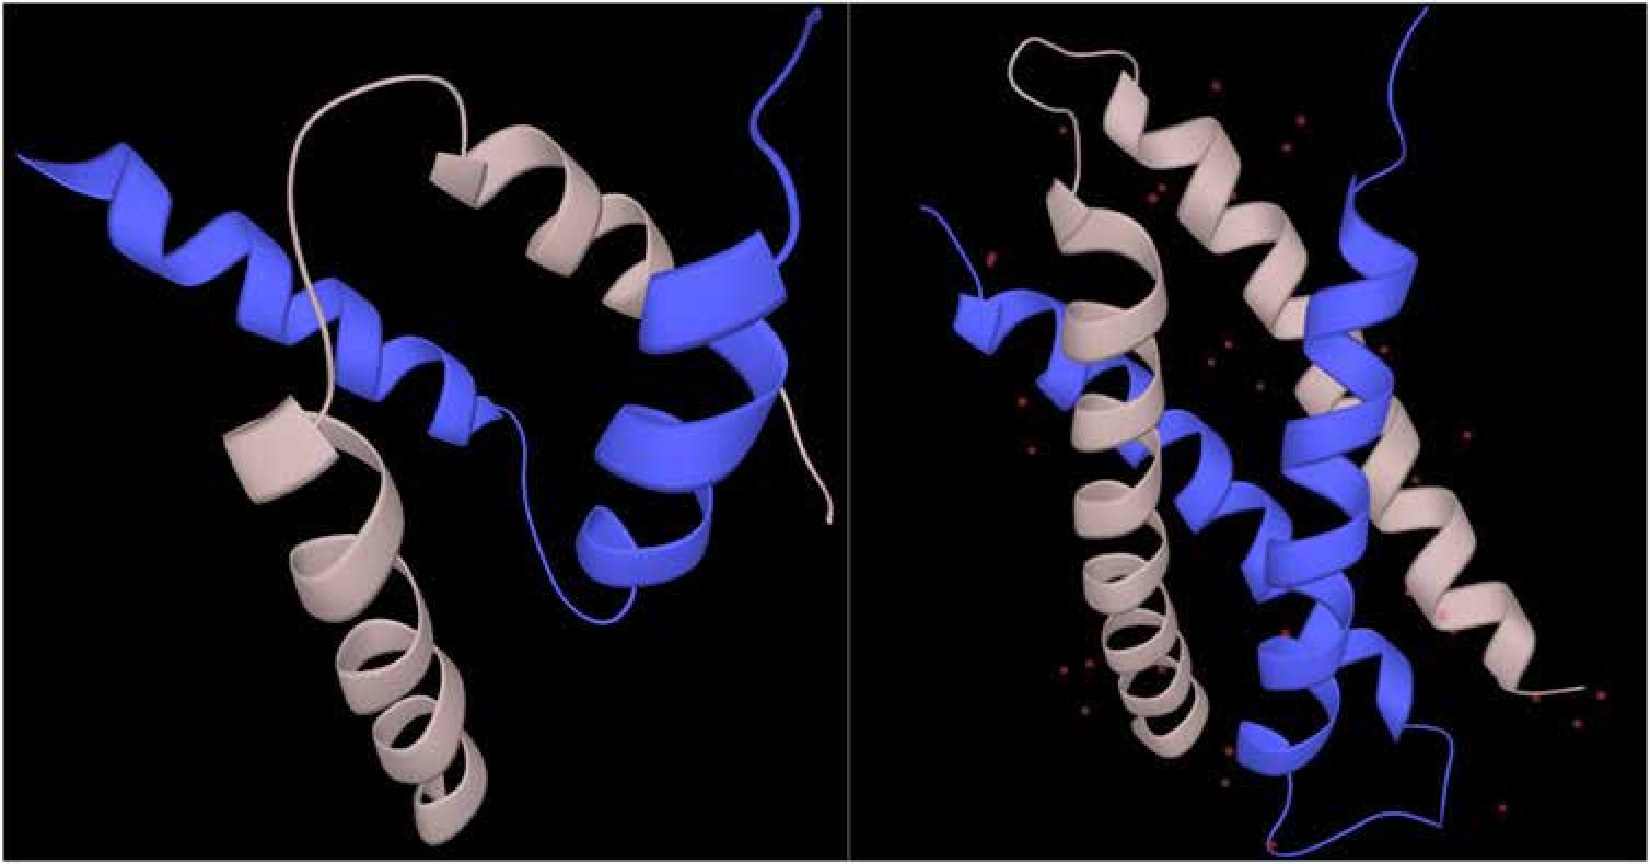
\includegraphics[width=\linewidth]{ambiguous//figures_ambiguous/fig4.pdf}
    \caption{\textbf{SinR and SH2B2 dimerization domains from MFIB (MF2120029, MF2100004).} The SinR (left) dimerization domain (PDB:2YAL) is predicted to have only ambiguous residues, while the SH2B2 (right) dimerization domain (PDB:1Q2H) is predicted to be fully ordered based on the combined_RF model.}
    \label{fig:chapter5:fig4}
\end{figure}

For the residues in regions undergoing synergistic folding, the disordered class, without ambiguous folding propensity, was shown to be depleted in the output of the combined_RF predictor (<1\%), while the ordered class was predicted to be the most represented (79.6\%). The ambiguous class was predicted for 20\% of cases, indicating that the folding mechanism of complexes in MFIB, in terms of biophysics, resembles folded domains. This resemblance of folded domains and mutually folded IDPs have already been recognized earlier from the structural and coevolution point of view \cite{iserte_chasing_2020}. A significant proportion of ambiguous behavior is still present, however, though fewer than disorder-to-order transitions of IDPs upon binding or to metamorphic fold-switchers. For individual cases, predictions of regions with ambiguous conformations had significant variation. For example, the SinR dimerization domain of B. subtilis [MFIB:MF2120029; PDB:2YAL] is predicted to have ambiguous conformation with 94\% coverage of the domain. On the other hand, the dimerization domain of the human SH2B adapter protein 2 [MFIB:MF2100004; PDB:1Q2H] is predicted to be 100\% ordered despite the structural resemblance to the other case (\figref{fig:chapter5:fig4}). The complete prediction file is available from \burl{https://bitbucket.org/bio2byte/protein_ambiguity/}.


\begin{figure}[tbh!]
    \centering
    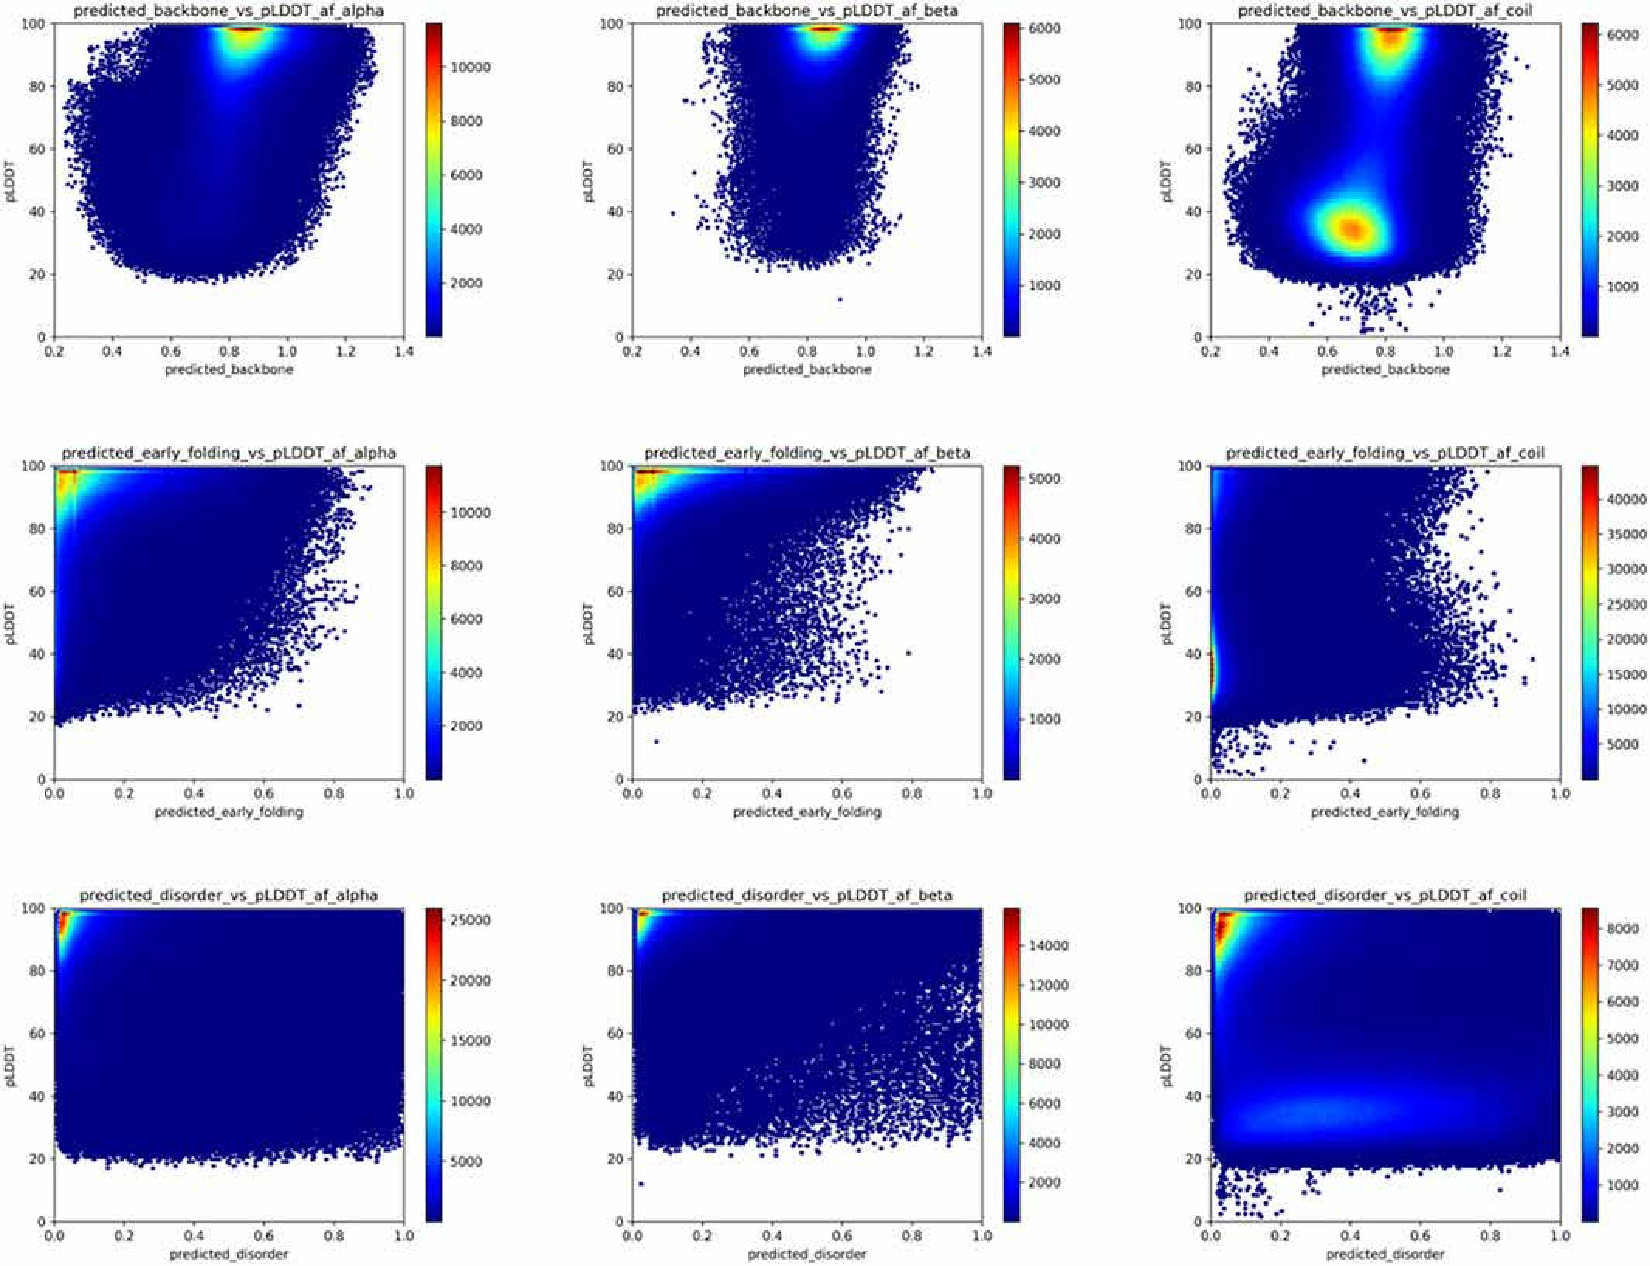
\includegraphics[width=\linewidth]{ambiguous//figures_ambiguous/fig5.pdf}
    \caption{\textbf{AlphaFold2 pLDDT versus backbone rigidity, early folding and disorder predictions for human proteome residues.} Based on the ``selected_human_dataset'', we show heat maps of the relation between AlphaFold2 pLDDT value and the backbone rigidity (top), early folding (middle), and disorder (bottom) predictions for residues designed at alpha-helix (left), beta-strand (middle) and coil (right) by DSSP based on the AlphaFold2 models.}
    \label{fig:chapter5:fig5}
\end{figure}

\subsection{Relation to AlphaFold2 Human Proteome Models}
AlphaFold2 \cite{jumper_highly_2021} can predict single low-energy conformations of proteins with unprecedented accuracy, and provides excellent indications of the confidence with which this is done through the per-residue pLDDT values. However, possible conformational ambiguity is not well captured by the AlphaFold2 models \cite{chakravarty_alphafold2_2022}, indicating the need to understand how the characteristics of these models relate to conformational ambiguity and dynamics. We therefore related the key biophysical predictions of the selected_human_set with the respective pLDDT values of AlphaFold2 models, subdivided by secondary structure category in the model as determined by DSSP, to understand how these are related, and how this can give insights in the ambiguous residue categories. \figref{fig:chapter5:fig5} shows that for the backbone dynamics predictions (first row) the confidently predicted alpha-helix or beta-strand residues, with pLDDT scores close to 100\%, have high predicted rigidity (>0.8 DynaMine score); for DynaMine, residues with values above 0.8 are expected to be well folded \cite{cilia_dynamine_2014}. Residues with a coil classification according to DSSP are either similar to the secondary structure categories (pLDDT confident/ backbone rigid), indicating folded residues that do not fall into regular secondary structure categories, or they have low pLDDT confidence and are in the ``context-dependent'' (DynaMine scores between 0.69 and 0.80), or in the flexible region (<0.69). The pLDDT and DynaMine scores are therefore aligned, with high backbone dynamics (lower DynaMine scores) indicating multiple conformations correlating with AlphaFold2 predictions of lower confidence, as it is not able to confidently predict a single low-energy conformation for these residues. The early folding propensity predictions (\figref{fig:chapter5:fig5}, second row), show that residues with increased early folding propensity are also typically residues predicted with high confidence by AlphaFold2, although AlphaFold2 cannot distinguish between these residues and ones that do not initiate folding pathways, as already indicated by other studies \cite{outeiral_current_2022}. Finally, for disorder predictions (\figref{fig:chapter5:fig5}, third row), regions with high pLDDT are enriched with residues predicted to have disorder scores of 0 (no disorder), whereas residues predicted to be coil by AlphaFold2 features a low pLDDT region that has a wide dispersion of datapoints covering a range of disorder propensity values. Similar to backbone dynamics, this indicates residues that might have ambiguous conformational behavior.

\begin{figure}[tbh]
    \centering
    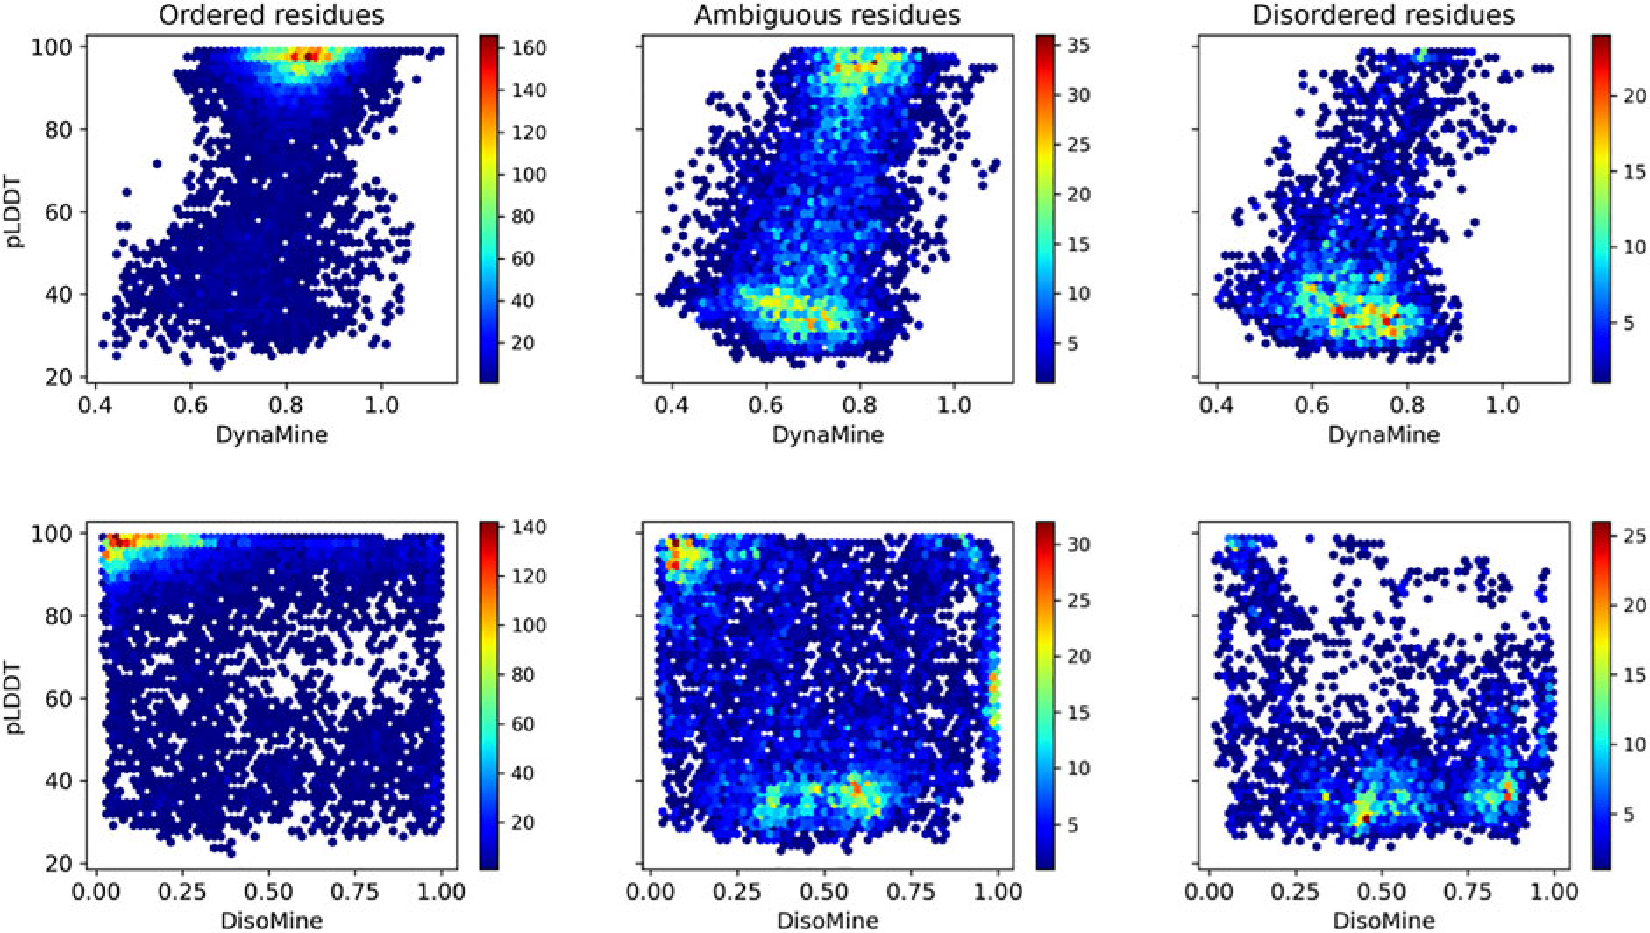
\includegraphics[width=\linewidth]{ambiguous//figures_ambiguous/fig6.pdf}
    \caption{\textbf{Relation between pLDDT score and backbone dynamics (top) and disorder (bottom) for the O/T/D classes from the disprot_codnas_set}}
    \label{fig:chapter5:fig6}
\end{figure}

When subdividing these plots in relation to our datasets that indicate ambiguous residues (\figref{fig:chapter5:fig6}), these trends are more obvious. The ordered residues cluster at high pLDDT values (>80\%) and high backbone rigidity (>0.8), the disordered residues at very low pLDDT values (<40\%) and high backbone dynamics (<0.8). The ambiguous residues fall in between these categories, with many lower confidence pLDDT values between 80\% and 40\%, and backbone dynamics between 0.70-0.80, as well as significant overlap with the ordered and disordered categories. The disorder values confirm this trend, with few ordered residues predicted as having high disorder scores, and most disordered residues correctly predicted with high disorder scores. The ambiguous residues again give an intermediate picture, with more residues having scores intermediate between the typical scores for order and disorder.

For the \textbf{fold_switch_set} only (\figref{fig:chapter5:fig7}), there are interesting differences in especially the AlphaFold2 pLDDT scores, which tend to be below 90\% for the residues that change conformation. The backbone dynamics also contains fewer high values, while more residues are predicted with high disorder.


\subsection{Relation to Post-Translational Modification Data}

Post-translational modifications (PTMs) of amino acid residues are important for regulation and can have a significant impact on protein conformation and function. Based on the \textbf{ptm_set}, which contains information for sumoylation, methylation, acetylation, ubiquitination and phosphorylation, or a combination of these (\figref{fig:chapter5:fig8}, log scale), we subdivided the observed PTMs by the different datasets. For the \textbf{disprot_codnas_set}, the majority of PTMs are observed in the Order and Transition classes, with phosphorylation overrepresented in residues with transition properties, and with ubiquitination and sumoylation underrepresented (\figref{fig:chapter5:fig8} B). In the \textbf{foldswitch_set}, residues that remain in the Same secondary structure state (S) have again increased ubiquitination and sumoylation compared to residues that Convert (C), with a slight increase for acetylation and especially multiple modifications, indicating a possible role in fold-switching processes, or more availability of these residues to be modified by smaller PTMs. The trends for the \textbf{combined_set} are very similar to the \textbf{disprot_codnas_set}, which constitutes the bulk of the data.

\begin{figure}[tbh]
    \centering
    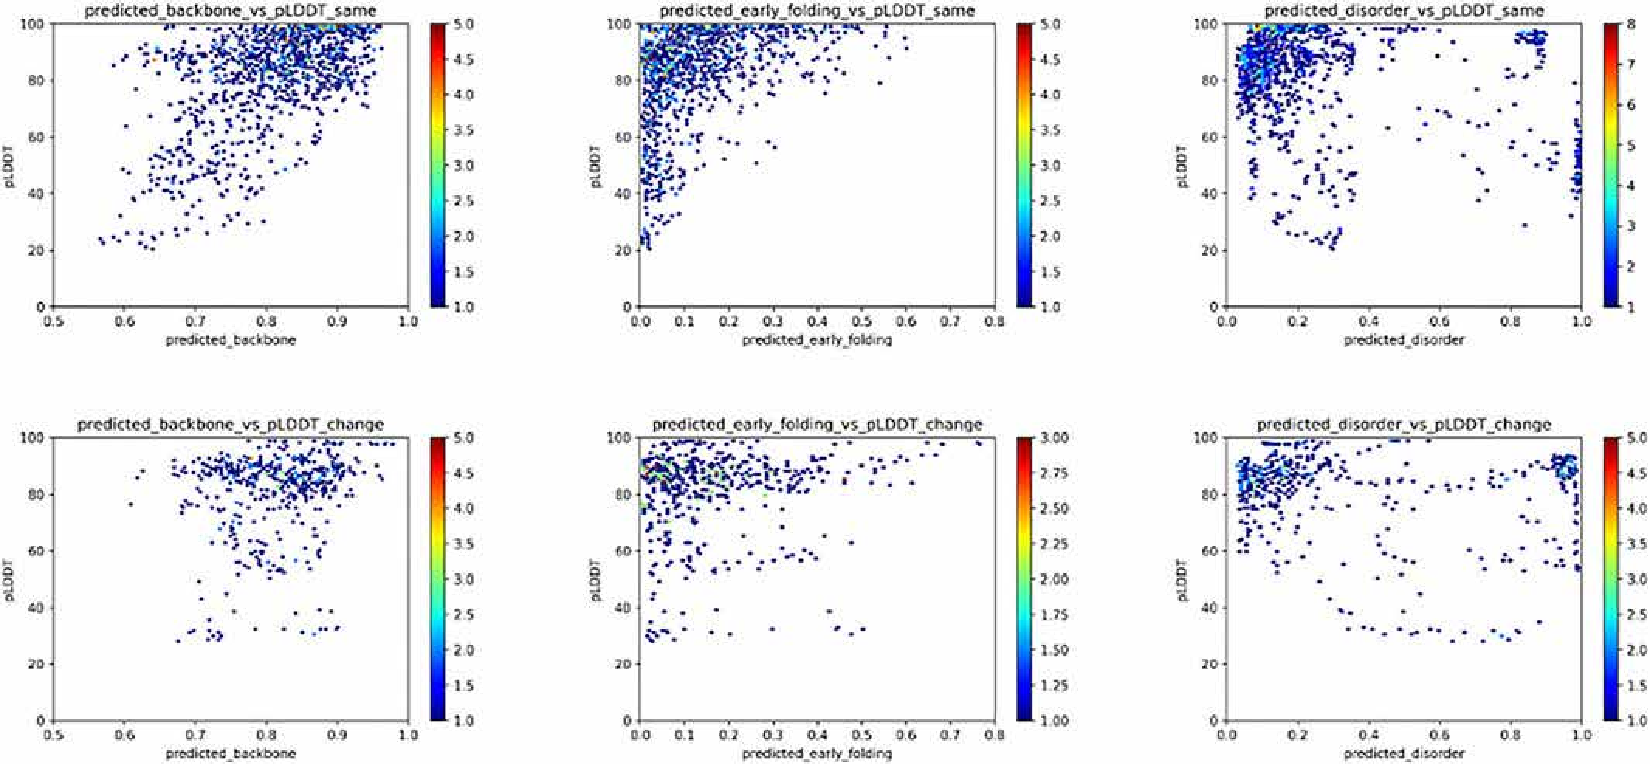
\includegraphics[width=\linewidth]{ambiguous//figures_ambiguous/fig7.pdf}
    \caption{\textbf{Relation between the pLDDT score and backbone dynamics (left), early folding (middle), disorder (right) for the fold_switch_set same (top row), and convert (bottom row) residues.}}
    \label{fig:chapter5:fig7}
\end{figure}

\begin{figure}[tbh]
    \centering
    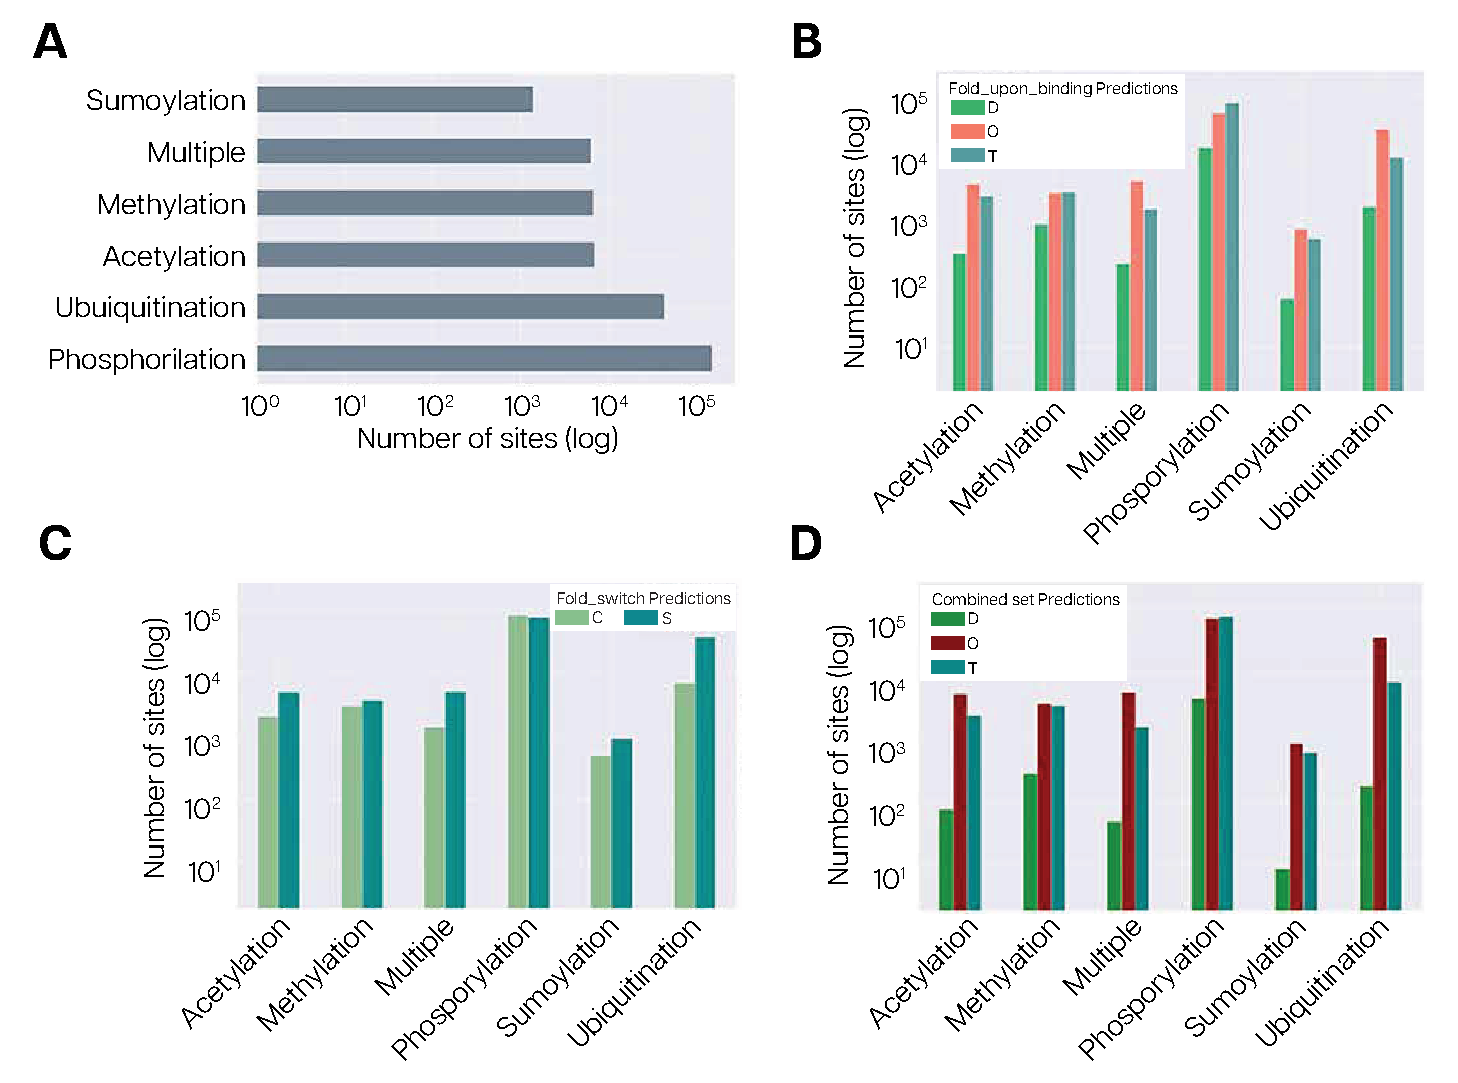
\includegraphics[width=\linewidth]{ambiguous//figures_ambiguous/fig8_corrected.pdf}
    \caption{\textbf{Post-translational modification (PTM) sites from the ptm_set in relation to datasets.} The total number of included PTMs (A), subdivided by disordered, ordered, and transition based on disprot_codnas_set (B), by ordered and convert based on foldswitch_set (C), and based on the combined order, disorder, and transition classes (D).}
    \label{fig:chapter5:fig8}
\end{figure}

\begin{figure}[tbh]
    \centering
    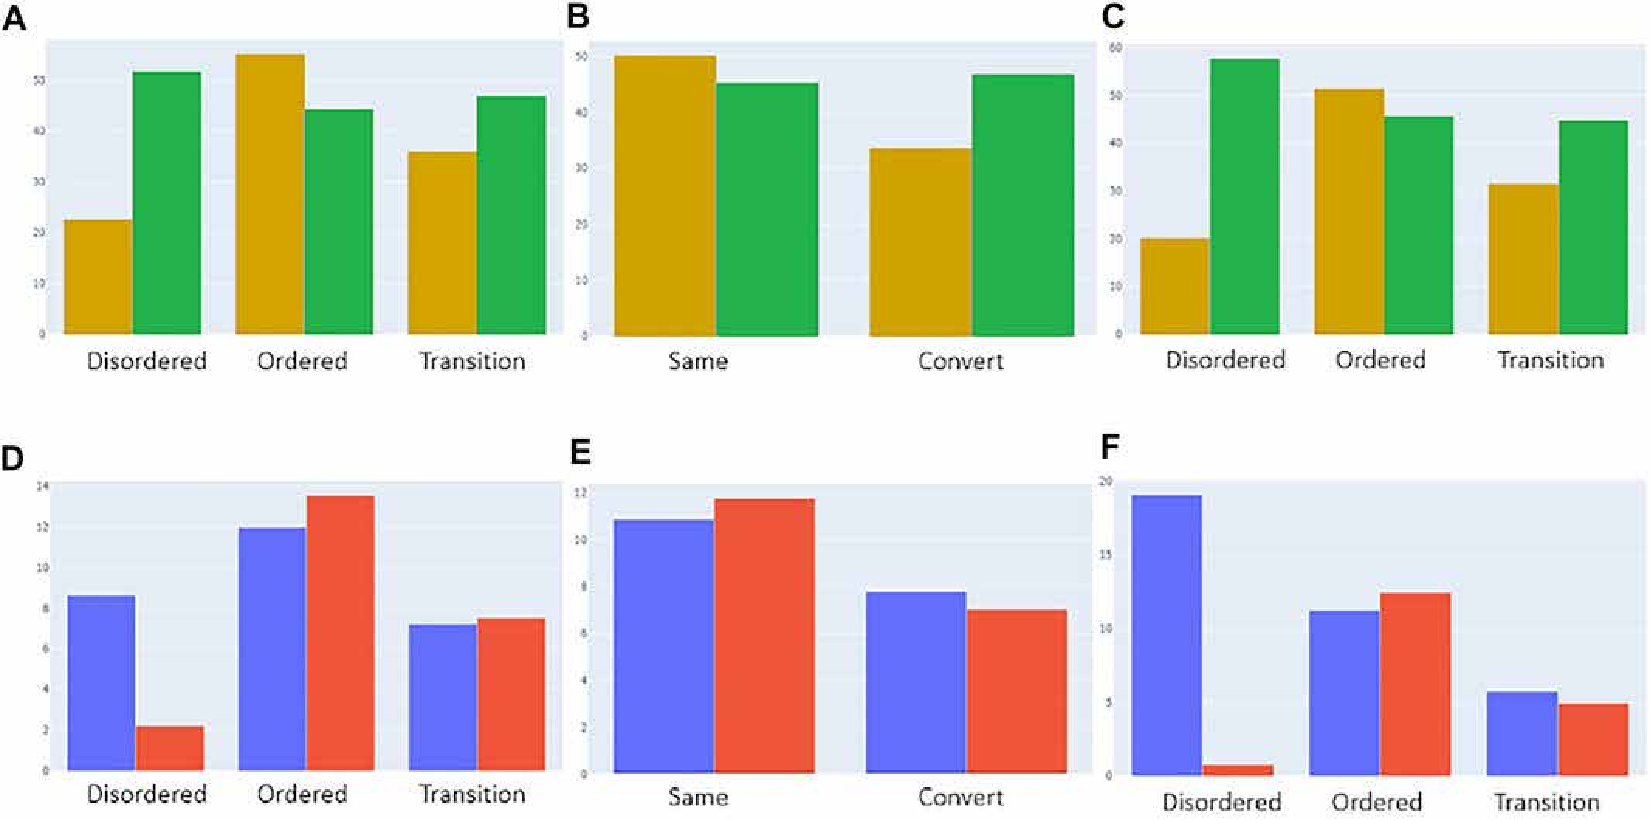
\includegraphics[width=\linewidth]{ambiguous//figures_ambiguous/fig9.pdf}
    \caption{\textbf{Categorization of deleterious (yellow) and benign (green) mutations from the “canonical_mut” dataset classified as disordered, ordered, and ambiguous based on models 1 [(A), top left], 2 [(B), top middle], and 3 [(C), top right], respectively.} The distributions were normalized by the total number of assigned ordered, disordered and ambiguous residues in the dataset. Categorization of germline (blue) and somatic (red) mutations from the “germline_somatic_deleterious” dataset classified as disordered, ordered, and ambiguous based on models 1 [(D), bottom left], 2 [(E), bottom middle], and 3 [(F), bottom right], respectively. The distributions were normalized by the total number of assigned ordered, disordered and ambiguous residues in the dataset and the number of somatic/germline ratios for better comparison.}
    \label{fig:chapter5:fig9}
\end{figure}

\subsection{Relation to Deleterious Amino Acid Variants}
We also investigated whether residues in ambiguous regions, again given their likely role in conformational rearrangements and allostery, are more likely to contain deleterious or benign mutations, as classified in the canonical_mut dataset. \figref{fig:chapter5:fig9}A shows that for the \textbf{disprot_codnas_set} (RF model 1), the ordered residues contain, as expected, relatively more deleterious mutations. Although the ambiguous residues contain more benign mutations, they still contain a high proportion of deleterious mutations, especially compared to the ratio observed for disordered residues. This situation is similar for somatic versus germline cancer mutations (\figref{fig:chapter5:fig9} D). For the \textbf{foldswitch_set} (RF model 2), the ambiguous metamorphic residues contain a higher amount of deleterious mutations than the residues that retain their secondary structure (\figref{fig:chapter5:fig9} B), whereas there is no difference for somatic versus germline mutations (\figref{fig:chapter5:fig9} E). For the combined RF model 3, the trends are very similar to RF model 1 (\figref{fig:chapter5:fig9} C/F).


\section{Discussion}

In this exploratory analysis, we use two datasets that try to capture amino acid residues in proteins that display different ``ambiguous'' behavior, either by folding upon binding (\textbf{disprot_codnas_set}), or by changing secondary structure in metamorphic proteins (\textbf{foldswitch_set}). This definition of ``ambiguous'' residues is highly relevant given the ready availability of predicted AlphaFold2 protein structure models with qualities comparable to experimentally derived structures. Given the dynamic nature of proteins, and their capacity to change conformation and transmit signals through allostery \cite{tompa_multisteric_2014, tompa_principle_2016}, annotations of the AlphaFold2 models that indicate where such conformational changes are more likely to happen will help in interpreting such models. Our results indicate that AlphaFold2, based on the per-residue pLDDT prediction confidence values, captures ordered and disordered residues very well, and while for ambiguous regions intermediate pLDDT values are observed, many of these ambiguous residues fall in the ``traditional'' ordered or disordered regions (\figref{fig:chapter5:fig6}). The RF models we created, and their interpretation, shows that sequence-predicted disorder is the most important factor predicting fold switching residues (from order to order), as well as folding-upon-binding (from disorder to order), with backbone dynamics and early folding also important for the last category. Specific amino acids are also a likely factor, such as valine and phenylalanine for the fold switching residues. Although the recognition by the combined_RF model of the MFIB dataset, which contains dimers that form domain-like structures, is of limited sensitivity (see \burl{https://bitbucket.org/bio2byte/protein_ambiguity/}), there are indications that ambiguous residues can also be picked up in these cases. This illustrates the complexity of protein behavior in relation to its (local) environment; in this case, and expressed in terms of ambiguous behavior, the local sequence context of the protein is strongly geared towards order, but enough ambiguous residues are present that the individual proteins cannot fold.

Previous AlphaFold2-related studies in this area have given similar indications. AlphaFold2 is a good predictor of intrinsically disordered regions (IDRs) based on the CAID PDB-DisProt dataset \cite{piovesan_intrinsic_2022}, a study on conditionally folded IDRs \cite{alderson_systematic_2022} showed that many IDR regions are in the high (70 $\leq$ x < 90) or very high ($\geq$ 90) pLDDT regions, similar to what we report, with an enrichment in helical conformations, and with long, extended single $\alpha$-helix domains not stabilized by tertiary contacts identified. For a subset of IDRs that fold under specific conditions and have been extensively characterized by NMR spectroscopy, the IDRs resemble the conformation of the folded state, even if there is no stable secondary structure observed with only a fractional preference to populate secondary structure from the experimental NMR data. The combination of higher relative solvent accessibility in the AlphaFold2 models, which indicates lack of overall structure, and high pLDDT scores, which indicate confident structure predictions, does however seem to be a good indicator of regions with a tendency for ambiguous behavior \cite{piovesan_intrinsic_2022}. These results show again that AlphaFold2 is excellent at defining a single low energy state for a given protein sequence, if it exists, but that the context of the protein and possible ambiguous behavior is more difficult to capture. Indeed, in relation to conformational diversity as observed in the PDB from \gls{apostate}-\gls{holostate} pairs of conformers for the same protein \cite{saldano_impact_2022}, AlphaFold2 predicts the holo form in ~70\% of cases, but is unable to capture both states. As the conformational diversity between the apo/holo states increases, its prediction performance also worsens. A similar picture is observed for proteins that can switch folds \cite{chakravarty_alphafold2_2022}, with 94\% of AlphaFold2 predictions capturing one experimentally determined conformation, but not the other, and with moderate-to-high pLDTT scores for 74\% of fold-switching residues, similar to our study. Finally, although AlphaFold2 and RoseTTAfold models seem to carry overall foldability information \cite{liu_computational_2022}, the folding process itself is not well captured \cite{outeiral_current_2022}, if at all.

Overall, it remains very difficult to capture dynamics properties of proteins; despite the availability of molecular dynamics simulations of increasing length, limited direct dynamics measurements from NMR and other structural biology approaches, and the observed conformational diversity in the PDB, the complexity of possible protein movements and their likelihood within the in vivo environment of proteins in general precludes the generation of relevant all-encompassing datasets. The increasing amount of data that indirectly indicates such behavior, from mass spectrometry proteomics \cite{britt_integration_2022} as well as from evolutionary and disease mutation sources, will be in this respect invaluable, as already indicated in our limited study. The challenge here lies in interconnecting the various diverse data sources, and analyzing the resulting complex information, which is beyond direct human understanding and requires machine learning approaches, preferably interpretable so that concepts and first principles can be derived from them. Further methodology development in the more traditional sense is also key, for example improved ensemble representations of proteins and especially IDRs, as already indicated in other studies such as the ones discussed here \cite{alderson_systematic_2022, chakravarty_alphafold2_2022}, as well as more accurate sequence-based predictors, with the combination of structure and sequence-based approaches likely giving the most relevant results.

\section{Conclusion}
In our view, it is essential that we move away from the two-state view of proteins (one single well defined static fold, or complete disorder) to a more nuanced probabilistic view, where the ``probability space'' of proteins is defined – the possible states a protein can adopt. The definition of the different kinds of ambiguity observed in protein behavior, and their interpretation, is an important step to help the field move in this direction. Ongoing ELIXIR implementation projects, for example, are also focusing on related topics, highlighting the community need for this kind of probabilistic interpretation of protein behavior.  We hope that the datasets and analyses we assembled here provide additional reference points to further explore and define residues with ambiguous behavior in proteins.

% \section*{Conflict of Interest}
% The authors declare that the research was conducted in the absence of any commercial or financial relationships that could be construed as a potential conflict of interest.

% \section*{Funding}
% European Union’s Horizon 2020 research and innovation programme under the Marie Skłodowska-Curie grant agreement [813239 to J.R.-M. and J.G.-G.]; Research Foundation Flanders (FWO) [G.032816N to B.D., G.028821N to D.B.]; Vrije Universiteit Brussel Research Council under the Interdisciplinary Research Program TumorScope [IRP20 to K.T.]; Tempus Public Foundation postdoctoral fellowships [158534 and 166538 to R.P.]; National Research, Development and Innovation Office research grant [FK128133 to R.P.]. Funding for open access charge: European Union’s Horizon 2020 research and innovation programme under the Marie Skłodowska-Curie grant agreement [813239].

\section*{Data availability}
The datasets generated and analysed for this study can be found in \burl{https://bitbucket.org/bio2byte/protein_ambiguity/}.


\subfile{pLDDT/main_plddt}

\subfile{b2b_deployment/main_b2b_deployment}



% Non-first papers

% \chapter{Online biophysical predictions for SARS-CoV-2 proteins.}\label{chapter:corona}
\chaptermark{Biophysical predictions for SARS-CoV-2}

Luciano Kagami $^{1}$, Joel Roca-Martinez $^{1,2,3}$, Jose Gavalda-Garcia $^{1,2}$, Pathmanaban Ramasamy $^{1,2,3,4,5}$, K. Anton Feenstra $^{6,7}$, and Wim Vranken $^{1,2,3}$
\\
\\
$^{1}$ Interuniversity Institute of Bioinformatics in Brussels, ULB-VUB, \\Brussels, Belgium.
\\
$^{2}$ Structural Biology Brussels, Vrije Universiteit Brussel, Brussels, Belgium.
\\
$^{3}$ VIB Structural Biology Research Centre, Pleinlaan 2, 1050 Brussels, Belgium.
\\
$^{4}$ VIB-UGent Center for Medical Biotechnology, VIB, 9000 Ghent, Belgium.
\\
$^{5}$ Department of Biomolecular Medicine, Faculty of Health Sciences and Medicine, Ghent University, 9000 Ghent, Belgium.
\\
$^{6}$ IBIVU – Center for Integrative Bioinformatics, Department of Computer Science, Vrije Universiteit Amsterdam, Amsterdam, 1081HV The Netherlands.
\\
$^{7}$ AIMMS – Amsterdam Institute for Molecules Medicines and Systems, Vrije Universiteit Amsterdam, Amsterdam, 1081HV The Netherlands.
\\
\\
DOI: 10.1186/s12860-021-00362-w
\vspace{1em}
\hrule
\vspace{1em}

\begin{abstract}
    \textbf{Background:} The SARS-CoV-2 virus, the causative agent of COVID-19, consists of an assembly of proteins that determine its infectious and immunological behavior, as well as its response to therapeutics. Major structural biology efforts on these proteins have already provided essential insights into the mode of action of the virus, as well as avenues for structure-based drug design. However, not all of the SARS-CoV-2 proteins, or regions thereof, have a well-defined three-dimensional structure, and as such might exhibit ambiguous, dynamic behaviour that is not evident from static structure representations, nor from molecular dynamics simulations using these structures.

    \textbf{Main:} We present a website (\burl{https://bio2byte.be/sars2/}) that provides protein sequence-based predictions of the backbone and side-chain dynamics and conformational propensities of these proteins, as well as derived early folding, disorder, $\beta$-sheet aggregation, protein-protein interaction and epitope propensities. These predictions attempt to capture the inherent biophysical propensities encoded in the sequence, rather than context-dependent behaviour such as the final folded state. In addition, we provide the biophysical variation that is observed in homologous proteins, which gives an indication of the limits of their functionally relevant biophysical behaviour.

    \textbf{Conclusion:} The \burl{https://bio2byte.be/sars2/} website provides a range of protein sequence-based predictions for 27 SARS-CoV-2 proteins, enabling researchers to form hypotheses about their possible functional modes of action.
\end{abstract}
% \chapter{b2bTools: online predictions for protein biophysical features and their conservation.}\label{chapter:b2b_online}
\chaptermark{b2BTools online predictions}

Luciano Porto Kagami $^{1}$, Gabriele Orlando $^{1}$, Daniele Raimondi $^{1}$, François Ancien $^{1,2}$, Bhawna Dixit $^{1,2,3}$, Jose Gavalda-Garcia $^{1,2,3}$, Pathmanaban Ramasamy $^{1,4,5,6}$, Joel Roca-Martinez $^{1,3,4}$, Konstantina Tzavella $^{1,3,4}$, and Wim Vranken $^{1,3,4}$
\\
\\
$^{1}$ Interuniversity Institute of Bioinformatics in Brussels, ULB-VUB, \\Brussels, Belgium.
\\
$^{2}$ 3Bio, Université Libre de Bruxelles, Brussels 1050, Belgium.
\\
$^{3}$ Structural Biology Brussels, Vrije Universiteit Brussel, Brussels, Belgium.
\\
$^{4}$ Structural Biology Research Centre, Pleinlaan 2, 1050 Brussels, Belgium.
\\
$^{5}$ VIB-UGent Center for Medical Biotechnology, VIB, 9000 Ghent, Belgium.
\\
$^{5}$ Department of Biomolecular Medicine, Faculty of Health Sciences and Medicine, Ghent University, 9000 Ghent, Belgium.
\\
\\
DOI: 10.1093/nar/gkab425.

\vspace{1em}
\hrule
\vspace{1em}

\begin{abstract}
    We provide integrated protein sequence-based predictions via \burl{https://bio2byte.be/b2btools/}. The aim of our predictions is to identify the biophysical behaviour or features of proteins that are not readily captured by structural biology and/or molecular dynamics approaches. Upload of a FASTA file or text input of a sequence provides integrated predictions from DynaMine backbone and side-chain dynamics, conformational propensities, and derived EFoldMine early folding, DisoMine disorder, and Agmata $\beta$-sheet aggregation. These predictions, several of which were previously not available online, capture 'emergent' properties of proteins, i.e. the inherent biophysical propensities encoded in their sequence, rather than context-dependent behaviour (e.g. final folded state). In addition, upload of a multiple sequence alignment (MSA) in a variety of formats enables exploration of the biophysical variation observed in homologous proteins. The associated plots indicate the biophysical limits of functionally relevant protein behaviour, with unusual residues flagged by a Gaussian mixture model analysis. The prediction results are available as JSON or CSV files and directly accessible via an API. Online visualisation is available as interactive plots, with brief explanations and tutorial pages included. The server and API employ an email-free token-based system that can be used to anonymously access previously generated results.
\end{abstract}



\chapter{Discussion}
\newpage

This thesis has focused on describing protein conformation as a dynamic property under physiological conditions. Such a description is challenging, and diverse strategies can be employed to study it from different perspectives. Nuclear Magnetic Resonance spectroscopy (NMR) experiments can be employed to measure biophysical properties such as order ($S^{2}$) and flexibility (Random Coil Index), describing backbone and side chain dynamics. Another NMR approach to describe a protein's dynamic conformation is the elucidation of structural ensembles at physiological temperatures. Computationally, Molecular Dynamics (MD) simulations also produce protein structural ensembles, with the particularity that they are presented in a time-series. Both approaches, the coordinate-free measurement of biophysical properties and the elucidation of structural ensembles, have been considered in this thesis. 

\section{Conformational State Propensities and Variability}
\sectionmark{Conf. State Propensities and Variability}

A recurrent theme throughout this work is that protein conformation is better described as an ensemble of structures representing the possible conformations that a protein can adopt and transition among in physiological conditions. Beyond the visualisation of all structures and alignment-derived metrics (\textit{e.g.} RMSD), extracting meaningful information from these ensembles can be challenging. Though these atomic precision structures are key to describing protein conformation, their sole usage to describe a protein's conformational landscape is unlikely to cover all possible conformations. Considering, as an example, a protein with 5 loci, each with 5 possible defined conformations (and assuming they are distant enough not to influence each other), the calculation of all possible protein conformation is subject to combinatorial explosion of $5^{5}=3125$ possible conformations. This highlights the need for new metrics for describing conformational diversity.

In this context, Constava (chapter \ref{chapter:constava}) \cite{gavalda-garcia_data-driven_2024} offers a method capable of leveraging information from these ensembles to produce novel residue-level descriptions of protein conformation. This description can also be applied to interpret structural ensembles in changing or differential conditions, providing additional metrics to perform such a challenging analysis.

\subsection{Probabilistic Definition of Conformational States and its Relation to Free Energy Landscapes}

Six conformational states are probabilistically defined within the backbone dihedral space, representing different dynamic states of traditional secondary structures. Although more conformational states could describe additional unique local conformations, we limited our definition to these six states to ensure that each state was represented by a sufficient number of data points. The data used to fit each of the six Probability Density Functions (PDFs) were selected based on criteria from NMR structural ensembles and interpreted chemical shifts (\figref{overal_figure}) \cite{orlando_shiftcrypt_2020}. 

The NMR-derived definition of these conformational states should therefore make them more suitable to describe protein local conformation in physiological temperatures than crystallography-benchmarked secondary structures. \textcolor{red}{Defining these conformational states using solution NMR data implicitly incorporates the effects of water, so better reflecting the biological environment of proteins and including more conformational states than those typically observed in crystallography}. Specifically, the introduction of the ``Surrounding Helix'' and ``Surrounding Sheet'' conformational states incorporates the concepts of relaxed local conformations, which behave somewhat like an $\alpha$-helix or $\beta$-sheet/strand, but show higher dynamism than their ``Core'' forms. The latter, ``Core'' conformational states, indicate closer resemblance to traditional definitions of $\alpha$-helix or $\beta$-sheet/strand, even at physiological temperatures. 

This distinction accommodates for hybrid behaviours between order and disorder found at physiological temperatures. In contrast, the cryogenic temperatures required for X-ray crystallography and Cryogenic Electron Microscopy (Cryo-EM) facilitate the acquisition of local conformation by reducing the Gibbs free energy in the system. This stabilises proteins into their native conformation, at energy levels that prevent transition to other conformations which are available at physiological temperatures. The separation between ``Core'' and ``Surrounding'' conformational states represent residues that most likely would be assigned to the same secondary structure at cryogenic temperatures (\figref{fig:discussion:surrhelix_vs_xray}), now distinguished in two states. 

\begin{figure}[htb!]
    \centering
    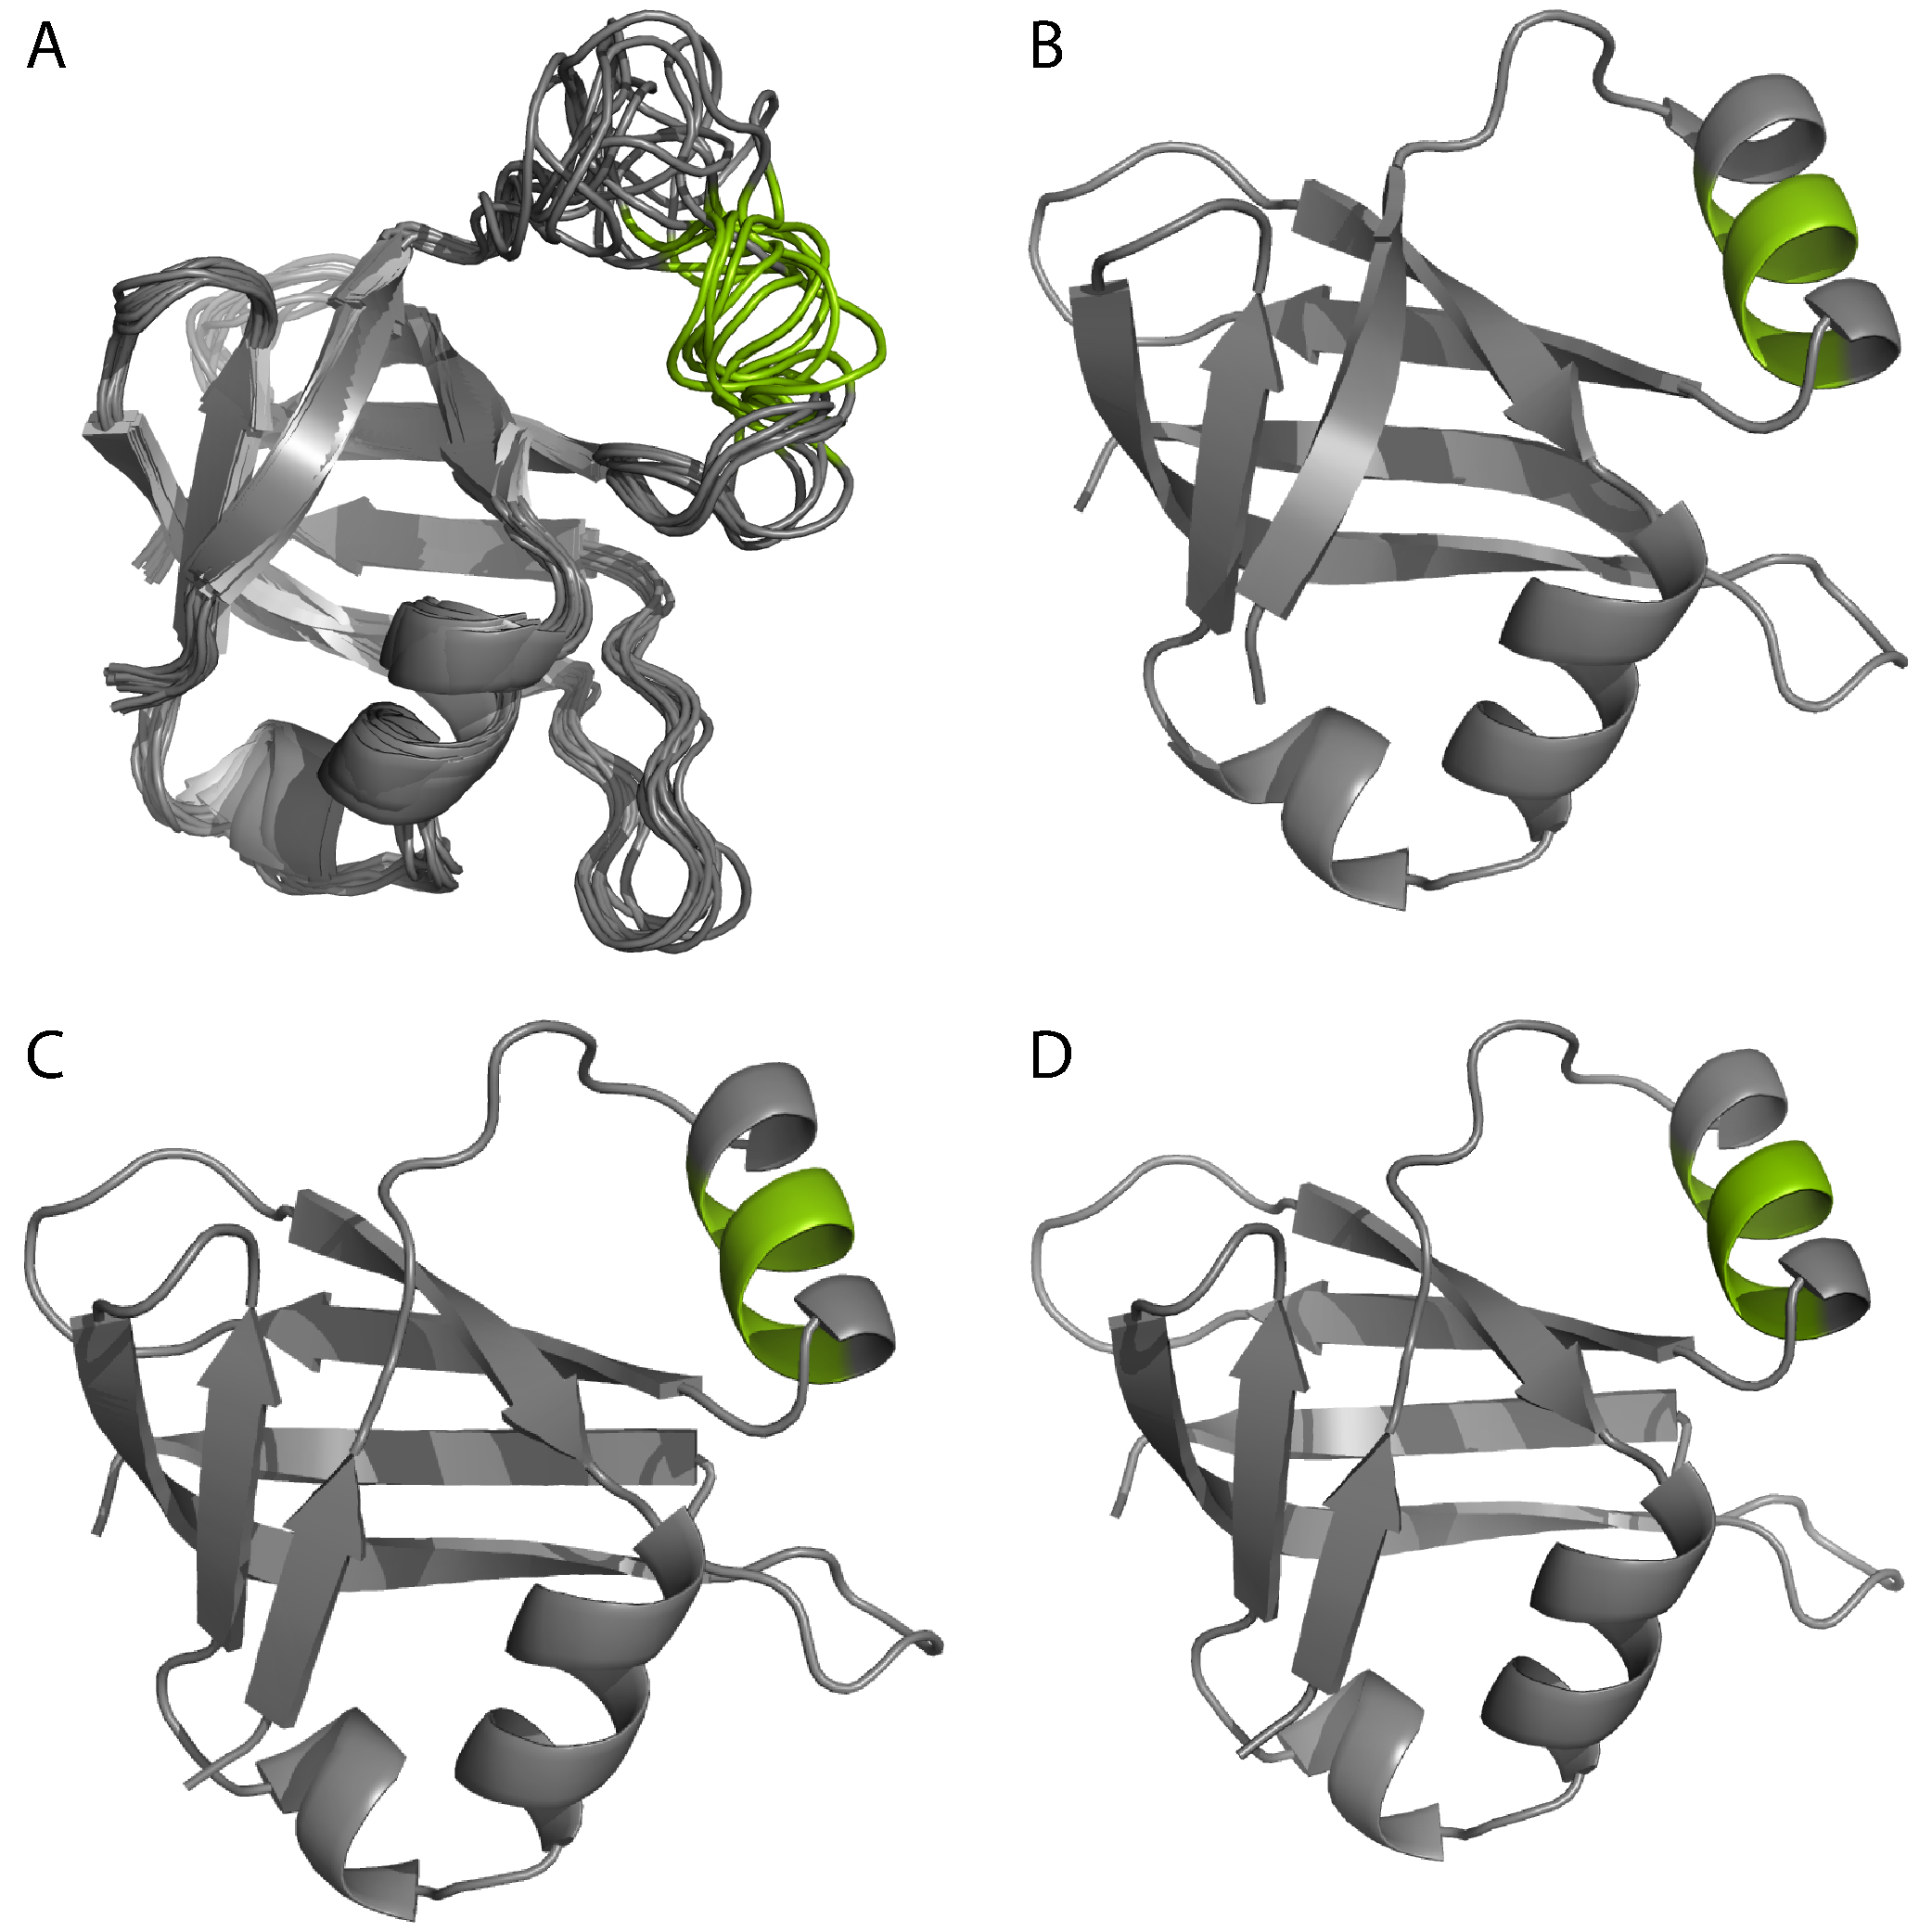
\includegraphics[width=0.85\linewidth]{figures/surrounding_notin_cryo.pdf}
    \caption{\textbf{Surrounding helix stabilisation into defined $\alpha$-helix by cryogenic temperatures in Cryo-EM in \textit{E. coli} ribosomal protein L25.} A) NMR ensemble (PDB id: 1B75 \cite{stoldt_nmr_1998}), with highlighted region indicating region with mixed ``Surrounding helix'' and ``Core helix'' for Constava's window sampling sizes 3 and 25, calculated on the corresponding MD simulation in \cite{gavalda-garcia_data-driven_2024} (dataframes in \burl{https://doi.org/10.5281/zenodo.10371447}) 
    B) Cryo-EM structure (PDB id: 8CGK \cite{paternoga_structural_2023}, chain W) with the same highlighted region adopting a canonical $\alpha$-helix conformation. 
    C) AlphaFold2 model of the protein (\burl{https://alphafold.ebi.ac.uk/entry/P68919}). The highlighted region is canonically folded, as in Cryo-EM. 
    D) AlphaFold3 model of the protein (calculated on \burl{https://alphafoldserver.com/} with sequence from UniProt id: P68919). The highlighted region is also canonically folded, as in Cryo-EM. 
    }
    \label{fig:discussion:surrhelix_vs_xray}
\end{figure}

The PDFs defining each conformational state are inversely related to their free energy landscape, where higher densities on a PDF denote thermodynamically favourable energy minima. If each conformational state is viewed as a local conformation macro-state, the state's likelihood maxima (or energy minima) in each PDF describe local conformation micro-states. ``Core'' conformational states, especially the ``Core helix'', exhibit very few micro-states within the macro-state, whereas ``Surrounding'' conformational states show a greater number of micro-states. Conformational states with more micro-states and thus broader probability densities (\textit{e.g.} ``Surrounding helix'') are more dynamic due to their flatter energy landscapes and lower energy barriers between minima (as illustrated by transitions in an energy landscape in \figref{fig:chapter1:landscape}). This facilitates transitions among multiple geometries in the backbone dihedral space. In contrast, conformational states with fewer micro-states indicate a more constrained energy landscape, with higher energy barriers between minima and, therefore, less dynamic behaviours. 

\textcolor{red}{The conformational states associated with the flattest energy landscapes in this work are labelled as ``Turn'' and ``Other''. Residues used to fit their probability density functions (PDFs) are flexible, as indicated by their chemical shifts, and are assigned either ``Turn'' or ``Other'' according to consensus STRIDE secondary structure assignments (detailed criteria in \tableref{tab:parameters_explanation}). Notably, the ``Other'' assignment corresponds to a consensus STRIDE coil assignment. We selected the term ``Other'' intentionally, to avoid restrictive definitions for these residues; STRIDE assigns the label coil when a residue does not fit any other structural category. Thus, to better represent the nature of highly dynamic residues without implying they are a mere fallback category, we opted for the nomenclature ``Other''.}


\subsection{Sampling of Likelihood Vectors to Calculate Propensities}

For a single pair of backbone dihedrals, the trained PDFs infer a six-dimensional vector that describes the likelihood of the amino acid existing in each conformational state, rather than assigning a single label, as traditional secondary structure methods do. Since the PDFs for all six conformational states extend and overlap along the entirety of the backbone dihedral space, a coordinate will generally present non-zero likelihoods for multiple conformational states (\figref{fig:kernels_energy}). By sampling multiple vectors, the Constava method is able to assign amino acid conformational state propensities. At smaller sampling sizes, it can describe an amino acid's propensities to exist in each conformational state. At larger sample sizes, it can describe more unique, preferred conformational states that amino acids like to adopt. For time-series protein structural ensembles (\textit{e.g.} generated with Molecular Dynamics (MD) simulations), sliding window sampling is preferred, as it can also highlight transition events between conformational states. Constava can also display the propensities for each sampling window, offering a more detailed analysis of conformational transition events. 

With Constava, local conformations can now be defined in a continuous vector space rather than in a class. This vector's dimensions are the \gls{dynamics}-informed, previously discussed conformational states.
Such definition expands and refines the dynamic definition of local conformation further, not only re-defining conformational states from ensembles in physiological temperature, but also enabling the description of local conformation as a vector of all their propensities. 


\subsection{Statistical Descriptions of Protein Conformation Represent Protein Populations Rather than Single Molecules.}

The statistical description of local conformations presents its own set of challenges, not found in secondary structure class assignment. Firstly, it is more conceptually convoluted to understand local conformation in a multi-dimensional spectrum than as a label, which can be a strong deterrent for the popular adoption of this method. Additionally, if the structural ensembles are obtained with NMR spectroscopy, the derived metrics describe the conformational states in which the residues of a population of proteins can exist, rather than those of a single molecule. 
If the structures are obtained from an MD simulation on a single molecule, they are dependent on the quality of the simulation's conformational sampling and can potentially be biased if the sampling is not representative of the protein's conformational diversity.


Finally, the definition of conformational states is subject to the criteria defined to select the data employed to fit their PDFs and their fitting parameters (\textit{e.g.} bandwidth). If these considerations are in discordance with the requirements of an analysis (\textit{e.g.} it is a single structure analysis), it might be preferred to classify local conformation in labels over applying a statistical description. 


\subsection{Conformational State Variability Reflects Diversity in the Conformational State Propensities Vectors}

When all vectors, from all samples, across every structure in a protein structural ensemble are considered, a metric of conformational state variability can be derived. This metric indicates, for an amino acid, how much its conformational state propensities vector varies across the samples. It is calculated as the root mean squared difference of every vector against the average vector across all samples (Equation \ref{eq_conf_state_var}). This conformational state variability metric describes a change in local conformation that describes a change in amino acid behaviour rather than a change in their backbone dihedrals or Cartesian coordinates. Additionally, all the functionalities here described can be applied to user-defined conformational states, for which we also provide support in Constava. This flexibility opens our method to be employed in use cases for which different conformational states are required, calculating conformational state propensities and variability from the custom, user-defined PDFs.

Though this metric can be employed on any protein ensemble, its application to time-series data obtained from MD simulations has produced more meaningful insights than on unsorted ensembles. This advantage arises from the sampling method, as time-series data can be sampled with a sliding window, which allows for the sampling of temporally adjacent structures, resulting in better-defined propensities. \textcolor{red}{Sliding window sampling allows the identification of conformational state transition events, propensities and variability under any environment in which the MD simulation is performed. Such transition events cannot be observed in metrics of protein flexibility, such as RMSF, CV or $S^{2}_{RCI}$, as they provide a measure across all models in an ensemble or frames in an MD simulation.} 

In contrast, when bootstrap sampling is used, non-adjacent likelihood vectors are grouped together, which can represent distinct behaviours, particularly for residues undergoing large conformational changes. Consequently, the sample method and size directly influence the values of conformational state variability, as the vectors used in its calculation are shaped by the chosen sampling strategy. We propose using sliding window sampling whenever possible, with sample sizes of 3 and 25 to represent the potential for existing in different conformational states and the preferred conformational state, respectively.

The dataset used to validate Constava, and to recommend sampling strategies, was generated using uniform MD simulation parameters. However, variations in experimental or computational setups might necessitate adjustments to these strategies to ensure accurate conformation descriptions. Since the predefined PDFs in Constava are based on NMR experimental data, an effective approach to select sampling strategies could involve benchmarking them against proteins with available NMR chemical shift data. Although this approach is not yet tested, we propose using ShiftCrypt \cite{orlando_shiftcrypt_2020} to determine a protein's conformational preferences. To apply this method, it is essential that some proteins in the dataset being analysed also have NMR chemical shift data. This allows ShiftCrypt to be used, and the resulting conformational state propensities can then be compared with those from our protein structural ensembles, helping to identify the most suitable sampling method for a given dataset.

% \textcolor{red}{A promising application of Constava is the exploration of transient conformations on IDPs and IDRs from MD simulations, similarly as shown in \figref{fig:md_timeseries}-c. When the overall propensities are calculated for each amino acid, across all samples, each residue can be represented by a 7-dimensional vector of conformational state propensities and variability. These profiles could be employed to assess adaptations in behaviour in evolutionarily-related proteins. A model built from related profiles may be used as a figurative ``barcode'' to search for further related regions, enabling a sequence-independent query scan of related IDPs and IDRs.}

\textcolor{red}{A promising application of Constava is exploring transient conformations of IDPs and IDRs from MD simulations, as illustrated in \figref{fig:md_timeseries}-c. By calculating the overall propensities for each amino acid across all samples, each residue can be represented by a 7-dimensional vector capturing its 6 conformational state propensities and its variability. These profiles could be used to assess adaptive behaviours in evolutionarily related proteins. Additionally, a model built from related profiles could serve as a figurative ``barcode'' to identify further related regions, enabling a sequence-independent scan of similar IDPs and IDRs. This approach resembles searching for structural domains in ordered proteins, allowing for the identification of functional or structural analogues in the absence of a defined structure.}

% \textcolor{red}{Constava’s protein representation can detect NMR-defined conformational state propensities, including transition events using sliding window sampling, and assesses how readily a residue can adopt multiple conformational states. While ensemble averaging can be employed to calculate the average protein behaviour and infer dynamics from a protein ensemble, Constava provides a general, behaviour-based measurement of conformation and variability. This approach uniquely allows Constava to capture dynamic flexibility and highlight transition events within temporally resolved samples (\textit{e.g.} MD trajectories)---a capability not available in static or ensemble-average-based methods that lack temporal resolution.}

\textcolor{red}{Constava’s protein representation can detect NMR-defined conformational state propensities, including transition events using sliding window sampling, and assesses how readily a residue can adopt multiple conformational states. While ensemble averaging calculates average protein behaviour and infers dynamics from a set of static conformations, Constava provides a more generalised, behaviour-based measure of conformation and variability. This probabilistic approach uniquely allows Constava to capture dynamic flexibility and highlight transition events in temporally resolved samples (e.g., MD trajectories)---a capability unavailable in static or ensemble-average-based methods that lack temporal resolution and are constrained to population-representative models.}

% In contrast to ensemble averaging, which yields a single, averaged structure with variability inferred from atomic spread, Constava provides a behaviour-based measure of conformation and variability. This approach uniquely allows Constava to capture dynamic flexibility and highlight transition events within temporally resolved samples (\textit{e.g.} MD trajectories)---a capability not available in static or ensemble-average-based methods that lack temporal resolution.}

Finally, conformational state variability does not take into account which conformational states are involved in the conformational diversity, nor their conceptual similarity or lack thereof. This results in the equal treatment of vectors with swapping propensities between closely related conformational states (\textit{e.g.} ``Core helix'' and ``Surrounding helix'') and vectors with swapping propensities between more distant states (\textit{e.g.} ``Core helix'' and ``Core sheet''). Consequently, conformational state variability requires a parallel observation of conformational state propensities to identify which conformational states are driving the variability values.




\subsection{Constava's Availability and Immediate Perspectives}

Conformational state propensities and variability are introduced to the scientific community as new metrics for describing protein conformation at physiological temperatures. These metrics can be calculated using our method, Constava, which is available as a highly customisable Python package across multiple distribution channels and as a Galaxy Europe tool. We are currently exploring its integration into software tools aimed at studying protein structural ensembles.


\section{Evolution of b2BTools Deployment}

The comprehensive software deployment for Constava was made possible by applying lessons learned from the deployment of other tools developed in our research group, collectively known as the bio2Byte Tools (or b2BTools) suite. The development and deployment of these tools are discussed in detail in Chapter \ref{chapter:b2btools_deployment}, which encompasses the work presented in three articles addressing different stages of their deployment \cite{kagami_online_2021, kagami_b2btools_2021, gavalda-garcia_bio2byte_2024}. 


\subsection{The Initial Development of Each Tool}

Our research group has developed multiple predictors for protein biophysical properties as part of various research projects. These tools were created using contemporary versions of programming languages and dependencies, and their code was made publicly available along with an environment description to facilitate execution. This approach complies with the publishing guidelines of most scientific journals, providing, \textit{a priori}, sufficient information for software execution. However, in practice, installing software from the source code and dependency list can be challenging. It often necessitates creating a dedicated environment for each tool, as the dependencies may not be compatible with a user’s machine, requiring them to find alternative versions of these dependencies. In some cases, no suitable alternatives are available, rendering the software unusable. We believe these tools should be more easily and robustly accessible to the scientific community for two main reasons: 1) they were developed with public funding and should, therefore, be accessible to the public, and 2) their potential for rapid biophysical screening makes them valuable for prioritising resources and identifying potential targets during health emergencies.

\subsection{Publishing Results for Specific Problems}

During the height of the COVID-19 pandemic, we utilised our tools to analyse and publish data on all viral proteins and their homologs. Additionally, we implemented a method to describe biophysically allowed spaces based on Multiple Sequence Alignments (MSA) and the range of predicted values for each position. This approach can be employed to identify potential targets with narrow biophysically allowed spaces, which are theoretically more susceptible to disruption. By providing this critical information in a timely manner, we contributed to the global effort to mitigate the pandemic \cite{kagami_online_2021}. This method also bypassed issues related to software dependencies or programmatic literacy, as no execution was required by the end users.

More recently, we extended this approach by providing a comprehensive set of biophysical properties for the entire human proteome \cite{bio2byte_bio2bytes_nodate}, including an additional interpretation of protein disorder based on \cite{roca-martinez_challenges_2022}. We also applied this strategy from a user perspective, as described in \cite{gavalda-garcia_gradations_2024}, to reduce the computational expense of running AlphaFold2 on our largest dataset. However, this approach is limited to providing information on selected proteins.


\subsection{Creating a Web Server}

By building a web server, tools can be executed without the need for installation, leaving the execution-related nuances to the service providers. This approach had already been explored in our group with the single-tool execution of the DynaMine web server \cite{cilia_protein_2013, cilia_dynamine_2014}, developed prior to this thesis. During the preparation of the COVID-19 results \cite{kagami_online_2021}, we initiated the unification of our most popular tools to enable their joint execution on a new web server \cite{kagami_b2btools_2021}. This resulted in a service where users can submit their protein sequences and receive estimated protein biophysical metrics, along with interactive plots to facilitate interpretation. Additional features, such as execution on MSA files and a token-based programmatic interface, complemented the core service. However, web server execution carries inherent limitations. Firstly, as the web server's resources are limited, usage caps are often imposed to ensure fair access for all users \cite{abramson_accurate_2024, kagami_b2btools_2021}. Secondly, access to the tools is dependent on the continued availability of the online resource. These factors motivated us to explore deployment methods that ensure scalability and archival quality, thereby guaranteeing that our software remains accessible and is not limited in throughput.

\subsection{Distribution as a Python Package}

This marked the beginning of efforts to unify the bio2Byte tools into a single Python package, comprising the same tools included in the web server (Chapter \ref{chapter:b2btools_deployment}) \cite{gavalda-garcia_bio2byte_2024}. The primary challenge in this task was the unification of dependencies across different Python versions. This does not mean that every Python version must use the same dependency versions, which is highly unlikely to be feasible. Instead, it requires defining version ranges for dependencies specific to each Python version and ensuring that all code is written with syntax compatible across these versions. This process is significantly easier when the dependencies of these tools are minimal and consist of well-maintained packages (\textit{e.g.}, established tools like PyTorch \cite{paszke_pytorch_2019} or SciPy \cite{mckinney-proc-scipy-2010}), as packages with limited maintenance often impose more restrictive dependencies, complicating the deployment. We encountered such challenges during this process, which currently limits the incorporation of additional tools until more resources can be allocated for re-implementation without these restrictive dependencies.

Once the code is compatible across all Python versions and the dependencies are defined, an installable Python package can be created. With a well-configured Git repository, testing the package's build and execution can be automated. However, this usually incurs additional costs due to the computational resources used by the Git service during testing, so some prior local testing is recommended before the Git build. The package can then be uploaded to various distribution channels, such as PyPI \cite{pypi} or Bioconda \cite{gruning_bioconda_2018}, for local installation and execution on any supported machine. This approach simplifies software installation and updates but remains subject to the passage of time and the ongoing maintenance of dependencies.


\subsection{Archiving in Docker Images}

To ensure that our tools can be executed well into the future, they can be archived in Docker images \cite{merkel2014docker}. The deployment on Bioconda automatically creates a Docker image, which is then archived in Biocontainers \cite{da_veiga_leprevost_biocontainers_2017}, removing the need for independent Docker image creation. We implemented both approaches, making our tools available for all supported Python versions on Dockerhub (\burl{https://hub.docker.com/r/bio2byte/b2btools}) and for the latest Python version on Biocontainers (\burl{https://quay.io/repository/biocontainers/b2btools}). Each Docker image includes all the necessary requirements for the tools' execution, thereby ensuring their indefinite usability.


\subsection{Inclusion in Pipeline Creation Platforms}

The compartmentalisation of our software into a Docker image allows for its incorporation into pipelines as an independent, self-contained module. A well-known platform for pipeline creation is NextFlow \cite{di_tommaso_nextflow_2017}, with which we have successfully tested b2BTools as part of pipelines using our Docker images. This means the software is ready to be integrated into any pipeline, provided the user has sufficient knowledge to create the pipeline. To further facilitate its use in pipelines, we developed a Galaxy Europe \cite{afgan_galaxy_2018} tool based on a Biocontainers Docker image. Our tools can now be executed as part of pipelines without the need for programmatic literacy, either on the Galaxy Europe server or with Galaxy's local software. The current deployment of b2BTools ensures its usability across all levels of computational literacy, making it insensitive to software version changes and scalable.


\subsection{Challenges for Small Research Groups}

Improving the deployment status of a tool suite is particularly challenging for small research groups due to their limited resources. The creation of a web server, for instance, requires expertise that is often unrelated to the primary research focus of the group. This may necessitate hiring additional personnel for support tasks or outsourcing these tasks, which can strain the group's resources. Additionally, hosting and computation time are required to keep the services running, although some host institutions may offer their resources for these tasks. The additional funding needed to maintain a web server also poses a risk to its continuity, making it crucial for small groups to archive Docker images of their tools and integrate them into online pipeline platforms.

Another significant challenge for software developed by small research groups is the risk of not updating their tools to remain compatible with new software versions. Limited resources can deter other developers from using these tools as dependencies, given the uncertainty about their long-term support, especially when compared to well-established software. This presents a conundrum: while we advocate for the use of well-established, regularly updated software, we also offer a tool suite that has yet to demonstrate its long-term continuity and compatibility with newer dependencies. Although we are committed to maintaining good deployment practices, the natural turnover of staff and the fluctuation of funding pose risks to this commitment.

Given the increasing number of scientific software tools, universities and research institutions should consider creating specialised departments dedicated to updating and maintaining software produced by their researchers, even after they have left or retired. This would alleviate the pressure on researchers to secure funding for software maintenance and ensure the tool's availability and relevance to the scientific community for as long as needed.


\subsection{Current State and Perspectives}

Currently, our tools can be executed in a variety of ways: locally or in the cloud, programmatically or via a user interface, as an installed package, container, or pipeline. They are archived to ensure their long-term usability, their code is available, and they are well-documented. We are confident that the current versions are future-proof and will remain executable, at the very least as containers built from their Docker images.

We continue to improve and expand our tool suite. For example, we have recently added the interpretation of NMR chemical shifts with ShiftCrypt \cite{orlando_shiftcrypt_2020}, and we plan to further expand our catalogue. The predictors in our suite tackle different aspects of protein \gls{dynamics}, so including more of them in a single suite helps provide a holistic vision of protein \gls{dynamics}. These predictions have also proven to carry valuable information for diverse predictive tasks, as illustrated in Chapter \ref{chapter:ambiguous} \cite{roca-martinez_challenges_2022} and the interdependencies among tools in the suite itself (Supplementary Table 6.2). 
% (\suppfigref{tab:tool_dependencies}).

Additionally, we have introduced some MSA functionalities, which are available in the latest version, though some features are still under development. We anticipate the need to replace a specific dependency with more general code, which will facilitate updates to our tools and broaden their compatibility with various Python versions and packages. The web server is currently transitioning from employing a clone of our Git repository to utilising our Python package as its back-end. While these plans aim to enhance the functionality and robustness of our tools' deployment, the steps already taken ensure that their current capabilities will remain accessible to the scientific community over time.

\section{AlphaFold and Protein Dynamics}

The importance of scientific software has become increasingly evident in recent years, culminating in the development of AlphaFold and its subsequent versions. AlphaFold is a Machine Learning (ML) model for predicting protein structures from their sequences at resolutions comparable to experimentally determined structures. Its creation has revolutionised structural biology, representing a once-in-a-generation technological leap that has advanced the field by decades beyond its anticipated progression. Some have even described AlphaFold as the most significant application of Artificial Intelligence (\gls{artificialintelligence}) to date \cite{toews_alphafold_nodate}. The scientific repercussions of having hundreds of millions of high quality predicted protein structures have just begun, and are expected to revolutionise medicine and life sciences. The field of protein structure prediction has since caught up, and most modern protein structure predictors are now based on deep neural networks (DNNs). In other words, these tools feature neural networks (NNs) with multiple large-dimensional layers and complex architectures.


\subsection{Prediction of Protein Native Structures}

Such models require vast amounts of data for their training, typically sourced from public protein structure and sequence databases. These databases, populated through the contributions of thousands of scientists and curators, are fundamental to enabling this new wave of DNN-based predictors. AlphaFold was trained exclusively on X-ray crystallography and Cryo-EM structures, both of which provide single protein structures that represent their minimum energy native state. NMR-derived structures were excluded, thus limiting the training data to those obtained under dehydrated, cryogenic conditions. Earlier in this discussion, we highlighted how these conditions can influence a protein's conformation (\figref{fig:discussion:surrhelix_vs_xray} A \& B), potentially forcing dynamic conformations into more rigid ones. Consequently, AlphaFold predicts structures that closely resemble those derived from X-ray and Cryo-EM data (\figref{fig:discussion:surrhelix_vs_xray} C \& D). 

\textcolor{red}{Due to training predominantly on rigid structures, AlphaFold models often predict flexible regions as defined secondary structures. AlphaFold 3 introduced a diffusion-based architecture, which is known to be more prone to generating artifacts, formally termed ``hallucinations'' in generative machine learning models. Their work addresses these ``hallucinations'', outlining strategies designed to minimise them \cite{abramson_accurate_2024}. In our analysis, we did not observe notable differences in ``hallucinations'' between AlphaFold 2 and AlphaFold 3; however, this was not a formal, exhaustive comparison. }

As single structures, both the training data and AlphaFold's predictions do not explicitly account for a protein's flexibility. However, its metric for predicted local distance difference test (pLDDT) has been shown to be influenced by protein flexibility \cite{saldano_impact_2022}. In Chapter \ref{chapter:plddt}, we explore the relationship between pLDDT, and experimental and computational metrics of protein \gls{dynamics} to further elucidate its significance and nuances.


\subsection{AlphaFold2's pLDDT Relation to Extremes in Protein Dynamics}

A residue's pLDDT measures the confidence with which AlphaFold has predicted the location of that residue. High pLDDT indicates high predictive confidence, while low pLDDT suggests lower confidence. Our work in Chapter \ref{chapter:plddt} \cite{gavalda-garcia_gradations_2024} suggests a correlation between pLDDT values and experimental metrics for protein \gls{dynamics}, specifically the $S^{2}_{\text{RCI}}$ and $S^{2}$ order parameters.

The $S^{2}$ order parameter is an experimental measure of order from NMR backbone relaxation experiments, typically reflecting the degree of order in amino acid motions on the pico- and nano-second timescale. High $S^{2}$ values indicate restricted amino acid motions, which are often associated with regular secondary structures and/or motion constraints imposed by the amino acid's local environment. Conversely, low $S^{2}$ values suggest more unrestricted motions, allowing the amino acid to explore a wider range of orientations. Due to the experimental challenges in directly obtaining $S^{2}$, an approximation, $S^{2}_{\text{RCI}}$, can be derived from the Random Coil Index (RCI). This metric interprets RCI data to provide a measure of backbone flexibility on a scale that resembles $S^{2}$, facilitating its interpretation.

In this context, flexibility is defined as the ability of a residue to adopt multiple conformations, typically assessed over longer timescales than those captured by $S^{2}$. Therefore, while $S^{2}_{\text{RCI}}$ measures the breadth of an amino acid's conformational landscape, the inverse of $S^{2}$ reflects the rate at which the amino acid transitions between different regions of this landscape.

Generally, high pLDDT corresponds to amino acids that do not change in coordinates, therefore indicating high order or rigidity. Low pLDDT usually corresponds to amino acids that do not occupy a fixed spatial location. We observed deviations from this trend, where the NMR-derived dynamic measurements of amino acids contrast with the expected pLDDT-assumed dynamism. We found experimentally determined flexible amino acids from interpreted RCI data \cite{orlando_shiftcrypt_2020} with corresponding high pLDDT values (\figref{fig:plddt_vs_shiftcrypt_undivided}). We then identified long contigs of such amino acids and mapped them to static experimental structures obtained by X-ray crystallography or Cryo-EM. We found an example, the mouse Cytohesin-3 or Grp1 (UniProt accession code O08967), where such a contig matched a region with no defined secondary structure, but seemed to be stabilised by the binding of a ligand (\figref{fig:shiftcrypt_and_allosterism}). Upon closer inspection of all static experimental structures available in the Protein Data Bank (PDB), we observed the presence of its ligand Ins(1,3,4,5)P\textsubscript{4}, or an analogous molecule, in all entries. All entries were also published before AlphaFold2's cut-off date for the creation of its training dataset, which indicates that they were all considered in the creation of AlphaFold2's training dataset. 

The processing of AlphaFold2's training data deletes any ligand from the structure, and in the case of Cytohesin-3, it leaves a long, unstructured protein region fixed in space as if the ligand was present. We hypothesise that the immobility of coordinates for this region was captured either in AlphaFold2's training process or template usage for prediction (\figref{fig:chapter1:af2_structure}), resulting in high predictive confidence and thereby high pLDDT values. In this case, the interpretation of pLDDT as a metric of rigidity would be misleading, as the predicted unbound form indicates rigidity characteristic of its bound form. Such behaviour in this specific entry is also present in AlphaFold3 (\figref{fig:discussion:af3_pocket}), which has the capacity to predict the location of some ligands and ions in its produced predicted protein structures \cite{abramson_accurate_2024}. Further exploration of these mismatching interpreted RCI and pLDDT metrics will be required to identify more artifacts derived from AlphaFold's data processing. 


\begin{figure}[tbh]
    \centering
    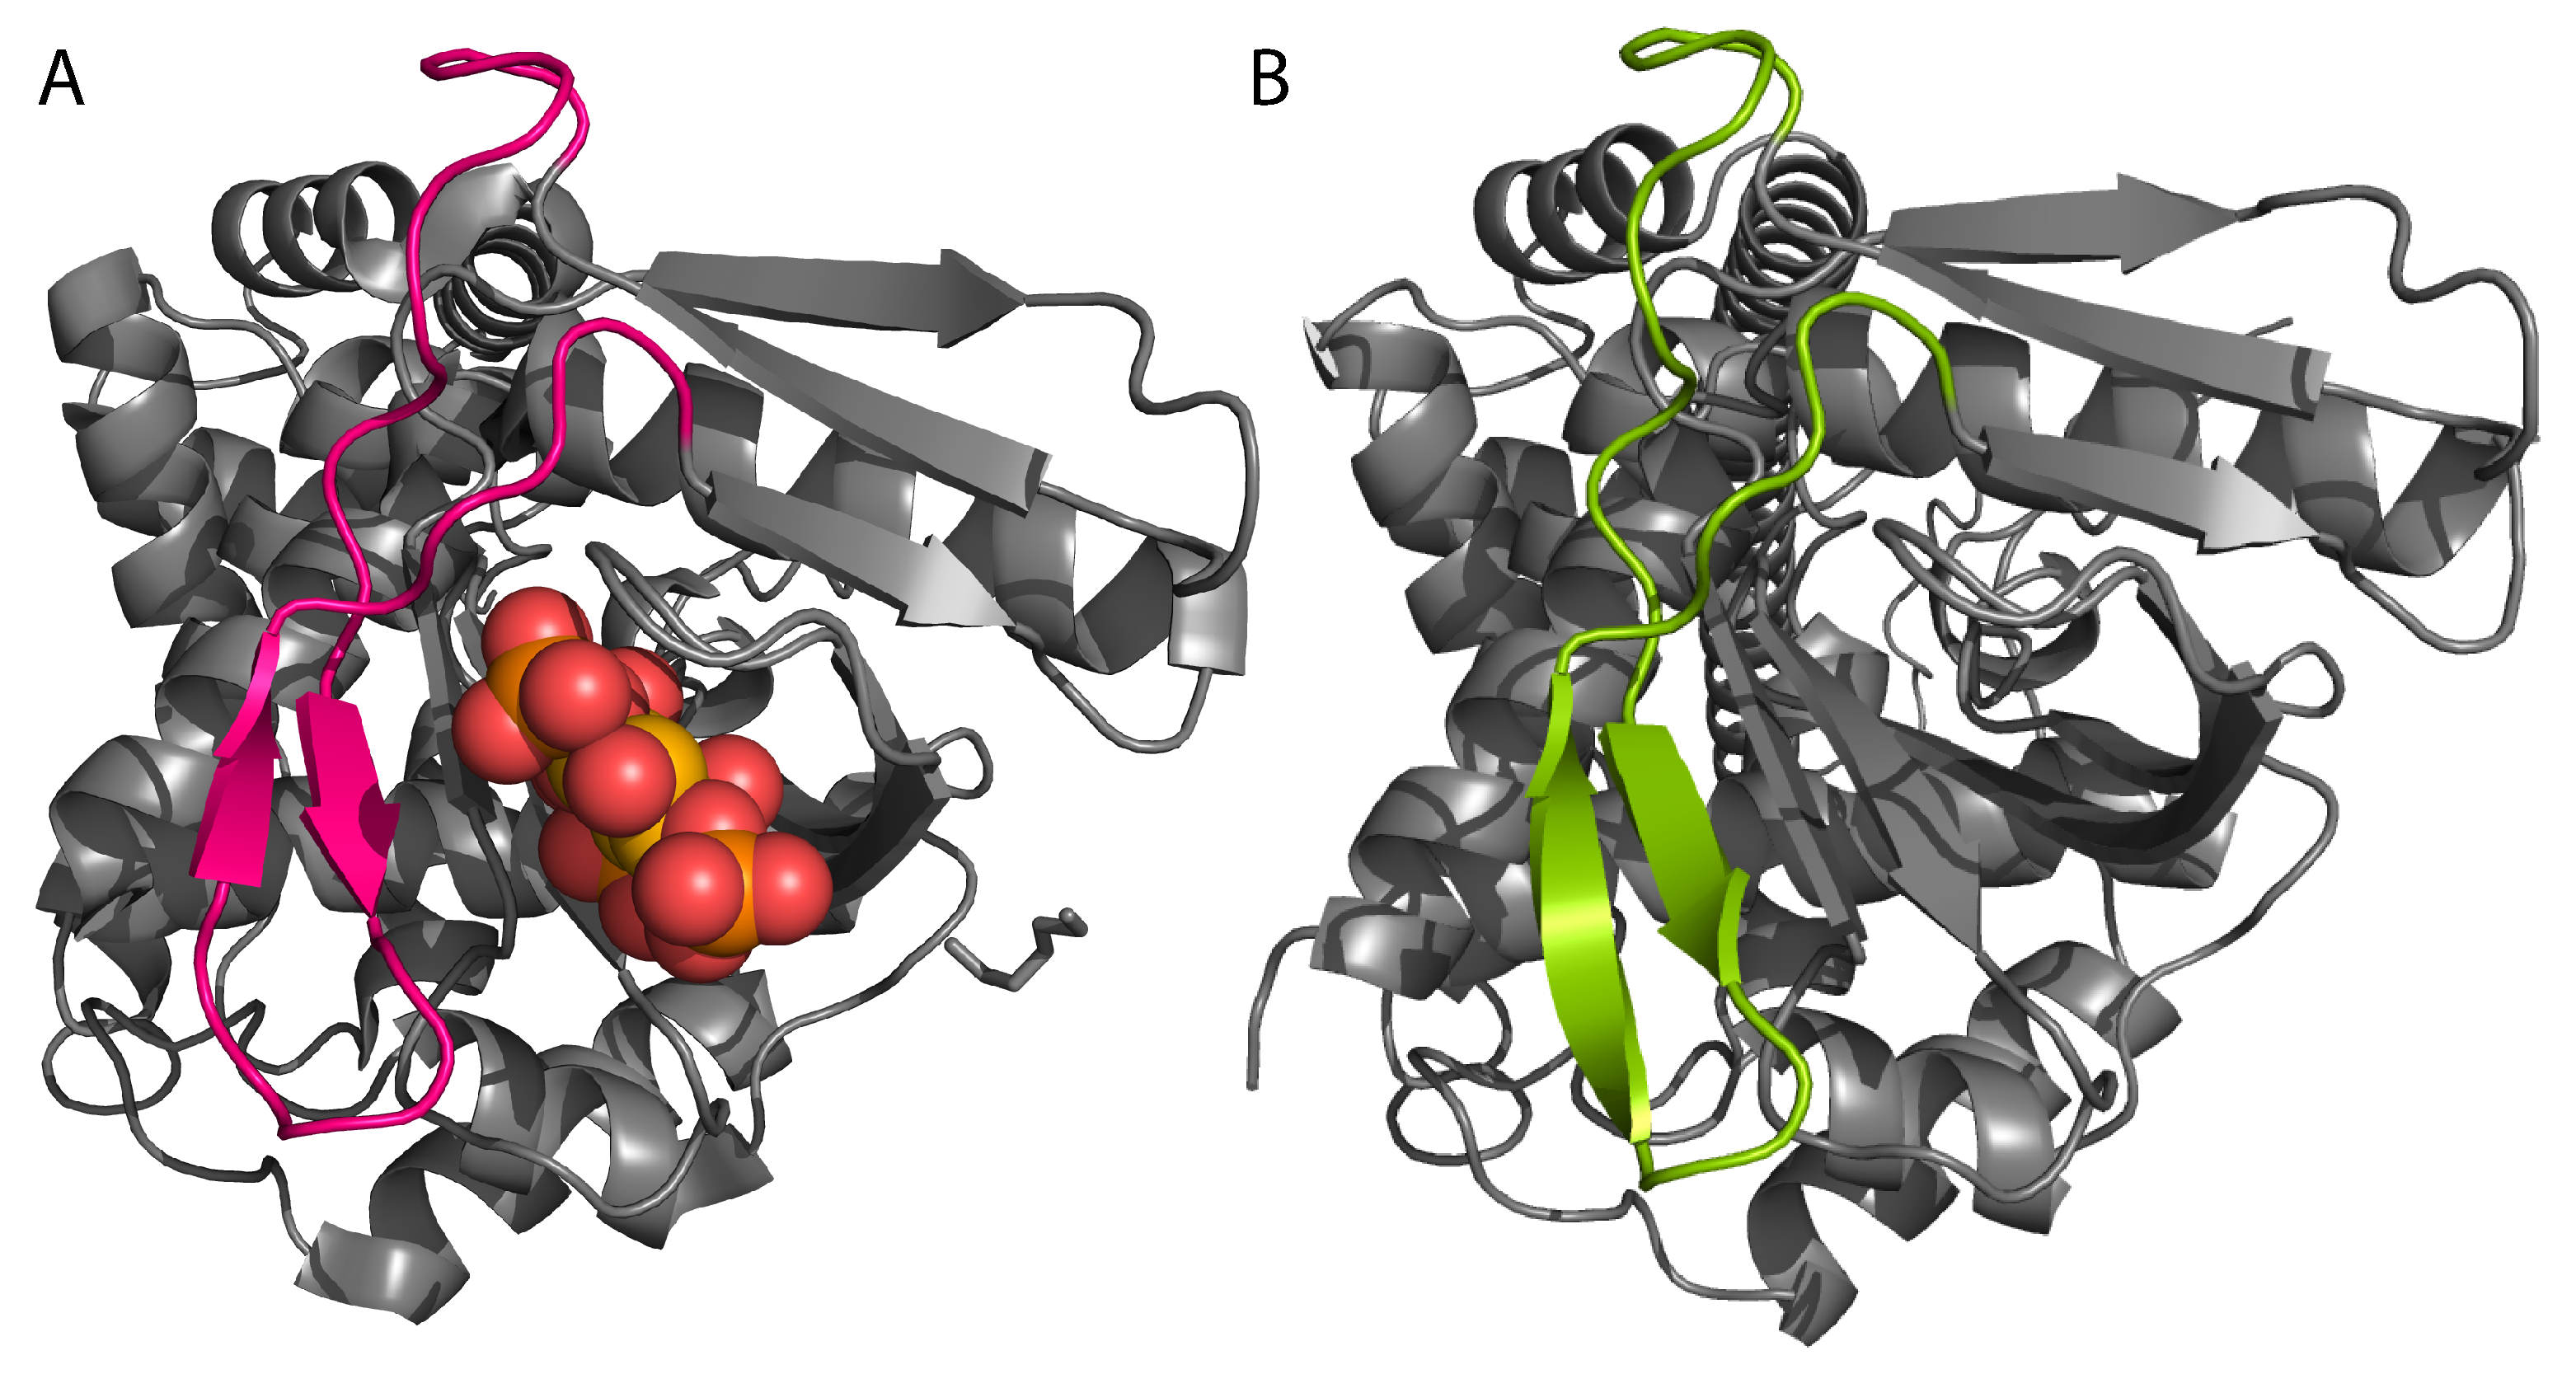
\includegraphics[width=1\linewidth]{figures/af3_pocket.pdf}
    \caption{\textbf{Mouse Cytohesin 3 binding pocket in experimental structure and AlphaFold3.} A) Experimental structure (PDB id: 2R0D \cite{dinitto_structural_2007}) with Ins(1,3,4,5)P\textsubscript{4} bound. Highlighted is the loop which features a long continuous segment of high pLDDT with ShiftCrypt values which show disorder. B) AlphaFold3 predicted structure. Highlighted is the same region as in A). The space occupied by Ins(1,3,4,5)P\textsubscript{4} in A) is present, in the absence of the ligand, in B).}
    \label{fig:discussion:af3_pocket}
\end{figure}


\subsection{pLDDT Does Not Accurately Reflect Gradations in Protein Dynamics}

We thereby find that pLDDT has a binary relationship with $S^{2}$ and $S^{2}_{\text{RCI}}$, where clearly rigid and clearly dynamic residues usually have high and low pLDDT values, respectively. Considering the largest dataset, with values for $S^{2}_{\text{RCI}}$, the overall correlation of pLDDT with $S^{2}_{\text{RCI}}$ is weak, especially when data is considered in strata (\tableref{table:pearson_metrics}). The stronger correlation for the full data spectrum than for strata indicates that pLDDT can better describe the extremes of protein \gls{dynamics}, but fails to describe fine gradations in \gls{dynamics}. Such results are coherent with the relation of pLDDT with predicted $S^{2}_{\text{RCI}}$, described in Chapter \ref{chapter:ambiguous} \cite{roca-martinez_challenges_2022}, where two high-density regions could be identified for predicted backbone \gls{dynamics} (\figref{fig:chapter5:fig5}). Constava's conformational state variability also shows similar trends, with only high pLDDT residues featuring low conformational state variability, but both mid and low pLDDT featuring predominantly high variability and low correlation along the whole range of values (\figref{fig:plddt_vs_conf_state_undivided}). This indicates a sharp change in behaviour from different pLDDT regions, rather than a gradation describing protein dynamic behaviour.

\subsection{Amino Acids with Multiple Conformations Tend to Feature Lower pLDDT}

In addition to pLDDT's relation to Constava's conformational state variability, we also observed that residues with the same secondary structure assignment across the entirety of the an NMR ensemble tend to have higher pLDDT values (Supplementary Fig. 5.10 A, D, G \& J). 
% (\suppfigref{fig:unique_and_or_cons} A, D, G \& J). 
Interestingly, this is also true for Coil and Turn, which are inherently unstructured, indicating that Coil and Turn residues that do not experience diversity in secondary structures are predicted more confidently by AlphaFold2 than those which do. Additionally, for every secondary structure type, those residues for which their predicted AlphaFold2 secondary structure matches the consensus secondary structure of the NMR ensemble also features higher pLDDT distributions than when these assignments mismatch (Supplementary Fig. 5.9 A, D \& G). 
% (\suppfigref{fig:af2_nmr_fold_missmatch} A, D \& G). 

Moreover, the match between AlphaFold2 and consensus NMR assignments results, for $\alpha$-Helix and $\beta$-Sheet, in higher pLDDT assignments than those with unique NMR assignments and mismatched AlphaFold2 assignments. The opposite is true for Coil and Turn residues, where a unique NMR assignment was more important than a matching AlphaFold2 assignment to obtain higher pLDDT distributions (Supplementary Fig. 5.11 A, D, G \& J).
% (\suppfigref{fig:unique_and_or_cons_match_af2} A, D, G \& J).
This is probably explained by the rigidisation of defined secondary structures into more stable forms under cryogenic conditions (\figref{fig:discussion:surrhelix_vs_xray}). AlphaFold replicates these rigid conformations and results in the assignment of the consensus NMR secondary structures, as it is the favourable one in cryogenic conditions. Overall, AlphaFold2 clearly shows a tendency for assigning higher pLDDT values to residues with unique secondary structure assignments across all structures in NMR structural ensembles.

Additionally, we have applied the Constava method to conformations generated with AlphaFlow \cite{jing_alphafold_2024}, a method that employs elements from AlphaFold's models to generate structural ensembles. Constava can be employed to compare structural ensembles and their conformational state propensities and variabilities, in this case between MD- and AlpaFlow-derived ensembles. From our limited testing, the ensembles generated with AlphaFlow seemed to overestimate protein conformational diversity compared to those obtained from MD simulations. This is reflected in more distributed conformational state propensities and therefore higher conformational state variability. Further, thorough testing is needed to assess more detailed differences between these ensembles and therefore the characteristics of AlphaFold-derived ensembles.


\section{Future Perspectives}

The work presented in this thesis opens the door to follow-up projects in several directions. The Constava software introduced new metrics to probabilistically describe protein conformation and its variability. This method is the product of several iterations, each with its own vision and strategies. During earlier stages, a branch of the project envisioned training a ML model to estimate Constava's metrics from amino acid sequence. Although these attempts were not immediately successful, they helped identify flaws in the definitions at each iteration. The final iteration of Constava focused on the description and thorough validation of the method, relegating the training of the estimator. While early attempts to create such an estimator have not yet achieved satisfactory performance, the project remains plausible. If these efforts succeed, we could see the expansion of bio2Byte Tools with a novel estimator of protein biophysics from amino acid sequences.

The expansion of bio2Byte Tools currently faces challenges arising from dependencies on crucial tools within the suite. These challenges have highlighted the necessity of generalising methods as much as possible and reducing external dependencies, particularly those lacking consistent updates to maintain compatibility with other contemporary software. A crucial and increasingly urgent task will be the re-implementation of multiple functions from obsolete dependencies into more generic code. Delaying this will likely result in the suite becoming another ``obsolete dependency'' itself. This is likely not a trivial process and will require the combined expertise of both technical and scientific staff.

Finally, the analysis of AlphaFold2's pLDDT leaves two immediate open paths for further research. First, a focused exploration of regions with conflicting NMR and AlphaFold \gls{dynamics} and conformations could provide deeper insights into the model's biases. We have shown general trends, supported by a key example illustrating the hypothetical effects of AlphaFold2's data processing pipeline, but further work could solidify and expand our interpretation. Secondly, some aspects of the study were limited by the daily job caps for generating AlphaFold3 predictions. It will be interesting to compare the current AlphaFold2 results with those of AlphaFold3 considering the recent publication of its code as open source \cite{callaway_ai_2024}. 
% when the method's code becomes public, the job cap is lifted, or a database with UniProt sequences is published, as was previously done for AlphaFold2.


\section{Closing Statement}

This thesis has introduced a new method to probabilistically describe protein conformation and its diversity, outlined a path for transforming outdated scientific tools into FAIR software, and explored the relationship between AlphaFold2 (and AlphaFold3, when possible) with protein \gls{dynamics} and conformation. The conclusions reached here open up new research avenues, some of which have been described above. These are aligned with the expertise and research lines of the bio2Byte group and will surely be further explored.



\begingroup
\small
\bibliographystyle{unsrt}
\bibliography{the_bibliography} 
\endgroup

% % % \chapter*{Supplementary information chapter \ref{chapter:constava}}
% \chapter*{Supplementary information chapter 3}
% \setcounter{chapter}{3}
% % \addcontentsline{toc}{chapter}{Supplementary information chapter \ref{chapter:constava}}
% \addcontentsline{toc}{chapter}{Supplementary information chapter 3}

% \markleft{S.I. Chapter 3}
% % \markboth{S.I. Chapter 3}

\chapter*{Supplementary information chapter 3}
\setcounter{chapter}{3}
% \addcontentsline{toc}{chapter}{Supplementary information chapter \ref{chapter:constava}}
\addcontentsline{toc}{chapter}{Supplementary information chapter 3}
\markright{SUPPLEMENTARY INFORMATION}

\begingroup
% Reset table and figure counters
\setcounter{table}{0}
\setcounter{figure}{0}

% Redefine table and figure captions
\captionsetup[table]{name=Supplementary Table}
\captionsetup[figure]{name=Supplementary Fig.}

\begin{figure}[H]
    \centering
    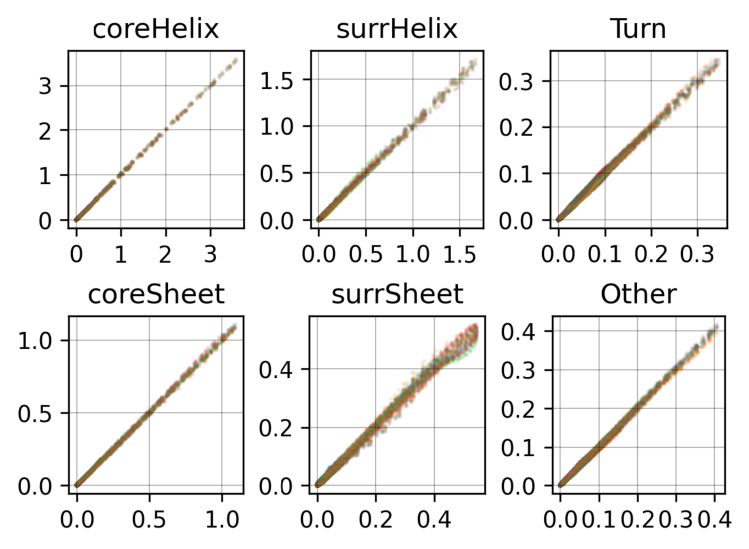
\includegraphics[width=\linewidth]{constava/sup_figs/supfig1.pdf}
    \caption{\textbf{Cross-validation of probability density kernels of conformational states.} The kernels were fitted five times, leaving out 20\% of the ensembles each time. The plots show the correlation between probability densities sampled from the five different kernels.}
    \label{fig:sup_fig_constava:cross_validation}
\end{figure}

\begin{figure}[H]
    \centering
    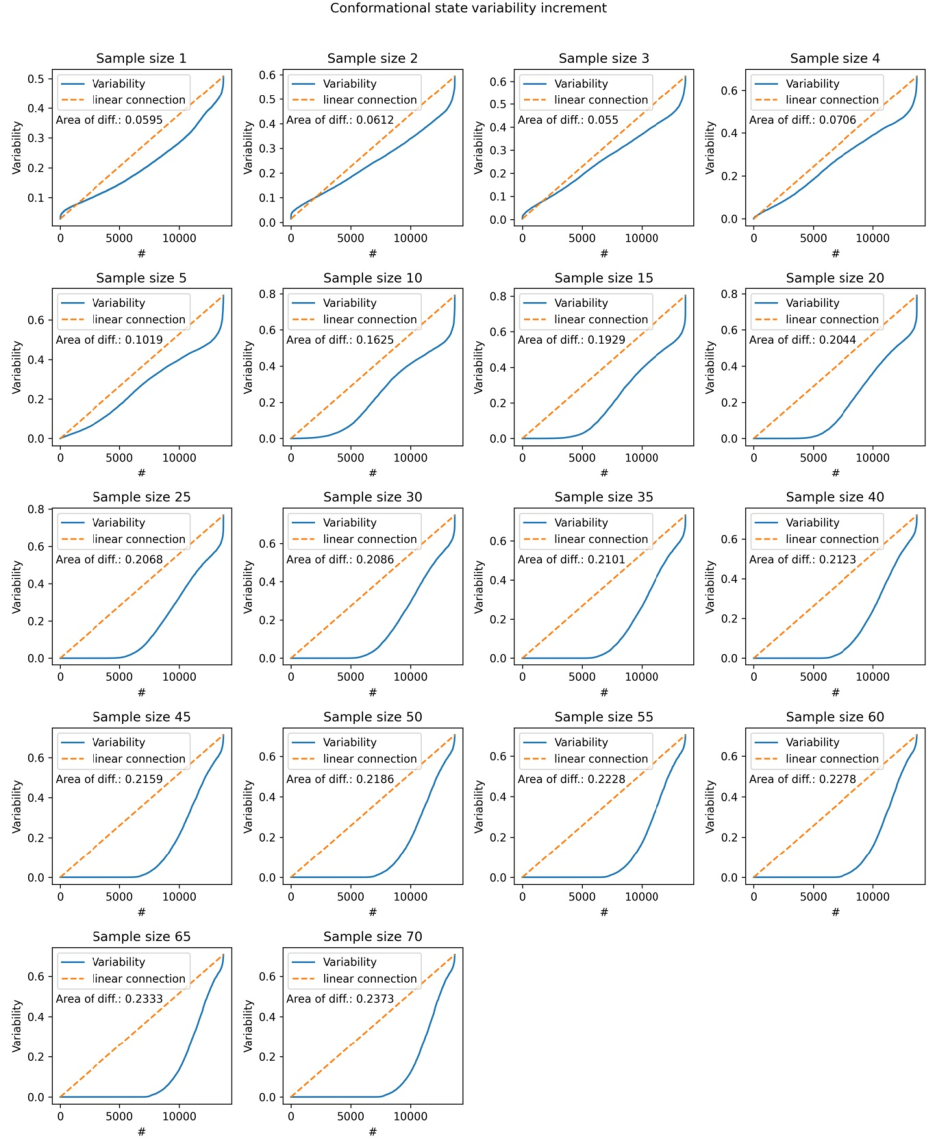
\includegraphics[width=0.9\linewidth]{constava//sup_figs/supfig2.pdf}
    \caption{\textbf{Influence of the sample size on the conformational state variability.} Conformational state variabilities were calculated for all residues in the MD ensembles employing bootstrapping with different sample sizes (10,000 samples). The resulting values were plotted in ascending order (blue), while the dashed line (orange) represents an ideal line between the minimum and maximum values. Thus, the area between the two lines is a measure of the linearity of the conformational state variability in the dataset. As the sample size increases, less samples fall in the linear section of the conformational state variability metric. A sample size of 3 was chosen to obtain informative conformational state variabilities from ensembles for presenting the highest linearity in the metric while also spanning over a decent value range (min-max, see \suppfigref{fig:sup_fig_constava:range}).}
    \label{fig:sup_fig_constava:sample_size}
\end{figure}

\begin{figure}[H]
    \centering
    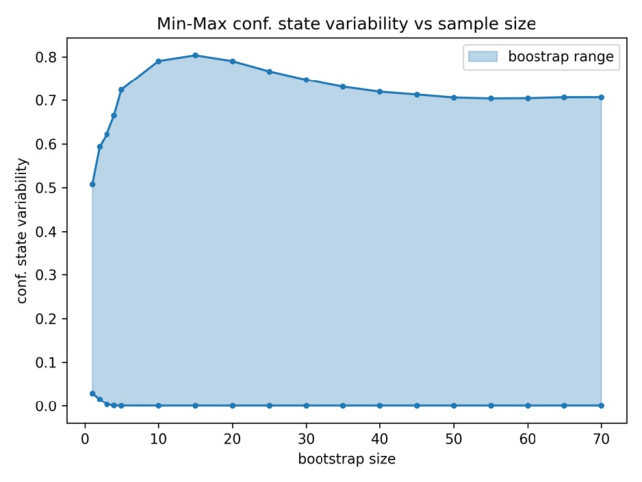
\includegraphics[width=0.9\linewidth]{constava//sup_figs/supfig3.pdf}
    \caption{\textbf{Range of conformational state variability values as a function of the sample size.} Conformational state variabilities were calculated for all residues in the MD ensembles employing bootstrapping with different sample sizes (10,000 samples). The minimum and maximum values are shown here. Initially, as the sample size increases, the range between minimum and maximum values increases as well, reaching a maximum at a sample size of 15. For low sample sizes, conformational state variabilities of 0 are practically not observed. This indicates that even smallest fluctuations of the backbone dihedrals lead to an increase in conformational state variability. As the sample size increase, those small fluctuations become less important, allowing for conformational state variabilities that are practically 0.}
    \label{fig:sup_fig_constava:range}
\end{figure}

\begin{figure}[H]
    \centering
    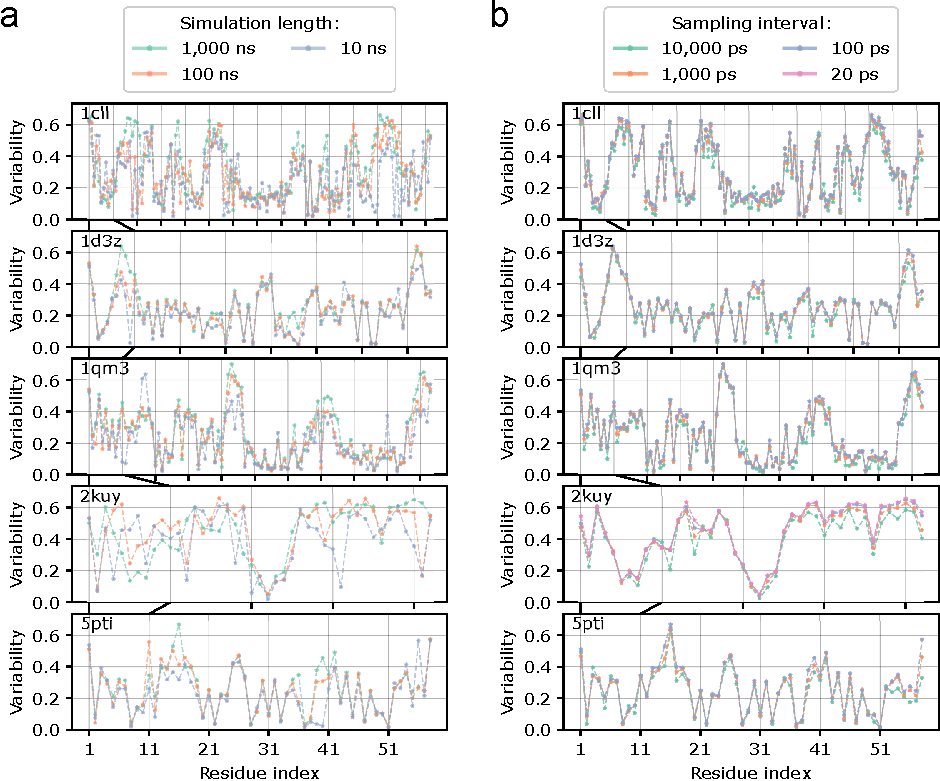
\includegraphics[width=1\linewidth]{constava//sup_figs/supfig4.pdf}
    \caption{\textbf{Analysis of sampling parameters for molecular dynamics simulations.} Five proteins were simulated to assess the impact of different sampling parameters on the results. From all simulations the conformational state variabilities were calculated using the sliding window-approach with a window size of 3. Results are shown as the conformational state variability along the sequence for different sampling parameters. a) Analysis of the of the impact of simulation time. Results after 100 ns did not differ much from longer simulations. b) Analysis of the impact of sampling intervals. Only minor changes were observed. Sampling in intervals of 1,000 ps was chosen for the final simulations in this work, to minimize the autocorrelation between subsequent sampling time points.}
    \label{fig:sup_fig_constava:MD_parameters}
\end{figure}

\begin{figure}[H]
    \centering
    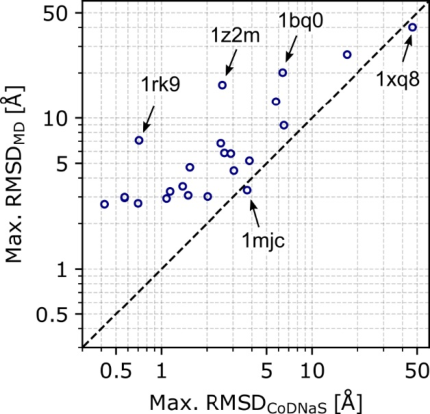
\includegraphics[width=0.7\linewidth]{constava//sup_figs/supfig5.pdf}
    \caption{\textbf{Comparison of conformational diversity between MD ensembles and CoDNaS.} For a given protein the maximum RMSD values between any structures in CoDNaS (x-axis) and the MD ensemble (y-axis) are depicted. With two exceptions (1mjc and 1xq8) the MD simulations produced more diverse ensembles than the structures in CoDNaS. For some structures (e.g., 1z2m and 1bq0) the conformational variability in the simulation strongly exceeded that in CoDNaS. This is mostly due to flexible termini, which MD simulations sample freely. A notable exception is 1rk9, which remains fully folded throughout the simulation but undergoes a conformational change which results in a higher RMSD than observed in CoDNaS. Out of the 113 simulated proteins, only 22 are annotated in CoDNaS.}
    \label{fig:sup_fig_constava:codnas}
\end{figure}

\begin{figure}[H]
    \centering
    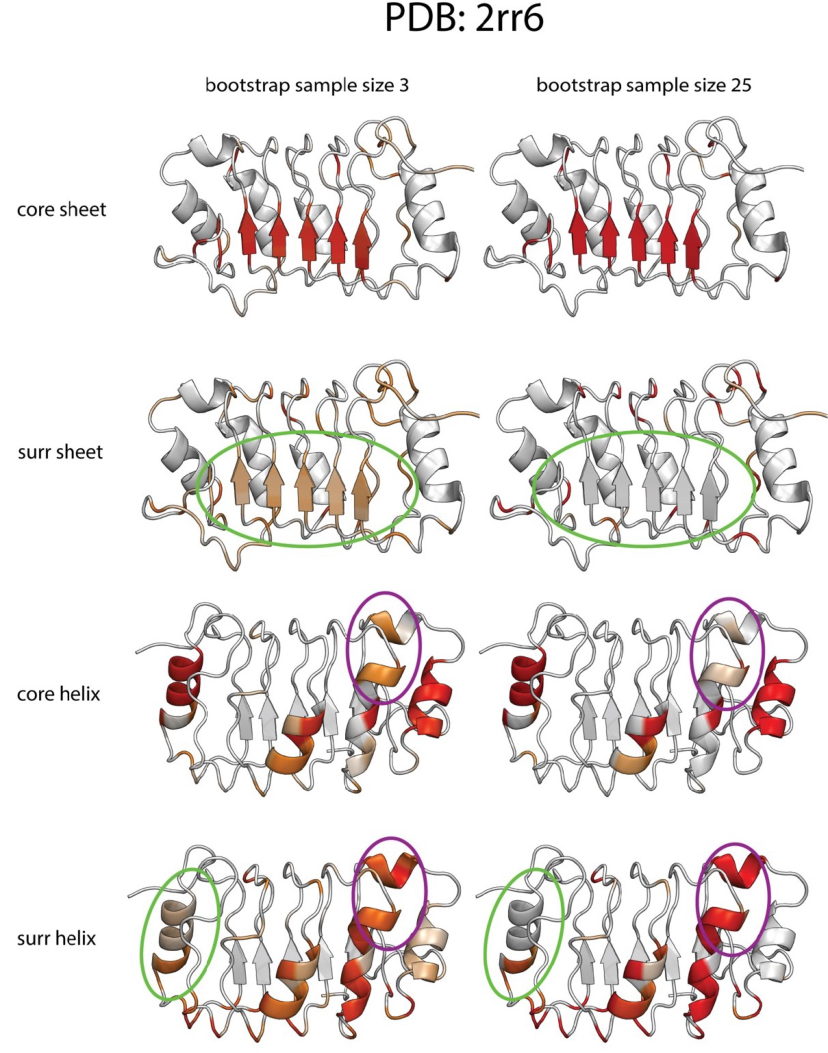
\includegraphics[width=0.8\linewidth]{constava//sup_figs/supfig6.pdf}
    \caption{\textbf{Impact of the sample size on conformational states probabilities in human acidic leucine-rich nuclear phosphoprotein 32 family member B (PDB ID: 2rr6).} Conformational state propensities were inferred from the MD ensembles employing bootstrapping with sample sizes 3 and 25 (10,000 samples). As the sample size increases, ambiguous assignments (shades of orange) become less apparent, rather a preferred conformational state is assigned with high propensity (shades of red). On the first two rows, the low probability for Surrounding sheet in the circled area disappears in favour of higher probabilities towards Core sheet. Similarly, in the last two rows the green circled region experiences an increase in Core helix probability. Contrarily, the purple circled region experiences an increase Surrounding helix probability in detriment of Core helix probability.}
    \label{fig:sup_fig_constava:bootstrap_size}
\end{figure}

\begin{figure}[H]
    \centering
    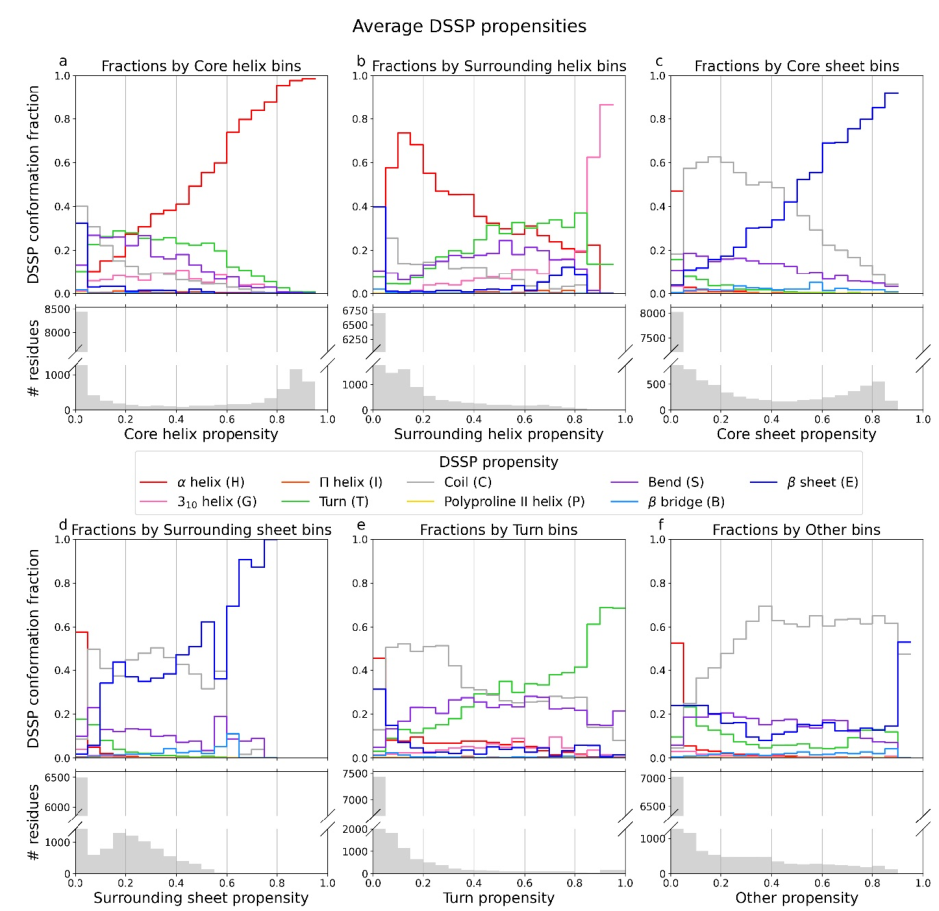
\includegraphics[width=0.9\linewidth]{constava//sup_figs/supfig7.pdf}
    \caption{\textbf{Relation between Constava conformational states and DSSP secondary structure assignments.} Constava conformational state propensities were correlated with DSSP propensities (average fraction of frames assigned to a given secondary structure by DSSP). The two classification schemes were compared in bins. The bar plot below the correlation plots shows the number of samples (residues) in each bin. a) For Core helix propensities there is a correlation to H ($\alpha$-helix). b) For Surrounding helix propensities no clear correlations to any DSSP category can be observed. The values for bins with propensities > 0.8 cannot be properly interpreted due to the low number of samples. c) For Core sheet there is a correlation with E ($\beta$-sheet). d) For Surrounding sheet no clear correlations are apparent. There is some correlation with E, but the relationship is non-linear and the low number of samples for propensities > 0.6 makes the interpretation difficult. e) For Turn a correlation with T (hydrogen bonded turns) emerges but other DSSP categories are observed for all levels of Turn propensity. f) Finally, the Other propensity mostly associates to C (coil), but also other DSSP categories are observed for all levels of Other propensity. Since Turn and Other indicate highly dynamic residues, it makes sense, that these residues form other secondary structure elements transiently.}
    \label{fig:sup_fig_constava:dssp_assignments}
\end{figure}

\begin{figure}[H]
    \centering
    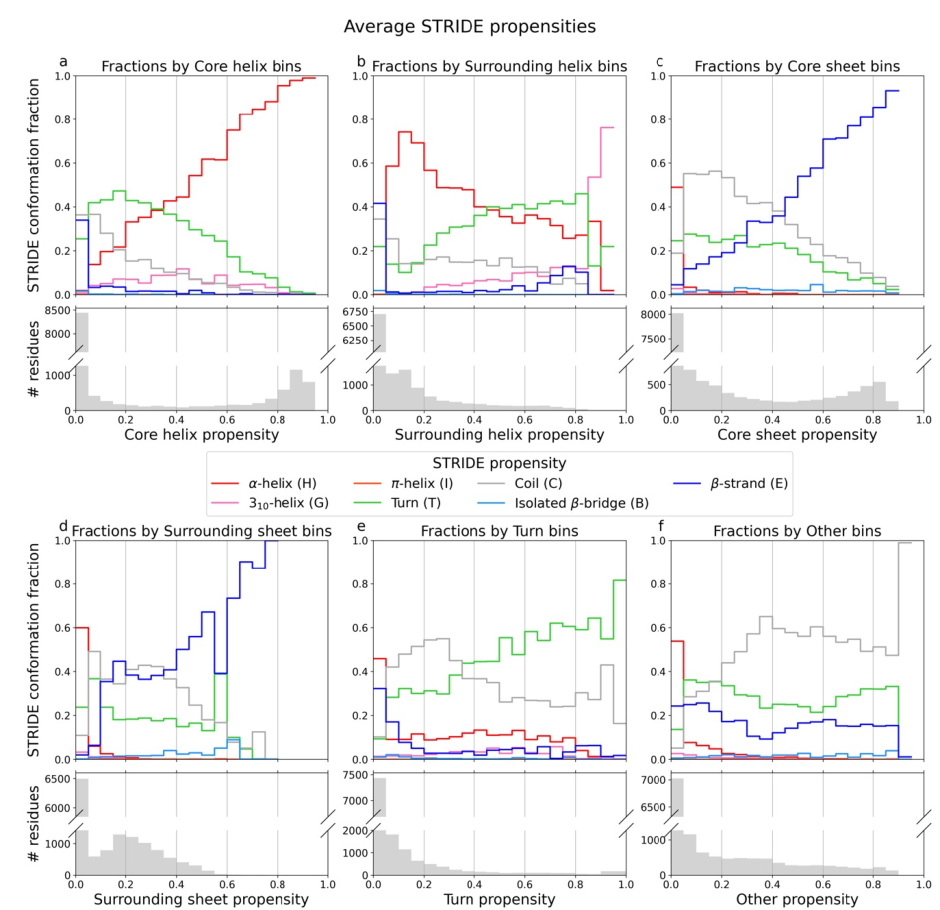
\includegraphics[width=0.9\linewidth]{constava//sup_figs/supfig8.pdf}
    \caption{\textbf{Relation between Constava conformational states and STRIDE secondary structure assignments.} Constava conformational state propensities were correlated with STRIDE propensities (average fraction of frames assigned to a given secondary structure by STRIDE). The two classification schemes were compared in bins. The bar plot below the correlation plots shows the number of samples (residues) in each bin. a) For Core helix propensities there is a correlation to H ($\alpha$-helix). b) For Surrounding helix propensities no clear correlations to any STRIDE category can be observed. The values for bins with propensities > 0.8 cannot be properly interpreted due to the low number of samples. c) For Core sheet there is a correlation with E ($\beta$-sheet). d) For Surrounding sheet no clear correlations are apparent. There is some correlation with E, but the relationship is non-linear and the low number of samples for propensities > 0.6 makes the interpretation difficult. e) For Turn a correlation with T (hydrogen bonded turns) emerges but other STRIDE categories are observed for all levels of Turn propensity. f) Finally, the Other propensity mostly associates to C (coil), but also other STRIDE categories are observed for all levels of Other propensity. Since Turn and Other indicate highly dynamic residues, it makes sense, that these residues form other secondary structure elements transiently.}
    \label{fig:sup_fig_constava:stride_assignments}
\end{figure}

\begin{figure}[H]
    \centering
    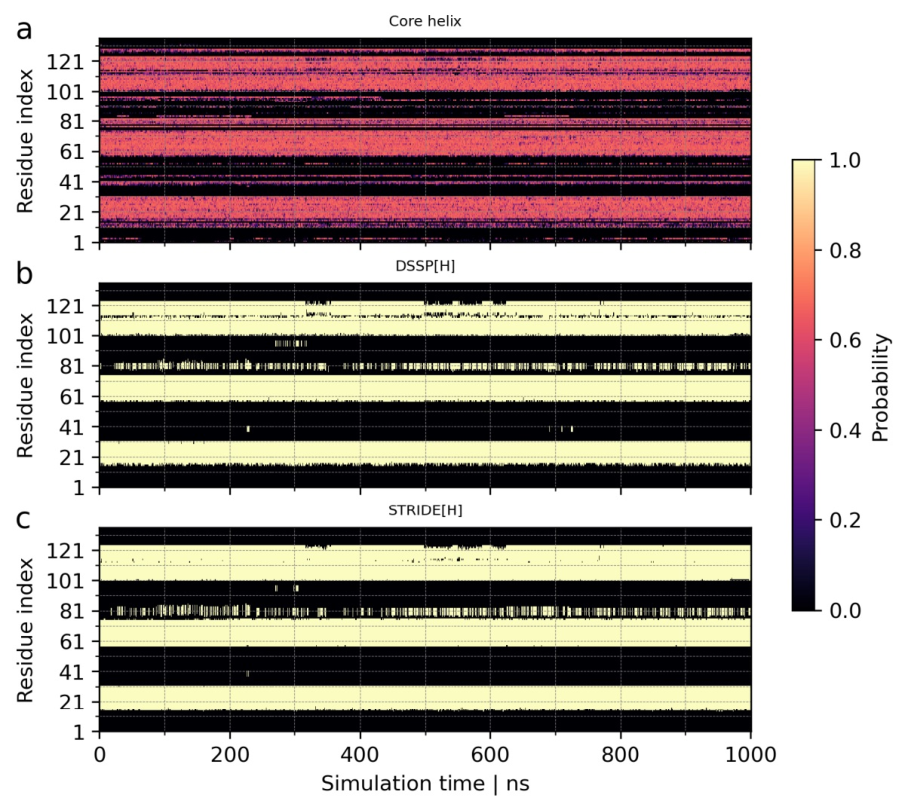
\includegraphics[width=\linewidth]{constava//sup_figs/supfig9.pdf}
    \caption{\textbf{Comparison of Constava and traditional secondary structure assignments with respect to their ability to detect transiently forming secondary structure elements. }
    % Constava, DSSP, and STRIDE were applied to all conformations in the MD trajectories. Shown are: a) Core helix propensities, b) DSSP H ($\alpha$-helix) assignments, and c) STRIDE H ($\alpha$-helix) assignments along the MD trajectory of Endonuclease V (PDB ID: 2end). Beyond the relation between propensities and fractions in Supplementary Fig. 7 and Supplementary Fig. 8, Constava shows the capability to detect conformational states before the criteria for the other methods are met. In addition to returning high Core helix probability to the stable helix regions that DSSP and STRIDE assign, some regions with more dynamic behaviour interestingly show detection of helix propensity. The region between amino acids 95-101 is detected to have notable Core helix propensity (a) by Constava throughout the totality of the simulation, even though it is rarely assigned by DSSP (b) and STRIDE (c) in the MD time steps. Additionally, the region between amino acids 39-45 shows a similar tendency, with a longer amino acid range of high Core helix propensities near in the 300 ns time step, where DSSP and STRIDE detect $\alpha$-helix. This longer stretch indicates that enough amino acids to form the necessary hydrogen bonds for DSSP and STRIDE assignment have adopted Core helix conformation. Finally, the region between amino acids 55-60 is also detected along the whole simulation, while DSSP and STRIDE intermittently assigns $\alpha$-helix.
    }
    \label{fig:sup_fig_constava:detect_trasient}
\end{figure}

\begin{figure}[H]
  \ContinuedFloat
  \caption[]{(Continuation) Constava, DSSP, and STRIDE were applied to all conformations in the MD trajectories. Shown are: a) Core helix propensities, b) DSSP H ($\alpha$-helix) assignments, and c) STRIDE H ($\alpha$-helix) assignments along the MD trajectory of Endonuclease V (PDB ID: 2end). Beyond the relation between propensities and fractions in Supplementary Fig. 7 and Supplementary Fig. 8, Constava shows the capability to detect conformational states before the criteria for the other methods are met. In addition to returning high Core helix probability to the stable helix regions that DSSP and STRIDE assign, some regions with more dynamic behaviour interestingly show detection of helix propensity. The region between amino acids 95-101 is detected to have notable Core helix propensity (a) by Constava throughout the totality of the simulation, even though it is rarely assigned by DSSP (b) and STRIDE (c) in the MD time steps. Additionally, the region between amino acids 39-45 shows a similar tendency, with a longer amino acid range of high Core helix propensities near in the 300 ns time step, where DSSP and STRIDE detect $\alpha$-helix. This longer stretch indicates that enough amino acids to form the necessary hydrogen bonds for DSSP and STRIDE assignment have adopted Core helix conformation. Finally, the region between amino acids 55-60 is also detected along the whole simulation, while DSSP and STRIDE intermittently assigns $\alpha$-helix.}
\end{figure}

\begin{figure}[H]
    \centering
    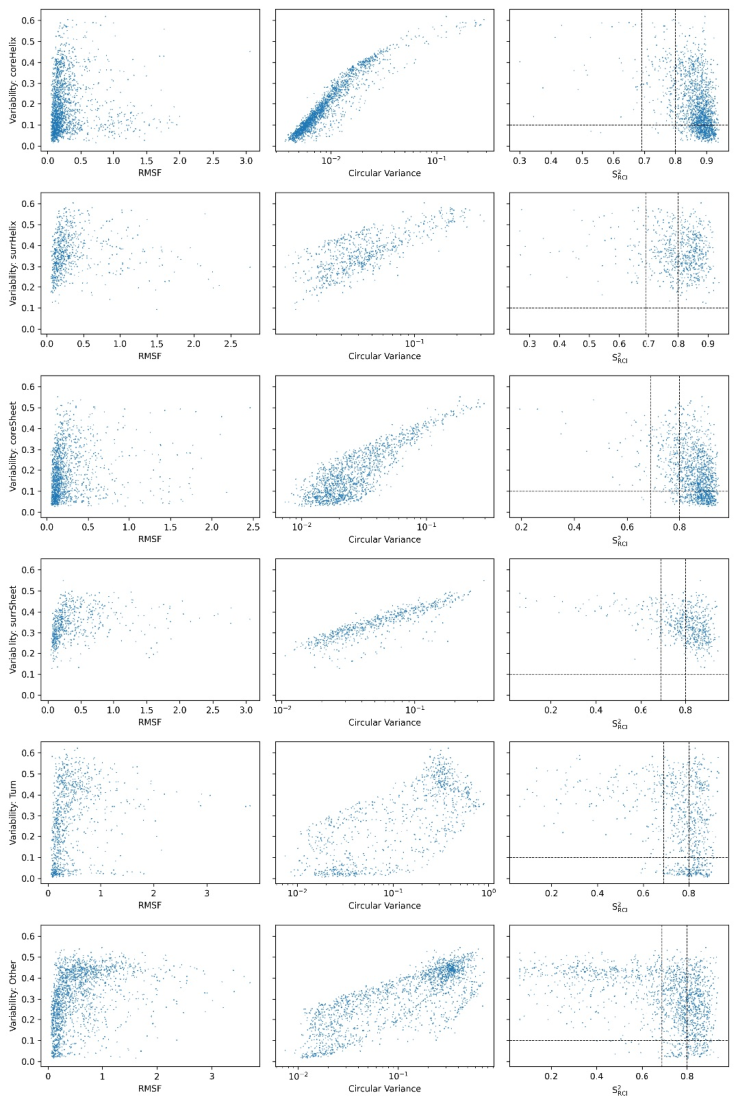
\includegraphics[width=0.85\linewidth]{constava//sup_figs/supfig10.pdf}
    \caption{\textbf{Comparison of conformational state variability with traditional dynamics metrics per prevalent conformational state.} 
    % Conformational state propensities were inferred from the MD ensembles employing bootstrapping with sample sizes 3 (10,000 samples). The results were subdivided by their prevalent conformational state. From top to bottom these are: Core helix, Surrounding helix, Core sheet, Surrounding sheet, Turn and Other. In the left column, the conformational state variability is potted against the root mean square fluctuations (RMSF). In the central column, the conformational state variability is plotted against the circular variance. On the right, the conformational state variability is plotted against the $\text{S}^{2}_{RCI}$. The vertical dotted lines indicate the border between likely disordered, context-dependent and ordered residues (left to right) as defined in previous work [1]. The horizontal dotted line is a visual guide to distinguish between residues with very low and higher conformational state variability.
    }
    \label{fig:sup_fig_constava:metrics}
\end{figure}

\begin{figure}[H]
  \ContinuedFloat
  \caption[]{(Continuation) Conformational state propensities were inferred from the MD ensembles employing bootstrapping with sample sizes 3 (10,000 samples). The results were subdivided by their prevalent conformational state. From top to bottom these are: Core helix, Surrounding helix, Core sheet, Surrounding sheet, Turn and Other. In the left column, the conformational state variability is potted against the root mean square fluctuations (RMSF). In the central column, the conformational state variability is plotted against the circular variance. On the right, the conformational state variability is plotted against the $\text{S}^{2}_{RCI}$. The vertical dotted lines indicate the border between likely disordered, context-dependent and ordered residues (left to right) as defined in previous work [1]. The horizontal dotted line is a visual guide to distinguish between residues with very low and higher conformational state variability.}
\end{figure}

\begin{figure}[H]
    \centering
    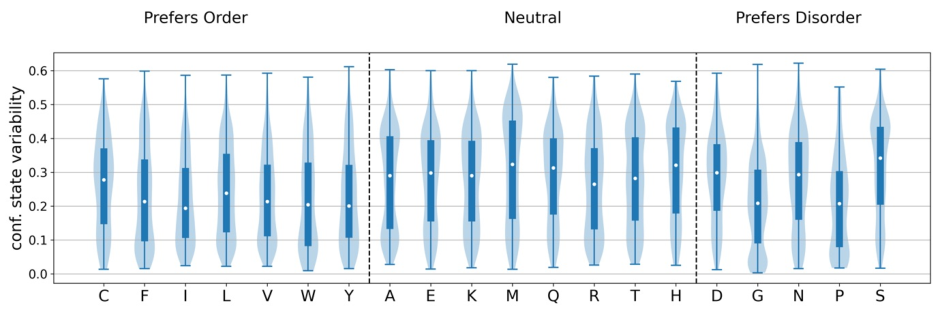
\includegraphics[width=1\linewidth]{constava//sup_figs/supfig11.pdf}
    \caption{\textbf{Conformational state variability values per amino acid type according to their order preference, terminal regions included.} Conformational state variabilities were calculated for all residues in the MD ensembles employing bootstrapping with sample size 3 (10,000 samples). Amino acids were classified depending on their intrinsic order preference according to the classification on previous work1 as preferentially ordered (cysteine, phenylalanine, isoleucine, leucine, valine, tryptophan \& tyrosine), neutral (alanine, glutamic acid, lysine, methionine, glutamine, arginine, threonine \& histidine) and preferentially disordered (aspartic acid, glycine, asparagine, proline \& serine). Amino acids which prefer order generally featured lower conformational state variability values than the remaining. The homologous figure with terminal residues removed can be found in the main text, Figure 5. This figure mainly differs in the variability values distribution for methionine, which features higher values in this figure than in Figure 6. This is due to the preferential location of Methionine at the N-terminal region of the protein, which is less bound to inter-residue interactions and allows for easier conformational state changes and therefore variability.}
    \label{fig:sup_fig_constava:aa_order}
\end{figure}

\begin{figure}[H]
    \centering
    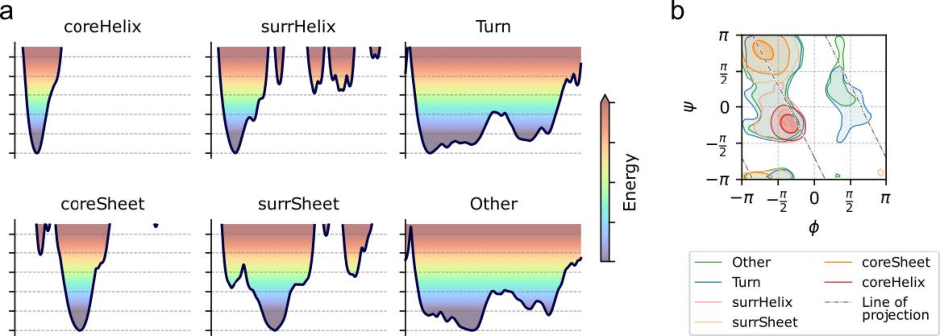
\includegraphics[width=1\linewidth]{constava//sup_figs/supfig12.pdf}
    \caption{\textbf{Schematic representation of the conformational states as energy landscapes.} a) Cross section through the energy landscapes along the line of projection (shown in panel b). coreHelix and coreSheet conformational states are defined by a single deep energy well, vastly restricting backbone mobility. The states surrHelix and surrSheet show lowered energy barriers, allowing for more backbone mobility. Finally, in the Other and Turn conformational states, most of the dihedral space is accessible with only minor energy barriers in between. b) Schematic overview of the definition of the conformational states, as well as the line of projection used in panel a.}
    \label{fig:sup_fig_constava:2d_landscape}
\end{figure}

\begin{figure}[H]
    \centering
    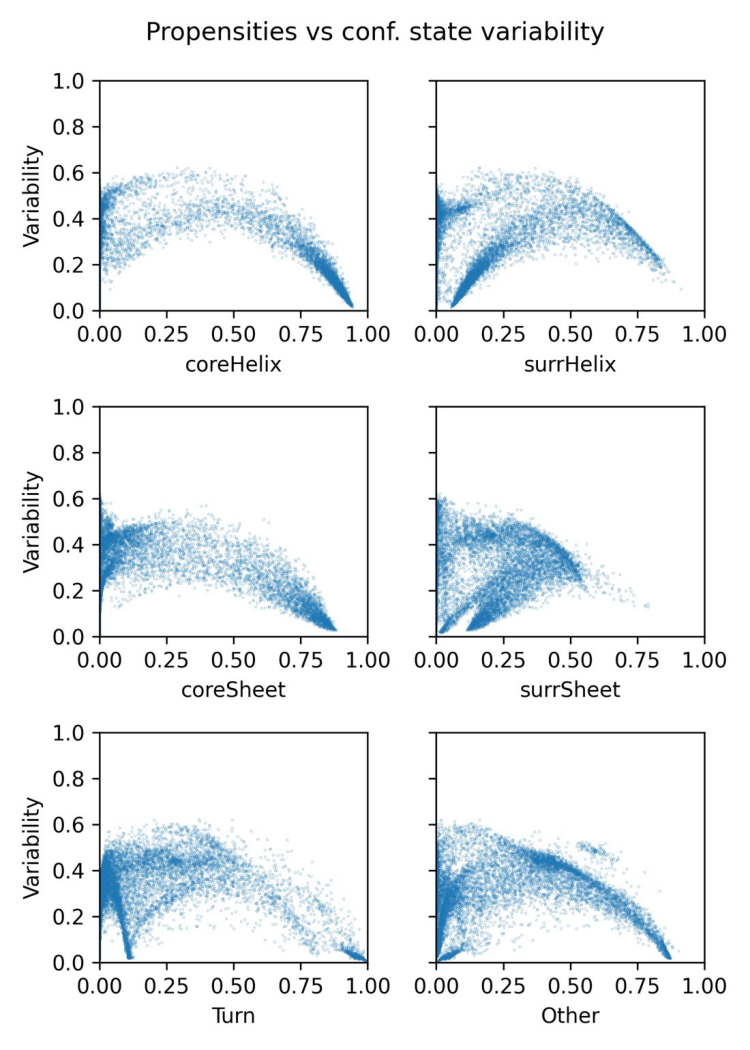
\includegraphics[width=0.8\linewidth]{constava//sup_figs/supfig13.pdf}
    \caption{\textbf{Conformational states propensities vs conformational state variability.} The metrics were calculated using bootstrapping with a sample size of 3 (10,000 samples). Conformational state propensities for each conformational state are plotted on the x axes, while the y axes show the conformational state variability. As the conformational state propensity for a single conformational state approaches 1, the conformational state variability drops to 0. In contrast, no such correlation can be observed in the left half of the plots. As the probability for a given conformational state approaches 0, the residue may still assume any of the remaining five states, and transition between them, thus, allowing for no conclusions on the conformational state variability.}
    \label{fig:sup_fig_constava:var_vs_propensity}
\end{figure}

\begin{figure}[H]
    \centering
    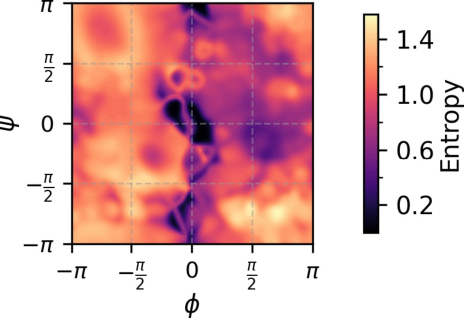
\includegraphics[width=0.8\linewidth]{constava//sup_figs/supfig14.pdf}
    \caption{\textbf{Entropy of the conformational states in the ($\phi$, $\psi$)-space.} The entropy is a measure of how sensitive the conformational states are to minor changes in the backbone dihedrals in the corresponding areas. The area around (0, 0) is not populated in any of the conformational state models. Thus, the entropy in this region approaches 0.}
    \label{fig:sup_fig_constava:entropy}
\end{figure}

\begin{figure}[H]
    \centering
    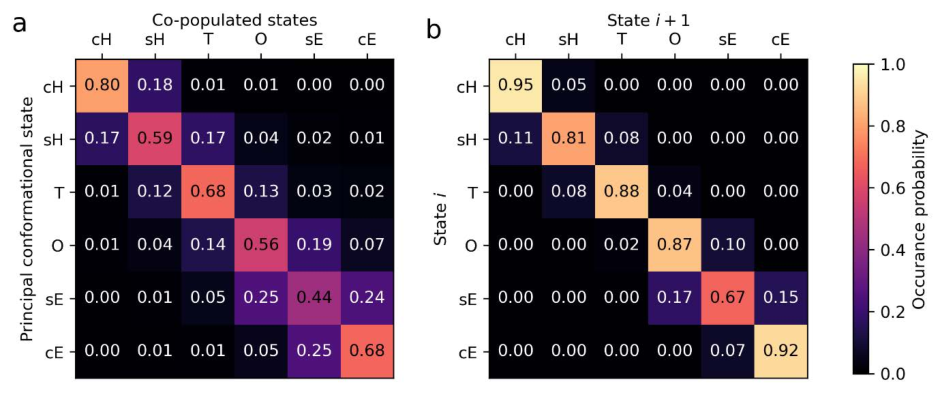
\includegraphics[width=1\linewidth]{constava//sup_figs/supfig15.pdf}
    \caption{\textbf{Co-occurrence of conformational states.} a) This plot shows the overall co-occurrence of conformational states in individual residues. For every residue with a given most likely conformational state (vertical axis), the average remaining propensities for all other states are shown (horizontal axis). b) This plot shows the probabilities of residues transitioning between conformational states between two subsequent time points. Both plots were obtained with window size 3. The labels correspond to the conformational states as follows: cH (Core helix), sH (Surrounding helix), T (Turn), O (Other), sE (Surrounding sheet), cE (Core sheet).}
    \label{fig:sup_fig_constava:co-occurrence}
\end{figure}

\newpage

\begin{suppdata} \label{data:sup_data_constava:order_class_proteins}
\textbf{List of proteins according to order class.}\\

\noindent\textbf{Disordered:} 2aqc, 1xq8, 1mjc, 1u96, 1ss3, 2kbz, 2l95, 1nq4, 1vd0, 1y00, 1rk9, 2l50, 1yob, 1rqs, 1czh.\\
\textbf{Half-disordered:} 2jo6, 2rvh, 2khz, 1akp, 2m2u, 2ho9, 2m9v, 2joy, 2mlw, 2lnu, 1b75, 2ot2, 1c9h, 2l7w, 1r1t, 2l49, 2l9n, 2myi, 2ls7, 1o13, 2lvh, 2l6o, 5vo7, 2kly, 2l25, 1wm2, 2kpq, 2kg7, 1l7y, 2gqb, 1eni, 1z2m, 2den, 2jra, 2jyz, 2jz4, 2m0y, 2m2a, 2mc9, 2mhe, 2mvz, 2x8n, 4beh, 4eyv, 5jtk.\\
\textbf{Structured:} 2mkx, 1jqr, 2fm4, 1jw3, 2rr6, 1hg7, 1sp0, 2kva, 3hnx, 1tm9, 1om2, 2d49, 2hfi, 1ufn, 1qkh, 2fvt, 1rzs, 1x3a, 1ey1, 1wjt, 2hgk, 2k2t, 2jny, 2jso, 2rn4, 1bq0, 1g9l, 1imq, 1iyr, 1jh3, 1jw2, 1mp1, 1nnv, 1nzp, 1rq6, 1rrz, 1ryk, 1t0g, 1tl6, 1v66, 1v9v, 1xhs, 2ebm, 2end, 2gbs, 2hfq, 2jgx, 2jov, 2jrr, 2jv2, 2jzv, 2ken, 2lfj.
\end{suppdata}

\begin{suppdata} \label{data:sup_data_constava:prots_with_nmr_metrics}
\textbf{List of proteins mapped to NMR metrics.} Only the following subset of MD proteins had their corresponding Random Coil Index information available:\\

\noindent2m2a, 1jw2, 2ls7, 1t0g, 2jny, 1tm9, 1v66, 2gqb, 2ebm, 2kpq, 1ryk, 2gbs, 2fvt, 2ken, 1b75, 2l25, 2rr6, 1iyr, 2hfi, 2ho9, 1akp, 2fm4, 1xhs, 1l7y, 1ufn, 2mlw, 1ey1, 2kva, 2mvz, 2lnu, 2lfj, 1om2, 2jyz, 2mhe, 1v9v, 2l49, 1jqr, 1x3a, 1g9l, 2rvh, 5vo7, 1bq0, 2l6o, 1c9h, 2jov, 2ot2, 2joy, 2rn4, 2hgk, 1jh3, 2jz4, 5jtk, 1rzs, 2jso, 2kbz, 1rq6, 2jzv, 1wjt, 1jw3, 2jrr, 1hg7, 1imq.
\end{suppdata}
% % \chapter*{Supplementary information chapter \ref{chapter:b2btools_deployment}}
\chapter*{Supplementary information chapter 6}
\setcounter{chapter}{6}
% \addcontentsline{toc}{chapter}{Supplementary information chapter \ref{chapter:b2btools_deployment}}
\addcontentsline{toc}{chapter}{Supplementary information chapter 6}
\markright{SUPPLEMENTARY INFORMATION}

\begingroup
% Reset table and figure counters
\setcounter{table}{0}
\setcounter{figure}{0}

% Redefine table and figure captions
\captionsetup[table]{name=Supplementary Table}
\captionsetup[figure]{name=Supplementary Fig.}


\begin{table}[ht]
\centering
\small
% \captionsetup{justification=centering}
\caption{\textbf{Tools description.} Simple description of every tool contained in bio2Byte tools.}
\label{tab:tool_explanation}
% \begin{tabular}{c p{10cm}}
% \begin{tabular}{>{\raggedright}m{1.5cm} p{10cm}} % Use 'm' column type for vertical alignment control
\begin{tabular}{>{\raggedright\arraybackslash}p{1.5cm} >{\raggedright\arraybackslash}p{10cm}} % Ensuring top alignment
\toprule
\textbf{\color{black} Predictor} & \textbf{\color{black} Usage} \\ \midrule
\color{black} DynaMine & \color{black} Fast predictor of protein backbone dynamics using only sequence information as input. The current version also predicts side-chain dynamics and secondary structure predictors using the same principle. \\ %\hline
\color{black} DisoMine & \color{black} Predicts protein disorder with recurrent neural networks not directly from the amino acid sequence, but instead from more generic predictions of key biophysical properties, here protein dynamics, secondary structure and early folding. \\ %\hline
\color{black} EfoldMine & \color{black} Predicts from the primary amino acid sequence of a protein, which amino acids are likely involved in early folding events. \\ %\hline
\color{black} AgMata & \color{black} Single-sequence based predictor of protein regions that are likely to cause beta-aggregation. \\ %\hline
\color{black} PSPer & \color{black} PSP (Phase Separating Protein) predicts whether a protein is likely to phase-separate with a particular mechanism involving RNA interacts (FUS-like proteins). It will highlight protein regions that are involved mechanistically, and provide an overall score. \\ %\hline
\color{black} ShiftCrypt & \color{black} Auto-encoding NMR chemical shifts from their native vector space to a residue-level biophysical index. \\ \bottomrule
\end{tabular}
\end{table}


\begin{table}[ht]
\centering
\small
% \captionsetup{justification=centering}
\caption{\textbf{Overview of internal tool dependencies.} The predictors contained in this software suite often require the execution of other predictors in our suite. The optimisation process is explained in the main text and the list of dependencies is described in this table. }
\label{tab:tool_dependencies}
\begin{tabular}{ll}
% \hline
\toprule
\textbf{Tool} & \textbf{Dependencies} \\ \midrule
DynaMine & None \\ %\hline
EFoldMine & DynaMine \\ %\hline
DisoMine & DynaMine, EFoldMine \\ %\hline
AGmata & DynaMine, EFoldMine \\ %\hline
PSPer & DynaMine, EFoldMine, DisoMine\\ %\hline
ShiftCrypt & None \\ \bottomrule
\end{tabular}
\end{table}

\begin{table}[ht]
\centering
\caption{\textbf{Python Versions and Distribution Sources for all the manually generated Docker images.} For each new release of bio2Byte Tools, the following set of Docker images are generated and published on \url{https://hub.docker.com/r/bio2byte/b2btools} for additional control over the version of Python and the provenance of the dependencies.}
\label{tab:docker_versions}
\begin{small}
\begin{tabular}{p{1.5cm} l p{8cm}}
\toprule
\textbf{Python Version} & \textbf{Source} & \textbf{Description} \\ \midrule
3.7 & PyPI & Generated from PyPI distributions using Python 3.7. 
% \href{https://hub.docker.com/layers/bio2byte/b2btools/3.0.7b3-pypi_py3.7-linux64/images/sha256-5327a11cd680114080ab3a7e7cea1917e45536a3816c4c3baddb2d981b4cfb55?context=explore}{(Link to image)} 
\\ %\hline
3.7 & Conda & Generated from Conda distributions using Python 3.7. 
% \href{https://hub.docker.com/layers/bio2byte/b2btools/3.0.7b3-conda_py3.7-linux64/images/sha256-c8ffc40d4eda5449721bbb8aa74a2fcc7a873843c84a4ee585354a53177b3e25?context=explore}{(Link to image)} 
\\ %\hline
3.7 & System & Generated from System packages using Python 3.7. 
% \href{https://hub.docker.com/layers/bio2byte/b2btools/3.0.7b3-pkg_py3.7-linux64/images/sha256-063cd6df621017c0194a52c7b8116db800dc525f2bf380e7e2f6966b01f4daef?context=explore}{(Link to image)} 
\\ \arrayrulecolor[gray]{0.8}\hline
3.8 & PyPI & Generated from PyPI distributions using Python 3.8. 
% \href{https://hub.docker.com/layers/bio2byte/b2btools/3.0.7b3-pypi_py3.8-linux64/images/sha256-13537a7fc7289fd3f85ddde7d992164bb6e7e28b9bd3c77656dffbd0db9d94d1?context=explore}{(Link to image)} 
\\ %\hline
3.8 & Conda & Generated from Conda distributions using Python 3.8. 
% \href{https://hub.docker.com/layers/bio2byte/b2btools/3.0.7b3-conda_py3.8-linux64/images/sha256-905d3914d9774cfce596f6af027088a154ded1f95abae0d09e3c7e97fbf0d059?context=explore}{(Link to image)}
\\ %\hline
3.8 & System & Generated from System packages using Python 3.8. 
% \href{https://hub.docker.com/layers/bio2byte/b2btools/3.0.7b3-pkg_py3.8-linux64/images/sha256-6fb04d6c62f5023ad47471ee3cec7cd687dfdeaf89e9d8ba9bd75eade03f394e?context=explore}{(Link to image)} 
\\ \arrayrulecolor[gray]{0.8}\hline
3.9 & PyPI & Generated from PyPI distributions using Python 3.9. 
% \href{https://hub.docker.com/layers/bio2byte/b2btools/3.0.7b3-pypi_py3.9-linux64/images/sha256-5e0eeb86bf8189f34d22f7420e25f46811a416880e494dcc7d4601c2a2d66cc8?context=explore}{(Link to image)}
\\ %\hline
3.9 & Conda & Generated from Conda distributions using Python 3.9. 
% \href{https://hub.docker.com/layers/bio2byte/b2btools/3.0.7b3-conda_py3.9-linux64/images/sha256-aca1984afbb71132923dfca301b74d24a688a2584bfeddc24fa720bfc056bf42?context=explore}{(Link to image)} 
\\ %\hline
3.9 & System & Generated from System packages using Python 3.9. 
% \href{https://hub.docker.com/layers/bio2byte/b2btools/3.0.7b3-pkg_py3.9-linux64/images/sha256-9f88a39914e50336e222f1dd1a8c1b6a9be05711f186533eaa7ea4856c066798?context=explore}{(Link to image)} 
\\ \arrayrulecolor[gray]{0.8}\hline
3.10 & PyPI & Generated from PyPI distributions using Python 3.10. 
% \href{https://hub.docker.com/layers/bio2byte/b2btools/3.0.7b3-pypi_py3.10-linux64/images/sha256-e0937fe94e181fb076353469c4e5098ae5a337121deadd4b3c13be23fdc37e6e?context=explore}{(Link to image)} 
\\ %\hline
3.10 & Conda & Generated from Conda distributions using Python 3.10. 
% \href{https://hub.docker.com/layers/bio2byte/b2btools/3.0.7b3-conda_py3.10-linux64/images/sha256-ad02b57eae26760992053fc257bc67cc079f4c2d06be294cf7053defd2712bb5?context=explore}{(Link to image)} 
\\ %\hline
3.10 & System & Generated from System packages using Python 3.10. 
% \href{https://hub.docker.com/layers/bio2byte/b2btools/3.0.7b3-pkg_py3.10-linux64/images/sha256-fdb6afe502361d61c2d38e0dd86ba301d6851ec206613a529a8752275a874e9a?context=explore}{(Link to image)} 
\\ \arrayrulecolor[gray]{0.8}\hline
3.11 & PyPI & Generated from PyPI distributions using Python 3.11. 
% \href{https://hub.docker.com/layers/bio2byte/b2btools/3.0.7b3-pypi_py3.11-linux64/images/sha256-8c7a49afcd780cf6466193ed0c20c7eb128256ecddeeaaebe85f25589ca275ae?context=explore}{(Link to image)} 
\\ %\hline
3.11 & Conda & Generated from Conda distributions using Python 3.11. 
% \href{https://hub.docker.com/layers/bio2byte/b2btools/3.0.7b3-conda_py3.11-linux64/images/sha256-3e290ba287d254bc166a03fb66321370f24dc1408c060f6e92246061df46d519?context=explore}{(Link to image)} 
\\ %\hline
3.11 & System & Generated from System packages using Python 3.11. 
% \href{https://hub.docker.com/layers/bio2byte/b2btools/3.0.7b3-pkg_py3.11-linux64/images/sha256-edb04f9a3fb1c6974db32abeeb274351bc15b9b04a503037919c2b5bbf3e9f9f?context=explore}{(Link to image)} 
\\ \arrayrulecolor[gray]{0.8}\hline
3.12 & PyPI & Generated from PyPI distributions using Python 3.12. 
% \href{https://hub.docker.com/layers/bio2byte/b2btools/3.0.7b3-pypi_py3.12-linux64/images/sha256-18060407097485c100b382da9651bff4a6e5b7e63d7ecb0669c11b32807d33b1?context=explore}{(Link to image)} 
\\ %\hline
3.12 & Conda & Generated from Conda distributions using Python 3.12. 
% \href{https://hub.docker.com/layers/bio2byte/b2btools/3.0.7b3-conda_py3.12-linux64/images/sha256-f054968f96fe653515aa81481b67683473f924cbd479eecc114d91d2b43d3d39?context=explore}{(Link to image)} 
\\ %\hline
3.12 & System & Generated from System packages using Python 3.12. 
% \href{https://hub.docker.com/layers/bio2byte/b2btools/3.0.7b3-pkg_py3.12-linux64/images/sha256-37c7dbc9efb4b054520d3ddd3768ce888cf87ed10116141f2bde48eb2e4a1e12?context=explore}{(Link to image)} 
\\ \arrayrulecolor{black}\bottomrule

\end{tabular}
\end{small}
\end{table}

\begin{figure*}[!t]%
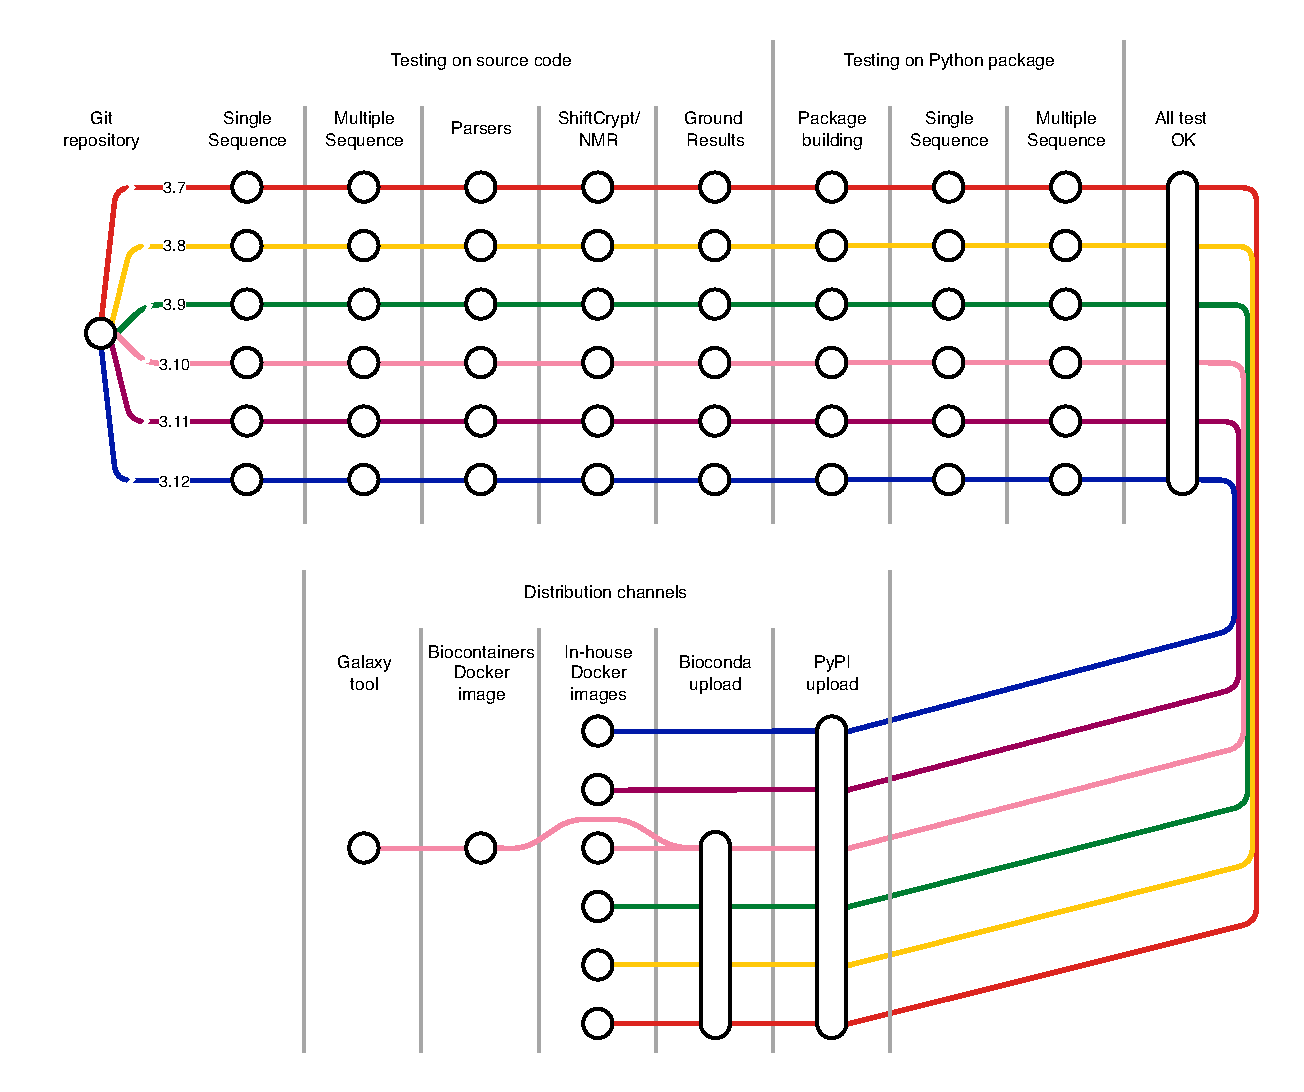
\includegraphics[width=\linewidth]{b2b_deployment/Fig/pytest_turn_bar_310.pdf}  
\centering
\caption{\textbf{Pytest process diagram.} The package testing process starts from a single Git repository, which then creates an environment per Python version from 3.7 to 3.12. For each environment, a series of tests on the source code are executed, namely the execution of single sequence, multiple sequence, parsers, and ShiftCrypt/NMR modules. Then the outputs get compared to ground results values and assessed for differences beyond float point errors (sum of absolute differences across all predicted metrics and residues, proteins and residues smaller than 0.001). A python package is then created and single sequence and multiple sequence modules are newly tested. If all tests across all Python versions are satisfactory, the python package will be uploaded to PyPI and to Bioconda. Then, an array of Docker images are created and uploaded to Docker Hub, following the settings in \supptableref{tab:docker_versions}. Finally, Bioconda automatically deposits a docker container with the Python 3.10 version of the package in Biocontainers, which can then be deployed into Galaxy.}
\label{pytest}
\end{figure*}


\endgroup

% % \chapter*{Supplementary information chapter \ref{chapter:plddt}: \\NMR-derived}
\chapter*{Supplementary information chapter 5: \\NMR-derived}
\setcounter{chapter}{5}
\addcontentsline{toc}{chapter}{Supplementary information chapter 5}
% \addcontentsline{toc}{chapter}{Supplementary information chapter \ref{chapter:plddt}}
\markright{SUPPLEMENTARY INFORMATION}

\setcounter{figure}{0} % Reset the figure counter
\renewcommand{\figurename}{Supplementary Fig.}

\setcounter{table}{0} % Reset the figure counter
\renewcommand{\tablename}{Supplementary Table}

\newpage


\begin{figure}[H]
    \centering
    \includegraphics[width=0.8\textwidth]{pLDDT/plddt_figures/box_plot_rciset_plddt_dynamine_classes.pdf}
    \caption{\textbf{pLDDT values per amino acid order classes.} The amino acids from the $S^{2}_{\text{RCI}}$ dataset were clustered in 3 classes according to their order preference: preferentially ordered (cysteine, phenylalanine, isoleucine, leucine, valine, tryptophan \& tyrosine; N=106,363), neutral (alanine, glutamic acid, lysine, methionine, glutamine, arginine, threonine \& histidine; N=155,050) and preferentially disordered (aspartic acid, glycine, asparagine, proline \& serine; N=112,945). The distributions were tested with a Mann–Whitney U test, which resulted in p-values < 0.001 in all tests.}
    \label{fig:plddt_aa_classes_boxplot}
\end{figure}


\begin{figure}[H]
    \centering
    \includegraphics[width=\textwidth]{pLDDT/plddt_figures/barplot_plddt_regions_per_ss_type_abundance_only_normalised_af_stride_af_ss_nmr_strideCons.pdf}
    \caption{\textbf{Abundance of secondary structures by pLDDT ranges.} A) The STRIDE secondary structure assignment from the structure that AlphaFold2 produces. B) The STRIDE consensus secondary structure assignment here provided is the most abundantly assigned secondary structure in the ensemble of NMR structures available. The STRIDE consensus assignment (panel B) produces a decrease in abundance for helix (H) and sheet (E) fractions as the pLDDT decreases, as well as an increase in coil (C) and turn (T) conformations. These tendencies are maintained for AlphaFold2's single structure assignment (panel A) in sheet and coil fractions, but not for helix and turn.}
    \label{fig:ss_barplots_normalised}
\end{figure}




\begin{figure}[H]
    \centering
    \includegraphics[width=0.85\textwidth]{pLDDT/plddt_figures/plddt_vs_d2d_hexbin_hist_undivided.pdf}
    \caption{\textbf{Comparison of pLDDT and $\delta 2D$ populations.} Caption in next page. 
    % For all available residues in the $S^{2}_{\text{RCI}}$ dataset, the populations of conformational states were calculated with $\delta$2D method. High populations values of a conformation indicate high presence of such conformation in the ensemble, and vice-versa. A-D: For both Helix and Sheet conformations, higher $\delta$2D populations are obtained for residues featuring high pLDDT  (\( \geq 80 \), N=62,014), gradually adopting lower populations for mid (\( 80 > \text{pLDDT} \geq 60 \), N=8,539) and low (\( < 60 \), N=4,773) pLDDT values. E-H: Coil and PPII populations are prominently higher for higher for low pLDDT ranges than for mid and high ranges. 
    % Mann-Whitney two-sided U tests p-values between each pLDDT-stratified distribution for each $\delta 2D$ conformation confirmed difference at p-values < 0.001 (table \ref{table:mann_whitney_results_delta2d}).
    }
    \label{fig:plddt_vs_d2d_undivided}
\end{figure}

\begin{figure}[H]
  \ContinuedFloat
  \caption[]{(Continuation) For all available residues in the $S^{2}_{\text{RCI}}$ dataset, the populations of conformational states were calculated with $\delta$2D method. High populations values of a conformation indicate high presence of such conformation in the ensemble, and vice-versa. A-D: For both Helix and Sheet conformations, higher $\delta$2D populations are obtained for residues featuring high pLDDT  (\( \geq 80 \), N=62,014), gradually adopting lower populations for mid (\( 80 > \text{pLDDT} \geq 60 \), N=8,539) and low (\( < 60 \), N=4,773) pLDDT values. E-H: Coil and PPII populations are prominently higher for higher for low pLDDT ranges than for mid and high ranges. 
    Mann-Whitney two-sided U tests p-values between each pLDDT-stratified distribution for each $\delta 2D$ conformation confirmed difference at p-values < 0.001 (\supptableref{table:mann_whitney_results_delta2d}).}
\end{figure}


\begin{figure}[H]
    \centering
    \includegraphics[width=0.8\textwidth]{pLDDT/plddt_figures/plddt_vs_conformational_state_propensities_hexbin_complete_hist.pdf}
    \caption{
    \textbf{Comparison between AlphaFold2 pLDDT and Constava's conformational state propensities.} Caption in next page. 
    % The pLDDT of each residue was plotted against the propensity for each of the 6 conformational states calculated in Constava. Any propensity below 0.05 was deemed non-informative and discarded to facilitate interpretation. 
    % All residues in the MD dataset were stratified in  high (N=9,523), mid (N=1,038) and low (N=809) AlphaFold2 ranges. 
    % A \& B) Hexagonal binning of AlphaFold3 C-$\alpha$ pLDDT vs Core Helix propensity and its associated pLDDT-stratified distributions. 
    % C \& D) Hexagonal binning of AlphaFold3 C-$\alpha$ pLDDT vs Surrounding Helix propensity and its associated pLDDT-stratified distributions. 
    % E \& F) Hexagonal binning of AlphaFold3 C-$\alpha$ pLDDT vs Core Sheet propensity and its associated pLDDT-stratified distributions. 
    % G \& H) Hexagonal binning of AlphaFold3 C-$\alpha$ pLDDT vs Surrounding Sheet propensity and its associated pLDDT-stratified distributions. 
    % I \& J) Hexagonal binning of AlphaFold3 C-$\alpha$ pLDDT vs Turn propensity and its associated pLDDT-stratified distributions. 
    % K \& L) Hexagonal binning of AlphaFold3 C-$\alpha$ pLDDT vs Other propensity and its associated pLDDT-stratified distributions. 
    % The p-values for the Mann-Whitney two-sided U tests between each pLDDT-stratified distribution for every conformational state can be found in supplementary table \ref{table:mann_whitney_results_md}.
    }
\label{fig:plddt_vs_constava_propensities}
\end{figure}

\begin{figure}[H]
  \ContinuedFloat
  \caption[]{ (Continuation) The pLDDT of each residue was plotted against the propensity for each of the 6 conformational states calculated in Constava. Any propensity below 0.05 was deemed non-informative and discarded to facilitate interpretation. 
    All residues in the MD dataset were stratified in  high (N=9,523), mid (N=1,038) and low (N=809) AlphaFold2 ranges. 
    A \& B) Hexagonal binning of AlphaFold3 C-$\alpha$ pLDDT vs Core Helix propensity and its associated pLDDT-stratified distributions. 
    C \& D) Hexagonal binning of AlphaFold3 C-$\alpha$ pLDDT vs Surrounding Helix propensity and its associated pLDDT-stratified distributions. 
    E \& F) Hexagonal binning of AlphaFold3 C-$\alpha$ pLDDT vs Core Sheet propensity and its associated pLDDT-stratified distributions. 
    G \& H) Hexagonal binning of AlphaFold3 C-$\alpha$ pLDDT vs Surrounding Sheet propensity and its associated pLDDT-stratified distributions. 
    I \& J) Hexagonal binning of AlphaFold3 C-$\alpha$ pLDDT vs Turn propensity and its associated pLDDT-stratified distributions. 
    K \& L) Hexagonal binning of AlphaFold3 C-$\alpha$ pLDDT vs Other propensity and its associated pLDDT-stratified distributions. 
    The p-values for the Mann-Whitney two-sided U tests between each pLDDT-stratified distribution for every conformational state can be found in \supptableref{table:mann_whitney_results_md}.}
\end{figure}

\newpage

\begin{figure}[H]
    \centering
    \includegraphics[width=\textwidth]{pLDDT/plddt_figures/plddt_vs_solvent_accessibility_hexbin_hist_undivided.pdf}
    \caption{\textbf{Comparison of pLDDT and solvent accessibility.}
    A) The AlphaFold2 pLDDT in the $S^{2}_{RCI}$ dataset were plotted against the solvent accessibility score for every residue with available values, in an hexagonal binning plot.
    B) Distributions of solvent accessibility scores, stratified in high (\( \geq 80 \), N=62,319), mid (\( 80 > \text{pLDDT} \geq 60 \), N=8,708) and low (\( < 60 \), N=4,842) AlphaFold2 pLDDT values. 
    Mann-Whitney two-sided U test confirmed significant differences between all distribution pairs with a p-value \( < 0.001 \) (\supptableref{table:mann_whitney_results}).
    }
\label{fig:plddt_vs_solvent_accesibility_undivided}
\end{figure}



\begin{figure}[H]
    \centering
    \includegraphics[width=\textwidth]{pLDDT/plddt_figures/af3_plddt_vs_conformational_state_variability_hexbin_complete_hist.pdf}
    \caption{
    \textbf{AlphaFold3 C-$\alpha$ pLDDT vs. conformational state variability.} 
    A) High pLDDT values (\( \geq 80 \), N = 10,272) concentrate in areas with lower conformational state variability. Low pLDDT \( < 60 \), N = 463) usually correspond to residues with high conformational state variability. B) This tendency is more clearly observed with pLDDT-stratified distributions, which shows that low pLDDT residues correspond to residues with high conformational state variability, therefore with high potential to exist in multiple conformations, and vice-versa for high pLDDT and low variability residues. Mid pLDDT residues \( 80 > \text{pLDDT} \geq 60 \),  N = 634) exhibit an intermediate distribution. Mann-Whitney two-sided U test yielded a p-value \( < 0.001 \) between all distributions (\supptableref{table:mann_whitney_results}). The associated distributions per propensity can be found in \suppfigref{fig:af3_plddt_vs_constava_propensities}.
    }
    \label{fig:af3_plddt_vs_conf_state_undivided}
\end{figure}


\begin{figure}[H]
    \centering
    \includegraphics[width=0.83\textwidth]{pLDDT/plddt_figures/af3_plddt_vs_conformational_state_propensities_hexbin_complete_hist.pdf}
    \caption{
    \textbf{Comparison between AlphaFold3 C-$\alpha$ pLDDT and Constava's conformational state propensities.} Caption in next page.
    % The pLDDT of each residue was plotted against the propensity for each of the 6 conformational states calculated in Constava. Any propensity below 0.05 was deemed non-informative and discarded to facilitate interpretation. 
    % All residues in the MD dataset were stratified in  high (N=10,272), mid (N=634) and low (N=463) AlphaFold3 C-$\alpha$ ranges. 
    % A \& B) Hexagonal binning of AlphaFold3 C-$\alpha$ pLDDT vs Core Helix propensity and its associated pLDDT-stratified distributions. 
    % C \& D) Hexagonal binning of AlphaFold3 C-$\alpha$ pLDDT vs Surrounding Helix propensity and its associated pLDDT-stratified distributions. 
    % E \& F) Hexagonal binning of AlphaFold3 C-$\alpha$ pLDDT vs Core Sheet propensity and its associated pLDDT-stratified distributions. 
    % G \& H) Hexagonal binning of AlphaFold3 C-$\alpha$ pLDDT vs Surrounding Sheet propensity and its associated pLDDT-stratified distributions. 
    % I \& J) Hexagonal binning of AlphaFold3 C-$\alpha$ pLDDT vs Turn propensity and its associated pLDDT-stratified distributions. 
    % K \& L) Hexagonal binning of AlphaFold3 C-$\alpha$ pLDDT vs Other propensity and its associated pLDDT-stratified distributions. 
    % The p-values for the Mann-Whitney two-sided U tests between each pLDDT-stratified distribution for every conformational state can be found in supplementary table \ref{table:mann_whitney_results_md}.
    }
\label{fig:af3_plddt_vs_constava_propensities}
\end{figure}

\begin{figure}[H]
  \ContinuedFloat
  \caption[]{ (Continuation) The pLDDT of each residue was plotted against the propensity for each of the 6 conformational states calculated in Constava. Any propensity below 0.05 was deemed non-informative and discarded to facilitate interpretation. 
    All residues in the MD dataset were stratified in  high (N=10,272), mid (N=634) and low (N=463) AlphaFold3 C-$\alpha$ ranges. 
    A \& B) Hexagonal binning of AlphaFold3 C-$\alpha$ pLDDT vs Core Helix propensity and its associated pLDDT-stratified distributions. 
    C \& D) Hexagonal binning of AlphaFold3 C-$\alpha$ pLDDT vs Surrounding Helix propensity and its associated pLDDT-stratified distributions. 
    E \& F) Hexagonal binning of AlphaFold3 C-$\alpha$ pLDDT vs Core Sheet propensity and its associated pLDDT-stratified distributions. 
    G \& H) Hexagonal binning of AlphaFold3 C-$\alpha$ pLDDT vs Surrounding Sheet propensity and its associated pLDDT-stratified distributions. 
    I \& J) Hexagonal binning of AlphaFold3 C-$\alpha$ pLDDT vs Turn propensity and its associated pLDDT-stratified distributions. 
    K \& L) Hexagonal binning of AlphaFold3 C-$\alpha$ pLDDT vs Other propensity and its associated pLDDT-stratified distributions. 
    The p-values for the Mann-Whitney two-sided U tests between each pLDDT-stratified distribution for every conformational state can be found in \supptableref{table:mann_whitney_results_md}.}
\end{figure}


\begin{figure}[H]
    \centering
    \includegraphics[width=\textwidth]{pLDDT/plddt_figures/s2_vs_plddt_af3_hexbin_undivided_hist.pdf}
    \caption{\textbf{Comparison between AlphaFold3 C-$\alpha$ pLDDT and \(S^{2}\).} Most residues in this dataset exhibit high pLDDT and high \(S^{2}\) values, represented by warmer hues in panel A. Due to the limited and uneven residues sample sizes (high pLDDT, \( \geq 80 \), N = 4,125; mid pLDDT, \( 80 > \text{pLDDT} \geq 60 \),  N = 287; low pLDDT, \( < 60 \), N = 70), it is challenging to make definitive conclusions about the sparsely populated mid and low pLDDT regions. Panel B illustrates the distributions of \(S^{2}\) values of each pLDDT range, for which Mann-Whitney two-sided U test yielded a p-value \( < 0.001 \) between all distributions (\supptableref{table:mann_whitney_results}).}

    \label{fig:af3_plddt_vs_s2_undivided}
\end{figure}

\begin{figure}[H]
    \centering
    \includegraphics[width=\textwidth]{pLDDT/plddt_figures/all_switchers_ss_af_stride_consensus_af_stride_af_ss_nmr_strideCons.pdf}
        \caption{\textbf{Distribution of STRIDE fold assignment matches and mismatches between AlphaFold2 structures and consensus NMR ensemble assignments, for diverse metrics.} Those residues in the \(S^{2}_{RCI}\) dataset with STRIDE consensus were stratified according to their secondary assignment pairs, derived from AlphaFold2 structures and the NMR models consensus assignment. A, D \& G) pLDDT distributions for residues whose consensus STRIDE assignment from NMR ensembles and from AlphaFold2 models match or mismatch. B, E \& H) \(S^{2}_{RCI}\) distributions for residues whose consensus STRIDE assignment from NMR ensembles and from AlphaFold2 models match or mismatch. C, F \& I) shiftCrypt distributions for residues whose consensus STRIDE assignment from NMR ensembles and from AlphaFold2 models match or mismatch.}
    \label{fig:af2_nmr_fold_missmatch}
\end{figure}


\begin{figure}[H]
    \centering
    \includegraphics[width=\textwidth]{pLDDT/plddt_figures/with_and_without_unique_nmr_strideCons_stratified.pdf}
    \caption{\textbf{Distribution of residues with  NMR consensus STRIDE assignment with and without unique STRIDE assignment, for diverse metrics.} Those residues in the \(S^{2}_{RCI}\) dataset with STRIDE consensus were stratified according to whether they featured a unique STRIDE assignment across all the models in their corresponding NMR ensemble. A, D, G \& J) pLDDT distributions for $\alpha$-helix, coil, turn and $\beta$-sheet respectively. B, E, H \& K) \(S^{2}_{RCI}\) distributions for $\alpha$-helix, coil, turn and $\beta$-sheet respectively. C, F, I \& L) shiftCrypt distributions for $\alpha$-helix, coil, turn and $\beta$-sheet respectively.}

    \label{fig:unique_and_or_cons}
\end{figure}

\begin{figure}[H]
    \centering
    \includegraphics[width=\textwidth]{pLDDT/plddt_figures/with_and_without_unique_nmr_strideCons_stratified_match_mismatch.pdf}
    \caption{\textbf{Distribution of residues with  NMR consensus STRIDE assignment with and without unique STRIDE assignment, with matching and mismatching NMR and AlphaFold2 fold assignments, for diverse metrics.} Those residues in the \(S^{2}_{RCI}\) dataset with STRIDE consensus were stratified according to whether they featured a unique STRIDE assignment across all the models in their corresponding NMR ensemble. Then, they were further stratified on whether or not their NMR consensus STRIDE assignment matched the AlphaFold2 STRIDE assignment. A, D, G \& J) pLDDT distributions for $\alpha$-helix, coil, turn and $\beta$-sheet respectively. B, E, H \& K) \(S^{2}_{RCI}\) distributions for $\alpha$-helix, coil, turn and $\beta$-sheet respectively. C, F, I \& L) shiftCrypt distributions for $\alpha$-helix, coil, turn and $\beta$-sheet respectively.}

    \label{fig:unique_and_or_cons_match_af2}
\end{figure}

\begin{table}[H]
	\centering
 \footnotesize
 \caption{\textbf{Results of the Mann-Whitney two-sided U tests between pLDDT-stratified subsets per Constava's conformational states on the MD dataset.} For each of Constava's conformational states, the pLDDT-stratified subsets were tested against each other with a Mann-Whitney two-sided U test to assess differential distributions.}
\begin{tabular}{@{}ccccr@{}}
\toprule
\begin{tabular}[c]{@{}c@{}}Conformational\\ state\end{tabular} &
  \begin{tabular}[c]{@{}c@{}}AlphaFold\\ version\end{tabular} &
  \begin{tabular}[c]{@{}c@{}}pLDDT\\ ranges\end{tabular} &
  \begin{tabular}[c]{@{}c@{}}Difference \\ between means\end{tabular} &
  \multicolumn{1}{c}{p-value} \\ \midrule
Core Helix  & 2 & High-Mid & 0.2161  & 6.67 x 10\(^{\text{-34}}\)  \\
Core Helix  & 2 & High-Low & 0.3427  & 2.52 x 10\(^{\text{-31}}\)  \\
Core Helix  & 2 & Mid-Low  & 0.1266  & 1.53 x 10\(^{\text{-5}}\)   \\ 
\arrayrulecolor[gray]{0.8}\hline
Surr. Helix & 2 & High-Mid & 0.0264  & 0.01955                   \\
Surr. Helix & 2 & High-Low & 0.1168  & 5.17 x 10\(^{\text{-43}}\)  \\
Surr. Helix & 2 & Mid-Low  & 0.0903  & 1.24 x 10\(^{\text{-20}}\)  \\
\arrayrulecolor[gray]{0.8}\hline
Core Sheet  & 2 & High-Mid & 0.2254  & 1.60 x 10\(^{\text{-60}}\)  \\
Core Sheet  & 2 & High-Low & 0.3074  & 2.12 x 10\(^{\text{-104}}\) \\
Core Sheet  & 2 & Mid-Low  & 0.0821  & 1.58 x 10\(^{\text{-5}}\)   \\
\arrayrulecolor[gray]{0.8}\hline
Surr. Sheet & 2 & High-Mid & 0.0339  & 1.96 x 10\(^{\text{-8}}\)   \\
Surr. Sheet & 2 & High-Low & 0.0455  & 3.02 x 10\(^{\text{-15}}\)  \\
Surr. Sheet & 2 & Mid-Low  & 0.0117  & 0.08711                   \\
\arrayrulecolor[gray]{0.8}\hline
Turn        & 2 & High-Mid & 0.0394  & 0.44796                   \\
Turn        & 2 & High-Low & 0.0826  & 0.22141                   \\
Turn        & 2 & Mid-Low  & 0.0432  & 0.45743                   \\
\arrayrulecolor[gray]{0.8}\hline
Other       & 2 & High-Mid & 0.0082  & 0.28323                   \\
Other       & 2 & High-Low & -0.0397 & 6.19 x 10\(^{\text{-15}}\)  \\
Other       & 2 & Mid-Low  & -0.0479 & 1.85 x 10\(^{\text{-9}}\)   \\
\arrayrulecolor[gray]{0.8}\hline
Core Helix  & 3 & High-Mid & 0.1990  & 4.07 x 10\(^{\text{-14}}\)  \\
Core Helix  & 3 & High-Low & 0.3498  & 4.63 x 10\(^{\text{-20}}\)  \\
Core Helix  & 3 & Mid-Low  & 0.1507  & 1.85 x 10\(^{\text{-4}}\)   \\
\arrayrulecolor[gray]{0.8}\hline
Surr. Helix & 3 & High-Mid & 0.0861  & 6.18 x 10\(^{\text{-18}}\)  \\
Surr. Helix & 3 & High-Low & 0.1203  & 7.55 x 10\(^{\text{-27}}\)  \\
Surr. Helix & 3 & Mid-Low  & 0.0343  & 0.00256                   \\
\arrayrulecolor[gray]{0.8}\hline
Core Sheet  & 3 & High-Mid & 0.2657  & 1.94 x 10\(^{\text{-58}}\)  \\
Core Sheet  & 3 & High-Low & 0.3019  & 6.68 x 10\(^{\text{-64}}\)  \\
Core Sheet  & 3 & Mid-Low  & 0.0362  & 0.29869                   \\
\arrayrulecolor[gray]{0.8}\hline
Surr. Sheet & 3 & High-Mid & 0.0423  & 6.90 x 10\(^{\text{-10}}\)  \\
Surr. Sheet & 3 & High-Low & 0.0462  & 1.51 x 10\(^{\text{-10}}\)  \\
Surr. Sheet & 3 & Mid-Low  & 0.0039  & 0.66095                   \\
\arrayrulecolor[gray]{0.8}\hline
Turn        & 3 & High-Mid & 0.0628  & 0.48281                   \\
Turn        & 3 & High-Low & 0.0779  & 0.13434                   \\
Turn        & 3 & Mid-Low  & 0.0152  & 0.33197                   \\
\arrayrulecolor[gray]{0.8}\hline
Other       & 3 & High-Mid & -0.0178 & 0.000078                  \\
Other       & 3 & High-Low & -0.0288 & 2.72 x 10\(^{\text{-8}}\)   \\
Other       & 3 & Mid-Low  & -0.0110 & 0.15908                   \\ \arrayrulecolor{black} \bottomrule
\end{tabular}
	\label{table:mann_whitney_results_md}
\end{table}

\begin{table}[H]
\centering
\small
\caption{\textbf{Results of the Mann-Whitney two-sided U tests between pLDDT-stratified subsets for $S^{2}_{RCI}$ $\delta 2D$ conformations in AlphaFold2.} For each conformation type, the pLDDT-stratified subsets were tested against each other with a Mann-Whitney two-sided U test to assess differential distributions. \textit{Note: p-values marked with * were too low for Scipy to differentiate from 0.}}
\begin{tabular}{@{}cccr@{}}
\toprule
Conformation & \begin{tabular}[c]{@{}c@{}}pLDDT\\ ranges\end{tabular} & \begin{tabular}[c]{@{}c@{}}Difference\\ between means\end{tabular} & \multicolumn{1}{c}{p-value} \\ \midrule
$\delta 2D$ Helix & High-Mid & 0.1185  & 3.38 x 10\(^{\text{-55}}\)  \\
$\delta 2D$ Helix & High-Low & 0.2896  & 0.0*                      \\
$\delta 2D$ Helix & Mid-Low  & 0.1711  & 1.23 x 10\(^{\text{-300}}\) \\
\arrayrulecolor[gray]{0.8}\hline
$\delta 2D$ Sheet & High-Mid & 0.1181  & 5.03 x 10\(^{\text{-49}}\)  \\
$\delta 2D$ Sheet & High-Low & 0.1723  & 5.44 x 10\(^{\text{-53}}\)  \\
$\delta 2D$ Sheet & Mid-Low  & 0.0542  & 2.63 x 10\(^{\text{-7}}\)   \\
\arrayrulecolor[gray]{0.8}\hline
$\delta 2D$ Coil  & High-Mid & -0.1775 & 0.0*                      \\
$\delta 2D$ Coil  & High-Low & -0.3184 & 0.0*                      \\
$\delta 2D$ Coil  & Mid-Low  & -0.1410 & 3.76 x 10\(^{\text{-305}}\) \\
\arrayrulecolor[gray]{0.8}\hline
$\delta 2D$ PPII  & High-Mid & -0.0592 & 0.0*                      \\
$\delta 2D$ PPII  & High-Low & -0.1435 & 0.0*                      \\
$\delta 2D$ PPII  & Mid-Low  & -0.0843 & 0.0*                      \\ \arrayrulecolor{black} \bottomrule
\end{tabular}

\label{table:mann_whitney_results_delta2d}
\end{table}


\begin{table}[H]
\centering
\small
\caption{\textbf{Results of the Mann-Whitney two-sided U tests between pLDDT-stratified subsets.} For each dataset, the pLDDT-stratified subsets were tested against each other with a Mann-Whitney two-sided U test to assess differential distributions. \textit{Note: p-values marked with * were too low for Scipy to differentiate from 0.}}
\begin{tabular}{@{}cccccr@{}}
\toprule
Dataset &
  Metric &
  \begin{tabular}[c]{@{}c@{}}AlphaFold\\ version\end{tabular} &
  \begin{tabular}[c]{@{}c@{}}pLDDT\\ ranges\end{tabular} &
  \begin{tabular}[c]{@{}c@{}}Difference\\ between \\means\end{tabular} &
  \multicolumn{1}{c}{p-value} \\ \midrule
\(S^{2}_{\text{RCI}}\) & \(S^{2}_{\text{RCI}}\)  & 2 & high-mid & 0.1417  & 0*                        \\
\(S^{2}_{\text{RCI}}\) & \(S^{2}_{\text{RCI}}\)  & 2 & high-low & 0.4150  & 0*                        \\
\(S^{2}_{\text{RCI}}\) & \(S^{2}_{\text{RCI}}\)  & 2 & mid-low  & 0.2732  & 0*                        \\ \arrayrulecolor[gray]{0.8}\hline
\(S^{2}_{\text{RCI}}\) & ShiftCrypt            & 2 & high-mid & 0.0152  & 0.002                     \\
\(S^{2}_{\text{RCI}}\) & ShiftCrypt            & 2 & high-low & -0.0201 & 4.55 x 10\(^{\text{-7}}\)   \\
\(S^{2}_{\text{RCI}}\) & ShiftCrypt            & 2 & mid-low  & -0.0353 & 9.45 x 10\(^{\text{-21}}\)  \\ \arrayrulecolor[gray]{0.8}\hline
\(S^{2}_{\text{RCI}}\) & \begin{tabular}[c]{@{}c@{}}Solvent\\accessibility\end{tabular} & 2 & high-mid & -0.1851 & 0*                        \\
\(S^{2}_{\text{RCI}}\) & \begin{tabular}[c]{@{}c@{}}Solvent\\accessibility\end{tabular} & 2 & high-low & -0.3521 & 0*                        \\
\(S^{2}_{\text{RCI}}\) & \begin{tabular}[c]{@{}c@{}}Solvent\\accessibility\end{tabular} & 2 & mid-low  & -0.1670 & 1.93 x 10\(^{\text{-297}}\) \\ \arrayrulecolor[gray]{0.8}\hline
\(S^{2}\)            & \(S^{2}\)             & 2 & high-mid & 0.1352  & 5.60 x 10\(^{\text{-24}}\)  \\
\(S^{2}\)            & \(S^{2}\)             & 2 & high-low & 0.4238  & 1.19 x 10\(^{\text{-53}}\)  \\
\(S^{2}\)            & \(S^{2}\)             & 2 & mid-low  & 0.2886  & 2.12 x 10\(^{\text{-19}}\)  \\ \arrayrulecolor[gray]{0.8}\hline
\(S^{2}\)            & \(S^{2}\)             & 3 & high-mid & 0.1681  & 1.74 x 10\(^{\text{-43}}\)  \\
\(S^{2}\)            & \(S^{2}\)             & 3 & high-low & 0.4904  & 6.36 x 10\(^{\text{-38}}\)  \\
\(S^{2}\)            & \(S^{2}\)             & 3 & mid-low  & 0.3223  & 2.45 x 10\(^{\text{-16}}\)  \\ \arrayrulecolor[gray]{0.8}\hline
MD                   & Conf. state var.      & 2 & high-mid & -0.1468 & 3.46 x 10\(^{\text{-143}}\) \\
MD                   & Conf. state var.      & 2 & high-low & -0.2197 & 1.23 x 10\(^{\text{-246}}\) \\
MD                   & Conf. state var.      & 2 & mid-low  & -0.0729 & 1.48 x 10\(^{\text{-22}}\)  \\ \arrayrulecolor[gray]{0.8}\hline
MD                   & Conf. state var.      & 3 & high-mid & -0.1743 & 1.46 x 10\(^{\text{-126}}\) \\
MD                   & Conf. state var.      & 3 & high-low & -0.2258 & 4.6 x 10\(^{\text{-155}}\)  \\
MD                   & Conf. state var.      & 3 & mid-low  & -0.0515 & 2.08 x 10\(^{\text{-7}}\)   \\ \arrayrulecolor{black} \bottomrule
\end{tabular}

\label{table:mann_whitney_results}
\end{table}




% % \chapter*{Supplementary information chapter \ref{chapter:plddt}: \\NMA-derived}
\chapter*{Supplementary information chapter 6: \\NMA-derived}


\newpage

On the $S_{\text{RCI}}^{2}$ dataset of 762 proteins, WEBnma was carried out on the 762 AlphaFold2 models. Therefore, based on WEBnma output, the final dataset consists of 762 AlphaFold2 models. The predicted RMSF values of each coil residue in all 762 proteins are shown in (\suppfigref{fig:plddt_sup:sup12}). The supplementary figure shows some extreme RMSF values in Flexible-pLDDT regions. As explained in the main text, these extreme values can originate artificially from loosely packed stretches in the protein structure. We have therefore adapted the RMSF analysis to reduce the artificial RMSF outliers. As shown in the folFlexibleing (section Truncation criterion), the N- and C-terminal tails from AlphaFold2 models were truncated. The truncation criterion is based on the number of C$\alpha$ contacts. The final number of truncated proteins in the dataset was 755, and the remaining 7 did not require cutting of termini. Subsequently, normal mode analysis with WEBnma was again performed on these 755 truncated models, and the RMSF was recomputed. The RMSF results are shown for 762 proteins, including both the 755 truncated models and the 7 models that did not require termini cutting (referred to as truncated $S_{\text{RCI}}^{2}$ dataset). Apart from (\suppfigref{fig:plddt_sup:sup12}, \suppfigref{fig:plddt_sup:sup13}, and \supptableref{tab:plddt_sup:suptable4}) all figures and data in the main document and SI contain the RMSF of truncated $S_{\text{RCI}}^{2}$ dataset. \suppfigref{fig:plddt_sup:sup13} shows the effect of the truncation by comparing the RMSF before truncation and the RMSF after truncation.
\newpage

\begin{figure}[H]
    \centering
    \includegraphics[width=0.75\linewidth]{pLDDT//plddt_figures//supplementary_bhawna/supfig12.pdf}
\caption{\textbf{Comparison of pLDDT and RMSF in coils.} pLDDT vs RMSF of 762 proteins for coil residues before truncation. The colour bar represents the Gaussian kernel density estimate of the dataset. The red vertical lines divide the dataset into Rigid pLDDT ($\geq 80$), Ambiguous ($60 \leq \text{pLDDT} < 80$) and Flexible ($< 60$) pLDDT regions.}
    \label{fig:plddt_sup:sup12}
\end{figure}


\begin{figure}[H]
    \centering
    \includegraphics[width=\linewidth]{pLDDT//plddt_figures//supplementary_bhawna/supfig13.pdf}
    \caption{\textbf{Comparison of pLDDT and RMSF in coils.} RMSF vs pLDDT of amino acid residues exhibiting coils in non-truncated (A, C, E) and truncated (B, D, F) AlphaFold2 structures in Flexible-pLDDT (A, B), Ambiguous-pLDDT (C, D), and c) Rigid-pLDDT (E, F) regions. Only the amino acids that are present in both the non-truncated and truncated AlphaFold2 models are included.}
    \label{fig:plddt_sup:sup13}
\end{figure}

% S Table 4

\begin{table}[H]
\small
\centering
\caption{\textbf{RMSF values of are grouped according to pLDDT in Flexible-pLDDT, Ambiguous-pLDDT and Rigid-pLDDT for AlphaFold2 models before truncation.} The table reports the minimum, maximum, mean, and standard deviation for each group.}
\label{tab:plddt_sup:suptable4}
\begin{tabular}{@{}cccccc@{}}
\toprule
\begin{tabular}[c]{@{}c@{}}Secondary\\ structure\end{tabular} & pLDDT range & min & max & mean & std \\ \midrule
Coil           & Flexible  & 0.22  & 184.99 & 6.28 & 5.83 \\
Strand         & Flexible  & 33.97 & 1.58   & 1.84 & 1.66 \\
$\alpha$-Helix & Flexible  & 29.67 & 1.35   & 1.49 & 2.15 \\
Turn           & Flexible  & 24.68 & 1.57   & 1.87 & 2.74 \\
310-Helix      & Flexible  & 32.52 & 1.63   & 1.91 & 3.29 \\
Bridge         & Flexible  & 30.04 & 1.37   & 1.55 & 2.50 \\
\arrayrulecolor[gray]{0.8}\hline
Coil           & Ambiguous  & 29.29 & 1.48   & 1.78 & 5.16 \\
Strand         & Ambiguous  & 0.23  & 21.63  & 1.49 & 1.6  \\
$\alpha$-Helix & Ambiguous  & 0.18  & 23.61  & 2.02 & 2.37 \\
Turn           & Ambiguous  & 0.20  & 33.05  & 2.04 & 2.56 \\
310-Helix      & Ambiguous  & 0.21  & 27.39  & 2.11 & 3.07 \\
Bridge         & Ambiguous  & 0.26  & 13.06  & 1.66 & 2.04 \\
\arrayrulecolor[gray]{0.8}\hline
Coil           & Rigid & 0.15  & 33.97  & 1.58 & 1.84 \\
Strand         & Rigid & 0.15  & 29.67  & 1.35 & 1.49 \\
$\alpha$-Helix & Rigid & 0.14  & 24.68  & 1.57 & 1.87 \\
Turn           & Rigid & 0.15  & 32.52  & 1.63 & 1.91 \\
310-Helix      & Rigid & 0.20  & 30.04  & 1.37 & 1.55 \\
Bridge         & Rigid & 0.15  & 29.29  & 1.48 & 1.78 \\ \bottomrule
\end{tabular}
\end{table}



\subsection*{Truncation criterion}\label{section:supNMA:truncation}

For determining N- and/or C-termini truncation, the C$\alpha$ contacts were assessed within a 10 Å (1 nm) cut-off for each protein in the dataset. In proteins, helices and strands consistently exhibited significant contacts, surpassing approximately 13 contacts per residue across the dataset with Flexibleer RMSF ($<20$ Å) as shown in (\suppfigref{fig:plddt_sup:sup14}). An example is shown in \suppfigref{fig:plddt_sup:sup15}. In contrast, coils showed fewer than 13 contacts per residue and showed very Rigid RMSF ($>50$ Å). Thus, a 13-contact cutoff was selected to truncate the termini.
FolFlexibleing this criterion, all first residues with fewer than 13 contacts were cut both in the N-terminal and C-terminal. Consequently, if the first residue of an N- or C-terminal has $\geq 13$ contacts, this terminal was not truncated. Only the termini were truncated, so an accidental Flexible contact region in the core of the protein would not get cut.


\begin{figure}[H]
    \centering
    \includegraphics[width=\linewidth]{pLDDT//plddt_figures//supplementary_bhawna/supfig14.pdf}
    \caption{Mean number of contacts Mean number of C$\alpha$ contacts within a 10 Å cut-off for first 30 residues depicting N-terminal (A) and last 30 residues depicting C-terminal (B) averaged over all 762 proteins. The black line represents the mean contacts, with the standard deviation shown as grey shaded area.}
    \label{fig:plddt_sup:sup14}
\end{figure}

\begin{figure}[H]
    \centering
    \includegraphics[width=\linewidth]{pLDDT//plddt_figures//supplementary_bhawna/supfig15.pdf}
    \caption{\textbf{Number of C$\alpha$ contacts profile.} (A) and RMSF profile (B) of Q92688. The red dashed line in A represents the contact cut-off (13 contacts) and red dashed line in B represents the RMSF at contact cut-off. The 3D structure of Q92688 is shown in C with a red Rigidlighted region for truncation.}
    \label{fig:plddt_sup:sup15}
\end{figure}

\subsection*{Additional analysis of RMSF and correlation with pLDDT or $S_{\text{RCI}}^{2}$}

The RMSF values for the dataset with truncated dataset are further analysed (now 762 proteins) according to their secondary structure element as predicted by STRIDE.

The six considered secondary structure elements are coil, strand, $\alpha$-helix, turn, 310-helix, and bridge. The tables report the minimum, maximum, mean, and standard deviation for the RMSF values in each secondary structure group. \supptableref{tab:plddt_sup:suptable5} gives three columns according to the pLDDT value as given by AlphaFold2: Flexible-pLDDT, Ambiguous-pLDDT, and Rigid-pLDDT. \supptableref{tab:plddt_sup:suptable6} gives three columns according to the $S_{\text{RCI}}^{2}$ value as included in the truncated $S_{\text{RCI}}^{2}$ dataset: flexible, ambiguous, and rigid.

Next, the Pearson correlation coefficient between the RMSF values and the pLDDT values were computed in each group (Flexible-pLDDT, Ambiguous-pLDDT, and Rigid-pLDDT) in (\supptableref{tab:plddt_sup:suptable7}). Moreover, the Pearson correlation coefficient between RMSF and pLDDT was computed, without considering the subgroups of pLDDT (\supptableref{tab:plddt_sup:suptable7}). Similarly, the Pearson correlation coefficient between RMSF and $S_{\text{RCI}}^{2}$ was computed for each group (flexible, ambiguous, and rigid), and without considering subgroups of $S_{\text{RCI}}^{2}$ (\supptableref{tab:plddt_sup:suptable8}). For both RMSF and pLDDT, RMSF and $S_{\text{RCI}}^{2}$, the Pearson correlation was calculated for each secondary structure group, and without the classification of secondary structure.
Next, The Pearson correlation coefficient between the RMSF values and $S_{\text{RCI}}^{2}$ can also be computed for each individual AlphaFold2 and NMR model in the truncated $S_{\text{RCI}}^{2}$ dataset. This is reported as a histogram in \suppfigref{fig:plddt_sup:sup18} (blue) using the RMSF values of the 746 AlphaFold2 models and \suppfigref{fig:plddt_sup:sup18} (yellow) using the RMSF values of 14,069 NMR models (as explained in the results section 6.3.5.2).
% \ref{section:plddt:s2_nma_nmr}).

\begin{figure}[H]
    \centering
    \includegraphics[width=\linewidth]{pLDDT//plddt_figures//supplementary_bhawna/supfig16.pdf}
    \caption{\textbf{Comparison of pLDDT and RMSF.} RMSF values versus pLDDT value of each amino acid, visualised with a Gaussian kernel estimator for $S_{\text{RCI}}^{2}$ data set. One subplot for each secondary structure element: A) coil (N = 105,172), B) strand (N = 54,786), C) $\alpha$-helix (N = 109,639), D) turn (N = 58,328), E) 310-helix (N = 7,931), and F) bridge (N = 2,445), where N represents number of amino acid residues. The red vertical lines divide the dataset into Rigid pLDDT ($\geq 80$), Ambiguous ($60 \leq \text{pLDDT} < 80$) and Flexible ($< 60$) pLDDT regions.}
    \label{fig:plddt_sup:sup16}
\end{figure}

% S Table 5

\begin{table}[H]
\small
\centering
\caption{\textbf{RMSF values are grouped according to pLDDT in Flexible-pLDDT, Ambiguous-pLDDT and Rigid-pLDDT.} The table reports the minimum, maximum, mean, and standard deviation for each group.}
\label{tab:plddt_sup:suptable5}
\begin{tabular}{@{}cccccc@{}}
\toprule
\begin{tabular}[c]{@{}c@{}}Secondary\\ structure\end{tabular} & pLDDT range & min & max & mean & std \\ \midrule
Coil           & Low  & 0.22 & 49.24 & 5.65 & 4.43 \\
Strand         & Low  & 0.24 & 8.82  & 1.89 & 1.86 \\
$\alpha$-Helix & Low  & 0.25 & 27.35 & 1.87 & 1.83 \\
Turn           & Low  & 0.20 & 32.16 & 2.16 & 2.03 \\
310-Helix      & Low  & 0.25 & 27.95 & 2.08 & 3.19 \\
Bridge         & Low  & 0.22 & 22.78 & 1.89 & 3.00 \\
\arrayrulecolor[gray]{0.8}\hline
Coil           & Mid  & 0.21 & 26.71 & 1.89 & 2.18 \\
Strand         & Mid  & 0.21 & 12.6  & 1.35 & 1.46 \\
$\alpha$-Helix & Mid  & 0.18 & 27.26 & 1.84 & 2.26 \\
Turn           & Mid  & 0.15 & 29.68 & 1.74 & 2.16 \\
310-Helix      & Mid  & 0.21 & 32.8  & 1.89 & 2.78 \\
Bridge         & Mid  & 0.26 & 13.43 & 1.34 & 1.53 \\
\arrayrulecolor[gray]{0.8}\hline
Coil           & High & 0.14 & 30.48 & 1.27 & 1.29 \\
Strand         & High & 0.14 & 20.28 & 1.11 & 1.13 \\
$\alpha$-Helix & High & 0.13 & 25.39 & 1.38 & 1.65 \\
Turn           & High & 0.13 & 20.95 & 1.33 & 1.36 \\
310-Helix      & High & 0.16 & 17.96 & 1.14 & 1.16 \\
Bridge         & High & 0.15 & 14.87 & 1.20 & 1.16 \\ \bottomrule
\end{tabular}
\end{table}

% S Table 6
\begin{table}[H]
\small
\centering
\caption{\textbf{RMSF values are grouped according to $S_{\text{RCI}}^{2}$ values in flexible (< .7), ambiguous (0.7-0.8), and rigid(> 0.8).} The table reports the maximum, maximum, mean, and standard deviation for each group.}
\label{tab:plddt_sup:suptable6}
\begin{tabular}{@{}cccccc@{}}
\toprule
\begin{tabular}[c]{@{}c@{}}Secondary\\ structure\end{tabular} & $S_{\text{RCI}}^{2}$ & min & max & mean & std \\ \midrule
Coil           & Flexible  & 0.21 & 25.06 & 2.43 & 2.60 \\
Strand         & Flexible  & 0.23 & 15.44 & 1.38 & 1.66 \\
$\alpha$-Helix & Flexible  & 0.23 & 20.99 & 2.04 & 2.06 \\
Turn           & Flexible  & 0.19 & 22.01 & 1.89 & 1.79 \\
310-Helix      & Flexible  & 0.23 & 11.44 & 1.70 & 1.94 \\
Bridge         & Flexible  & 0.29 & 9.20  & 1.52 & 1.49 \\
\arrayrulecolor[gray]{0.8}\hline
Coil           & Ambiguous  & 0.20 & 16.88 & 1.40 & 1.58 \\
Strand         & Ambiguous  & 0.20 & 15.16 & 1.28 & 1.33 \\
$\alpha$-Helix & Ambiguous  & 0.21 & 16.51 & 1.56 & 1.72 \\
Turn           & Ambiguous  & 0.20 & 17.37 & 1.52 & 1.70 \\
310-Helix      & Ambiguous  & 0.21 & 10.54 & 1.45 & 1.45 \\
Bridge         & Ambiguous  & 0.22 & 10.09 & 1.27 & 1.34 \\
\arrayrulecolor[gray]{0.8}\hline
Coil           & Rigid & 0.19 & 14.74 & 1.30 & 1.47 \\
Strand         & Rigid & 0.17 & 14.77 & 1.13 & 1.25 \\
$\alpha$-Helix & Rigid & 0.15 & 19.04 & 1.23 & 1.35 \\
Turn           & Rigid & 0.20 & 14.70 & 1.35 & 1.40 \\
310-Helix      & Rigid & 0.21 & 11.74 & 1.21 & 1.32 \\
Bridge         & Rigid & 0.21 & 14.87 & 1.37 & 1.73 \\ \bottomrule
\end{tabular}
\end{table}

\begin{figure}[H]
    \centering
    \includegraphics[width=\linewidth]{pLDDT//plddt_figures//supplementary_bhawna/supfig17.pdf}
    \caption{\textbf{Comparison of $S_{\text{RCI}}^{2}$ and RMSF.} RMSF values versus $S_{\text{RCI}}^{2}$ value of each amino acid, visualised with a Gaussian kernel estimator for truncated $S_{\text{RCI}}^{2}$ data set. One subplot for each secondary structure element: A) coil (N = 11,634), B) strand (N = 18,640), C) $\alpha$-helix (N = 25,861), D) turn (N = 14,759), E) 310-helix (N = 2,250), and F) bridge (N = 670), where N represents number of amino acid residues. The green vertical lines divide the dataset into flexible ($<0.70$), ambiguous ($0.70 - 0.80$), and rigid ($\geq 0.80$) regions.}

    \label{fig:plddt_sup:sup17}
\end{figure}

% S Table 7


\begin{table}[H]
\centering
\small
\caption{Pearson correlation coefficients and p-values are provided for RMSF and pLDDT. These correlations are analysed as well as for the full range of pLDDT, with and without the classification of secondary structure elements (all SS).}
\label{tab:plddt_sup:suptable7}
\begin{tabular}{@{}lccc@{}}
\toprule
Subset                         & Secondary Structure & \multicolumn{1}{c}{Pearson} & \multicolumn{1}{c}{p-value}  \\ \midrule
Flexible-pLDDT                      & Coil                & 0.16                        & 0.00                         \\
Ambiguous-pLDDT                      & Coil                & -0.17                       & 8.98 x 10$^{\text{-55}}$     \\
Rigid-pLDDT                     & Coil                & -0.16                       & 1.90 x 10$^{\text{-157}}$    \\
All pLDDT                      & Coil                & -0.43                       & 0.00                         \\
\arrayrulecolor[gray]{0.8}\hline
Flexible-pLDDT                      & Strand              & 0.21                        & 4.62 x 10$^{\text{-6}}$      \\
Ambiguous-pLDDT                      & Strand              & -0.01                       & 4.51 x 10$^{\text{-1}}$      \\
Rigid-pLDDT                     & Strand              & -0.12                       & 8.7 x 10$^{\text{-165}}$     \\
All pLDDT                      & Strand              & -0.12                       & 1.07 x 10$^{\text{-185}}$    \\
\arrayrulecolor[gray]{0.8}\hline
Flexible-pLDDT                      & $\alpha$-helix      & 0.16                        & 9.41 x 10$^{\text{-36}}$     \\
Ambiguous-pLDDT                      & $\alpha$-helix      & -0.04                       & 9.19 x 10$^{\text{-7}}$      \\
Rigid-pLDDT                     & $\alpha$-helix      & -0.10                       & 1.28 x 10$^{\text{-183}}$    \\
All pLDDT                      & $\alpha$-helix      & -0.11                       & 4.49 x 10$^{\text{-319}}$    \\
\arrayrulecolor[gray]{0.8}\hline
Flexible-pLDDT                      & Turn                & 0.07                        & 9.71 x 10$^{\text{-15}}$     \\
Ambiguous-pLDDT                      & Turn                & -0.04                       & 1.93 x 10$^{\text{-6}}$      \\
Rigid-pLDDT                     & Turn                & -0.16                       & 7.83 x 10$^{\text{-208}}$    \\
All pLDDT                      & Turn                & -0.20                       & 0.00                         \\
\arrayrulecolor[gray]{0.8}\hline
Flexible-pLDDT                      & 3$_{10}$-helix      & 0.13                        & 1.28 x 10$^{\text{-3}}$      \\
Ambiguous-pLDDT                      & 3$_{10}$-helix      & -0.04                       & 1.91 x 10$^{\text{-1}}$      \\
Rigid-pLDDT                     & 3$_{10}$-helix      & -0.17                       & 3.16 x 10$^{\text{-41}}$     \\
All pLDDT                      & 3$_{10}$-helix      & -0.19                       & 1.08 x 10$^{\text{-67}}$     \\
\arrayrulecolor[gray]{0.8}\hline
Flexible-pLDDT                      & Bridge              & 0.07                        & 4.99 x 10$^{\text{-1}}$      \\
Ambiguous-pLDDT                      & Bridge              & 0.00                        & 9.63 x 10$^{\text{-1}}$      \\
Rigid-pLDDT                     & Bridge              & -0.18                       & 5.08 x 10$^{\text{-17}}$     \\
All pLDDT                      & Bridge              & -0.14                       & 3.51 x 10$^{\text{-12}}$     \\
\arrayrulecolor[gray]{0.8}\hline
Flexible-pLDDT                      & All                 & -0.04                       & 1.93 x 10$^{\text{-26}}$     \\
Ambiguous-pLDDT                      & All                 & -0.07                       & 2.99 x 10$^{\text{-47}}$     \\
Rigid-pLDDT                     & All                 & -0.13                       & 0.00                         \\
All pLDDT                      & All                 & -0.24                       & 0.00                                          \\ \bottomrule
\end{tabular}
\end{table}


\begin{table}[H]
\centering
\small
\caption{Pearson correlation coefficients and p-values are provided for RMSF and $S_{\text{RCI}}^{2}$. These correlations are analysed as well as for the full range of pLDDT, with and without the classification of secondary structure elements (all SS).}
\label{tab:plddt_sup:suptable8}
\begin{tabular}{@{}lccc@{}}
\toprule
Subset                         & Secondary Structure & \multicolumn{1}{c}{Pearson} & \multicolumn{1}{c}{p-value}  \\ \midrule
Flexible $S_{\text{RCI}}^{2}$  & Coil                & -0.26                       & 3.22 x 10$^{\text{-66}}$     \\
Ambiguous $S_{\text{RCI}}^{2}$ & Coil                & -0.07                       & 7.65 x 10$^{\text{-5}}$      \\
Rigid $S_{\text{RCI}}^{2}$     & Coil                & -0.05                       & 1.27 x 10$^{\text{-3}}$      \\
All $S_{\text{RCI}}^{2}$       & Coil                & -0.32                       & 1.06 x 10$^{\text{-278}}$    \\
\arrayrulecolor[gray]{0.8}\hline
Flexible $S_{\text{RCI}}^{2}$  & Strand              & -0.11                       & 4.84 x 10$^{\text{-3}}$      \\
Ambiguous $S_{\text{RCI}}^{2}$ & Strand              & -0.04                       & 2.57 x 10$^{\text{-2}}$      \\
Rigid $S_{\text{RCI}}^{2}$     & Strand              & -0.06                       & 6.85 x 10$^{\text{-15}}$     \\
All $S_{\text{RCI}}^{2}$       & Strand              & -0.08                       & 5.2 x 10$^{\text{-26}}$      \\
\arrayrulecolor[gray]{0.8}\hline
Flexible $S_{\text{RCI}}^{2}$  & $\alpha$-helix      & -0.01                       & 5.62 x 10$^{\text{-1}}$      \\
Ambiguous $S_{\text{RCI}}^{2}$ & $\alpha$-helix      & -0.08                       & 2.07 x 10$^{\text{-4}}$      \\
Rigid $S_{\text{RCI}}^{2}$     & $\alpha$-helix      & -0.05                       & 2.66 x 10$^{\text{-14}}$     \\
All $S_{\text{RCI}}^{2}$       & $\alpha$-helix      & -0.15                       & 4.72 x 10$^{\text{-124}}$    \\
\arrayrulecolor[gray]{0.8}\hline
Flexible $S_{\text{RCI}}^{2}$  & Turn                & -0.11                       & 9.5 x 10$^{\text{-13}}$      \\
Ambiguous $S_{\text{RCI}}^{2}$ & Turn                & -0.03                       & 5.21 x 10$^{\text{-2}}$      \\
Rigid $S_{\text{RCI}}^{2}$     & Turn                & -0.03                       & 8.36 x 10$^{\text{-3}}$      \\
All $S_{\text{RCI}}^{2}$       & Turn                & -0.15                       & 1.15 x 10$^{\text{-76}}$     \\
\arrayrulecolor[gray]{0.8}\hline
Flexible $S_{\text{RCI}}^{2}$  & 3$_{10}$-helix      & -0.16                       & 1.23 x 10$^{\text{-2}}$      \\
Ambiguous $S_{\text{RCI}}^{2}$ & 3$_{10}$-helix      & -0.02                       & 7.13 x 10$^{\text{-1}}$      \\
Rigid $S_{\text{RCI}}^{2}$     & 3$_{10}$-helix      & -0.08                       & 3.34 x 10$^{\text{-3}}$      \\
All $S_{\text{RCI}}^{2}$       & 3$_{10}$-helix      & -0.14                       & 4.67 x 10$^{\text{-11}}$     \\
\arrayrulecolor[gray]{0.8}\hline
Flexible $S_{\text{RCI}}^{2}$  & Bridge              & -0.14                       & 1.34 x 10$^{\text{-1}}$      \\
Ambiguous $S_{\text{RCI}}^{2}$ & Bridge              & -0.18                       & 1.44 x 10$^{\text{-2}}$      \\
Rigid $S_{\text{RCI}}^{2}$     & Bridge              & -0.07                       & 1.91 x 10$^{\text{-1}}$      \\
All $S_{\text{RCI}}^{2}$       & Bridge              & -0.07                       & 6.56 x 10$^{\text{-2}}$      \\
\arrayrulecolor[gray]{0.8}\hline
Flexible $S_{\text{RCI}}^{\text{2}}$  & All                 & -0.17                       & 6.97 x 10$^{\text{-75}}$     \\
Ambiguous $S_{\text{RCI}}^{\text{2}}$ & All                 & -0.05                       & 4.03 x 10$^{\text{-10}}$     \\
Rigid $S_{\text{RCI}}^{\text{2}}$     & All                 & -0.06                       & 3.59 x 10$^{\text{-44}}$     \\
All $S_{\text{RCI}}^{\text{2}}$       & All                 & -0.22                       & 0.00                         \\ \bottomrule
\end{tabular}
\end{table}

\begin{figure}[H]
    \centering
    \includegraphics[width=0.75\linewidth]{pLDDT//plddt_figures//supplementary_bhawna/supfig18.pdf}
    \caption{\textbf{Pearson correlation coefficients between RMSF and $S_{\text{RCI}}^{2}$.} Distribution of Pearson correlation coefficients between RMSF values and $S_{\text{RCI}}^{2}$ values of amino acids for AlphaFold2 models (blue) and NMR models (yellow).}
    \label{fig:plddt_sup:sup18}
\end{figure}

\subsection*{Examples of $S_{\text{RCI}}^{2}$ and RMSF correlation for Alphafold2 and NMR models}

The correlation between the per-residue RMSF and per-residue $S_{\text{RCI}}^{2}$ values of a given protein is generally expected to be negative, because rigid regions would correspond to Rigid RMSF and Flexible $S_{\text{RCI}}^{2}$. There were a few NMR models that showed (unexpected) positive correlation between $S_{\text{RCI}}^{2}$ and RMSF.

\subsection*{Example of a protein where the AlphaFold2 model has a slightly weaker negative $S_{\text{RCI}}^{2}$ versus RMSF correlation than the NMR model}

The Pearson correlation coefficient between RMSF and $S_{\text{RCI}}^{2}$ values is -0.52 for the AlphaFold2 model of protein Q96LL9-2YUA (BMRB id 11144). For the 20 NMR structures, 19 have a Pearson correlation coefficient between RMSF and $S_{\text{RCI}}^{2}$ that lie in the range -0.65 to -0.81 and the remaining model shows -0.40. Therefore, the AlphaFold2 model has weaker correlation than most of the NMR models. In addition, in the figures beFlexible, the NMR model shows residues with ambiguous secondary structure (grey). The ambiguous residues were computed by the dumb consensus of secondary structure with a 70\% threshold within the NMR ensemble.

\begin{figure}[H]
    \centering
    \includegraphics[width=\linewidth]{pLDDT//plddt_figures//supplementary_bhawna/supfig19.pdf}
    \caption{\textbf{Example of a protein (Q96LL9-2YUA).} The 3D structures with secondary structure mapping colours are shown on the right: AlphaFold2 model (right top) and NMR ensemble (right bottom, 20 NMR models shown at once). Comparing $S_{\text{RCI}}^{2}$ (red, dashed) and RMSF (black line) of the AlphaFold2 model and the NMR ensemble (for this protein, there were 20 NMR models within the ensemble). The secondary structure is indicated with shaded regions. The pLDDT of the sequence is shown beFlexible the plots. (Color legends at the top of the figure.)}
    \label{fig:plddt_sup:sup19}
\end{figure}

\subsection*{Example of a protein where the AlphaFold2 model has a slightly stronger negative $S_{\text{RCI}}^{2}$ versus RMSF correlation than (most of) the NMR models}

The Pearson correlation coefficient between RMSF and $S_{\text{RCI}}^{2}$ values is -0.91 for the AlphaFold2 model of protein Q922K9-2D8J (BMRB id: 11214). For the 20 NMR models within the ensemble, the Pearson correlation coefficient between RMSF and $S_{\text{RCI}}^{2}$ lie in the range -0.63 to -0.91, where 19 models show correlation coefficient beFlexible -0.91. Therefore, the AlphaFold2 model has stronger negative correlation than most of the NMR models.

\begin{figure}[H]
    \centering
    \includegraphics[width=\linewidth]{pLDDT//plddt_figures//supplementary_bhawna/supfig20.pdf}
    \caption{\textbf{Example of a protein (Q922K9-2D8J).} The 3D structures with secondary structure mapping colours are shown on the right: truncated AlphaFold2 model (right top) and NMR ensemble (right bottom, 20 NMR models within the ensemble shown at once). Comparing $S_{\text{RCI}}^{2}$ (red, dashed) and RMSF (black line) of the AlphaFold2 model and the NMR models (for this protein, there were 20). The secondary structure is indicated with shaded regions. The pLDDT of the sequence is shown beFlexible the plots.}
    \label{fig:plddt_sup:sup20}
\end{figure}

\subsection*{Example of a protein where the AlphaFold2 model has a (unexpected) positive $S_{\text{RCI}}^{2}$ versus RMSF correlation, while the NMR models show negative correlation}

The Pearson correlation coefficient between RMSF and $S_{\text{RCI}}^{2}$ values is 0.63 for the AlphaFold2 model and ranges from -0.62 to -0.85 for the 20 NMR models within the ensemble of protein Q02053-2V31 (BMRB id 18758).

\begin{figure}[H]
    \centering
    \includegraphics[width=\linewidth]{pLDDT//plddt_figures//supplementary_bhawna/supfig21.pdf}
    \caption{\textbf{Example of a protein (Q02053-2V31).} The 3D structures with secondary structure mapping colours are shown on the right: truncated AlphaFold2 model (right top) and NMR ensemble (right bottom, 20 NMR models within the ensemble shown at once). Comparing $S_{\text{RCI}}^{2}$ (red, dashed) and RMSF (black line) of the AlphaFold2 model and the NMR models (for this protein, there were 20). The secondary structure is indicated with shaded regions. The pLDDT of the sequence is shown beFlexible the plot.}
    \label{fig:plddt_sup:sup21}
\end{figure}

\subsection*{Example of a protein where the AlphaFold2 model has a negative $S_{\text{RCI}}^{2}$ versus RMSF correlation, while the NMR structure shows (unexpected) positive correlation.}

The Pearson correlation coefficient between RMSF and $S_{\text{RCI}}^{2}$ values is -0.4 for the AlphaFold2 model and ranges from 0.00 to 0.09 for the 20 NMR structures of protein P37665-2N48. (BMRB id 15683).

\begin{figure}[H]
    \centering
    \includegraphics[width=\linewidth]{pLDDT//plddt_figures//supplementary_bhawna/supfig22.pdf}
    \caption{\textbf{Example of a protein (P37665-2N48).} The 3D structures with secondary structure mapping colours are shown on the right: truncated AlphaFold2 model (right top) and NMR ensemble (right bottom, 20 NMR models within the ensemble shown at once). Comparing $S_{\text{RCI}}^{2}$ (red, dashed) and RMSF (black line) of the AlphaFold2 model and the NMR models (for this protein, there were 20). The secondary structure is indicated with shaded regions. The pLDDT of the sequence is shown beFlexible the plots.}
    \label{fig:plddt_sup:sup22}
\end{figure}

\subsection*{Example of a protein where the 88\% of overlapping amino acid sequence between AlphaFold2 NMR shows conflicting secondary structure.}

The Pearson correlation coefficient between RMSF and $S_{\text{RCI}}^{2}$ values is -0.55 for the AlphaFold2 model and ranges from -0.74 to -0.86 for the 20 NMR structures of protein P0AFW0-2LCL (BMRB id 17615).

\begin{figure}[H]
    \centering
    \includegraphics[width=\linewidth]{pLDDT//plddt_figures//supplementary_bhawna/supfig23.pdf}
    \caption{\textbf{Example of a protein (P0AFW0-2LCL).} The 3D structures with secondary structure mapping colours are shown on the right: AlphaFold2 model overlapping with NMR sequence (right top) and NMR ensemble (right bottom, 20 NMR models within the ensemble shown at once). Comparing $S_{\text{RCI}}^{2}$ (red, dashed) and RMSF (black line) of the truncated AlphaFold2 model and the NMR models (for this protein, there were 20). The secondary structure is indicated with shaded regions. The pLDDT of the sequence is shown beFlexible the plot. The sequence in the RMSF plot shows sequence from 101-150 amino acids, while the structure shows 101-161 amino acids.}
    \label{fig:plddt_sup:sup23}
\end{figure}

\subsection*{Conflicting secondary structure elements between AlphaFold2 and NMR models}

Using STRIDE, a secondary structure (SS) element is assigned to each residue of the AlphaFold2 model of a protein, and to each residue of the models in the NMR ensemble of the protein. When a residue has an equal assignment in all models (one AlphaFold2 model and one (or more) NMR models), we say that the residue has identical SS. When a residue has a different assigned SS in the AlphaFold2 model compared to its assigned SS in all the protein’s NMR models, we say that the residue has a conflicting SS. Besides these residues with conflicting SS and identical SS, there is a third group of residues: a residue might have an AlphaFold2 assigned SS that is identical to the SS in some of the NMR models but conflicting in some of the other NMR models of the protein.

There are 746 unique proteins with 746 AlphaFold2 models and 746 NMR ensembles (totaling 14,069 NMR models), corresponding to 14,069 AlphaFold2-NMR pairs (see main text). Out of the 74,879 unique residues of these proteins that are present in the AlphaFold2 sequence and the NMR models (overlapping), several residues (19,561) from one or more NMR models of the same ensemble exhibit indeed both conflicting and identical secondary structures. This variability arises because different NMR models within the same ensemble can show different secondary structures for the same residues. These residues are shown as the overlap between conflicting and identical secondary structures in \suppfigref{fig:plddt_sup:sup24}. The distribution of $S^2_{\text{RCI}}$, RMSF, and pLDDT for residues with conflicting secondary structures (6,738 residues) is shown in \suppfigref{fig:plddt_sup:sup25}. The Pearson correlation coefficient between $S^2_{\text{RCI}}$ and RMSF for residues with conflicting secondary structures (SS) is -0.17 (p-value = $1.26 \times 10^{-44}$, $N=6,258$ where N is the number of amino acids with $S^2_{\text{RCI}}$ available values). For $S^2_{\text{RCI}}$ and pLDDT, the Pearson correlation is 0.44 (p-value = $0.94 \times 10^{-308}$, $N=6,258$), and it is -0.14 (p-value = $6.96 \times 10^{-35}$, $N= 6,738$) for RMSF and pLDDT.

We also examined the conflicting SS residues for each structure in 14,069 AlphaFold2-NMR pairs, identifying a total of 14,006 AlphaFold2-NMR pairs with conflicting SS residues. For these 14,006 pairs, we computed the difference in the Pearson correlation coefficients ($\rho_{k,m}^{\text{NMR}}$ and $\rho_{k,m}^{\text{AF2}}$, for detailed explanation see results section 3.5.2 in main) of AlphaFold2-NMR pairs (Eq. \ref{eq:supp_plddt:eq5}). The values $\Delta \rho_{k,m} > 0$ indicates that $\rho_{k,m}^{\text{NMR}}$ is stronger than $\rho_{k,m}^{\text{AF2}}$, while $\Delta \rho_{k,m} < 0$ indicates that $\rho_{k,m}^{\text{AF2}}$ is stronger than $\rho_{k,m}^{\text{NMR}}$. Out of 14,006 AlphaFold2-NMR pairs, 9,994 showed stronger $\rho_{k,m}^{\text{NMR}}$, and the remaining 4,012 pairs showed stronger $\rho_{k,m}^{\text{AF2}}$. The distribution of conflicting SS residues for both cases is shown in \suppfigref{fig:plddt_sup:sup26}. For AlphaFold2 models where correlation between $S^2_{\text{RCI}}$ vs RMSF is stronger than NMR models, the percentage of conflicting SS residues range from 0.86\% to 80.48\%, with an average of $19.46 \pm 10.18\%$ conflicting SS residues across the overlapping sequences of AlphaFold2 and NMR models. In comparison, for NMR models, the range is from 1.01\% to 88.00\% with an average of $19.07 \pm 9.91\%$ conflicting SS residues.

\begin{equation} \label{eq:supp_plddt:eq5}
\Delta \rho_{k,m} = \rho_{k,m}^{\text{AF2}} - \rho_{k,m}^{\text{NMR}}
\end{equation}


\begin{figure}[H]
    \centering
    \includegraphics[width=\linewidth]{pLDDT//plddt_figures//supplementary_bhawna/supfig24.pdf}
    \caption{\textbf{Total conflicting secondary structure residues.} The Venn diagram representing total number of unique residues for 14,069 AlphaFold2-NMR pairs with conflicting secondary structure residues and identical secondary structure residues.}
    \label{fig:plddt_sup:sup24}
\end{figure}

\begin{figure}[H]
    \centering
    \includegraphics[width=\linewidth]{pLDDT//plddt_figures//supplementary_bhawna/supfig25.pdf}
    \caption{\textbf{Conflicting secondary structure residues.} A) $S_{\text{RCI}}^{2}$ vs pLDDT, B) $S_{\text{RCI}}^{2}$ vs RMSF, and C) pLDDT vs RMSF of 6,738 residues with conflicting secondary structures between AlphaFold2-NMR pairs are shown. The A, B, and C are visualized with a Gaussian kernel estimator between their corresponding x-axis and y-axis variables.}
    \label{fig:plddt_sup:sup25}
\end{figure}

\begin{figure}[H]
    \centering
    \includegraphics[width=\linewidth]{pLDDT//plddt_figures//supplementary_bhawna/supfig26.pdf}
    \caption{\textbf{Distribution of conflicting SS residues in AlphaFold2-NMR pairs.} The distribution of conflicting SS residues is shown as percentage on x-axis for A) AlphaFold2 models where the correlation between $S_{\text{RCI}}^{2}$ vs RMSF is stronger than NMR models, and B) NMR models where the correlation between $S_{\text{RCI}}^{2}$ vs RMSF is stronger than AlphaFold2 models.}
    \label{fig:plddt_sup:sup26}
\end{figure}

% Suptable 8

\begin{sidewaystable}
\caption{\textbf{Examples of proteins with Pearson correlation coefficients between S$_{\text{RCI}}^{2}$ vs RMSF.} The Pearson correlation coefficients of specific proteins with their unique UniProt ID are reported for their respective AlphaFold2 and NMR models, including the number of conflicting residues occurring between the overlapping sequence of between the AlphaFold2 and NMR models, and total number of residues in the non-truncated and truncated AlphaFold2 models. For the NMR models, an example of only one structure from the NMR ensemble is provided.}
% \scriptsize
\footnotesize
\centering
\label{tab:plddt_sup:suptable9}
\begin{tabular}{@{}cccccccc@{}}
\toprule
UniProt ID &
  \begin{tabular}[c]{@{}c@{}}Correlation \\ coefficient \\ (AF2)\end{tabular} &
  \begin{tabular}[c]{@{}c@{}}Correlation \\ coefficient\\ (NMR)\end{tabular} &
  \begin{tabular}[c]{@{}c@{}}\# conflicting \\ residues\end{tabular} &
  \begin{tabular}[c]{@{}c@{}}Total \\ overlapping \\ residues\end{tabular} &
  \begin{tabular}[c]{@{}c@{}}Conflicting \\ residues (\%)\end{tabular} &
  \begin{tabular}[c]{@{}c@{}}Total \# residues \\ (non-truncated)\end{tabular} &
  \begin{tabular}[c]{@{}c@{}}Total \# residues \\ (non-truncated)\end{tabular} \\ \midrule
C3VPR6 & -0.75 & -0.73 & 13.85 & 87  & 15.92 & 1915 & 1898 \\
O43157 & -0.60 & -0.46 & 21.95 & 112 & 19.60 & 2135 & 2122 \\
O60885 & -0.65 & -0.78 & 15.00 & 83  & 18.07 & 1362 & 1315 \\
P00519 & -0.89 & -0.83 & 26.50 & 97  & 27.32 & 1130 & 1081 \\
P16157 & -0.64 & -0.66 & 15.70 & 104 & 15.10 & 1881 & 1817 \\
P26039 & -0.82 & -0.78 & 12.00 & 132 & 9.09  & 2541 & 2523 \\
P35670 & -0.81 & -0.86 & 29.00 & 161 & 18.01 & 1465 & 1352 \\
P36006 & -0.84 & -0.87 & 13.05 & 69  & 18.91 & 1272 & 1230 \\
P38398 & -0.58 & -0.57 & 29.07 & 104 & 27.95 & 1863 & 1851 \\
P59046 & -0.79 & -0.68 & 28.00 & 93  & 30.11 & 1061 & 1056 \\
Q04656 & -0.73 & -0.68 & 57.15 & 181 & 31.57 & 1500 & 1436 \\
Q53SF7 & -0.52 & -0.76 & 19.15 & 79  & 24.24 & 1128 & 1041 \\
Q63HR2 & -0.54 & -0.79 & 23.55 & 114 & 20.66 & 1409 & 1375 \\
Q92625 & -0.58 & -0.76 & 26.00 & 80  & 32.50 & 1134 & 1069 \\
Q9P212 & -0.73 & -0.86 & 25.95 & 101 & 25.69 & 2302 & 1881 \\ \bottomrule
\end{tabular}
\end{sidewaystable}

\end{document}
